% Input CCSI Manual template
% no time to make a document class or package right now
\newcommand{\ccsiproduct}{<Product Name>}
\newcommand{\ccsishortproduct}{<Short Product Name>}
\newcommand{\ccsidate}{<Release date>}
\newcommand{\ccsiversion}{<Release version>}
\newcommand{\ccsiabstract}{An abstract}
\newcommand{\ccsimanualtype}{User Manual}
\newlength{\ccsidatetologospace}
\setlength{\ccsidatetologospace}{1.8in}
\newcommand{\ccsirevisiontablecontent}{
	% version & date & description \\
	% \hline %draw line between rows
	<version history> \\ \hline
	% blank rows
	& & \\ \hline
	& & \\ \hline
}

\documentclass[letterpaper,12pt]{report}

\newcommand{\maketitlepage}{
	\cfoot{}
	\rfoot{\includegraphics{Chapt_frontmatter/figs/doe}}
	\begin{titlepage}
		\thispagestyle{fancy}
		\begin{center}
			\vspace*{0.5in}
			\includegraphics{Chapt_frontmatter/figs/big_ccsi}\\[0.75in]
			\Huge \ccsiproduct \\
			\ccsimanualtype\\[0.2in]
			\large
			Version \ccsiversion\\[0.2in]
			\ccsidate\\[\the\ccsidatetologospace]
			\includegraphics{Chapt_frontmatter/figs/labs}
		\end{center}
	\end{titlepage}
	\clearpage
}

\newcommand{\makeheadfoot}{
	\lhead{\footnotesize\textcolor{gray}{\nouppercase \leftmark}}
	\rhead{\footnotesize\textcolor{gray}{\ccsishortproduct}}
	\rfoot{\footnotesize\textcolor{gray}{\thepage}}
	\cfoot{}
	\lfoot{\footnotesize \textcolor{gray}{\ccsinda}}
}

\newcommand{\makecopywrite}{
	\chaptermark{Copyright Notice}
	\normalsize
	\vspace*{3.5in}
	See LICENSE.md for license and copyright details.
	\clearpage
	\chaptermark{}
}

\newcommand{\makerevlog}{
	\chaptermark{Version Log}
	\textcolor{StandardBlue}{\bf{\large Version Log}}\\[0.1in]
	\setlength{\extrarowheight}{3pt}
	\begin{tabularx}{0.95\textwidth}{| l | l | X |}
		\hline
		\cellcolor{StandardBlue}\textcolor{White}{Version Number} &
		\cellcolor{StandardBlue}\textcolor{White}{Release Date} &
		\cellcolor{StandardBlue}\textcolor{White}{Description} \\
		\hline
		\ccsirevisiontablecontent
	\end{tabularx}
	\clearpage
	\chaptermark{}
}

\newcommand{\makeabstract}{
	\chaptermark{Abstract}
	\textcolor{StandardBlue}{\bf{\large Abstract}}\\[0.1in]
	\ccsiabstract
	\clearpage
	\chaptermark{}
}

\newcommand{\maketoc}{
	\tableofcontents
	\chaptermark{Table of Contents}
	%\listoftables
	%\clearpage
	%\listoffigures
	\vspace{0.5in}
	\begin{center}
		To obtain support for the products within this package, please send an email to
		\href{mailto:ccsi-support@acceleratecarboncapture.org}{\textcolor{blue}{\underline{ ccsi-support@acceleratecarboncapture.org}}}.
	\end{center}
	\clearpage
}

\newcommand{\makefrontmatter}{
	% % Add the fromtmatter and setup formatting for body of manual
	\maketitlepage
	\makeheadfoot
	\pagenumbering{roman}
	\makecopywrite
	\makeabstract
	\makerevlog
	\maketoc
	%
	% Start main document
	% Set paragraph spacing to extra line between paragraph and page numbering to arabic
	\setlength{\parskip}{12pt}
	\pagenumbering{arabic}
}

\newcommand{\makereferences}[1]{
	% Change Bibliography to References
	\renewcommand{\bibname}{References}
	\clearpage
	\bibliographystyle{ieeetr}
	\renewcommand*{\refname}{}
	\bibliography{#1}
	%\addcontentsline{toc}{chapter}{References}
}
\usepackage{ifpdf}
\usepackage[usenames,dvipsnames]{color} %for setting font color
\definecolor{StandardBlue}{RGB}{54,95,145}
\usepackage[table]{xcolor} %to set cell background color in tables
\usepackage{tabularx} %to make tables that expand to fill a specified width
\usepackage{listings}
\usepackage{longtable}
\usepackage{graphicx}
\usepackage[numbers]{natbib} %citation formating
\usepackage{amsmath} %usefull equation stuff
\usepackage{afterpage} % to apply a command after the current page
\usepackage{titlesec}
\usepackage{textcomp}
\usepackage{gensymb}
\usepackage[normalem]{ulem}
\usepackage{soul}
\usepackage{url}
\titlelabel{\thetitle.\quad}
\titleformat*{\section}{\bfseries\large}
\titleformat*{\subsection}{\bfseries\large}
\titlespacing*{\section}{0pt}{0pt}{-8pt}
\titlespacing*{\subsection}{0pt}{0pt}{-8pt}
%TOC and LOF formatting
\ifpdf
	\usepackage{tocloft} %use this to plase Figure in front of figs in list of figs
	\renewcommand{\contentsname}{Table of Contents}
	\setcounter{tocdepth}{1} %toc is 2 deep
	\setlength{\cftbeforechapskip}{5pt}
	\setlength{\cftbeforetoctitleskip}{0pt}
	\setlength{\cftaftertoctitleskip}{0pt}
	\setlength{\cftbeforeloftitleskip}{0pt}
	\setlength{\cftafterloftitleskip}{0pt}
	\renewcommand{\cfttoctitlefont}{\large \bfseries \color{StandardBlue}}
	\renewcommand{\cftloftitlefont}{\large \bfseries \color{StandardBlue}}
	\renewcommand{\cftlottitlefont}{\large \bfseries \color{StandardBlue}}
	\renewcommand{\cftchapfont}{\normalsize \bfseries}
	\renewcommand{\cftsecfont}{\small }
	\renewcommand{\cftsubsecfont}{\small}
	\renewcommand{\cftchappagefont}{\normalsize \bfseries}
	\renewcommand{\cftsecpagefont}{\small \bfseries}
	\renewcommand{\cftsubsecpagefont}{\small \bfseries}
	\renewcommand{\cftfigfont}{\small Figure \space}
	\renewcommand{\cftfigaftersnum}{:}
	\renewcommand{\cfttabaftersnum}{:}
	\renewcommand{\cftchapaftersnum}{.}
	\renewcommand{\cftsecaftersnum}{.}
	\renewcommand{\cftsubsecaftersnum}{.}
	\renewcommand{\cftfigpagefont}{\small}
	\setlength{\cftfigindent}{0pt}
	\renewcommand{\cfttabfont}{\small Table \space}
	\renewcommand{\cfttabpagefont}{\small}
	%\setlength{\cftbeforetabskip}{5pt}
\fi
\usepackage{hyperref} %hyperlinks for cross references
\hypersetup{ % No red box around hyperlinks
	pdfborder = {0 0 0}
}
\usepackage{times} %use times font to look similar to word docs
\usepackage{booktabs} %some table features
% ------ Used by UQ team -------------------
%%% Macros used by Brenda
% comment out
\newcommand{\commentout}[1]{}
% to do
\newcommand{\todo}[1]{\textcolor{red}{[\emph{#1}]}}
% boldface underline
\setuldepth{0.5pt}
\renewcommand{\underline}[1]{\ul{#1}}
\newcommand{\bu}[1]{\textbf{\ul{#1}}}
% back slash (Windows path delimiter)
\newcommand{\bs}{\textbackslash}
\usepackage{mdwlist}   % to suspend/resume lists
\usepackage{fancyvrb}  % to enable color within verbatim env
% ------ END Used by UQ team ---------------
\usepackage[font={footnotesize,bf}]{caption}
\usepackage{subfig}    % implicitly loads caption package
% Set captions style
%\captionsetup{labelfont=bf, textfont=bf}
\usepackage{float}
%\restylefloat{figure}
%
% Set margins
%
\usepackage[top=1in, bottom=1in, left=1in, right=1in]{geometry}
%
% Use fancy header package to setup header and footer
%
\usepackage{fancyhdr}
\pagestyle{fancy}
\renewcommand{\headrulewidth}{0pt} %no line under header
\renewcommand{\chaptermark}[1]{\markboth{#1}{}}
% Use header and footers on first page of chapter
\makeatletter
\let\ps@plain\ps@fancy
\makeatother
% Redo the chapter headings
\makeatletter
\def\@makechapterhead#1{%
	{\parindent \z@ \raggedright \normalfont
		\ifnum \c@secnumdepth >\m@ne
		\large\bfseries \thechapter. \space
		\fi
		\interlinepenalty\@M
		\large \bfseries \uppercase{#1\par\nobreak}
		\vskip -8\p@
	}}
\def\@makeschapterhead#1{%
	{\parindent \z@ \raggedleft \normalfont
		\interlinepenalty\@M
		\large \bfseries  \uppercase{#1\par\nobreak}
		\vskip -8\p@
	}}
\makeatother
% Don't use the paragraph spacing between items in itemized or enumerated lsts
\usepackage{enumitem}
\setlist{parsep=0pt}
% no indent
\setlength{\parindent}{0pt}
% references section head
\makeatletter
\renewcommand\bibsection{%
	\chapter{\bibname\@mkboth{\bibname}{\bibname}}}
\makeatother

%number figures and tables without chapter
\usepackage{chngcntr}
\counterwithout{figure}{chapter}
\counterwithout{table}{chapter}

%
% Set all ccsi_manual options as documentation of how to use ccsi_manual.tex
%
\renewcommand{\ccsiproduct}{Framework for Optimization, Quantification of Uncertainty and Surrogates} %product name
\renewcommand{\ccsishortproduct}{Framework for Optimization, Quantification of Uncertainty and Surrogates}
\renewcommand{\ccsidate}{June 2016} %release date
\renewcommand{\ccsiversion}{2016.06.00} %release version
\renewcommand{\ccsimanualtype}{User Manual} %{User Manual, Install Manual...}
\renewcommand{\ccsinda}{Protected under CCSI MASTER NDA-1107306} %this is default for nda statment in footer
\setlength{\ccsidatetologospace}{1.5in} % vertical space on title page between date and lab logos.  may need changed if you have a very long product name that goes on multiple lines

\renewcommand{\ccsiabstract}{
	The Framework for Optimization, Quantification of Uncertainty, and Surrogates (FOQUS) serves as the primary computational platform enabling advanced Process Systems Engineering (PSE) capabilities to be integrated with commercial process simulation software. It can be used to synthesize, design, and optimize a complete carbon capture system while considering uncertainty. FOQUS enables users to effectively screen potential capture concepts in the context of a complete industrial process so that trade-offs can be appropriately evaluated. The technical and economic performance characteristics of the capture process are highly dependent on employing an effective approach for process synthesis. Since large-scale carbon capture processes are outside of current experience, heuristic and evolutionary approaches are likely to be inadequate. Thus, a key aspect of FOQUS is that it bridges this gap by supporting a superstructure-based approach to determine the optimal process configuration and equipment interconnections.\\
	
	FOQUS consists of several modules.
	\begin{enumerate}
		\item SimSinter provides a wrapper to enable models created in process simulators to be linked into a FOQUS Flowsheet.
		\item The FOQUS Flowsheet is used to link simulations together and connect model variables between simulations on the flowsheet. FOQUS enables linking models from different simulation packages.
		\item Simulations are run through Turbine, which manages the multiple runs needed to build surrogate models, perform derivative-free optimization or conduct an Uncertainty Quantification (UQ) analysis. Turbine provides the capability for job queuing and enables these jobs to be run in parallel using cloud- or cluster-based computing platforms or a single workstation.
		\item The Automated Learning of Algebraic Models for Optimization (ALAMO) module can create algebraic surrogate models to support large-scale deterministic optimization, including superstructure optimization to determine process configurations. The ALAMO module is an external product due to background Intellectual Property (IP) issues.
		\item The Derivative-Free Optimization (DFO) module enables derivative-free (or simulation-based) optimization directly on the process models linked together on a FOQUS Flowsheet. It utilizes Excel to calculate complex objective functions, such as the cost of electricity.
		\item The UQ module enables the effects of uncertainty to be propagated through the complete system model, sensitivity of the model to be assessed, and the most significant sources of uncertainty identified to enable prioritizing of experimental resources to obtain additional data.
		\item The Optimization Under Uncertainty (OUU) module combines the capabilities of the DFO and the UQ modules to enable scenario-based optimization, such as optimization over a range of operating scenarios.
		\item The Dynamic Reduced-Order Model (D-RM) module can be used to create dynamic reduced models from more detailed process models to support advanced model predictive control or enable more rapid evaluation of dynamic operating scenarios.
		\item The iREVEAL module is an automated tool to create reduce order models from Computational Fluid Dynamics (CFD) simulations and export them in a form that can be used in process simulators.
		\item The SolventFit module is an uncertainty quantification tool for the calibration of an Aspen Plus® solvent process model. The current state of the art is a regression that yields single best fit point estimates of some parameters. This shows neither the level of uncertainty in each parameter, nor the level of uncertainty in model output, such as equivalent work. SolventFit allows for predictions with uncertainty bounds by accounting for uncertainty in model parameters and deficiencies in the model form. This yields an improved understanding of the model parameters and results in more complete predictions with uncertainty bounds. This distribution of parameters allows for predictions with uncertainty.
	\end{enumerate}
}

\renewcommand{\ccsirevisiontablecontent}{
	% version & date & description \\
	% \hline %draw line between rows
	2016.06.00 & 06/22/2016 & 2016 June Bug Fix Release \\ \hline
	2016.04.00 & 04/29/2016 & 2016 April Bug Fix Release\\ \hline
	2016.02.00 & 02/29/2016 & 2016 February Bug Fix Release\\ \hline
	2015.10.00 & 11/20/2015 & 2015 November IAB Release\\ \hline
	2015.06.00 & 6/30/2015 & 2015 June Bug Fix Release\\ \hline
	2014.10.00 & 10/31/2014 & 2014 October IAB Release\\ \hline
}

% Document
\begin{document}
	\makefrontmatter
	%Add files for contents of manual.
	

\chapter{Surrogate Models}\label{chpt.surrogates}

\section{D-RM (Dynamic Reduced Models) Builder}\label{sec.overview.drm}

The Dynamic Reduced Model (D-RM) Builder is a software tool used to generate data-driven dynamic reduced models from high-fidelity dynamic models consisting of differential and algebraic equations (DAEs).  DAE-based models are usually computationally intensive to solve, especially when stiff DAEs are involved.  For instance, the sorbent-based bubbling fluidized bed CO$_2$ adsorber-reactor model contains over 20,000 DAEs and very small time steps ($<$0.001 second) have to be used to solve the stiff equations in the rigorous model.  The D-RMs generated by the D-RM Builder enable much faster computation of the system responses (up to several orders of magnitude faster), which enable the development of an advanced process control framework and the integration of the dynamic models within a large-scale dynamic simulation.

\subsection{Motivating Example}

The solid-sorbent-based bubbling fluidized bed CO$_2$ adsorber-reactor for the post-combustion carbon capture is a good example to which the D-RM Builder tool can be applied.  The dynamics of the adsorber-reactor was modeled by a CCSI team using Aspen Custom Modeler (ACM).  The high-fidelity dynamic model of the twin-bed adsorber-reactor contains over 20,000 equations.  The feed streams include CO$_2$-containing flue gas, solid sorbent, and multiple cooling water streams.  Since some equations are very stiff, a minimum integration time step of 0.001 second has to be used.  As a result, the computer CPU time required to calculate the response of the system over a period of operating time is much longer than the real operating time, especially when there is a change in model inputs (step or ramp change).  The data-driven D-RM can be generated by fitting the system outputs in response to the changes of system inputs through certain plant identification models.  The response of the system to the input changes can be simulated by the ACM model.  The D-RM Builder is provided for a user to configure the input and output variables of interest, prepare a sequence of step changes of input variables, launch ACM simulations, generate a D-RM, and export the D-RM in a form of a MATLAB function file (.m file), which can be called by MATLAB to calculate the system response given the model inputs with a CPU execution time a few orders of magnitude shorter than that required by the ACM model.  The speedup in CPU time enables the implementation of advanced process control (APC) systems.

\subsection{Features List}

The D-RM Builder is an application embedded in the graphic user interface (GUI) of FOQUS.  Data-driven D-RMs can be generated by the D-RM Builder based on a set of high-fidelity model outputs in response to a sequence of input changes within a range of operating conditions.  The D-RM Builder can read the input and output variables pre-configured through SinterConfigGUI application, which is also a part of the FOQUS package.  Through the D-RM Builder GUI, a user can select a set of the pre-configured input variables, specify their lower and upper limits, and prepare a sequence of step changes or ramp changes based on the Latin Hypercube Sampling (LHS) method with desired durations of the step changes to excite the system in a range of frequencies.  The simulations of high-fidelity models, currently implemented for ACM only, can be launched directly in the D-RM Builder through ConsoleSinter, which is also a part of the FOQUS package.  The simulation results can be used to generate the D-RMs.  A separate set of step-change sequence can also be generated and its response be simulated by the ACM model and predicted by the D-RM for validation purpose.  The generated D-RMs and the user inputs for case setup and configuration can be saved in a text file in JSON format with extension ``drmb''.  Once a case file is saved, the user can copy the file to a different directory or to a different computer where the D-RM Builder is installed and open the file later to continue the D-RM building process or visualize the properties of the generated D-RMs.  A D-RM Builder project could also be a subproject of a FOQUS project and saved as a part of FOQUS session.  When a saved FOQUS session file is opened, the D-RM Builder subproject is also opened.

Two types of D-RMs are supported in the current version including the Decoupled A-B Net (DABNet) model \cite{Sentoni_1998}, and the Nonlinear Auto-regressive Moving Average (NARMA) model \cite{Narendra_1997}.  Different building options are provided for the user to choose from including input delays, two-pole Laugerre formulation of DABNet model, and optimization of model parameters.  Both D-RM model types require the training of artificial neural networks (ANNs).  Two ANN training methods, back propagation (BP) and interior point optimization (IPOPT), are provided.  The generated D-RM can be validated by performing another set of high-fidelity model simulations with a different input change sequence and comparing the response to that predicted by the generated D-RMs.  The response calculated by the high-fidelity model and that by the D-RM can be displayed through the D-RM Builder$\text{'}$s GUI.  The accuracy of the generated D-RM can be visualized by comparing the D-RM predictions to the corresponding ACM predictions, including the relative errors and the coefficient of determination R$^2$.  For the state-space based DABNet model, Uncertainty Quantification (UQ) analysis can be performed on the validation data using Unscented Kalman Filter (UKF), providing the covariance matrices of state-space and output variables.  The messages of the model building process including command sequence are displayed in the main text window of the D-RM Builder, which can be saved to a log file for future reference.  The internal parameters of the generated D-RM can be exported to a MATLAB script file, which can be run in MATLAB to initialize a D-RM object instantiated from a MATLAB class.  The results of the high-fidelity model simulations and D-RM predictions for both the training and the validation input sequences can also be exported to text files in comma-separated value (CSV) format, which can be opened by Microsoft® Excel®.

Along with the D-RM Builder application, several MATLAB files are also provided as part of the software tool.  These files define the MATLAB classes that can be used to create the D-RM objects in the MATLAB workspace given the D-RM files exported from the D-RM Builder.  The functions in the D-RM objects can be called to perform dynamic simulations.

\section{Tutorial -- ALAMO}
\label{sec.surrogate.alamo}
This tutorial focuses on the use of the ALAMO tool for building algebraic surrogate models. ALAMO builds simplified algebraic models, which are particularly well suited for rigorous equation oriented optimization. To keep the execution of this tutorial fast, a toy problem is used. In this case study the flowsheet calculations and sample generation are done within FOQUS, alternatively, the user can provide a simulation model such as: Excel, Aspen plus, Aspen custom modeler, etc. 

Note: Before starting this tutorial the ALAMO product must be downloaded from the products page on the CCSI website. The path for the ALAMO executable file must be set in FOQUS settings (see Section \ref{section.settings}).

\subsection{Flowsheet Setup}

\begin{enumerate}
	\item Open FOQUS.
	\item Name the session ``Surrogate\_Tutorial\_1'' (Figure \ref{fig.tut.sur.session}).
\end{enumerate}

\begin{figure}[H]
	\begin{center}
		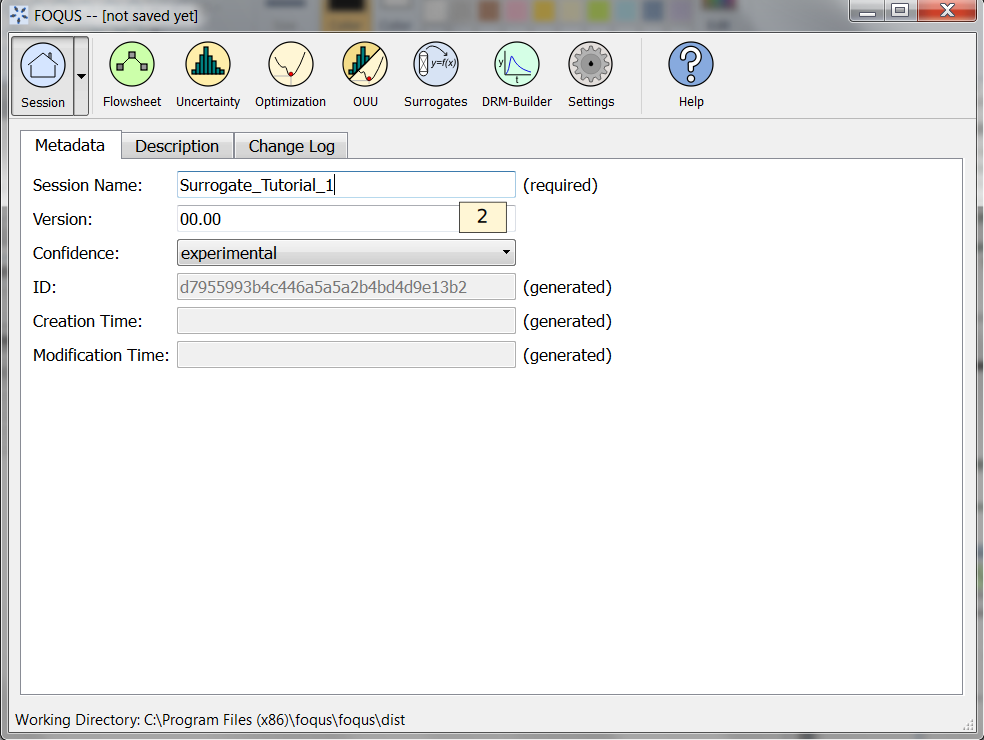
\includegraphics[scale=0.55]{Chapt_surrogates/figs/session1}
		\caption{Session Set Up}
		\label{fig.tut.sur.session}
	\end{center}
\end{figure}

\begin{enumerate}
	\setcounter{enumi}{2}
	\item Navigate to the Flowsheet Editor (Figure \ref{fig.tut.sur.flowsheet}).
	\item Add a Flowsheet Node named ``eq.''
	\item Display the Node Editor by clicking the \textbf{\underline{Node Editor}} toggle button.
\end{enumerate}
\begin{figure}[H]
	\begin{center}
		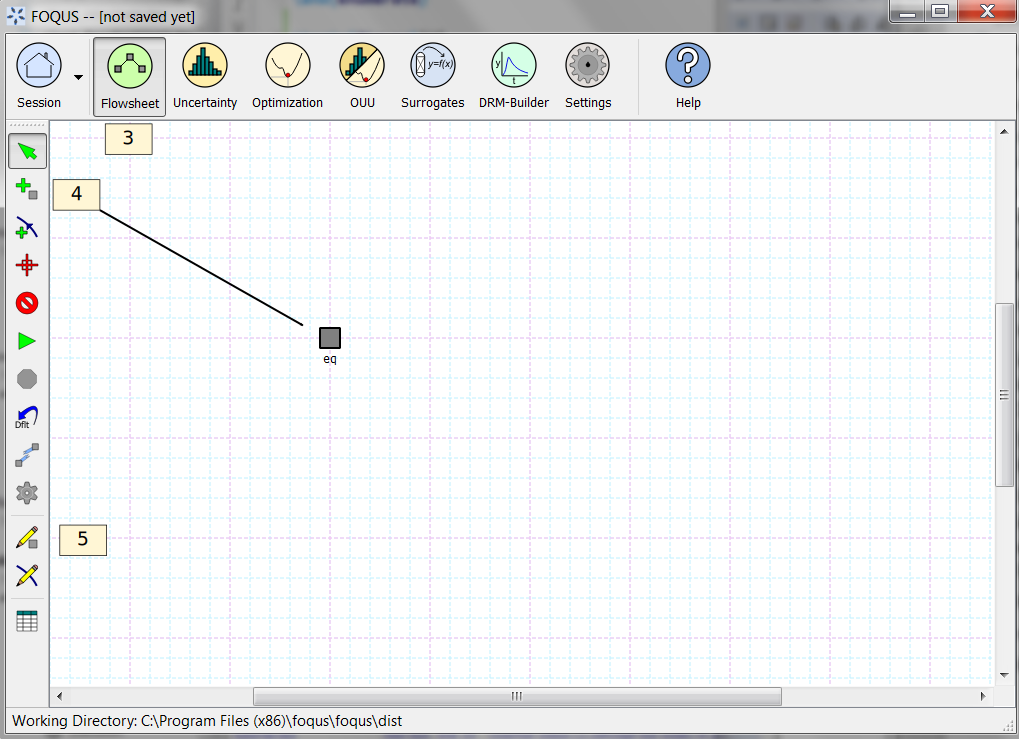
\includegraphics[scale=0.55]{Chapt_surrogates/figs/flowsheet}
		\caption{Flowsheet Setup}
		\label{fig.tut.sur.flowsheet}
	\end{center}
\end{figure}
The \textbf{\underline{Node Editor}} displays (Figure \ref{fig.tut.sur.nodeEdit.Input}).  The first step to setting up the node for this problem is to add input and output variables to the node.
%Does more detail need added to #9 below since the figure shows x1 and x2 in the Input Variables menu. Does the user need to know to click on Output Variables to open the Output Variables screen, then enter z1 and z2 under the Name column?
\begin{enumerate}
	\setcounter{enumi}{5}
	\item If the input variables table is not displayed as shown in Figure \ref{fig.tut.sur.nodeEdit.Input}, click the \textbf{\underline{Variables}} tab and then click the \textbf{\underline{Input Variables}} toolbox section.
	\item Add the variables ``x1'' and ``x2'' by clicking the \textbf{\underline{Add}} icon (+) above the input table.
	\item Edit the \textbf{\underline{Min/Max}} value for both variables to be ``-10.0'' and ``10.0.''
	\item Add two output variables ``z1'' and ``z2.''
\end{enumerate}
\begin{figure}[H]
	\begin{center}
		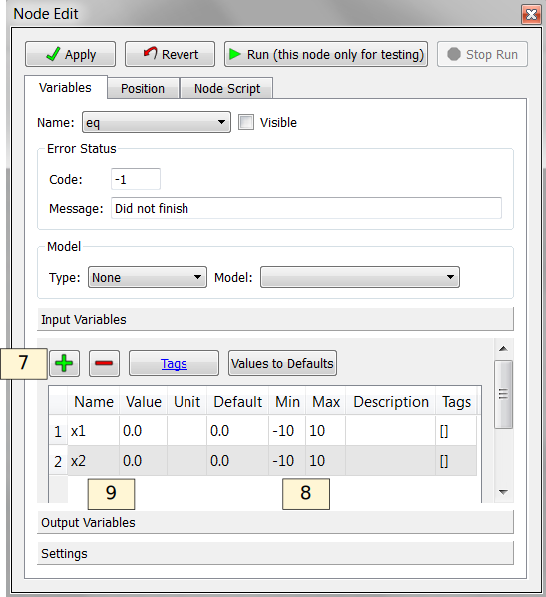
\includegraphics[scale=0.55]{Chapt_surrogates/figs/nodeInput}
		\caption{Node Variables}
		\label{fig.tut.sur.nodeEdit.Input}
	\end{center}
\end{figure}
To keep the execution time short, the node will not be assigned to a simulation model and calculations are performed directly in FOQUS.  
\begin{enumerate}
	\setcounter{enumi}{9}
	\item Click on the \textbf{\underline{Node Script}} tab in the Node Editor to enter the test equation (this step replaces the use of a simulator).
	\item Enter the following equations (Figure \ref{fig.tut.sur.nodeEdit.eq}):
	\begin{verbatim}
		f["z1"] = x["x1"] + x["x2"]
		f["z2"] = x["x1"]**2 + x["x2"]**2
	\end{verbatim}
	The node script calculations are written in Python. The dictionary ``f'' stores output values while the dictionary ``x'' stores input values.

\begin{figure}[H]
	\begin{center}
		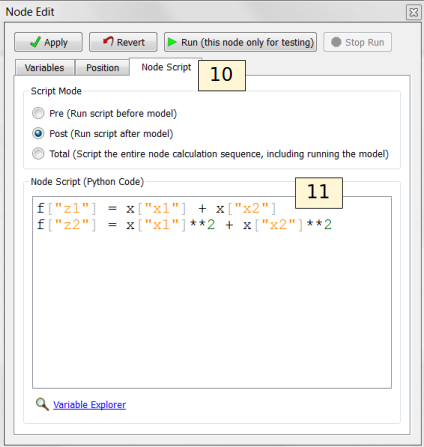
\includegraphics[scale=0.55]{Chapt_surrogates/figs/nodeEq}
		\caption{Node Script}
		\label{fig.tut.sur.nodeEdit.eq}
	\end{center}
\end{figure}

	\item Test the model by running the flowsheet with the value ``2'' for ``x1'' and ``x2.'' After running, the output variables should have the values ``4.0'' for ``z1'' and ``8.0'' for ``z2.''
\end{enumerate}


\subsection{Creating Initial Samples}

There are two ways to start an ALAMO run: (1) generate a set of initial data, (2) use ALAMO's adaptive sampling with no initial data and let ALAMO generates its own samples. Adaptive sampling can be used with initial data to generate more points if needed. In this case, initial data is provided and adaptive sampling is used.

\begin{enumerate}
	\setcounter{enumi}{12}
	\item Select the UQ tool by clicking on the \textbf{\underline{Uncertainty}} button on the Home window (Figure \ref{fig.tut.sur.new.uq.ens}).
	\item Click the \textbf{\underline{Add New}} button.
	\item The \textbf{\underline{Add New Ensemble - Model Selection}} dialog will appear. Click \textbf{\underline{OK}} to set up the sampling scheme.
\end{enumerate}
\begin{figure}[H]
	\begin{center}
		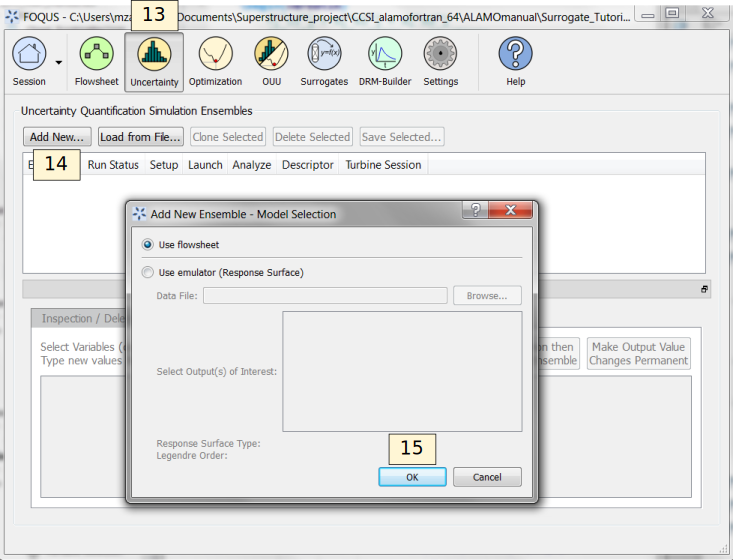
\includegraphics[scale=0.55]{Chapt_surrogates/figs/uqNewEns}
		\caption{Add a New Sample Ensemble}
		\label{fig.tut.sur.new.uq.ens}
	\end{center}
\end{figure}
\begin{enumerate}
	\setcounter{enumi}{15}
	\item The sample ensemble setup dialog displays (Figure \ref{fig.tut.sur.new.uq.sample1}).  Select \textbf{\underline{Choose sampling scheme}}. 
	\item Click the \textbf{\underline{All Variable}} button.
	\item Select the \textbf{\underline{Sampling scheme}} tab.
\end{enumerate}
\begin{figure}[H]
	\begin{center}
		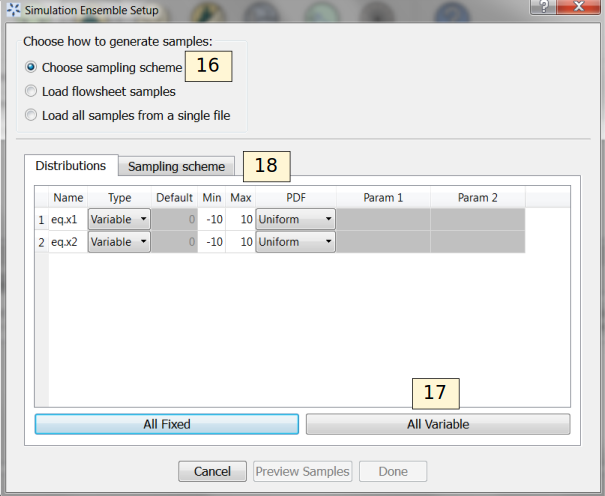
\includegraphics[scale=0.55]{Chapt_surrogates/figs/uqSample1}
		\caption{Sample Distributions}
		\label{fig.tut.sur.new.uq.sample1}
	\end{center}
\end{figure}
\begin{enumerate}
	\setcounter{enumi}{18}
	\item The \textbf{\underline{Sampling schem}e} dialog should display (Figure \ref{fig.tut.sur.new.uq.sample2}). Select ``Latin Hypercube'' from the list.
	\item Set the \textbf{\underline{\# of samples}} to ``10.''
	\item Click \textbf{\underline{Generate Samples}}.
	\item Click \textbf{\underline{Done}}.
\end{enumerate}
\begin{figure}[H]
	\begin{center}
		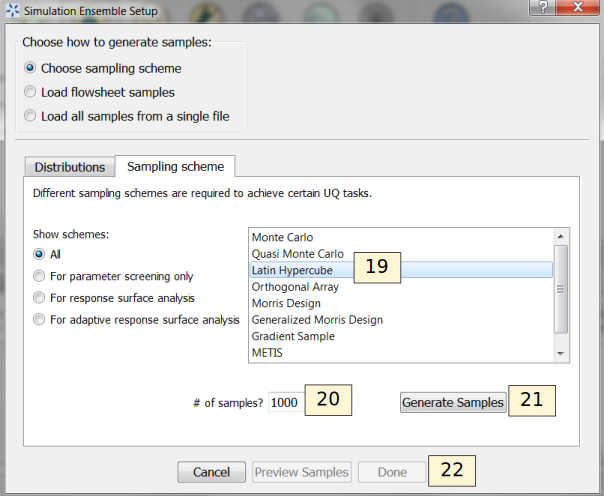
\includegraphics[scale=0.55]{Chapt_surrogates/figs/uqSample2}
		\caption{Sample Methods}
		\label{fig.tut.sur.new.uq.sample2}
	\end{center}
\end{figure}
\begin{enumerate}
\setcounter{enumi}{22}
\item Once the samples have been generated a new sample ensemble displays in the UQ tool window (Figure \ref{fig.tut.sur.new.uq.sample3}).  Click \textbf{\underline{Launch}} to run and generate the samples.
\end{enumerate}
\begin{figure}[H]
	\begin{center}
		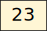
\includegraphics[scale=0.55]{Chapt_surrogates/figs/uqSample3}
		\caption{Run Samples}
		\label{fig.tut.sur.new.uq.sample3}
	\end{center}
\end{figure}

\subsection{Data Selection}

Initial and validation data can be specified by creating filters that specify subsets of flowsheet data. In this tutorial only initial data will be used. A filter must be created to separate the results of the single test run from the UQ samples.

\begin{enumerate}
	\setcounter{enumi}{23}
	\item Click on the \textbf{\underline{Surrogates}} button from the Home window. The surrogate tool displays \ref{fig.tut.sur.data}.
	\item Select ``ALAMO'' from the \textbf{\underline{Tool}} drop-down list.
	\item Click \textbf{\underline{Edit Filters}} in the \textbf{\underline{Flowsheet Results}} section to create a filter.
\end{enumerate} 
\begin{figure}[H]
	\begin{center}
		
\includegraphics[scale=0.55]{Chapt_surrogates/figs/data}
		\caption{Surrogate Data}
		\label{fig.tut.sur.data}
	\end{center}
\end{figure}

\begin{enumerate}
	\setcounter{enumi}{26}
	\item Figure \ref{fig.tut.sur.dataFilter} displays the Data Filter Editor. 
	\item Add the filter for initial data.
	\begin{enumerate}
		\item Click \bu{New Filter}, and enter ``Initial'' as the filter name.
		\item Click \bu{Add Rule}.
		\item In the ``Term 1'' column enter: set (no quotes).
		\item In the ``Term 2'' column enter: ``UQ\_Ensemble'' (with quotes).
		\item In the ``Operator'' column select ``=.''	
	\end{enumerate}
	\item Click \textbf{\underline{Done}}.
\end{enumerate}
\begin{figure}[H]
	\begin{center}
		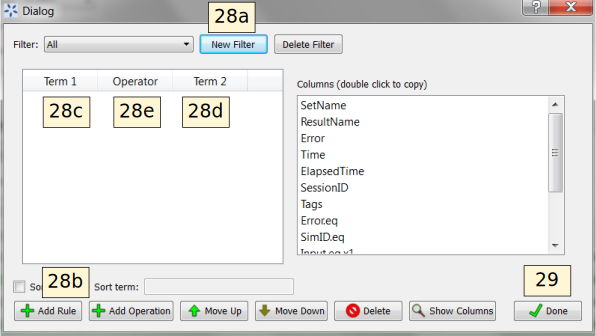
\includegraphics[scale=0.55]{Chapt_surrogates/figs/dataFilter}
		\caption{Data Filter Dialog}
		\label{fig.tut.sur.dataFilter}
	\end{center}
\end{figure}

\subsection{Variable Selection}
In this section, input and output variables need to be selected. Generally, any input variables that vary in the data set should be selected. However, in some cases, variables may be found to have no, or very little, effect on the outputs. Only the output variables of interest need to be selected. Note: Each output is independent from each other and for the model building, selecting one output is the same as selecting more.

\begin{enumerate}
	\setcounter{enumi}{29}
	\item Select the \textbf{\underline{Variable}s} tab (Figure \ref{fig.tut.sur.vaiables}).
	\item Select the checkbox for both input variables.
	\item Select the checkbox for both output variables.
\end{enumerate}
\begin{figure}[H]
	\begin{center}
		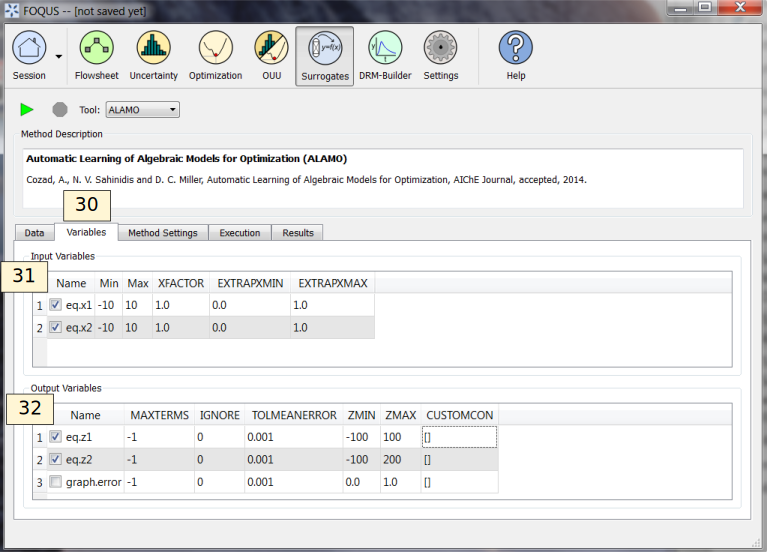
\includegraphics[scale=0.55]{Chapt_surrogates/figs/variables}
		\caption{Variable Selection}
		\label{fig.tut.sur.vaiables}
	\end{center}
\end{figure}

\subsection{Method Settings}
\label{tutorial.alamo.methodsettings}
The most important feature to generate "good" algebraic models is to configure the settings accordingly to the problem to be solved.  Each setting has a good description in FOQUS. The JSON parser is used to read method settings values. Strings must be contained in quotes. Lists have the following format: [element 1, element 2].

\begin{enumerate}
	\setcounter{enumi}{32}
	\item Click on the \textbf{\underline{Method Settings}} tab (see Figure \ref{fig.alamo.method.settigs}).
	\item Set the \textbf{\underline{FOQUS Model (for UQ)}} to ``ALAMO\_tutorial\_UQ.py.'' 
	\item Set the \textbf{\underline{FOQUS Model (for Flowsheet)}} to ``ALAMO\_tutorial\_FS.py''
	\item Set \textbf{\underline{Initial Data Filter}} to ``Initial.''
	\item Set \textbf{\underline{SAMPLER}} to select the adaptive sampling method: ``None'' ``Random'' or ``SNOBFIT.'' Use ``None'' in this tutorial.
	\item Set \textbf{\underline{MONOMIALPOWER}} to select the single variable term powers to [1,2,3].
	\item Set \textbf{\underline{MULTI2POWER}} to select the two variable term powers to [1].
	\item Select functions to be considered as basis functions (\textbf{\underline{EXPFCNS}}, \textbf{\underline{LOGFCNS}}, \textbf{\underline{SINFCNS}}, \textbf{\underline{COSFCNS}}).
	\item Leave the rest of settings as default (see Table \ref{tutorial.alamo.table}).
	\item Save this FOQUS session for use in the ACOSSO and BSS-ANOVA tutorials.
\end{enumerate}
\begin{figure}[H]
	\begin{center}
		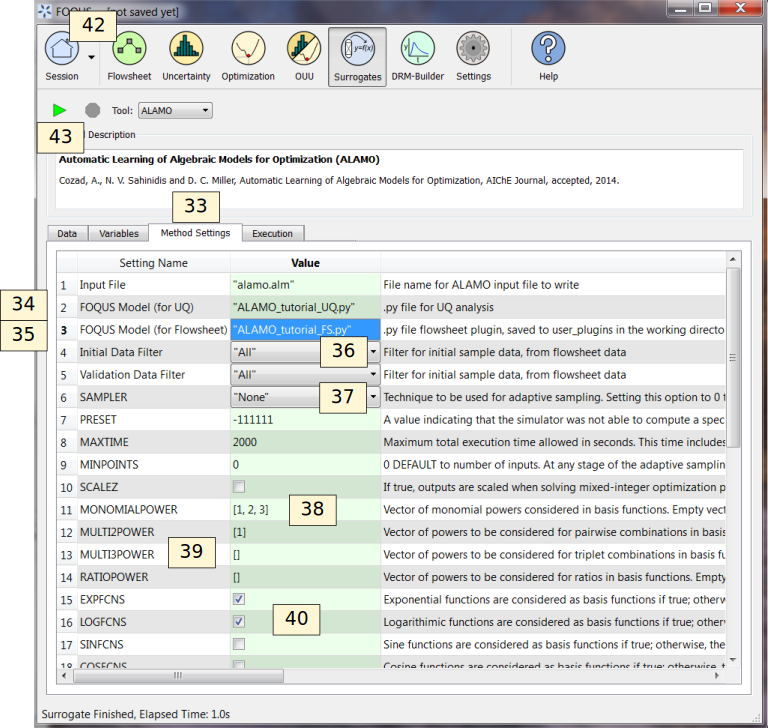
\includegraphics[scale=0.55]{Chapt_surrogates/figs/alamo_settings}
		\caption{ALAMO Method Settings}
		\label{fig.alamo.method.settigs}
	\end{center}
\end{figure}

\subsection{Execution}

\begin{enumerate}
	\setcounter{enumi}{42}
	\item Click the \bu{Run} icon at the top of the window.
	\item The ALAMO \bu{Execution} tab starts displaying execution file path, sub-directories, input files, and output files.
\begin{enumerate}
	\item ALAMO version.
	\item License Information.
	\item Step 0 displays the data set to be used by ALAMO.
	\item Step 1 displays the modeler used by ALAMO to generate the algebraic model.
	\item Once the surrogate model has finished, the equations are displayed in the execution window. It may be necessary to scroll up a little. The result is shown in Figure \ref{fig.alamo.res}.
	\item Finally, the statistics display the quality metrics of the models generated.
\end{enumerate}
\end{enumerate}

\begin{figure}[H]
	\begin{center}
		\includegraphics[scale=0.4]{Chapt_surrogates/figs/alamo_exec}
		\caption{ALAMO Execution}
		\label{fig.alamo.res}
	\end{center}
\end{figure}

\subsection{Results}
	The results are exported as a PSUADE driver file that can be used perform UQ analysis of the models, and a FOQUS Python plugin model that allows it to be used in a FOQUS flowsheet. The equations can also be viewed in the results section.
	
	See tutorial Section \ref{tutorial.surrogate.uq} and \ref{tutorial.surrogate.fs} for information about analyzing the model with the UQ tools or running the model on the flowsheet.
	
	As mentioned in section \ref{tutorial.alamo.methodsettings} the method settings are very important. A brief description and hints are included in Table \ref{tutorial.alamo.table}.

\begin{center}

\begin{longtable}{|p{.30\textwidth}|p{.70\textwidth} |}
\caption{ALAMO Method Settings}
\label{tutorial.alamo.table} \\

		\hline
			\textbf{Method Settings} & \textbf{Description} \\		\hline
			Initial Data Filter & Filter to be applied to the initial data set. Data filters help the user to generate models based on specific data for each variable.  \\	\hline
			Validation Data filter & Data set used to compute model errors at the validation phase. The number of data points in a preexisting validation data set can be specified by the user.\\	\hline
			SAMPLER & Adaptative sampling method to be used. Options: "None", "Random" and "SNOBFIT". Adaptive sampling method to be used by ALAMO when more sampling points are needed by the model. If \bu{Random} is used a simulator must be provided by the user. If \bu{SNOBFIT} is used a simulator must be provided by the user and MATLAB must be installed.\\	\hline
			MAXTIME& Maximum execution time in seconds. This time includes all the steps on the algorithm, if simulations are needed they run in this time.\\	\hline
			MINPOINTS& Convergence is assessed only if the simulator is able to compute the output variables for at least MINPOINTS of the data set. A reduced number of MINPOINTS may reduce the computational time to get a model, but also reduces the accuracy of the model. MINPOINTS must be a positive integer. \\ \hline
			PRESET&Value to be used if the simulator fails. This value must be carefully chosen to be an otherwise not realizable value for the output variables.\\ \hline
			MONOMIALPOWERS &  Vector of monomial powers to be considered as basis functions, use empty vector for none []. Exponential terms allowed in the algebraic model.  i.e., if selecting [1,2] the model considers x1 and x1**2 as basis functions. \\ \hline
			MULTI2POWER & Vector of pairwise combination of powers to be considered as basis functions. Pairwise combination of powers allowed in the algebraic model. i.e., [1,2] allows terms like x1*x2 in the algebraic model.\\ \hline
			MULTI3POWER & Vector of three variables combinations of powers to be considered as basis functions. \\ \hline
			\raggedright{EXPFCNS, LOGFCNS, SINFCNS, COSFCNS functions}& Use or not of exp, log, sin, and cos functions as basis functions in the model. \\ \hline
			RATIOPOWER& Vector of ratio combinations of powers to be considered in the basis functions. Ratio combinations of powers are [empty as default].\\ \hline
			Radial Basis Functions& Radial basis functions centered around the data set provided by the user. These functions are Gaussian and are deactivated if their textual representation requires more than 128 characters (in the case of too many input variables and/or datapoints). \\ \hline
			RBF parameter&Constant penalty used in the Gaussian radial basis functions.  \\ \hline
			Modeler & Fitness metric to be used for model building. Options: BIC (Bayesian Information Criterion), Mallow's Cp, AICc (Corrected Akaike's Information Criterio), HQC (Hannan-Quinn Information Criterion), MSE (Mean Square Error), and Convex Penalty. \\ \hline
			ConvPen& Convex penalty term. Used if Convex Penalty is selected. \\ \hline
			Regularizer & Regularization method is used to reduce the number of potential basis functions before the optimization.\\ \hline 
			Tolrelmetric & Convergence tolerance for the chosen fitness metric is needed to terminate the algorithm. \\ \hline
			ScaleZ&If used, the variables are scaled prior to the optimization problem is solved. The problem is solved using a mathematical programming solver. Usually, scaling the variables may help the optimization procedure.\\ \hline
			GAMS&GAMS is the software used to solve the optimization problems. The executable path is expected or the user must declare GAMS.exe in the environment path.\\ \hline
			GAMS Solver&Solver to be used by GAMS to solve the optimization problems. Mixed integer quadratic programming solver is expected like BARON (other solvers can be used).\\ \hline
			MIPOPTCR & Relative convergence tolerance for the optimization problems solved in GAMS. The optimization problem is solved when the optcr is reached. 5 to 1 \% is expected (0.005 to 0.001).\\ \hline
			MIPOPTCA & Absolute convergence tolerance for mixed-integer optimization problems. This must be a nonnegative scalar. \\ \hline
			Linear error & If true, a linear objective function is used when solving the mixed integer optimization problems; otherwise, a quadratic objective function is used. \\ \hline
			\raggedright{Constraint Regression (CONREG)} & Specify whether constraint regression is used or not, if true bounds on output variables are enforced. \\ \hline
			CRNCUSTOM & If true, Custom constraints are entered in the Variable tab.\\ \hline
			CRNINITIAL& Number of random bounding points at which constraints are sampled initially (must be a nonnegative integer). \\ \hline
			CRNMAXITER & Maximum allowed constrained regressions iterations. Constraints are enforced on additional points during each iteration (must be positive integer). \\ \hline
			CRNVIOL & Number of bounding points added per round per bound in each iteration (must be positive integer). \\ \hline
			CRNTRIALS&Number of random trial bounding points per round of constrained regression (must be a positive integer). \\ \hline
			CUSTOMBAS&A list of user-supplied custom basis functions can be provided by the user. The parser is not case sensitive and allows for any Fortran functional expression in terms of the XLABELS (symbol \^{} may be used to denote power). \\ \hline
			
%		\end{tabularx}
%	\end{center}

\end{longtable}	
\end{center}	

\section{Tutorial -- ACOSSO}
\label{(sec.surrogate.acosso)}

This tutorial covers the ACOSSO surrogate modeling method. The Adaptive
COmponent Selection and Shrinkage Operator (ACOSSO) surface approximation
was developed under the Smoothing Spline Analysis of Variance (SS-ANOVA)
modeling framework \citep{Storlie_2011}. As it is a smoothing type method,
ACOSSO works best when the underlying function is somewhat smooth. For
functions which are known to have sharp changes or peaks, etc., other
methods may be more appropriate. Since it implicitly performs variable
selection, ACOSSO can also work well when there are a large number of input
variables. 
The ACOSSO procedure also allows for
categorical inputs \citep{Storlie_2013}.
 
This tutorial uses the same flowsheet and sample setup as the ALAMO
tutorial in Section \ref{sec.surrogate.alamo}. The statistics software
``R'' is also required to use ACOSSO and BSS-ANOVA. Before starting this
tutorial, you will need to install R version 3.1 or later (see \href{http://cran.r-project.org/}{\textcolor{blue}{https://cran.r-project.org/}}). 

Once R is installed, you will need to install the ``quadprog''
package. ACOSSO requires this package for solving quadratic
programming problems. You will only need to perform this step once. 

\begin{enumerate}
\item{Start R. In Windows, this must be done with administrative
  privileges.  Either run this from an administrator account, or
  right-click ``R x64 3.1.2'' and click ``Run with administrator'' and type
  in administrator credentials.}
\item{Inside the R console, type:
   \begin{itemize} 
   \item \tt install.packages('quadprog')
   \item \tt library(quadprog)
   \item \tt q()
  \end{itemize}
The first line installs the package. If prompted for a CRAN mirror, select
the one closest to you geographically. The second line loads the
package. The last line quits R. If prompted to save workspace image, choose
`y'.}
\end{enumerate}

Once you have done these steps, ACOSSO is ready to be invoked inside FOQUS.

\begin{enumerate}
	\item{Set the path to the RScript executable.}
		\begin{enumerate}
			\item Click the \bu{Settings} button in the Home window.
			\item Change the RScript path if necessary. The \bu{Browse} button
           opens a file browser that can be used to set the path.
		\end{enumerate}
	\item Complete the ALAMO tutorial in Section \ref{sec.surrogate.alamo} through Step 32, or load the FOQUS session saved after completing the ALAMO tutorial.
	\item Click the \bu{Surrogates} button in the Home window (Figure \ref{fig.acosso.settings}).
	\item Select ``ACOSSO'' in the \bu{Tool} drop-down list.
	\item Select the \bu{Method Settings} tab.
	\item Set ``Data Filter'' to ``Initial.''
	\item Set ``Use Flowsheet Data'' to ``Yes.''
	\item Set ``FOQUS Model (for UQ)'' to ``ACOSSO\_Tutorial\_UQ.py.''
	\item Set ``FOQUS Model (for Flowsheet)'' to ``ACOSSO\_Tutorial\_FS.py.''
	\item Click the \bu{Run} icon (Figure \ref{fig.acosso.settings}).
\end{enumerate}

\begin{figure}[H]
	\begin{center}
		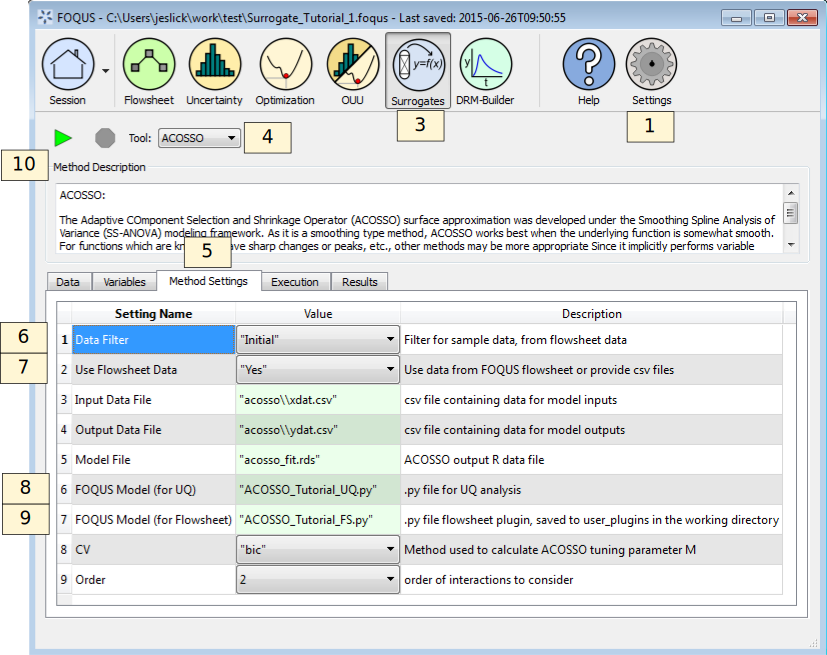
\includegraphics[scale=0.55]{Chapt_surrogates/figs/acosso_settings}
		\caption{ACOSSO Session Set Up}
		\label{fig.acosso.settings}
	\end{center}
\end{figure}

\begin{enumerate}
	\setcounter{enumi}{10}
	\item The execution window will automatically display. While ACOSSO is
     running, the execution window may show warnings, but this is normal.
	\item When the run completes, a UQ driver file is created, allowing the
     ACOSSO surrogate to be used as a user-defined response surface in UQ
     analyses. (See Section \ref{tutorial.surrogate.uq}.)
	\item ACOSSO also produces a flowsheet plugin; however.
\end{enumerate}



\section{Tutorial -- BSS-ANOVA}
\label{(sec.surrogate.bssanova)}

This tutorial covers the BSS-ANOVA surrogate modeling method.  The Bayesian
Smoothing Spline ANOVA (BSS-ANOVA) is essentially a Bayesian version of
ACOSSO \citep{Reich_2009}.  It is Gaussian Process (GP) model with a
non-conventional covariance function that borrows its form from SS-ANOVA.
It tackles the high dimensionality (of inputs) on two fronts: (1) variable
selection to eliminate uninformative variables from the model and (2)
restricting the level of interactions involved among the variables in the
model. This is done through a fully Bayesian approach which can also allow
for categorical input variables with relative ease. Since it is closely
related to ACOSSO, it generally works well in similar settings as
ACOSSO. The BSS-ANOVA procedure also allows for categorical inputs
\citep{Storlie_2013}. In this current implementation, BSS-ANOVA is more
computationally intensive than ACOSSO, so ACOSSO is preferred for faster
surrogate generation. 

This tutorial uses the same flowsheet and sample setup as the ALAMO
tutorial in Section \ref{sec.surrogate.alamo}. The statistics software
``R'' is also required to use ACOSSO and BSS-ANOVA. Before starting this
tutorial, you will need to install R version 3.1 or later (see \href{https://cran.r-project.org/}{\textcolor{blue}{http://cran.r-project.org/}}).

\begin{enumerate}
	\item{Set the path to the RScript executable.}
		\begin{enumerate}
			\item Click the \bu{Settings} button from the Home window.
			\item Change the RScript path if necessary.  The \bu{Browse} button opens a file browser that can be used to set the path.
		\end{enumerate}
	\item Complete the ALAMO tutorial in Section \ref{sec.surrogate.alamo} through Step 32, or load the FOQUS session saved after completing the ALAMO tutorial.
	\item Click the \bu{Surrogates} button from the Home window (Figure \ref{fig.bssanova.settings}).
	\item Select ``BSS-ANOVA'' in the \bu{Tool} drop-down list.
	\item Select the \bu{Method Settings} tab.
	\item Set ``Data Filter'' to ``Initial.''
	\item Set ``Use Flowsheet Data'' to ``Yes.''
	\item Set ``FOQUS Model (for UQ)'' to ``bssanova\_tutorial\_uq.py.''
	\item Set ``FOQUS Model (for Flowsheet)'' to ``bssanova\_tutorial\_fs.py.''
	\item Click the \bu{Run} icon (Figure \ref{fig.bssanova.settings}).
\end{enumerate}

\begin{figure}[H]
	\begin{center}
		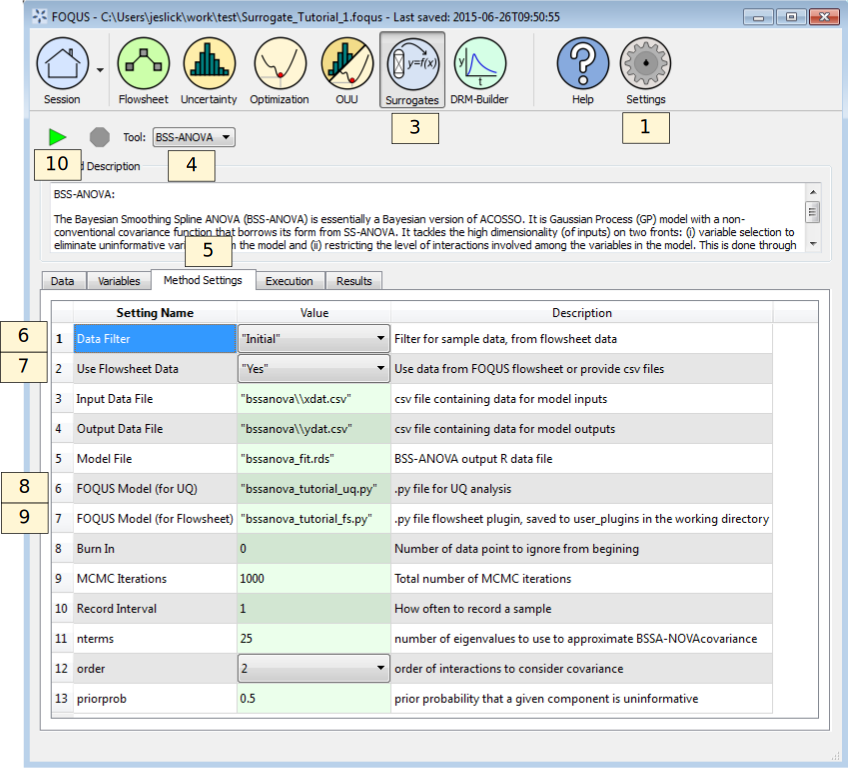
\includegraphics[scale=0.55]{Chapt_surrogates/figs/bssanova_settings}
		\caption{BSS-ANOVA Session Set Up}
		\label{fig.bssanova.settings}
	\end{center}
\end{figure}

\begin{enumerate}
   \setcounter{enumi}{10}
   \item The execution window will automatically display. While BSS-ANOVA is
     running, the execution window may show warnings, but this is normal.
   \item When the run completes, a UQ driver file is created, allowing the
     BSS-ANOVA surrogate to be used as a user-defined response surface in UQ
     analyses. (See Section \ref{tutorial.surrogate.uq}.)
   \item BSS-ANOVA also produces a flowsheet plugin.
\end{enumerate}


\section{Tutorial -- iREVEAL} 
The iREVEAL documentation is currently separate, but will be merged in the next release. The iREVEAL user's manual is included in the FOQUS installation.  There is a link to the manual in the Windows start menu under CCSI Tools\bs FOQUS.

\section{Tutorial -- Surrogates with UQ Tools}
\label{tutorial.surrogate.uq}

For the purpose of this tutorial, we will use ACOSSO to demonstrate the use
of a surrogate within the UQ module. The steps are the same regardless of
the surrogate tool chosen.

To perform the UQ analysis, Python is required for use the ``User Regression'' response surface that will be used.  Before starting this tutorial, you will need to install Python 2.7.x (not Python 3). (See \href{https://www.python.org/downloads/}{\textcolor{blue}{https://www.python.org/downloads/}}). In addition, if *.py files have been re-associated with other executables (e.g. editors), please change the association back to python.exe. 


\begin{enumerate}
\item{Load a fresh session by clicking the \bu{Session} button from the Home window. Select \textbf{\underline{Open Session}} and then navigate to the ``examples/UQ''
  directory. Select ``Rosenbrock\_no\_vectors.foqus.'' This will load a
  session with a simple flowsheet containing a single node.}
\item{Click \bu{Settings} and ensure that (1) FOQUS Flowsheet Run Method is
  set to ``Local'', and that (2) proper paths are set for PSUADE and RScript.} 
\item{Train an ACOSSO surrogate of this node by clicking the
  \bu{Surrogates} button from the Home window.
\begin{enumerate}
\item{Click \bu{Add Samples} and select ``Use Flowsheet''. This will
  display the \bu{Simulation Ensemble Setup} dialog.}
\item{Within this dialog, ensure all variables are set to ``Variable''
  type in the \bu{Distributions} tab. In the \bu{Sampling scheme} tab,
  select ``Monte Carlo'' as your sampling scheme, set the number of
  samples to 100, and then click \bu{Generate Samples} to generate the
  set of input values. Click \bu{Done} to return to the Surrogates screen.}
\item{Once sample generation completes, click the \bu{Uncertainty} button from the Home window.}
\item{Click the \bu{Launch}	button to generate the samples.}
\item{Click the \bu{Surrogates} button from the Home window. The \bu{Data} tab of the Surrogates
  screen should now displays a \bu{Flowsheet Results} table that is populated with
  the values of the new input samples.}
\item{From the \bu{Variables} tab, select all of the checkboxes. (There should
  be six checkboxes for input variables and one checkbox for output variable.) 
  Here, you are defining the inputs and outputs for your surrogate function.}
\item{From the \bu{Method Settings} tab, note the name of the file next to
  ``FOQUS Model (for UQ)''. This will be the name of the UQ driver file
  that contains the Python code that implements the surrogate function.}
\item{On top of this screen, select ``ACOSSO'' as your surrogate tool from the \textbf{\underline{Tool}} drop-down list and then click on the green arrow to start training the surrogate.}
\item{Once complete, a popup window will display, reminding you of the
  location of the drive file. Note the location as you will need this
  information later inside the UQ module.} 
\end{enumerate}
}
\item{Perform a response-surface-based uncertainty analysis by clicking the 
  \bu{Uncertainty} button from the Home window.
\begin{enumerate}
\item{In the \bu{Uncertainty Quantification Simulation Ensembles} table. A row corresponding to the ensemble that was just
  generated for surrogate training should be displayed. This same ensemble can be used or
  a new one can be created to be used as the test data set for analysis. 
  In the row corresponding to the ensemble
  to be analyzed, click the \bu{Analyze} button to proceed. This
  action will bring up an analysis dialog.} 
\item{Within this analysis dialog, navigate to ``Analysis'' section. For
  Step 1, select ``Response Surface''. For Step 3, select ``User
  Regression'' in the first drop-down list. Lastly, for ``User Regression File'',
  browse to the same location as the UQ driver file that was
  generated within the Surrogates module. (This is the same location that
  was previously noted from the popup message.) 
  At this point, your surrogate function is now set up as a user-defined
  response surface and all response-surface-based UQ analyses are accessible.}
\item{Click \bu{Validate} (Step 4) to perform response surface validation. Once
  complete, a figure with cross-validation results will be displayed: 
  a histogram of errors to the left and a plot of predicted values versus
  actual values to the right. For more information, refer to the UQ
  Tutorial in Section \ref{tutorial.uq.rs}.}
\item{Once a ``Response Surface'' has been validated, other UQ analysis options
  are available. Choose ``Uncertainty Analysis'' in Step 5 and click
  \bu{Analyze} to perform uncertainty analysis using your ACOSSO surrogate.}
\end{enumerate}
}
\end{enumerate}

During validation, if the error, ``RSAnalyzer: RSTest\_hs.m does
not exist.'' displays, this is likely caused by incompatibility with the surrogate
and the test data. An example scenario might be your test data has six
inputs, but your surrogate assumes five inputs. This is easily fixed by
returning to the Surrogates screen, clicking on the \bu{Variables}
tab, and making sure the appropriate selections are made (i.e., check off six
inputs instead of just five).

\section{Tutorial -- Surrogates with the Flowsheet}\label{tutorial.surrogate.fs}

This section provides a brief tutorial for using the flowsheet plugin models generated by surrogate modeling methods. In the next FOQUS release all surrogate modeling methods will produce a model that can be run in a FOQUS flowsheet. \textbf{Currently iREVEAL does not produce a flowsheet model.}

\textbf{Before doing this tutorial complete the ALAMO tutorial in Section \ref{sec.surrogate.alamo}.}

\begin{enumerate}
	\item Open FOQUS.  If FOQUS has not been closed since completing the ALAMO tutorial, close it and reopen it. There is a known issue where existing flowsheet model plugins may not update until FOQUS is restarted.
	\item Enter ``FS\_Plugin\_Tutorial'' as the Session Name.
	\item Click the \bu{Flowsheet} button from the Home window.
	\item Click the \bu{Add Node} icon in the left toolbar (see Figure \ref{fig.pg.tut1}).
	\item Click a location for the node in the Flowsheet area.
	\item Enter ``model'' for the node name (without quotes).
	\item Click the \bu{Node Editor} icon in the left toolbar (see Figure \ref{fig.pg.tut1}).
	\item In the \textbf{\underline{Node Editor}}, select ``Plugin'' from the Model \textbf{\underline{Type}} drop-down list. 
	\item Select ``ALAMO\_Tutorial\_FS'' from the \textbf{\underline{Model}} drop-down list. 
	\item Set the \textbf{\underline{Value}} of the \textbf{\underline{Input Variables}} ``eq.x1'' to 2.
	\item Set the \textbf{\underline{Value}} of the \textbf{\underline{Input Variables}} ``eq.x2'' to 3.
	\item Click the \bu{Run} icon in the left toolbar (see Figure \ref{fig.pg.tut1}).
	\item Wait for the Flowsheet evaluation to complete. It should finish successfully.
	\item Check the value of the \textbf{\underline{Output Variables}}; the approximate values should be z1 = 5 and z2 = 13.
\end{enumerate}

\begin{figure}[H]
	\begin{center}
		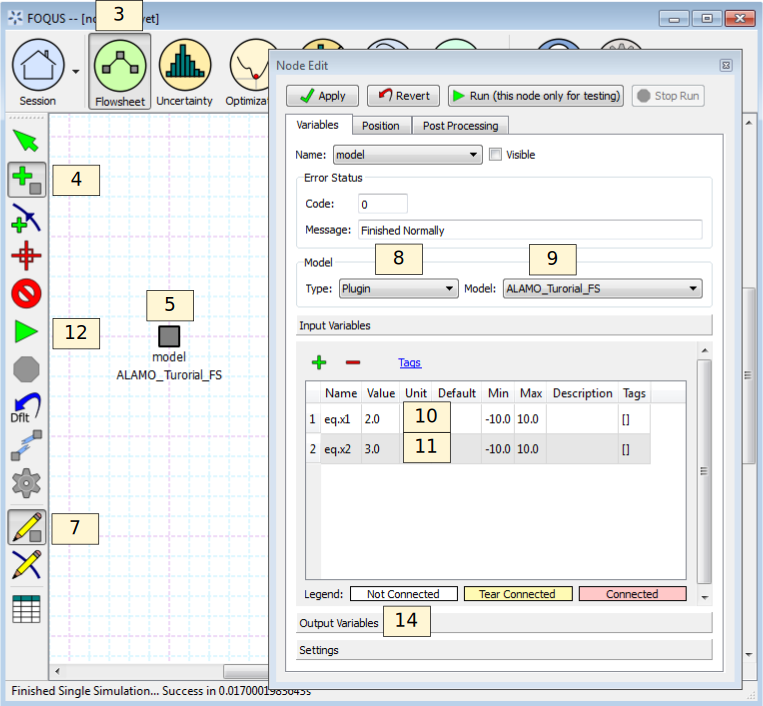
\includegraphics[scale=0.55]{Chapt_surrogates/figs/fs_plugin}
		\caption{Plugin Flowsheet}
		\label{fig.pg.tut1}
	\end{center}
\end{figure}




	

\chapter{Surrogate Models}\label{chpt.surrogates}

\section{D-RM (Dynamic Reduced Models) Builder}\label{sec.overview.drm}

The Dynamic Reduced Model (D-RM) Builder is a software tool used to generate data-driven dynamic reduced models from high-fidelity dynamic models consisting of differential and algebraic equations (DAEs).  DAE-based models are usually computationally intensive to solve, especially when stiff DAEs are involved.  For instance, the sorbent-based bubbling fluidized bed CO$_2$ adsorber-reactor model contains over 20,000 DAEs and very small time steps ($<$0.001 second) have to be used to solve the stiff equations in the rigorous model.  The D-RMs generated by the D-RM Builder enable much faster computation of the system responses (up to several orders of magnitude faster), which enable the development of an advanced process control framework and the integration of the dynamic models within a large-scale dynamic simulation.

\subsection{Motivating Example}

The solid-sorbent-based bubbling fluidized bed CO$_2$ adsorber-reactor for the post-combustion carbon capture is a good example to which the D-RM Builder tool can be applied.  The dynamics of the adsorber-reactor was modeled by a CCSI team using Aspen Custom Modeler (ACM).  The high-fidelity dynamic model of the twin-bed adsorber-reactor contains over 20,000 equations.  The feed streams include CO$_2$-containing flue gas, solid sorbent, and multiple cooling water streams.  Since some equations are very stiff, a minimum integration time step of 0.001 second has to be used.  As a result, the computer CPU time required to calculate the response of the system over a period of operating time is much longer than the real operating time, especially when there is a change in model inputs (step or ramp change).  The data-driven D-RM can be generated by fitting the system outputs in response to the changes of system inputs through certain plant identification models.  The response of the system to the input changes can be simulated by the ACM model.  The D-RM Builder is provided for a user to configure the input and output variables of interest, prepare a sequence of step changes of input variables, launch ACM simulations, generate a D-RM, and export the D-RM in a form of a MATLAB function file (.m file), which can be called by MATLAB to calculate the system response given the model inputs with a CPU execution time a few orders of magnitude shorter than that required by the ACM model.  The speedup in CPU time enables the implementation of advanced process control (APC) systems.

\subsection{Features List}

The D-RM Builder is an application embedded in the graphic user interface (GUI) of FOQUS.  Data-driven D-RMs can be generated by the D-RM Builder based on a set of high-fidelity model outputs in response to a sequence of input changes within a range of operating conditions.  The D-RM Builder can read the input and output variables pre-configured through SinterConfigGUI application, which is also a part of the FOQUS package.  Through the D-RM Builder GUI, a user can select a set of the pre-configured input variables, specify their lower and upper limits, and prepare a sequence of step changes or ramp changes based on the Latin Hypercube Sampling (LHS) method with desired durations of the step changes to excite the system in a range of frequencies.  The simulations of high-fidelity models, currently implemented for ACM only, can be launched directly in the D-RM Builder through ConsoleSinter, which is also a part of the FOQUS package.  The simulation results can be used to generate the D-RMs.  A separate set of step-change sequence can also be generated and its response be simulated by the ACM model and predicted by the D-RM for validation purpose.  The generated D-RMs and the user inputs for case setup and configuration can be saved in a text file in JSON format with extension ``drmb''.  Once a case file is saved, the user can copy the file to a different directory or to a different computer where the D-RM Builder is installed and open the file later to continue the D-RM building process or visualize the properties of the generated D-RMs.  A D-RM Builder project could also be a subproject of a FOQUS project and saved as a part of FOQUS session.  When a saved FOQUS session file is opened, the D-RM Builder subproject is also opened.

Two types of D-RMs are supported in the current version including the Decoupled A-B Net (DABNet) model \cite{Sentoni_1998}, and the Nonlinear Auto-regressive Moving Average (NARMA) model \cite{Narendra_1997}.  Different building options are provided for the user to choose from including input delays, two-pole Laugerre formulation of DABNet model, and optimization of model parameters.  Both D-RM model types require the training of artificial neural networks (ANNs).  Two ANN training methods, back propagation (BP) and interior point optimization (IPOPT), are provided.  The generated D-RM can be validated by performing another set of high-fidelity model simulations with a different input change sequence and comparing the response to that predicted by the generated D-RMs.  The response calculated by the high-fidelity model and that by the D-RM can be displayed through the D-RM Builder$\text{'}$s GUI.  The accuracy of the generated D-RM can be visualized by comparing the D-RM predictions to the corresponding ACM predictions, including the relative errors and the coefficient of determination R$^2$.  For the state-space based DABNet model, Uncertainty Quantification (UQ) analysis can be performed on the validation data using Unscented Kalman Filter (UKF), providing the covariance matrices of state-space and output variables.  The messages of the model building process including command sequence are displayed in the main text window of the D-RM Builder, which can be saved to a log file for future reference.  The internal parameters of the generated D-RM can be exported to a MATLAB script file, which can be run in MATLAB to initialize a D-RM object instantiated from a MATLAB class.  The results of the high-fidelity model simulations and D-RM predictions for both the training and the validation input sequences can also be exported to text files in comma-separated value (CSV) format, which can be opened by Microsoft® Excel®.

Along with the D-RM Builder application, several MATLAB files are also provided as part of the software tool.  These files define the MATLAB classes that can be used to create the D-RM objects in the MATLAB workspace given the D-RM files exported from the D-RM Builder.  The functions in the D-RM objects can be called to perform dynamic simulations.

\section{Tutorial -- ALAMO}
\label{sec.surrogate.alamo}
This tutorial focuses on the use of the ALAMO tool for building algebraic surrogate models. ALAMO builds simplified algebraic models, which are particularly well suited for rigorous equation oriented optimization. To keep the execution of this tutorial fast, a toy problem is used. In this case study the flowsheet calculations and sample generation are done within FOQUS, alternatively, the user can provide a simulation model such as: Excel, Aspen plus, Aspen custom modeler, etc. 

Note: Before starting this tutorial the ALAMO product must be downloaded from the products page on the CCSI website. The path for the ALAMO executable file must be set in FOQUS settings (see Section \ref{section.settings}).

\subsection{Flowsheet Setup}

\begin{enumerate}
	\item Open FOQUS.
	\item Name the session ``Surrogate\_Tutorial\_1'' (Figure \ref{fig.tut.sur.session}).
\end{enumerate}

\begin{figure}[H]
	\begin{center}
		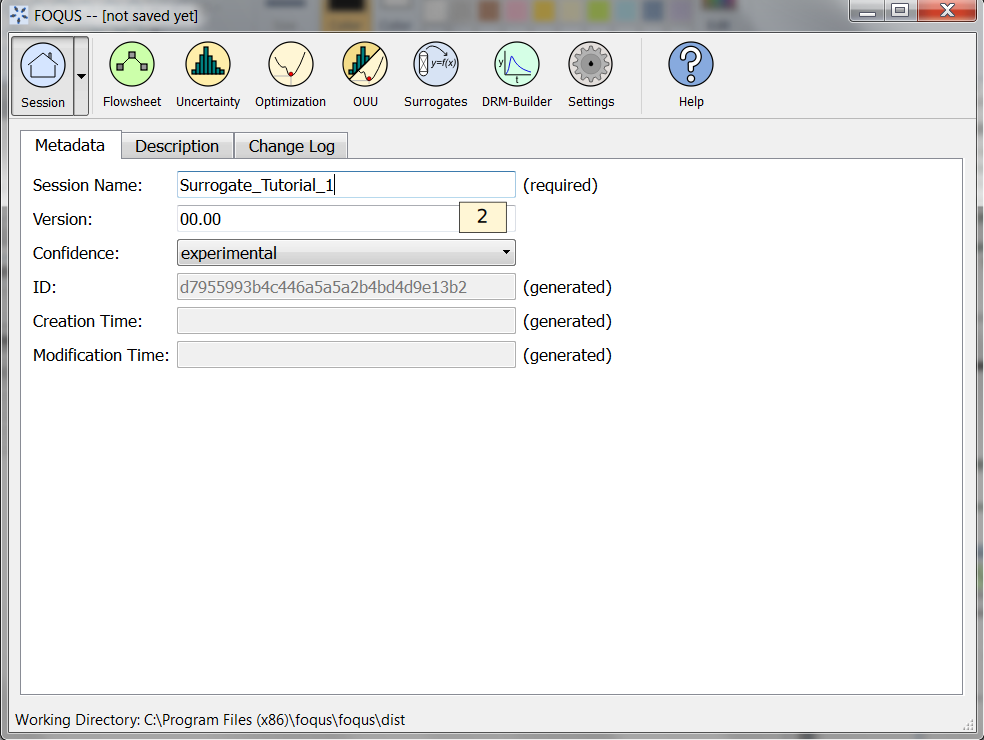
\includegraphics[scale=0.55]{Chapt_surrogates/figs/session1}
		\caption{Session Set Up}
		\label{fig.tut.sur.session}
	\end{center}
\end{figure}

\begin{enumerate}
	\setcounter{enumi}{2}
	\item Navigate to the Flowsheet Editor (Figure \ref{fig.tut.sur.flowsheet}).
	\item Add a Flowsheet Node named ``eq.''
	\item Display the Node Editor by clicking the \textbf{\underline{Node Editor}} toggle button.
\end{enumerate}
\begin{figure}[H]
	\begin{center}
		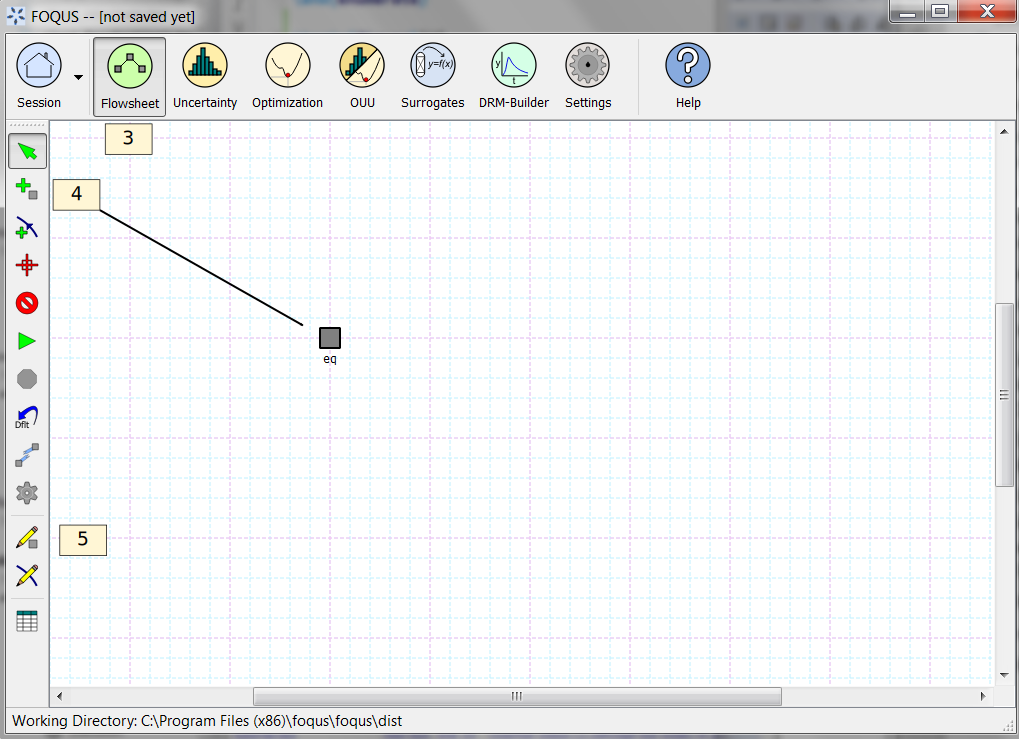
\includegraphics[scale=0.55]{Chapt_surrogates/figs/flowsheet}
		\caption{Flowsheet Setup}
		\label{fig.tut.sur.flowsheet}
	\end{center}
\end{figure}
The \textbf{\underline{Node Editor}} displays (Figure \ref{fig.tut.sur.nodeEdit.Input}).  The first step to setting up the node for this problem is to add input and output variables to the node.
%Does more detail need added to #9 below since the figure shows x1 and x2 in the Input Variables menu. Does the user need to know to click on Output Variables to open the Output Variables screen, then enter z1 and z2 under the Name column?
\begin{enumerate}
	\setcounter{enumi}{5}
	\item If the input variables table is not displayed as shown in Figure \ref{fig.tut.sur.nodeEdit.Input}, click the \textbf{\underline{Variables}} tab and then click the \textbf{\underline{Input Variables}} toolbox section.
	\item Add the variables ``x1'' and ``x2'' by clicking the \textbf{\underline{Add}} icon (+) above the input table.
	\item Edit the \textbf{\underline{Min/Max}} value for both variables to be ``-10.0'' and ``10.0.''
	\item Add two output variables ``z1'' and ``z2.''
\end{enumerate}
\begin{figure}[H]
	\begin{center}
		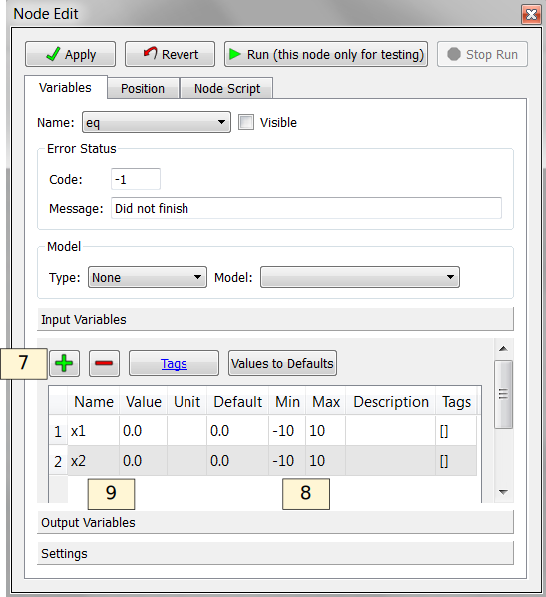
\includegraphics[scale=0.55]{Chapt_surrogates/figs/nodeInput}
		\caption{Node Variables}
		\label{fig.tut.sur.nodeEdit.Input}
	\end{center}
\end{figure}
To keep the execution time short, the node will not be assigned to a simulation model and calculations are performed directly in FOQUS.  
\begin{enumerate}
	\setcounter{enumi}{9}
	\item Click on the \textbf{\underline{Node Script}} tab in the Node Editor to enter the test equation (this step replaces the use of a simulator).
	\item Enter the following equations (Figure \ref{fig.tut.sur.nodeEdit.eq}):
	\begin{verbatim}
		f["z1"] = x["x1"] + x["x2"]
		f["z2"] = x["x1"]**2 + x["x2"]**2
	\end{verbatim}
	The node script calculations are written in Python. The dictionary ``f'' stores output values while the dictionary ``x'' stores input values.

\begin{figure}[H]
	\begin{center}
		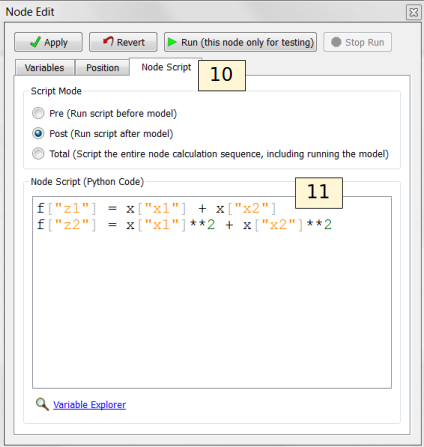
\includegraphics[scale=0.55]{Chapt_surrogates/figs/nodeEq}
		\caption{Node Script}
		\label{fig.tut.sur.nodeEdit.eq}
	\end{center}
\end{figure}

	\item Test the model by running the flowsheet with the value ``2'' for ``x1'' and ``x2.'' After running, the output variables should have the values ``4.0'' for ``z1'' and ``8.0'' for ``z2.''
\end{enumerate}


\subsection{Creating Initial Samples}

There are two ways to start an ALAMO run: (1) generate a set of initial data, (2) use ALAMO's adaptive sampling with no initial data and let ALAMO generates its own samples. Adaptive sampling can be used with initial data to generate more points if needed. In this case, initial data is provided and adaptive sampling is used.

\begin{enumerate}
	\setcounter{enumi}{12}
	\item Select the UQ tool by clicking on the \textbf{\underline{Uncertainty}} button on the Home window (Figure \ref{fig.tut.sur.new.uq.ens}).
	\item Click the \textbf{\underline{Add New}} button.
	\item The \textbf{\underline{Add New Ensemble - Model Selection}} dialog will appear. Click \textbf{\underline{OK}} to set up the sampling scheme.
\end{enumerate}
\begin{figure}[H]
	\begin{center}
		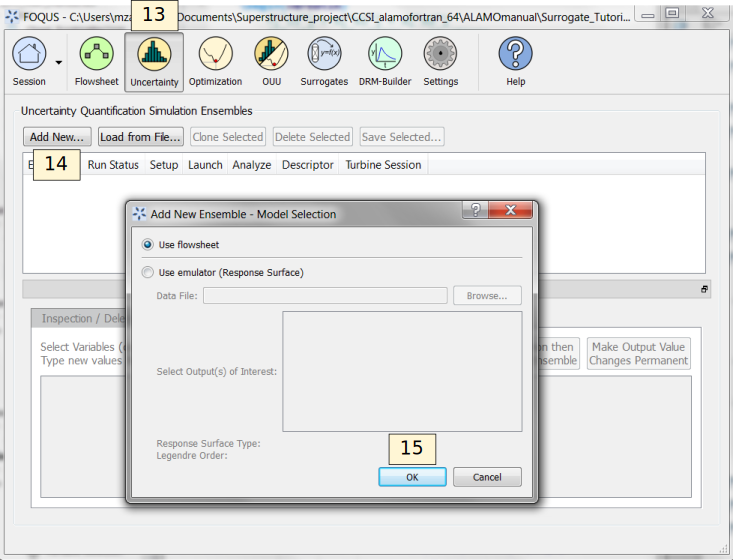
\includegraphics[scale=0.55]{Chapt_surrogates/figs/uqNewEns}
		\caption{Add a New Sample Ensemble}
		\label{fig.tut.sur.new.uq.ens}
	\end{center}
\end{figure}
\begin{enumerate}
	\setcounter{enumi}{15}
	\item The sample ensemble setup dialog displays (Figure \ref{fig.tut.sur.new.uq.sample1}).  Select \textbf{\underline{Choose sampling scheme}}. 
	\item Click the \textbf{\underline{All Variable}} button.
	\item Select the \textbf{\underline{Sampling scheme}} tab.
\end{enumerate}
\begin{figure}[H]
	\begin{center}
		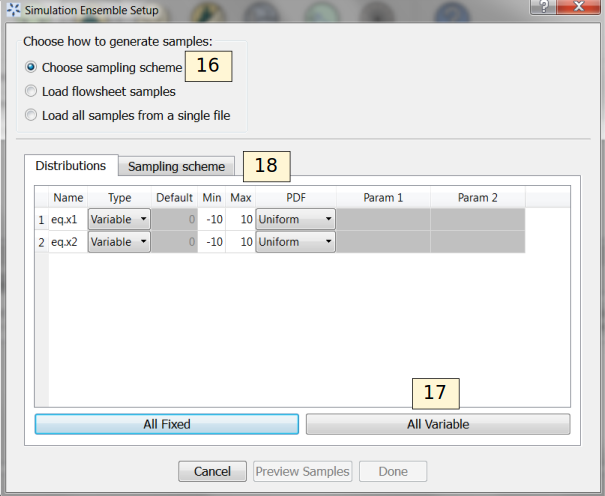
\includegraphics[scale=0.55]{Chapt_surrogates/figs/uqSample1}
		\caption{Sample Distributions}
		\label{fig.tut.sur.new.uq.sample1}
	\end{center}
\end{figure}
\begin{enumerate}
	\setcounter{enumi}{18}
	\item The \textbf{\underline{Sampling schem}e} dialog should display (Figure \ref{fig.tut.sur.new.uq.sample2}). Select ``Latin Hypercube'' from the list.
	\item Set the \textbf{\underline{\# of samples}} to ``10.''
	\item Click \textbf{\underline{Generate Samples}}.
	\item Click \textbf{\underline{Done}}.
\end{enumerate}
\begin{figure}[H]
	\begin{center}
		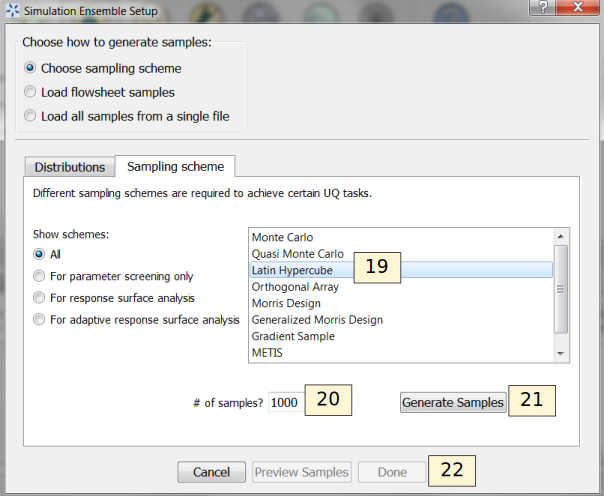
\includegraphics[scale=0.55]{Chapt_surrogates/figs/uqSample2}
		\caption{Sample Methods}
		\label{fig.tut.sur.new.uq.sample2}
	\end{center}
\end{figure}
\begin{enumerate}
\setcounter{enumi}{22}
\item Once the samples have been generated a new sample ensemble displays in the UQ tool window (Figure \ref{fig.tut.sur.new.uq.sample3}).  Click \textbf{\underline{Launch}} to run and generate the samples.
\end{enumerate}
\begin{figure}[H]
	\begin{center}
		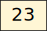
\includegraphics[scale=0.55]{Chapt_surrogates/figs/uqSample3}
		\caption{Run Samples}
		\label{fig.tut.sur.new.uq.sample3}
	\end{center}
\end{figure}

\subsection{Data Selection}

Initial and validation data can be specified by creating filters that specify subsets of flowsheet data. In this tutorial only initial data will be used. A filter must be created to separate the results of the single test run from the UQ samples.

\begin{enumerate}
	\setcounter{enumi}{23}
	\item Click on the \textbf{\underline{Surrogates}} button from the Home window. The surrogate tool displays \ref{fig.tut.sur.data}.
	\item Select ``ALAMO'' from the \textbf{\underline{Tool}} drop-down list.
	\item Click \textbf{\underline{Edit Filters}} in the \textbf{\underline{Flowsheet Results}} section to create a filter.
\end{enumerate} 
\begin{figure}[H]
	\begin{center}
		
\includegraphics[scale=0.55]{Chapt_surrogates/figs/data}
		\caption{Surrogate Data}
		\label{fig.tut.sur.data}
	\end{center}
\end{figure}

\begin{enumerate}
	\setcounter{enumi}{26}
	\item Figure \ref{fig.tut.sur.dataFilter} displays the Data Filter Editor. 
	\item Add the filter for initial data.
	\begin{enumerate}
		\item Click \bu{New Filter}, and enter ``Initial'' as the filter name.
		\item Click \bu{Add Rule}.
		\item In the ``Term 1'' column enter: set (no quotes).
		\item In the ``Term 2'' column enter: ``UQ\_Ensemble'' (with quotes).
		\item In the ``Operator'' column select ``=.''	
	\end{enumerate}
	\item Click \textbf{\underline{Done}}.
\end{enumerate}
\begin{figure}[H]
	\begin{center}
		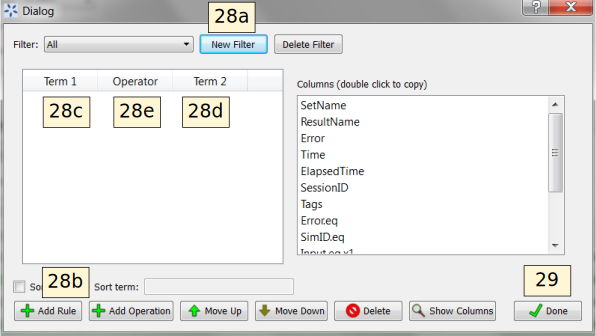
\includegraphics[scale=0.55]{Chapt_surrogates/figs/dataFilter}
		\caption{Data Filter Dialog}
		\label{fig.tut.sur.dataFilter}
	\end{center}
\end{figure}

\subsection{Variable Selection}
In this section, input and output variables need to be selected. Generally, any input variables that vary in the data set should be selected. However, in some cases, variables may be found to have no, or very little, effect on the outputs. Only the output variables of interest need to be selected. Note: Each output is independent from each other and for the model building, selecting one output is the same as selecting more.

\begin{enumerate}
	\setcounter{enumi}{29}
	\item Select the \textbf{\underline{Variable}s} tab (Figure \ref{fig.tut.sur.vaiables}).
	\item Select the checkbox for both input variables.
	\item Select the checkbox for both output variables.
\end{enumerate}
\begin{figure}[H]
	\begin{center}
		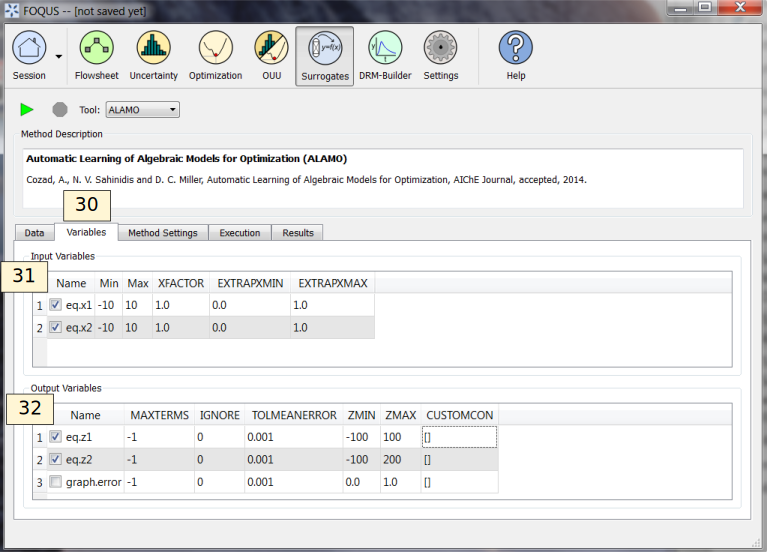
\includegraphics[scale=0.55]{Chapt_surrogates/figs/variables}
		\caption{Variable Selection}
		\label{fig.tut.sur.vaiables}
	\end{center}
\end{figure}

\subsection{Method Settings}
\label{tutorial.alamo.methodsettings}
The most important feature to generate "good" algebraic models is to configure the settings accordingly to the problem to be solved.  Each setting has a good description in FOQUS. The JSON parser is used to read method settings values. Strings must be contained in quotes. Lists have the following format: [element 1, element 2].

\begin{enumerate}
	\setcounter{enumi}{32}
	\item Click on the \textbf{\underline{Method Settings}} tab (see Figure \ref{fig.alamo.method.settigs}).
	\item Set the \textbf{\underline{FOQUS Model (for UQ)}} to ``ALAMO\_tutorial\_UQ.py.'' 
	\item Set the \textbf{\underline{FOQUS Model (for Flowsheet)}} to ``ALAMO\_tutorial\_FS.py''
	\item Set \textbf{\underline{Initial Data Filter}} to ``Initial.''
	\item Set \textbf{\underline{SAMPLER}} to select the adaptive sampling method: ``None'' ``Random'' or ``SNOBFIT.'' Use ``None'' in this tutorial.
	\item Set \textbf{\underline{MONOMIALPOWER}} to select the single variable term powers to [1,2,3].
	\item Set \textbf{\underline{MULTI2POWER}} to select the two variable term powers to [1].
	\item Select functions to be considered as basis functions (\textbf{\underline{EXPFCNS}}, \textbf{\underline{LOGFCNS}}, \textbf{\underline{SINFCNS}}, \textbf{\underline{COSFCNS}}).
	\item Leave the rest of settings as default (see Table \ref{tutorial.alamo.table}).
	\item Save this FOQUS session for use in the ACOSSO and BSS-ANOVA tutorials.
\end{enumerate}
\begin{figure}[H]
	\begin{center}
		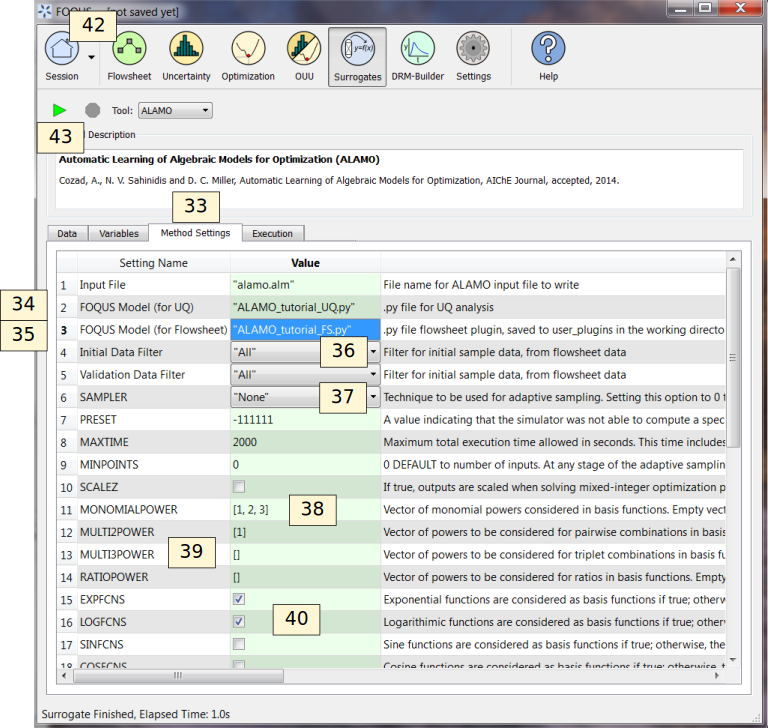
\includegraphics[scale=0.55]{Chapt_surrogates/figs/alamo_settings}
		\caption{ALAMO Method Settings}
		\label{fig.alamo.method.settigs}
	\end{center}
\end{figure}

\subsection{Execution}

\begin{enumerate}
	\setcounter{enumi}{42}
	\item Click the \bu{Run} icon at the top of the window.
	\item The ALAMO \bu{Execution} tab starts displaying execution file path, sub-directories, input files, and output files.
\begin{enumerate}
	\item ALAMO version.
	\item License Information.
	\item Step 0 displays the data set to be used by ALAMO.
	\item Step 1 displays the modeler used by ALAMO to generate the algebraic model.
	\item Once the surrogate model has finished, the equations are displayed in the execution window. It may be necessary to scroll up a little. The result is shown in Figure \ref{fig.alamo.res}.
	\item Finally, the statistics display the quality metrics of the models generated.
\end{enumerate}
\end{enumerate}

\begin{figure}[H]
	\begin{center}
		\includegraphics[scale=0.4]{Chapt_surrogates/figs/alamo_exec}
		\caption{ALAMO Execution}
		\label{fig.alamo.res}
	\end{center}
\end{figure}

\subsection{Results}
	The results are exported as a PSUADE driver file that can be used perform UQ analysis of the models, and a FOQUS Python plugin model that allows it to be used in a FOQUS flowsheet. The equations can also be viewed in the results section.
	
	See tutorial Section \ref{tutorial.surrogate.uq} and \ref{tutorial.surrogate.fs} for information about analyzing the model with the UQ tools or running the model on the flowsheet.
	
	As mentioned in section \ref{tutorial.alamo.methodsettings} the method settings are very important. A brief description and hints are included in Table \ref{tutorial.alamo.table}.

\begin{center}

\begin{longtable}{|p{.30\textwidth}|p{.70\textwidth} |}
\caption{ALAMO Method Settings}
\label{tutorial.alamo.table} \\

		\hline
			\textbf{Method Settings} & \textbf{Description} \\		\hline
			Initial Data Filter & Filter to be applied to the initial data set. Data filters help the user to generate models based on specific data for each variable.  \\	\hline
			Validation Data filter & Data set used to compute model errors at the validation phase. The number of data points in a preexisting validation data set can be specified by the user.\\	\hline
			SAMPLER & Adaptative sampling method to be used. Options: "None", "Random" and "SNOBFIT". Adaptive sampling method to be used by ALAMO when more sampling points are needed by the model. If \bu{Random} is used a simulator must be provided by the user. If \bu{SNOBFIT} is used a simulator must be provided by the user and MATLAB must be installed.\\	\hline
			MAXTIME& Maximum execution time in seconds. This time includes all the steps on the algorithm, if simulations are needed they run in this time.\\	\hline
			MINPOINTS& Convergence is assessed only if the simulator is able to compute the output variables for at least MINPOINTS of the data set. A reduced number of MINPOINTS may reduce the computational time to get a model, but also reduces the accuracy of the model. MINPOINTS must be a positive integer. \\ \hline
			PRESET&Value to be used if the simulator fails. This value must be carefully chosen to be an otherwise not realizable value for the output variables.\\ \hline
			MONOMIALPOWERS &  Vector of monomial powers to be considered as basis functions, use empty vector for none []. Exponential terms allowed in the algebraic model.  i.e., if selecting [1,2] the model considers x1 and x1**2 as basis functions. \\ \hline
			MULTI2POWER & Vector of pairwise combination of powers to be considered as basis functions. Pairwise combination of powers allowed in the algebraic model. i.e., [1,2] allows terms like x1*x2 in the algebraic model.\\ \hline
			MULTI3POWER & Vector of three variables combinations of powers to be considered as basis functions. \\ \hline
			\raggedright{EXPFCNS, LOGFCNS, SINFCNS, COSFCNS functions}& Use or not of exp, log, sin, and cos functions as basis functions in the model. \\ \hline
			RATIOPOWER& Vector of ratio combinations of powers to be considered in the basis functions. Ratio combinations of powers are [empty as default].\\ \hline
			Radial Basis Functions& Radial basis functions centered around the data set provided by the user. These functions are Gaussian and are deactivated if their textual representation requires more than 128 characters (in the case of too many input variables and/or datapoints). \\ \hline
			RBF parameter&Constant penalty used in the Gaussian radial basis functions.  \\ \hline
			Modeler & Fitness metric to be used for model building. Options: BIC (Bayesian Information Criterion), Mallow's Cp, AICc (Corrected Akaike's Information Criterio), HQC (Hannan-Quinn Information Criterion), MSE (Mean Square Error), and Convex Penalty. \\ \hline
			ConvPen& Convex penalty term. Used if Convex Penalty is selected. \\ \hline
			Regularizer & Regularization method is used to reduce the number of potential basis functions before the optimization.\\ \hline 
			Tolrelmetric & Convergence tolerance for the chosen fitness metric is needed to terminate the algorithm. \\ \hline
			ScaleZ&If used, the variables are scaled prior to the optimization problem is solved. The problem is solved using a mathematical programming solver. Usually, scaling the variables may help the optimization procedure.\\ \hline
			GAMS&GAMS is the software used to solve the optimization problems. The executable path is expected or the user must declare GAMS.exe in the environment path.\\ \hline
			GAMS Solver&Solver to be used by GAMS to solve the optimization problems. Mixed integer quadratic programming solver is expected like BARON (other solvers can be used).\\ \hline
			MIPOPTCR & Relative convergence tolerance for the optimization problems solved in GAMS. The optimization problem is solved when the optcr is reached. 5 to 1 \% is expected (0.005 to 0.001).\\ \hline
			MIPOPTCA & Absolute convergence tolerance for mixed-integer optimization problems. This must be a nonnegative scalar. \\ \hline
			Linear error & If true, a linear objective function is used when solving the mixed integer optimization problems; otherwise, a quadratic objective function is used. \\ \hline
			\raggedright{Constraint Regression (CONREG)} & Specify whether constraint regression is used or not, if true bounds on output variables are enforced. \\ \hline
			CRNCUSTOM & If true, Custom constraints are entered in the Variable tab.\\ \hline
			CRNINITIAL& Number of random bounding points at which constraints are sampled initially (must be a nonnegative integer). \\ \hline
			CRNMAXITER & Maximum allowed constrained regressions iterations. Constraints are enforced on additional points during each iteration (must be positive integer). \\ \hline
			CRNVIOL & Number of bounding points added per round per bound in each iteration (must be positive integer). \\ \hline
			CRNTRIALS&Number of random trial bounding points per round of constrained regression (must be a positive integer). \\ \hline
			CUSTOMBAS&A list of user-supplied custom basis functions can be provided by the user. The parser is not case sensitive and allows for any Fortran functional expression in terms of the XLABELS (symbol \^{} may be used to denote power). \\ \hline
			
%		\end{tabularx}
%	\end{center}

\end{longtable}	
\end{center}	

\section{Tutorial -- ACOSSO}
\label{(sec.surrogate.acosso)}

This tutorial covers the ACOSSO surrogate modeling method. The Adaptive
COmponent Selection and Shrinkage Operator (ACOSSO) surface approximation
was developed under the Smoothing Spline Analysis of Variance (SS-ANOVA)
modeling framework \citep{Storlie_2011}. As it is a smoothing type method,
ACOSSO works best when the underlying function is somewhat smooth. For
functions which are known to have sharp changes or peaks, etc., other
methods may be more appropriate. Since it implicitly performs variable
selection, ACOSSO can also work well when there are a large number of input
variables. 
The ACOSSO procedure also allows for
categorical inputs \citep{Storlie_2013}.
 
This tutorial uses the same flowsheet and sample setup as the ALAMO
tutorial in Section \ref{sec.surrogate.alamo}. The statistics software
``R'' is also required to use ACOSSO and BSS-ANOVA. Before starting this
tutorial, you will need to install R version 3.1 or later (see \href{http://cran.r-project.org/}{\textcolor{blue}{https://cran.r-project.org/}}). 

Once R is installed, you will need to install the ``quadprog''
package. ACOSSO requires this package for solving quadratic
programming problems. You will only need to perform this step once. 

\begin{enumerate}
\item{Start R. In Windows, this must be done with administrative
  privileges.  Either run this from an administrator account, or
  right-click ``R x64 3.1.2'' and click ``Run with administrator'' and type
  in administrator credentials.}
\item{Inside the R console, type:
   \begin{itemize} 
   \item \tt install.packages('quadprog')
   \item \tt library(quadprog)
   \item \tt q()
  \end{itemize}
The first line installs the package. If prompted for a CRAN mirror, select
the one closest to you geographically. The second line loads the
package. The last line quits R. If prompted to save workspace image, choose
`y'.}
\end{enumerate}

Once you have done these steps, ACOSSO is ready to be invoked inside FOQUS.

\begin{enumerate}
	\item{Set the path to the RScript executable.}
		\begin{enumerate}
			\item Click the \bu{Settings} button in the Home window.
			\item Change the RScript path if necessary. The \bu{Browse} button
           opens a file browser that can be used to set the path.
		\end{enumerate}
	\item Complete the ALAMO tutorial in Section \ref{sec.surrogate.alamo} through Step 32, or load the FOQUS session saved after completing the ALAMO tutorial.
	\item Click the \bu{Surrogates} button in the Home window (Figure \ref{fig.acosso.settings}).
	\item Select ``ACOSSO'' in the \bu{Tool} drop-down list.
	\item Select the \bu{Method Settings} tab.
	\item Set ``Data Filter'' to ``Initial.''
	\item Set ``Use Flowsheet Data'' to ``Yes.''
	\item Set ``FOQUS Model (for UQ)'' to ``ACOSSO\_Tutorial\_UQ.py.''
	\item Set ``FOQUS Model (for Flowsheet)'' to ``ACOSSO\_Tutorial\_FS.py.''
	\item Click the \bu{Run} icon (Figure \ref{fig.acosso.settings}).
\end{enumerate}

\begin{figure}[H]
	\begin{center}
		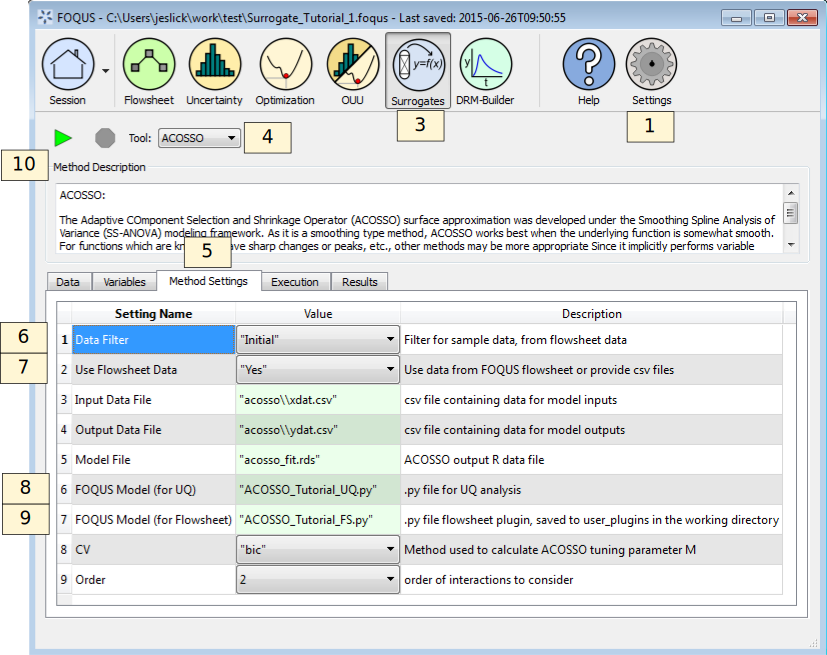
\includegraphics[scale=0.55]{Chapt_surrogates/figs/acosso_settings}
		\caption{ACOSSO Session Set Up}
		\label{fig.acosso.settings}
	\end{center}
\end{figure}

\begin{enumerate}
	\setcounter{enumi}{10}
	\item The execution window will automatically display. While ACOSSO is
     running, the execution window may show warnings, but this is normal.
	\item When the run completes, a UQ driver file is created, allowing the
     ACOSSO surrogate to be used as a user-defined response surface in UQ
     analyses. (See Section \ref{tutorial.surrogate.uq}.)
	\item ACOSSO also produces a flowsheet plugin; however.
\end{enumerate}



\section{Tutorial -- BSS-ANOVA}
\label{(sec.surrogate.bssanova)}

This tutorial covers the BSS-ANOVA surrogate modeling method.  The Bayesian
Smoothing Spline ANOVA (BSS-ANOVA) is essentially a Bayesian version of
ACOSSO \citep{Reich_2009}.  It is Gaussian Process (GP) model with a
non-conventional covariance function that borrows its form from SS-ANOVA.
It tackles the high dimensionality (of inputs) on two fronts: (1) variable
selection to eliminate uninformative variables from the model and (2)
restricting the level of interactions involved among the variables in the
model. This is done through a fully Bayesian approach which can also allow
for categorical input variables with relative ease. Since it is closely
related to ACOSSO, it generally works well in similar settings as
ACOSSO. The BSS-ANOVA procedure also allows for categorical inputs
\citep{Storlie_2013}. In this current implementation, BSS-ANOVA is more
computationally intensive than ACOSSO, so ACOSSO is preferred for faster
surrogate generation. 

This tutorial uses the same flowsheet and sample setup as the ALAMO
tutorial in Section \ref{sec.surrogate.alamo}. The statistics software
``R'' is also required to use ACOSSO and BSS-ANOVA. Before starting this
tutorial, you will need to install R version 3.1 or later (see \href{https://cran.r-project.org/}{\textcolor{blue}{http://cran.r-project.org/}}).

\begin{enumerate}
	\item{Set the path to the RScript executable.}
		\begin{enumerate}
			\item Click the \bu{Settings} button from the Home window.
			\item Change the RScript path if necessary.  The \bu{Browse} button opens a file browser that can be used to set the path.
		\end{enumerate}
	\item Complete the ALAMO tutorial in Section \ref{sec.surrogate.alamo} through Step 32, or load the FOQUS session saved after completing the ALAMO tutorial.
	\item Click the \bu{Surrogates} button from the Home window (Figure \ref{fig.bssanova.settings}).
	\item Select ``BSS-ANOVA'' in the \bu{Tool} drop-down list.
	\item Select the \bu{Method Settings} tab.
	\item Set ``Data Filter'' to ``Initial.''
	\item Set ``Use Flowsheet Data'' to ``Yes.''
	\item Set ``FOQUS Model (for UQ)'' to ``bssanova\_tutorial\_uq.py.''
	\item Set ``FOQUS Model (for Flowsheet)'' to ``bssanova\_tutorial\_fs.py.''
	\item Click the \bu{Run} icon (Figure \ref{fig.bssanova.settings}).
\end{enumerate}

\begin{figure}[H]
	\begin{center}
		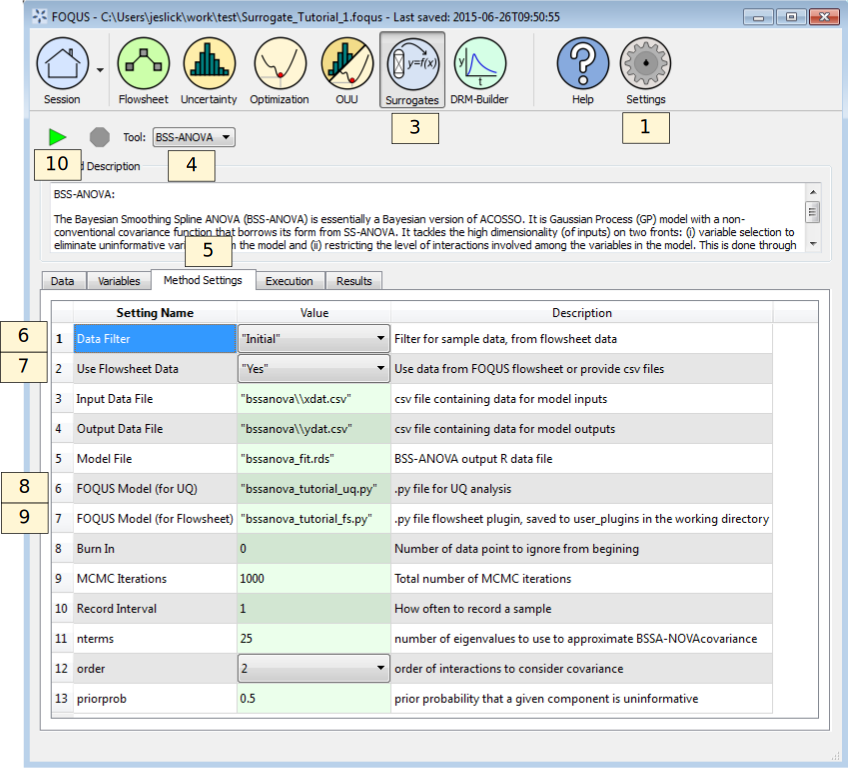
\includegraphics[scale=0.55]{Chapt_surrogates/figs/bssanova_settings}
		\caption{BSS-ANOVA Session Set Up}
		\label{fig.bssanova.settings}
	\end{center}
\end{figure}

\begin{enumerate}
   \setcounter{enumi}{10}
   \item The execution window will automatically display. While BSS-ANOVA is
     running, the execution window may show warnings, but this is normal.
   \item When the run completes, a UQ driver file is created, allowing the
     BSS-ANOVA surrogate to be used as a user-defined response surface in UQ
     analyses. (See Section \ref{tutorial.surrogate.uq}.)
   \item BSS-ANOVA also produces a flowsheet plugin.
\end{enumerate}


\section{Tutorial -- iREVEAL} 
The iREVEAL documentation is currently separate, but will be merged in the next release. The iREVEAL user's manual is included in the FOQUS installation.  There is a link to the manual in the Windows start menu under CCSI Tools\bs FOQUS.

\section{Tutorial -- Surrogates with UQ Tools}
\label{tutorial.surrogate.uq}

For the purpose of this tutorial, we will use ACOSSO to demonstrate the use
of a surrogate within the UQ module. The steps are the same regardless of
the surrogate tool chosen.

To perform the UQ analysis, Python is required for use the ``User Regression'' response surface that will be used.  Before starting this tutorial, you will need to install Python 2.7.x (not Python 3). (See \href{https://www.python.org/downloads/}{\textcolor{blue}{https://www.python.org/downloads/}}). In addition, if *.py files have been re-associated with other executables (e.g. editors), please change the association back to python.exe. 


\begin{enumerate}
\item{Load a fresh session by clicking the \bu{Session} button from the Home window. Select \textbf{\underline{Open Session}} and then navigate to the ``examples/UQ''
  directory. Select ``Rosenbrock\_no\_vectors.foqus.'' This will load a
  session with a simple flowsheet containing a single node.}
\item{Click \bu{Settings} and ensure that (1) FOQUS Flowsheet Run Method is
  set to ``Local'', and that (2) proper paths are set for PSUADE and RScript.} 
\item{Train an ACOSSO surrogate of this node by clicking the
  \bu{Surrogates} button from the Home window.
\begin{enumerate}
\item{Click \bu{Add Samples} and select ``Use Flowsheet''. This will
  display the \bu{Simulation Ensemble Setup} dialog.}
\item{Within this dialog, ensure all variables are set to ``Variable''
  type in the \bu{Distributions} tab. In the \bu{Sampling scheme} tab,
  select ``Monte Carlo'' as your sampling scheme, set the number of
  samples to 100, and then click \bu{Generate Samples} to generate the
  set of input values. Click \bu{Done} to return to the Surrogates screen.}
\item{Once sample generation completes, click the \bu{Uncertainty} button from the Home window.}
\item{Click the \bu{Launch}	button to generate the samples.}
\item{Click the \bu{Surrogates} button from the Home window. The \bu{Data} tab of the Surrogates
  screen should now displays a \bu{Flowsheet Results} table that is populated with
  the values of the new input samples.}
\item{From the \bu{Variables} tab, select all of the checkboxes. (There should
  be six checkboxes for input variables and one checkbox for output variable.) 
  Here, you are defining the inputs and outputs for your surrogate function.}
\item{From the \bu{Method Settings} tab, note the name of the file next to
  ``FOQUS Model (for UQ)''. This will be the name of the UQ driver file
  that contains the Python code that implements the surrogate function.}
\item{On top of this screen, select ``ACOSSO'' as your surrogate tool from the \textbf{\underline{Tool}} drop-down list and then click on the green arrow to start training the surrogate.}
\item{Once complete, a popup window will display, reminding you of the
  location of the drive file. Note the location as you will need this
  information later inside the UQ module.} 
\end{enumerate}
}
\item{Perform a response-surface-based uncertainty analysis by clicking the 
  \bu{Uncertainty} button from the Home window.
\begin{enumerate}
\item{In the \bu{Uncertainty Quantification Simulation Ensembles} table. A row corresponding to the ensemble that was just
  generated for surrogate training should be displayed. This same ensemble can be used or
  a new one can be created to be used as the test data set for analysis. 
  In the row corresponding to the ensemble
  to be analyzed, click the \bu{Analyze} button to proceed. This
  action will bring up an analysis dialog.} 
\item{Within this analysis dialog, navigate to ``Analysis'' section. For
  Step 1, select ``Response Surface''. For Step 3, select ``User
  Regression'' in the first drop-down list. Lastly, for ``User Regression File'',
  browse to the same location as the UQ driver file that was
  generated within the Surrogates module. (This is the same location that
  was previously noted from the popup message.) 
  At this point, your surrogate function is now set up as a user-defined
  response surface and all response-surface-based UQ analyses are accessible.}
\item{Click \bu{Validate} (Step 4) to perform response surface validation. Once
  complete, a figure with cross-validation results will be displayed: 
  a histogram of errors to the left and a plot of predicted values versus
  actual values to the right. For more information, refer to the UQ
  Tutorial in Section \ref{tutorial.uq.rs}.}
\item{Once a ``Response Surface'' has been validated, other UQ analysis options
  are available. Choose ``Uncertainty Analysis'' in Step 5 and click
  \bu{Analyze} to perform uncertainty analysis using your ACOSSO surrogate.}
\end{enumerate}
}
\end{enumerate}

During validation, if the error, ``RSAnalyzer: RSTest\_hs.m does
not exist.'' displays, this is likely caused by incompatibility with the surrogate
and the test data. An example scenario might be your test data has six
inputs, but your surrogate assumes five inputs. This is easily fixed by
returning to the Surrogates screen, clicking on the \bu{Variables}
tab, and making sure the appropriate selections are made (i.e., check off six
inputs instead of just five).

\section{Tutorial -- Surrogates with the Flowsheet}\label{tutorial.surrogate.fs}

This section provides a brief tutorial for using the flowsheet plugin models generated by surrogate modeling methods. In the next FOQUS release all surrogate modeling methods will produce a model that can be run in a FOQUS flowsheet. \textbf{Currently iREVEAL does not produce a flowsheet model.}

\textbf{Before doing this tutorial complete the ALAMO tutorial in Section \ref{sec.surrogate.alamo}.}

\begin{enumerate}
	\item Open FOQUS.  If FOQUS has not been closed since completing the ALAMO tutorial, close it and reopen it. There is a known issue where existing flowsheet model plugins may not update until FOQUS is restarted.
	\item Enter ``FS\_Plugin\_Tutorial'' as the Session Name.
	\item Click the \bu{Flowsheet} button from the Home window.
	\item Click the \bu{Add Node} icon in the left toolbar (see Figure \ref{fig.pg.tut1}).
	\item Click a location for the node in the Flowsheet area.
	\item Enter ``model'' for the node name (without quotes).
	\item Click the \bu{Node Editor} icon in the left toolbar (see Figure \ref{fig.pg.tut1}).
	\item In the \textbf{\underline{Node Editor}}, select ``Plugin'' from the Model \textbf{\underline{Type}} drop-down list. 
	\item Select ``ALAMO\_Tutorial\_FS'' from the \textbf{\underline{Model}} drop-down list. 
	\item Set the \textbf{\underline{Value}} of the \textbf{\underline{Input Variables}} ``eq.x1'' to 2.
	\item Set the \textbf{\underline{Value}} of the \textbf{\underline{Input Variables}} ``eq.x2'' to 3.
	\item Click the \bu{Run} icon in the left toolbar (see Figure \ref{fig.pg.tut1}).
	\item Wait for the Flowsheet evaluation to complete. It should finish successfully.
	\item Check the value of the \textbf{\underline{Output Variables}}; the approximate values should be z1 = 5 and z2 = 13.
\end{enumerate}

\begin{figure}[H]
	\begin{center}
		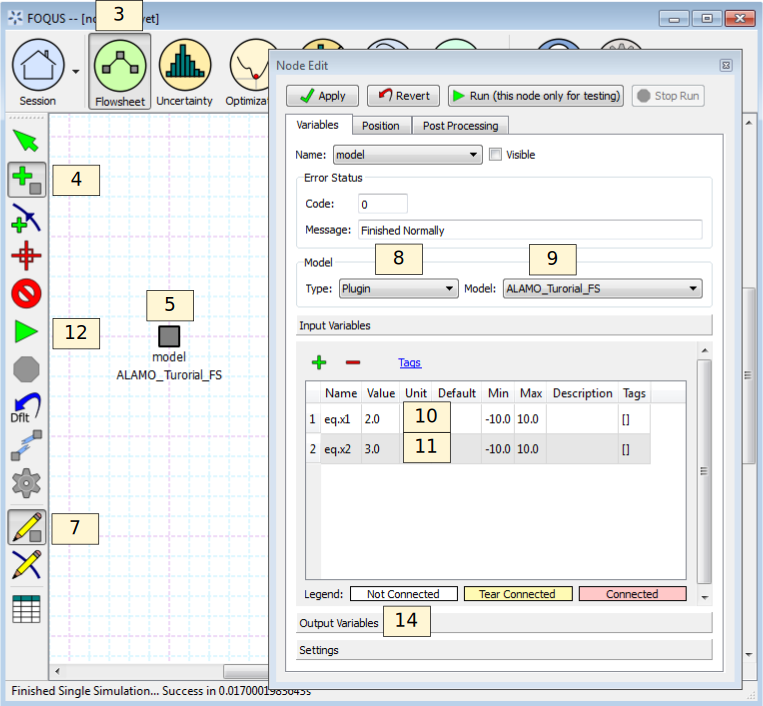
\includegraphics[scale=0.55]{Chapt_surrogates/figs/fs_plugin}
		\caption{Plugin Flowsheet}
		\label{fig.pg.tut1}
	\end{center}
\end{figure}




	

\chapter{Surrogate Models}\label{chpt.surrogates}

\section{D-RM (Dynamic Reduced Models) Builder}\label{sec.overview.drm}

The Dynamic Reduced Model (D-RM) Builder is a software tool used to generate data-driven dynamic reduced models from high-fidelity dynamic models consisting of differential and algebraic equations (DAEs).  DAE-based models are usually computationally intensive to solve, especially when stiff DAEs are involved.  For instance, the sorbent-based bubbling fluidized bed CO$_2$ adsorber-reactor model contains over 20,000 DAEs and very small time steps ($<$0.001 second) have to be used to solve the stiff equations in the rigorous model.  The D-RMs generated by the D-RM Builder enable much faster computation of the system responses (up to several orders of magnitude faster), which enable the development of an advanced process control framework and the integration of the dynamic models within a large-scale dynamic simulation.

\subsection{Motivating Example}

The solid-sorbent-based bubbling fluidized bed CO$_2$ adsorber-reactor for the post-combustion carbon capture is a good example to which the D-RM Builder tool can be applied.  The dynamics of the adsorber-reactor was modeled by a CCSI team using Aspen Custom Modeler (ACM).  The high-fidelity dynamic model of the twin-bed adsorber-reactor contains over 20,000 equations.  The feed streams include CO$_2$-containing flue gas, solid sorbent, and multiple cooling water streams.  Since some equations are very stiff, a minimum integration time step of 0.001 second has to be used.  As a result, the computer CPU time required to calculate the response of the system over a period of operating time is much longer than the real operating time, especially when there is a change in model inputs (step or ramp change).  The data-driven D-RM can be generated by fitting the system outputs in response to the changes of system inputs through certain plant identification models.  The response of the system to the input changes can be simulated by the ACM model.  The D-RM Builder is provided for a user to configure the input and output variables of interest, prepare a sequence of step changes of input variables, launch ACM simulations, generate a D-RM, and export the D-RM in a form of a MATLAB function file (.m file), which can be called by MATLAB to calculate the system response given the model inputs with a CPU execution time a few orders of magnitude shorter than that required by the ACM model.  The speedup in CPU time enables the implementation of advanced process control (APC) systems.

\subsection{Features List}

The D-RM Builder is an application embedded in the graphic user interface (GUI) of FOQUS.  Data-driven D-RMs can be generated by the D-RM Builder based on a set of high-fidelity model outputs in response to a sequence of input changes within a range of operating conditions.  The D-RM Builder can read the input and output variables pre-configured through SinterConfigGUI application, which is also a part of the FOQUS package.  Through the D-RM Builder GUI, a user can select a set of the pre-configured input variables, specify their lower and upper limits, and prepare a sequence of step changes or ramp changes based on the Latin Hypercube Sampling (LHS) method with desired durations of the step changes to excite the system in a range of frequencies.  The simulations of high-fidelity models, currently implemented for ACM only, can be launched directly in the D-RM Builder through ConsoleSinter, which is also a part of the FOQUS package.  The simulation results can be used to generate the D-RMs.  A separate set of step-change sequence can also be generated and its response be simulated by the ACM model and predicted by the D-RM for validation purpose.  The generated D-RMs and the user inputs for case setup and configuration can be saved in a text file in JSON format with extension ``drmb''.  Once a case file is saved, the user can copy the file to a different directory or to a different computer where the D-RM Builder is installed and open the file later to continue the D-RM building process or visualize the properties of the generated D-RMs.  A D-RM Builder project could also be a subproject of a FOQUS project and saved as a part of FOQUS session.  When a saved FOQUS session file is opened, the D-RM Builder subproject is also opened.

Two types of D-RMs are supported in the current version including the Decoupled A-B Net (DABNet) model \cite{Sentoni_1998}, and the Nonlinear Auto-regressive Moving Average (NARMA) model \cite{Narendra_1997}.  Different building options are provided for the user to choose from including input delays, two-pole Laugerre formulation of DABNet model, and optimization of model parameters.  Both D-RM model types require the training of artificial neural networks (ANNs).  Two ANN training methods, back propagation (BP) and interior point optimization (IPOPT), are provided.  The generated D-RM can be validated by performing another set of high-fidelity model simulations with a different input change sequence and comparing the response to that predicted by the generated D-RMs.  The response calculated by the high-fidelity model and that by the D-RM can be displayed through the D-RM Builder$\text{'}$s GUI.  The accuracy of the generated D-RM can be visualized by comparing the D-RM predictions to the corresponding ACM predictions, including the relative errors and the coefficient of determination R$^2$.  For the state-space based DABNet model, Uncertainty Quantification (UQ) analysis can be performed on the validation data using Unscented Kalman Filter (UKF), providing the covariance matrices of state-space and output variables.  The messages of the model building process including command sequence are displayed in the main text window of the D-RM Builder, which can be saved to a log file for future reference.  The internal parameters of the generated D-RM can be exported to a MATLAB script file, which can be run in MATLAB to initialize a D-RM object instantiated from a MATLAB class.  The results of the high-fidelity model simulations and D-RM predictions for both the training and the validation input sequences can also be exported to text files in comma-separated value (CSV) format, which can be opened by Microsoft® Excel®.

Along with the D-RM Builder application, several MATLAB files are also provided as part of the software tool.  These files define the MATLAB classes that can be used to create the D-RM objects in the MATLAB workspace given the D-RM files exported from the D-RM Builder.  The functions in the D-RM objects can be called to perform dynamic simulations.

\section{Tutorial -- ALAMO}
\label{sec.surrogate.alamo}
This tutorial focuses on the use of the ALAMO tool for building algebraic surrogate models. ALAMO builds simplified algebraic models, which are particularly well suited for rigorous equation oriented optimization. To keep the execution of this tutorial fast, a toy problem is used. In this case study the flowsheet calculations and sample generation are done within FOQUS, alternatively, the user can provide a simulation model such as: Excel, Aspen plus, Aspen custom modeler, etc. 

Note: Before starting this tutorial the ALAMO product must be downloaded from the products page on the CCSI website. The path for the ALAMO executable file must be set in FOQUS settings (see Section \ref{section.settings}).

\subsection{Flowsheet Setup}

\begin{enumerate}
	\item Open FOQUS.
	\item Name the session ``Surrogate\_Tutorial\_1'' (Figure \ref{fig.tut.sur.session}).
\end{enumerate}

\begin{figure}[H]
	\begin{center}
		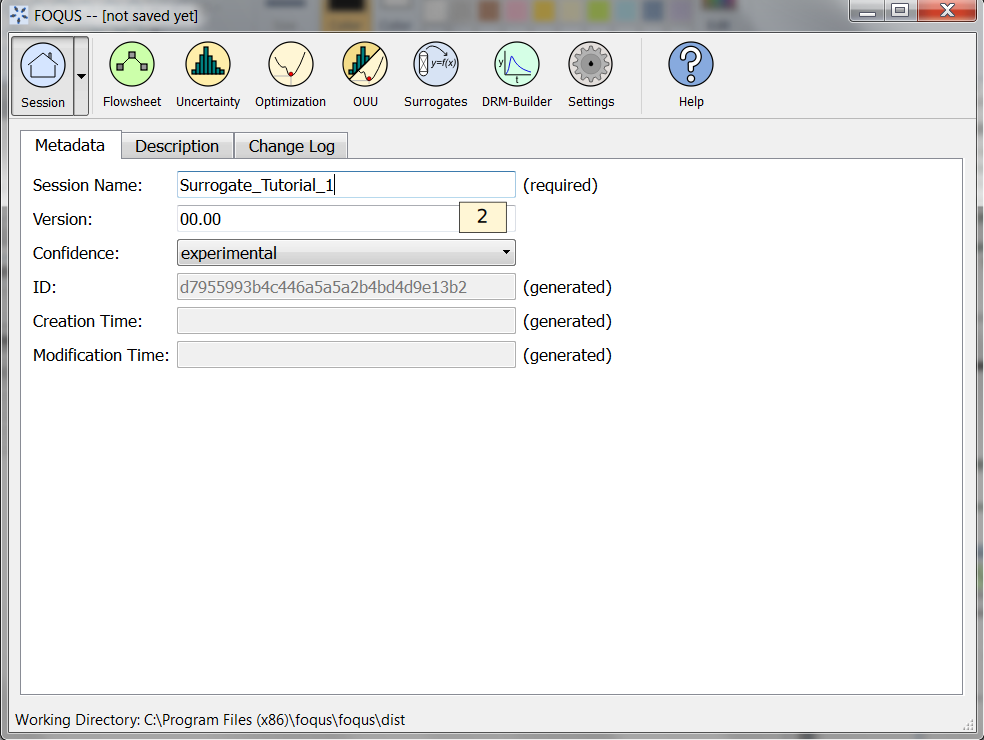
\includegraphics[scale=0.55]{Chapt_surrogates/figs/session1}
		\caption{Session Set Up}
		\label{fig.tut.sur.session}
	\end{center}
\end{figure}

\begin{enumerate}
	\setcounter{enumi}{2}
	\item Navigate to the Flowsheet Editor (Figure \ref{fig.tut.sur.flowsheet}).
	\item Add a Flowsheet Node named ``eq.''
	\item Display the Node Editor by clicking the \textbf{\underline{Node Editor}} toggle button.
\end{enumerate}
\begin{figure}[H]
	\begin{center}
		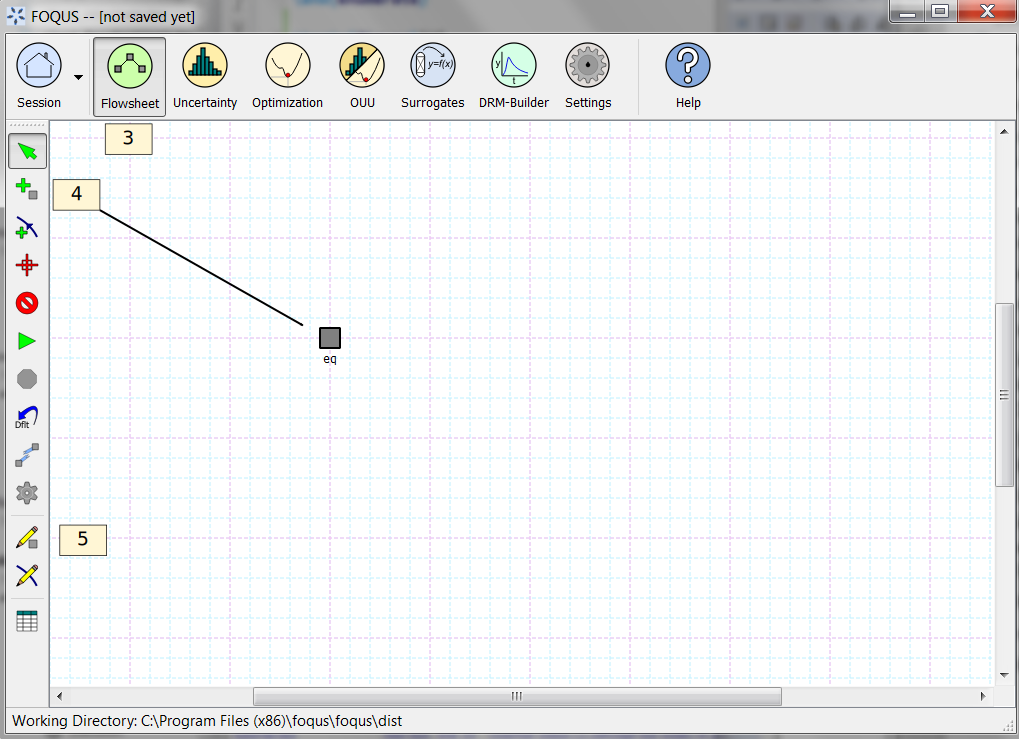
\includegraphics[scale=0.55]{Chapt_surrogates/figs/flowsheet}
		\caption{Flowsheet Setup}
		\label{fig.tut.sur.flowsheet}
	\end{center}
\end{figure}
The \textbf{\underline{Node Editor}} displays (Figure \ref{fig.tut.sur.nodeEdit.Input}).  The first step to setting up the node for this problem is to add input and output variables to the node.
%Does more detail need added to #9 below since the figure shows x1 and x2 in the Input Variables menu. Does the user need to know to click on Output Variables to open the Output Variables screen, then enter z1 and z2 under the Name column?
\begin{enumerate}
	\setcounter{enumi}{5}
	\item If the input variables table is not displayed as shown in Figure \ref{fig.tut.sur.nodeEdit.Input}, click the \textbf{\underline{Variables}} tab and then click the \textbf{\underline{Input Variables}} toolbox section.
	\item Add the variables ``x1'' and ``x2'' by clicking the \textbf{\underline{Add}} icon (+) above the input table.
	\item Edit the \textbf{\underline{Min/Max}} value for both variables to be ``-10.0'' and ``10.0.''
	\item Add two output variables ``z1'' and ``z2.''
\end{enumerate}
\begin{figure}[H]
	\begin{center}
		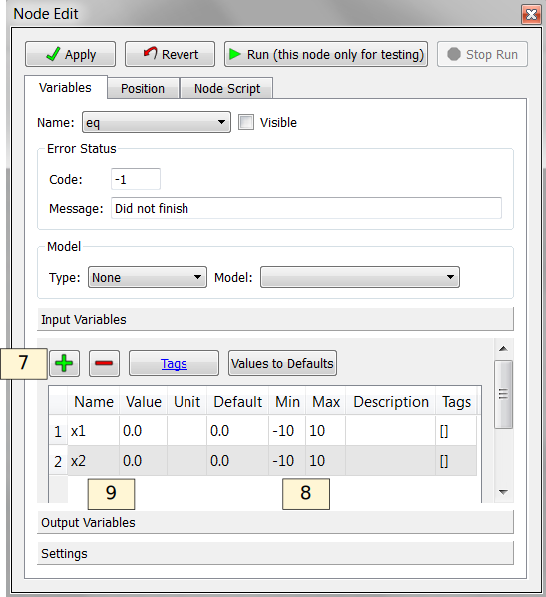
\includegraphics[scale=0.55]{Chapt_surrogates/figs/nodeInput}
		\caption{Node Variables}
		\label{fig.tut.sur.nodeEdit.Input}
	\end{center}
\end{figure}
To keep the execution time short, the node will not be assigned to a simulation model and calculations are performed directly in FOQUS.  
\begin{enumerate}
	\setcounter{enumi}{9}
	\item Click on the \textbf{\underline{Node Script}} tab in the Node Editor to enter the test equation (this step replaces the use of a simulator).
	\item Enter the following equations (Figure \ref{fig.tut.sur.nodeEdit.eq}):
	\begin{verbatim}
		f["z1"] = x["x1"] + x["x2"]
		f["z2"] = x["x1"]**2 + x["x2"]**2
	\end{verbatim}
	The node script calculations are written in Python. The dictionary ``f'' stores output values while the dictionary ``x'' stores input values.

\begin{figure}[H]
	\begin{center}
		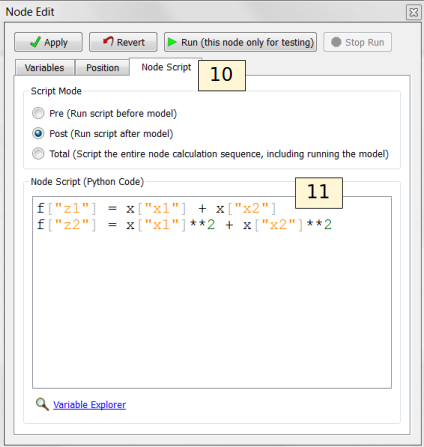
\includegraphics[scale=0.55]{Chapt_surrogates/figs/nodeEq}
		\caption{Node Script}
		\label{fig.tut.sur.nodeEdit.eq}
	\end{center}
\end{figure}

	\item Test the model by running the flowsheet with the value ``2'' for ``x1'' and ``x2.'' After running, the output variables should have the values ``4.0'' for ``z1'' and ``8.0'' for ``z2.''
\end{enumerate}


\subsection{Creating Initial Samples}

There are two ways to start an ALAMO run: (1) generate a set of initial data, (2) use ALAMO's adaptive sampling with no initial data and let ALAMO generates its own samples. Adaptive sampling can be used with initial data to generate more points if needed. In this case, initial data is provided and adaptive sampling is used.

\begin{enumerate}
	\setcounter{enumi}{12}
	\item Select the UQ tool by clicking on the \textbf{\underline{Uncertainty}} button on the Home window (Figure \ref{fig.tut.sur.new.uq.ens}).
	\item Click the \textbf{\underline{Add New}} button.
	\item The \textbf{\underline{Add New Ensemble - Model Selection}} dialog will appear. Click \textbf{\underline{OK}} to set up the sampling scheme.
\end{enumerate}
\begin{figure}[H]
	\begin{center}
		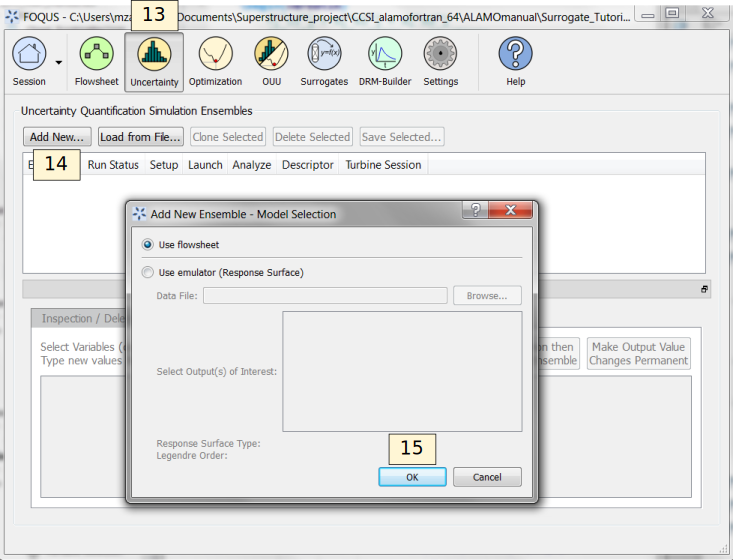
\includegraphics[scale=0.55]{Chapt_surrogates/figs/uqNewEns}
		\caption{Add a New Sample Ensemble}
		\label{fig.tut.sur.new.uq.ens}
	\end{center}
\end{figure}
\begin{enumerate}
	\setcounter{enumi}{15}
	\item The sample ensemble setup dialog displays (Figure \ref{fig.tut.sur.new.uq.sample1}).  Select \textbf{\underline{Choose sampling scheme}}. 
	\item Click the \textbf{\underline{All Variable}} button.
	\item Select the \textbf{\underline{Sampling scheme}} tab.
\end{enumerate}
\begin{figure}[H]
	\begin{center}
		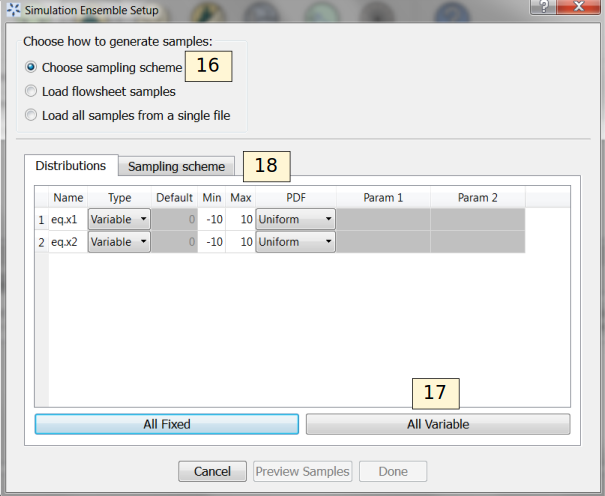
\includegraphics[scale=0.55]{Chapt_surrogates/figs/uqSample1}
		\caption{Sample Distributions}
		\label{fig.tut.sur.new.uq.sample1}
	\end{center}
\end{figure}
\begin{enumerate}
	\setcounter{enumi}{18}
	\item The \textbf{\underline{Sampling schem}e} dialog should display (Figure \ref{fig.tut.sur.new.uq.sample2}). Select ``Latin Hypercube'' from the list.
	\item Set the \textbf{\underline{\# of samples}} to ``10.''
	\item Click \textbf{\underline{Generate Samples}}.
	\item Click \textbf{\underline{Done}}.
\end{enumerate}
\begin{figure}[H]
	\begin{center}
		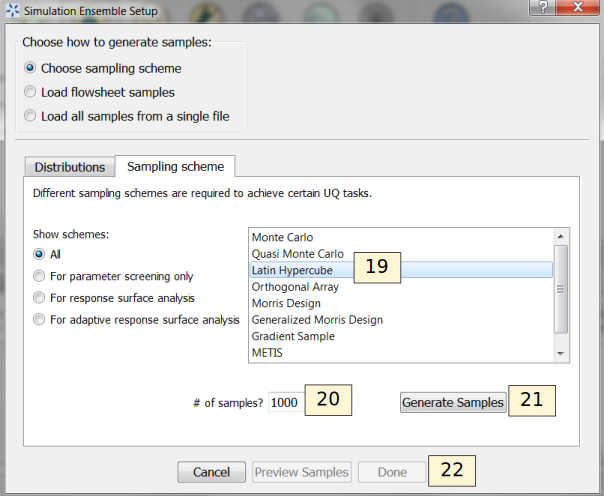
\includegraphics[scale=0.55]{Chapt_surrogates/figs/uqSample2}
		\caption{Sample Methods}
		\label{fig.tut.sur.new.uq.sample2}
	\end{center}
\end{figure}
\begin{enumerate}
\setcounter{enumi}{22}
\item Once the samples have been generated a new sample ensemble displays in the UQ tool window (Figure \ref{fig.tut.sur.new.uq.sample3}).  Click \textbf{\underline{Launch}} to run and generate the samples.
\end{enumerate}
\begin{figure}[H]
	\begin{center}
		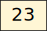
\includegraphics[scale=0.55]{Chapt_surrogates/figs/uqSample3}
		\caption{Run Samples}
		\label{fig.tut.sur.new.uq.sample3}
	\end{center}
\end{figure}

\subsection{Data Selection}

Initial and validation data can be specified by creating filters that specify subsets of flowsheet data. In this tutorial only initial data will be used. A filter must be created to separate the results of the single test run from the UQ samples.

\begin{enumerate}
	\setcounter{enumi}{23}
	\item Click on the \textbf{\underline{Surrogates}} button from the Home window. The surrogate tool displays \ref{fig.tut.sur.data}.
	\item Select ``ALAMO'' from the \textbf{\underline{Tool}} drop-down list.
	\item Click \textbf{\underline{Edit Filters}} in the \textbf{\underline{Flowsheet Results}} section to create a filter.
\end{enumerate} 
\begin{figure}[H]
	\begin{center}
		
\includegraphics[scale=0.55]{Chapt_surrogates/figs/data}
		\caption{Surrogate Data}
		\label{fig.tut.sur.data}
	\end{center}
\end{figure}

\begin{enumerate}
	\setcounter{enumi}{26}
	\item Figure \ref{fig.tut.sur.dataFilter} displays the Data Filter Editor. 
	\item Add the filter for initial data.
	\begin{enumerate}
		\item Click \bu{New Filter}, and enter ``Initial'' as the filter name.
		\item Click \bu{Add Rule}.
		\item In the ``Term 1'' column enter: set (no quotes).
		\item In the ``Term 2'' column enter: ``UQ\_Ensemble'' (with quotes).
		\item In the ``Operator'' column select ``=.''	
	\end{enumerate}
	\item Click \textbf{\underline{Done}}.
\end{enumerate}
\begin{figure}[H]
	\begin{center}
		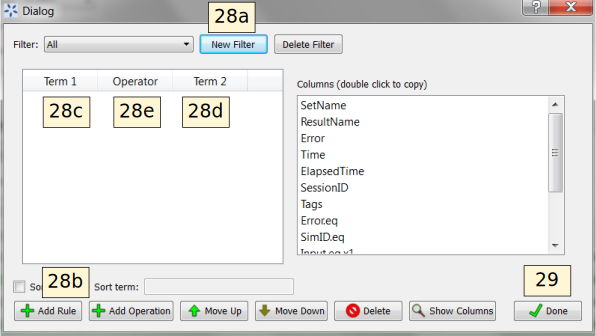
\includegraphics[scale=0.55]{Chapt_surrogates/figs/dataFilter}
		\caption{Data Filter Dialog}
		\label{fig.tut.sur.dataFilter}
	\end{center}
\end{figure}

\subsection{Variable Selection}
In this section, input and output variables need to be selected. Generally, any input variables that vary in the data set should be selected. However, in some cases, variables may be found to have no, or very little, effect on the outputs. Only the output variables of interest need to be selected. Note: Each output is independent from each other and for the model building, selecting one output is the same as selecting more.

\begin{enumerate}
	\setcounter{enumi}{29}
	\item Select the \textbf{\underline{Variable}s} tab (Figure \ref{fig.tut.sur.vaiables}).
	\item Select the checkbox for both input variables.
	\item Select the checkbox for both output variables.
\end{enumerate}
\begin{figure}[H]
	\begin{center}
		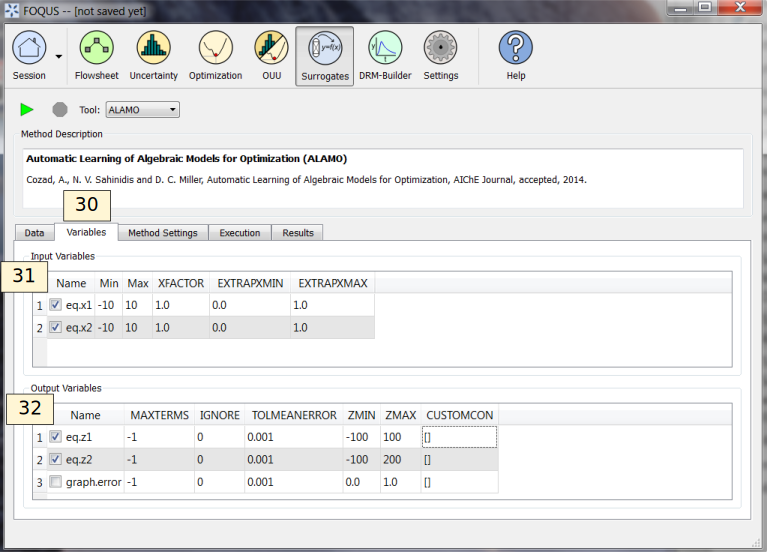
\includegraphics[scale=0.55]{Chapt_surrogates/figs/variables}
		\caption{Variable Selection}
		\label{fig.tut.sur.vaiables}
	\end{center}
\end{figure}

\subsection{Method Settings}
\label{tutorial.alamo.methodsettings}
The most important feature to generate "good" algebraic models is to configure the settings accordingly to the problem to be solved.  Each setting has a good description in FOQUS. The JSON parser is used to read method settings values. Strings must be contained in quotes. Lists have the following format: [element 1, element 2].

\begin{enumerate}
	\setcounter{enumi}{32}
	\item Click on the \textbf{\underline{Method Settings}} tab (see Figure \ref{fig.alamo.method.settigs}).
	\item Set the \textbf{\underline{FOQUS Model (for UQ)}} to ``ALAMO\_tutorial\_UQ.py.'' 
	\item Set the \textbf{\underline{FOQUS Model (for Flowsheet)}} to ``ALAMO\_tutorial\_FS.py''
	\item Set \textbf{\underline{Initial Data Filter}} to ``Initial.''
	\item Set \textbf{\underline{SAMPLER}} to select the adaptive sampling method: ``None'' ``Random'' or ``SNOBFIT.'' Use ``None'' in this tutorial.
	\item Set \textbf{\underline{MONOMIALPOWER}} to select the single variable term powers to [1,2,3].
	\item Set \textbf{\underline{MULTI2POWER}} to select the two variable term powers to [1].
	\item Select functions to be considered as basis functions (\textbf{\underline{EXPFCNS}}, \textbf{\underline{LOGFCNS}}, \textbf{\underline{SINFCNS}}, \textbf{\underline{COSFCNS}}).
	\item Leave the rest of settings as default (see Table \ref{tutorial.alamo.table}).
	\item Save this FOQUS session for use in the ACOSSO and BSS-ANOVA tutorials.
\end{enumerate}
\begin{figure}[H]
	\begin{center}
		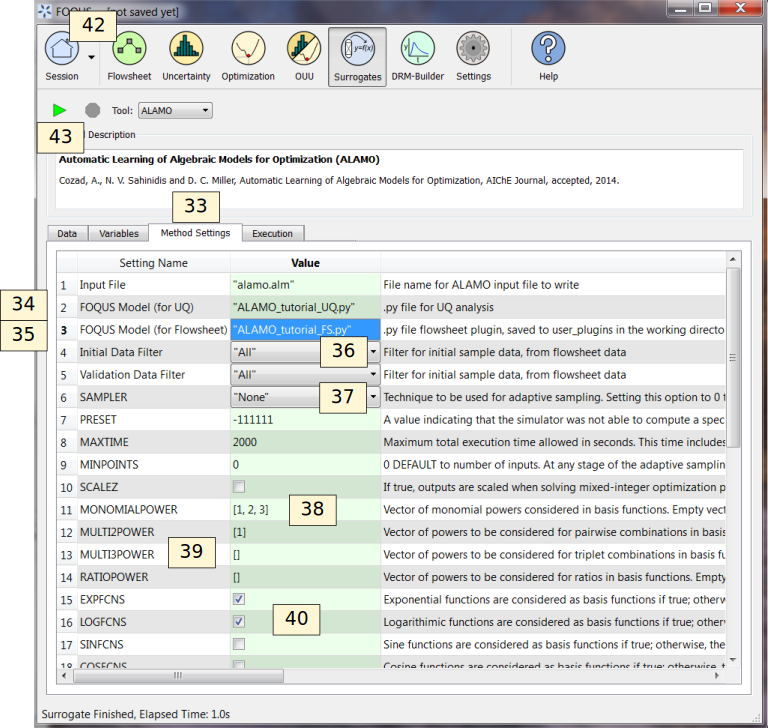
\includegraphics[scale=0.55]{Chapt_surrogates/figs/alamo_settings}
		\caption{ALAMO Method Settings}
		\label{fig.alamo.method.settigs}
	\end{center}
\end{figure}

\subsection{Execution}

\begin{enumerate}
	\setcounter{enumi}{42}
	\item Click the \bu{Run} icon at the top of the window.
	\item The ALAMO \bu{Execution} tab starts displaying execution file path, sub-directories, input files, and output files.
\begin{enumerate}
	\item ALAMO version.
	\item License Information.
	\item Step 0 displays the data set to be used by ALAMO.
	\item Step 1 displays the modeler used by ALAMO to generate the algebraic model.
	\item Once the surrogate model has finished, the equations are displayed in the execution window. It may be necessary to scroll up a little. The result is shown in Figure \ref{fig.alamo.res}.
	\item Finally, the statistics display the quality metrics of the models generated.
\end{enumerate}
\end{enumerate}

\begin{figure}[H]
	\begin{center}
		\includegraphics[scale=0.4]{Chapt_surrogates/figs/alamo_exec}
		\caption{ALAMO Execution}
		\label{fig.alamo.res}
	\end{center}
\end{figure}

\subsection{Results}
	The results are exported as a PSUADE driver file that can be used perform UQ analysis of the models, and a FOQUS Python plugin model that allows it to be used in a FOQUS flowsheet. The equations can also be viewed in the results section.
	
	See tutorial Section \ref{tutorial.surrogate.uq} and \ref{tutorial.surrogate.fs} for information about analyzing the model with the UQ tools or running the model on the flowsheet.
	
	As mentioned in section \ref{tutorial.alamo.methodsettings} the method settings are very important. A brief description and hints are included in Table \ref{tutorial.alamo.table}.

\begin{center}

\begin{longtable}{|p{.30\textwidth}|p{.70\textwidth} |}
\caption{ALAMO Method Settings}
\label{tutorial.alamo.table} \\

		\hline
			\textbf{Method Settings} & \textbf{Description} \\		\hline
			Initial Data Filter & Filter to be applied to the initial data set. Data filters help the user to generate models based on specific data for each variable.  \\	\hline
			Validation Data filter & Data set used to compute model errors at the validation phase. The number of data points in a preexisting validation data set can be specified by the user.\\	\hline
			SAMPLER & Adaptative sampling method to be used. Options: "None", "Random" and "SNOBFIT". Adaptive sampling method to be used by ALAMO when more sampling points are needed by the model. If \bu{Random} is used a simulator must be provided by the user. If \bu{SNOBFIT} is used a simulator must be provided by the user and MATLAB must be installed.\\	\hline
			MAXTIME& Maximum execution time in seconds. This time includes all the steps on the algorithm, if simulations are needed they run in this time.\\	\hline
			MINPOINTS& Convergence is assessed only if the simulator is able to compute the output variables for at least MINPOINTS of the data set. A reduced number of MINPOINTS may reduce the computational time to get a model, but also reduces the accuracy of the model. MINPOINTS must be a positive integer. \\ \hline
			PRESET&Value to be used if the simulator fails. This value must be carefully chosen to be an otherwise not realizable value for the output variables.\\ \hline
			MONOMIALPOWERS &  Vector of monomial powers to be considered as basis functions, use empty vector for none []. Exponential terms allowed in the algebraic model.  i.e., if selecting [1,2] the model considers x1 and x1**2 as basis functions. \\ \hline
			MULTI2POWER & Vector of pairwise combination of powers to be considered as basis functions. Pairwise combination of powers allowed in the algebraic model. i.e., [1,2] allows terms like x1*x2 in the algebraic model.\\ \hline
			MULTI3POWER & Vector of three variables combinations of powers to be considered as basis functions. \\ \hline
			\raggedright{EXPFCNS, LOGFCNS, SINFCNS, COSFCNS functions}& Use or not of exp, log, sin, and cos functions as basis functions in the model. \\ \hline
			RATIOPOWER& Vector of ratio combinations of powers to be considered in the basis functions. Ratio combinations of powers are [empty as default].\\ \hline
			Radial Basis Functions& Radial basis functions centered around the data set provided by the user. These functions are Gaussian and are deactivated if their textual representation requires more than 128 characters (in the case of too many input variables and/or datapoints). \\ \hline
			RBF parameter&Constant penalty used in the Gaussian radial basis functions.  \\ \hline
			Modeler & Fitness metric to be used for model building. Options: BIC (Bayesian Information Criterion), Mallow's Cp, AICc (Corrected Akaike's Information Criterio), HQC (Hannan-Quinn Information Criterion), MSE (Mean Square Error), and Convex Penalty. \\ \hline
			ConvPen& Convex penalty term. Used if Convex Penalty is selected. \\ \hline
			Regularizer & Regularization method is used to reduce the number of potential basis functions before the optimization.\\ \hline 
			Tolrelmetric & Convergence tolerance for the chosen fitness metric is needed to terminate the algorithm. \\ \hline
			ScaleZ&If used, the variables are scaled prior to the optimization problem is solved. The problem is solved using a mathematical programming solver. Usually, scaling the variables may help the optimization procedure.\\ \hline
			GAMS&GAMS is the software used to solve the optimization problems. The executable path is expected or the user must declare GAMS.exe in the environment path.\\ \hline
			GAMS Solver&Solver to be used by GAMS to solve the optimization problems. Mixed integer quadratic programming solver is expected like BARON (other solvers can be used).\\ \hline
			MIPOPTCR & Relative convergence tolerance for the optimization problems solved in GAMS. The optimization problem is solved when the optcr is reached. 5 to 1 \% is expected (0.005 to 0.001).\\ \hline
			MIPOPTCA & Absolute convergence tolerance for mixed-integer optimization problems. This must be a nonnegative scalar. \\ \hline
			Linear error & If true, a linear objective function is used when solving the mixed integer optimization problems; otherwise, a quadratic objective function is used. \\ \hline
			\raggedright{Constraint Regression (CONREG)} & Specify whether constraint regression is used or not, if true bounds on output variables are enforced. \\ \hline
			CRNCUSTOM & If true, Custom constraints are entered in the Variable tab.\\ \hline
			CRNINITIAL& Number of random bounding points at which constraints are sampled initially (must be a nonnegative integer). \\ \hline
			CRNMAXITER & Maximum allowed constrained regressions iterations. Constraints are enforced on additional points during each iteration (must be positive integer). \\ \hline
			CRNVIOL & Number of bounding points added per round per bound in each iteration (must be positive integer). \\ \hline
			CRNTRIALS&Number of random trial bounding points per round of constrained regression (must be a positive integer). \\ \hline
			CUSTOMBAS&A list of user-supplied custom basis functions can be provided by the user. The parser is not case sensitive and allows for any Fortran functional expression in terms of the XLABELS (symbol \^{} may be used to denote power). \\ \hline
			
%		\end{tabularx}
%	\end{center}

\end{longtable}	
\end{center}	

\section{Tutorial -- ACOSSO}
\label{(sec.surrogate.acosso)}

This tutorial covers the ACOSSO surrogate modeling method. The Adaptive
COmponent Selection and Shrinkage Operator (ACOSSO) surface approximation
was developed under the Smoothing Spline Analysis of Variance (SS-ANOVA)
modeling framework \citep{Storlie_2011}. As it is a smoothing type method,
ACOSSO works best when the underlying function is somewhat smooth. For
functions which are known to have sharp changes or peaks, etc., other
methods may be more appropriate. Since it implicitly performs variable
selection, ACOSSO can also work well when there are a large number of input
variables. 
The ACOSSO procedure also allows for
categorical inputs \citep{Storlie_2013}.
 
This tutorial uses the same flowsheet and sample setup as the ALAMO
tutorial in Section \ref{sec.surrogate.alamo}. The statistics software
``R'' is also required to use ACOSSO and BSS-ANOVA. Before starting this
tutorial, you will need to install R version 3.1 or later (see \href{http://cran.r-project.org/}{\textcolor{blue}{https://cran.r-project.org/}}). 

Once R is installed, you will need to install the ``quadprog''
package. ACOSSO requires this package for solving quadratic
programming problems. You will only need to perform this step once. 

\begin{enumerate}
\item{Start R. In Windows, this must be done with administrative
  privileges.  Either run this from an administrator account, or
  right-click ``R x64 3.1.2'' and click ``Run with administrator'' and type
  in administrator credentials.}
\item{Inside the R console, type:
   \begin{itemize} 
   \item \tt install.packages('quadprog')
   \item \tt library(quadprog)
   \item \tt q()
  \end{itemize}
The first line installs the package. If prompted for a CRAN mirror, select
the one closest to you geographically. The second line loads the
package. The last line quits R. If prompted to save workspace image, choose
`y'.}
\end{enumerate}

Once you have done these steps, ACOSSO is ready to be invoked inside FOQUS.

\begin{enumerate}
	\item{Set the path to the RScript executable.}
		\begin{enumerate}
			\item Click the \bu{Settings} button in the Home window.
			\item Change the RScript path if necessary. The \bu{Browse} button
           opens a file browser that can be used to set the path.
		\end{enumerate}
	\item Complete the ALAMO tutorial in Section \ref{sec.surrogate.alamo} through Step 32, or load the FOQUS session saved after completing the ALAMO tutorial.
	\item Click the \bu{Surrogates} button in the Home window (Figure \ref{fig.acosso.settings}).
	\item Select ``ACOSSO'' in the \bu{Tool} drop-down list.
	\item Select the \bu{Method Settings} tab.
	\item Set ``Data Filter'' to ``Initial.''
	\item Set ``Use Flowsheet Data'' to ``Yes.''
	\item Set ``FOQUS Model (for UQ)'' to ``ACOSSO\_Tutorial\_UQ.py.''
	\item Set ``FOQUS Model (for Flowsheet)'' to ``ACOSSO\_Tutorial\_FS.py.''
	\item Click the \bu{Run} icon (Figure \ref{fig.acosso.settings}).
\end{enumerate}

\begin{figure}[H]
	\begin{center}
		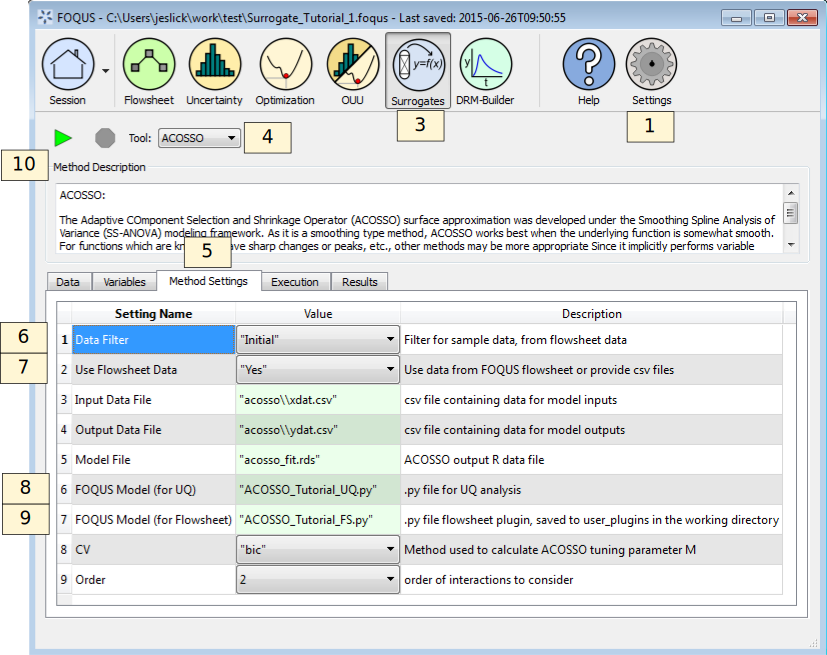
\includegraphics[scale=0.55]{Chapt_surrogates/figs/acosso_settings}
		\caption{ACOSSO Session Set Up}
		\label{fig.acosso.settings}
	\end{center}
\end{figure}

\begin{enumerate}
	\setcounter{enumi}{10}
	\item The execution window will automatically display. While ACOSSO is
     running, the execution window may show warnings, but this is normal.
	\item When the run completes, a UQ driver file is created, allowing the
     ACOSSO surrogate to be used as a user-defined response surface in UQ
     analyses. (See Section \ref{tutorial.surrogate.uq}.)
	\item ACOSSO also produces a flowsheet plugin; however.
\end{enumerate}



\section{Tutorial -- BSS-ANOVA}
\label{(sec.surrogate.bssanova)}

This tutorial covers the BSS-ANOVA surrogate modeling method.  The Bayesian
Smoothing Spline ANOVA (BSS-ANOVA) is essentially a Bayesian version of
ACOSSO \citep{Reich_2009}.  It is Gaussian Process (GP) model with a
non-conventional covariance function that borrows its form from SS-ANOVA.
It tackles the high dimensionality (of inputs) on two fronts: (1) variable
selection to eliminate uninformative variables from the model and (2)
restricting the level of interactions involved among the variables in the
model. This is done through a fully Bayesian approach which can also allow
for categorical input variables with relative ease. Since it is closely
related to ACOSSO, it generally works well in similar settings as
ACOSSO. The BSS-ANOVA procedure also allows for categorical inputs
\citep{Storlie_2013}. In this current implementation, BSS-ANOVA is more
computationally intensive than ACOSSO, so ACOSSO is preferred for faster
surrogate generation. 

This tutorial uses the same flowsheet and sample setup as the ALAMO
tutorial in Section \ref{sec.surrogate.alamo}. The statistics software
``R'' is also required to use ACOSSO and BSS-ANOVA. Before starting this
tutorial, you will need to install R version 3.1 or later (see \href{https://cran.r-project.org/}{\textcolor{blue}{http://cran.r-project.org/}}).

\begin{enumerate}
	\item{Set the path to the RScript executable.}
		\begin{enumerate}
			\item Click the \bu{Settings} button from the Home window.
			\item Change the RScript path if necessary.  The \bu{Browse} button opens a file browser that can be used to set the path.
		\end{enumerate}
	\item Complete the ALAMO tutorial in Section \ref{sec.surrogate.alamo} through Step 32, or load the FOQUS session saved after completing the ALAMO tutorial.
	\item Click the \bu{Surrogates} button from the Home window (Figure \ref{fig.bssanova.settings}).
	\item Select ``BSS-ANOVA'' in the \bu{Tool} drop-down list.
	\item Select the \bu{Method Settings} tab.
	\item Set ``Data Filter'' to ``Initial.''
	\item Set ``Use Flowsheet Data'' to ``Yes.''
	\item Set ``FOQUS Model (for UQ)'' to ``bssanova\_tutorial\_uq.py.''
	\item Set ``FOQUS Model (for Flowsheet)'' to ``bssanova\_tutorial\_fs.py.''
	\item Click the \bu{Run} icon (Figure \ref{fig.bssanova.settings}).
\end{enumerate}

\begin{figure}[H]
	\begin{center}
		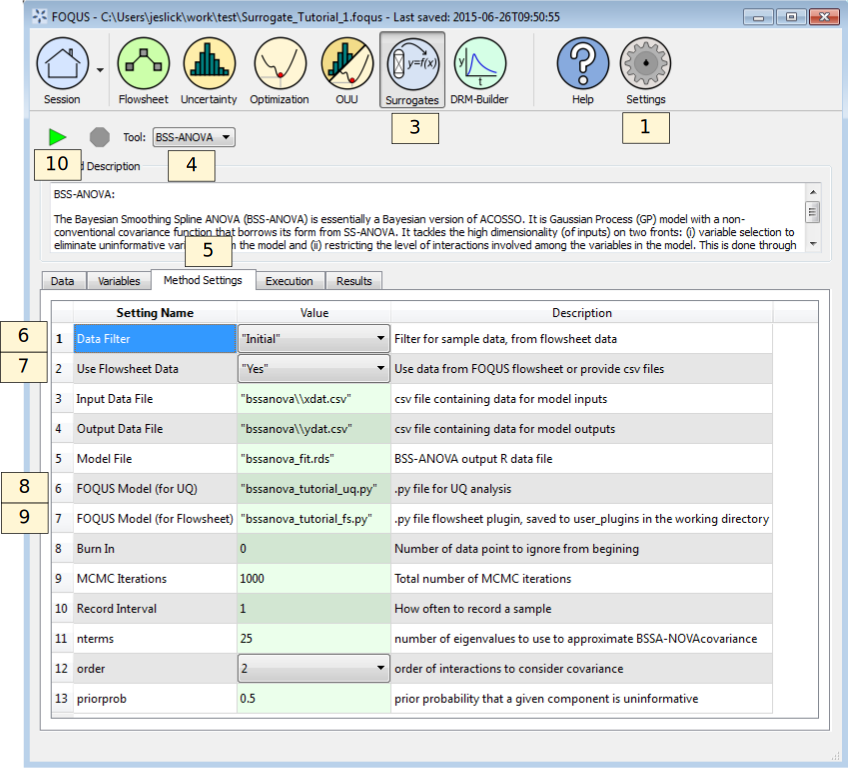
\includegraphics[scale=0.55]{Chapt_surrogates/figs/bssanova_settings}
		\caption{BSS-ANOVA Session Set Up}
		\label{fig.bssanova.settings}
	\end{center}
\end{figure}

\begin{enumerate}
   \setcounter{enumi}{10}
   \item The execution window will automatically display. While BSS-ANOVA is
     running, the execution window may show warnings, but this is normal.
   \item When the run completes, a UQ driver file is created, allowing the
     BSS-ANOVA surrogate to be used as a user-defined response surface in UQ
     analyses. (See Section \ref{tutorial.surrogate.uq}.)
   \item BSS-ANOVA also produces a flowsheet plugin.
\end{enumerate}


\section{Tutorial -- iREVEAL} 
The iREVEAL documentation is currently separate, but will be merged in the next release. The iREVEAL user's manual is included in the FOQUS installation.  There is a link to the manual in the Windows start menu under CCSI Tools\bs FOQUS.

\section{Tutorial -- Surrogates with UQ Tools}
\label{tutorial.surrogate.uq}

For the purpose of this tutorial, we will use ACOSSO to demonstrate the use
of a surrogate within the UQ module. The steps are the same regardless of
the surrogate tool chosen.

To perform the UQ analysis, Python is required for use the ``User Regression'' response surface that will be used.  Before starting this tutorial, you will need to install Python 2.7.x (not Python 3). (See \href{https://www.python.org/downloads/}{\textcolor{blue}{https://www.python.org/downloads/}}). In addition, if *.py files have been re-associated with other executables (e.g. editors), please change the association back to python.exe. 


\begin{enumerate}
\item{Load a fresh session by clicking the \bu{Session} button from the Home window. Select \textbf{\underline{Open Session}} and then navigate to the ``examples/UQ''
  directory. Select ``Rosenbrock\_no\_vectors.foqus.'' This will load a
  session with a simple flowsheet containing a single node.}
\item{Click \bu{Settings} and ensure that (1) FOQUS Flowsheet Run Method is
  set to ``Local'', and that (2) proper paths are set for PSUADE and RScript.} 
\item{Train an ACOSSO surrogate of this node by clicking the
  \bu{Surrogates} button from the Home window.
\begin{enumerate}
\item{Click \bu{Add Samples} and select ``Use Flowsheet''. This will
  display the \bu{Simulation Ensemble Setup} dialog.}
\item{Within this dialog, ensure all variables are set to ``Variable''
  type in the \bu{Distributions} tab. In the \bu{Sampling scheme} tab,
  select ``Monte Carlo'' as your sampling scheme, set the number of
  samples to 100, and then click \bu{Generate Samples} to generate the
  set of input values. Click \bu{Done} to return to the Surrogates screen.}
\item{Once sample generation completes, click the \bu{Uncertainty} button from the Home window.}
\item{Click the \bu{Launch}	button to generate the samples.}
\item{Click the \bu{Surrogates} button from the Home window. The \bu{Data} tab of the Surrogates
  screen should now displays a \bu{Flowsheet Results} table that is populated with
  the values of the new input samples.}
\item{From the \bu{Variables} tab, select all of the checkboxes. (There should
  be six checkboxes for input variables and one checkbox for output variable.) 
  Here, you are defining the inputs and outputs for your surrogate function.}
\item{From the \bu{Method Settings} tab, note the name of the file next to
  ``FOQUS Model (for UQ)''. This will be the name of the UQ driver file
  that contains the Python code that implements the surrogate function.}
\item{On top of this screen, select ``ACOSSO'' as your surrogate tool from the \textbf{\underline{Tool}} drop-down list and then click on the green arrow to start training the surrogate.}
\item{Once complete, a popup window will display, reminding you of the
  location of the drive file. Note the location as you will need this
  information later inside the UQ module.} 
\end{enumerate}
}
\item{Perform a response-surface-based uncertainty analysis by clicking the 
  \bu{Uncertainty} button from the Home window.
\begin{enumerate}
\item{In the \bu{Uncertainty Quantification Simulation Ensembles} table. A row corresponding to the ensemble that was just
  generated for surrogate training should be displayed. This same ensemble can be used or
  a new one can be created to be used as the test data set for analysis. 
  In the row corresponding to the ensemble
  to be analyzed, click the \bu{Analyze} button to proceed. This
  action will bring up an analysis dialog.} 
\item{Within this analysis dialog, navigate to ``Analysis'' section. For
  Step 1, select ``Response Surface''. For Step 3, select ``User
  Regression'' in the first drop-down list. Lastly, for ``User Regression File'',
  browse to the same location as the UQ driver file that was
  generated within the Surrogates module. (This is the same location that
  was previously noted from the popup message.) 
  At this point, your surrogate function is now set up as a user-defined
  response surface and all response-surface-based UQ analyses are accessible.}
\item{Click \bu{Validate} (Step 4) to perform response surface validation. Once
  complete, a figure with cross-validation results will be displayed: 
  a histogram of errors to the left and a plot of predicted values versus
  actual values to the right. For more information, refer to the UQ
  Tutorial in Section \ref{tutorial.uq.rs}.}
\item{Once a ``Response Surface'' has been validated, other UQ analysis options
  are available. Choose ``Uncertainty Analysis'' in Step 5 and click
  \bu{Analyze} to perform uncertainty analysis using your ACOSSO surrogate.}
\end{enumerate}
}
\end{enumerate}

During validation, if the error, ``RSAnalyzer: RSTest\_hs.m does
not exist.'' displays, this is likely caused by incompatibility with the surrogate
and the test data. An example scenario might be your test data has six
inputs, but your surrogate assumes five inputs. This is easily fixed by
returning to the Surrogates screen, clicking on the \bu{Variables}
tab, and making sure the appropriate selections are made (i.e., check off six
inputs instead of just five).

\section{Tutorial -- Surrogates with the Flowsheet}\label{tutorial.surrogate.fs}

This section provides a brief tutorial for using the flowsheet plugin models generated by surrogate modeling methods. In the next FOQUS release all surrogate modeling methods will produce a model that can be run in a FOQUS flowsheet. \textbf{Currently iREVEAL does not produce a flowsheet model.}

\textbf{Before doing this tutorial complete the ALAMO tutorial in Section \ref{sec.surrogate.alamo}.}

\begin{enumerate}
	\item Open FOQUS.  If FOQUS has not been closed since completing the ALAMO tutorial, close it and reopen it. There is a known issue where existing flowsheet model plugins may not update until FOQUS is restarted.
	\item Enter ``FS\_Plugin\_Tutorial'' as the Session Name.
	\item Click the \bu{Flowsheet} button from the Home window.
	\item Click the \bu{Add Node} icon in the left toolbar (see Figure \ref{fig.pg.tut1}).
	\item Click a location for the node in the Flowsheet area.
	\item Enter ``model'' for the node name (without quotes).
	\item Click the \bu{Node Editor} icon in the left toolbar (see Figure \ref{fig.pg.tut1}).
	\item In the \textbf{\underline{Node Editor}}, select ``Plugin'' from the Model \textbf{\underline{Type}} drop-down list. 
	\item Select ``ALAMO\_Tutorial\_FS'' from the \textbf{\underline{Model}} drop-down list. 
	\item Set the \textbf{\underline{Value}} of the \textbf{\underline{Input Variables}} ``eq.x1'' to 2.
	\item Set the \textbf{\underline{Value}} of the \textbf{\underline{Input Variables}} ``eq.x2'' to 3.
	\item Click the \bu{Run} icon in the left toolbar (see Figure \ref{fig.pg.tut1}).
	\item Wait for the Flowsheet evaluation to complete. It should finish successfully.
	\item Check the value of the \textbf{\underline{Output Variables}}; the approximate values should be z1 = 5 and z2 = 13.
\end{enumerate}

\begin{figure}[H]
	\begin{center}
		\includegraphics[scale=0.55]{Chapt_surrogates/figs/fs_plugin}
		\caption{Plugin Flowsheet}
		\label{fig.pg.tut1}
	\end{center}
\end{figure}




	

\chapter{Surrogate Models}\label{chpt.surrogates}

\section{D-RM (Dynamic Reduced Models) Builder}\label{sec.overview.drm}

The Dynamic Reduced Model (D-RM) Builder is a software tool used to generate data-driven dynamic reduced models from high-fidelity dynamic models consisting of differential and algebraic equations (DAEs).  DAE-based models are usually computationally intensive to solve, especially when stiff DAEs are involved.  For instance, the sorbent-based bubbling fluidized bed CO$_2$ adsorber-reactor model contains over 20,000 DAEs and very small time steps ($<$0.001 second) have to be used to solve the stiff equations in the rigorous model.  The D-RMs generated by the D-RM Builder enable much faster computation of the system responses (up to several orders of magnitude faster), which enable the development of an advanced process control framework and the integration of the dynamic models within a large-scale dynamic simulation.

\subsection{Motivating Example}

The solid-sorbent-based bubbling fluidized bed CO$_2$ adsorber-reactor for the post-combustion carbon capture is a good example to which the D-RM Builder tool can be applied.  The dynamics of the adsorber-reactor was modeled by a CCSI team using Aspen Custom Modeler (ACM).  The high-fidelity dynamic model of the twin-bed adsorber-reactor contains over 20,000 equations.  The feed streams include CO$_2$-containing flue gas, solid sorbent, and multiple cooling water streams.  Since some equations are very stiff, a minimum integration time step of 0.001 second has to be used.  As a result, the computer CPU time required to calculate the response of the system over a period of operating time is much longer than the real operating time, especially when there is a change in model inputs (step or ramp change).  The data-driven D-RM can be generated by fitting the system outputs in response to the changes of system inputs through certain plant identification models.  The response of the system to the input changes can be simulated by the ACM model.  The D-RM Builder is provided for a user to configure the input and output variables of interest, prepare a sequence of step changes of input variables, launch ACM simulations, generate a D-RM, and export the D-RM in a form of a MATLAB function file (.m file), which can be called by MATLAB to calculate the system response given the model inputs with a CPU execution time a few orders of magnitude shorter than that required by the ACM model.  The speedup in CPU time enables the implementation of advanced process control (APC) systems.

\subsection{Features List}

The D-RM Builder is an application embedded in the graphic user interface (GUI) of FOQUS.  Data-driven D-RMs can be generated by the D-RM Builder based on a set of high-fidelity model outputs in response to a sequence of input changes within a range of operating conditions.  The D-RM Builder can read the input and output variables pre-configured through SinterConfigGUI application, which is also a part of the FOQUS package.  Through the D-RM Builder GUI, a user can select a set of the pre-configured input variables, specify their lower and upper limits, and prepare a sequence of step changes or ramp changes based on the Latin Hypercube Sampling (LHS) method with desired durations of the step changes to excite the system in a range of frequencies.  The simulations of high-fidelity models, currently implemented for ACM only, can be launched directly in the D-RM Builder through ConsoleSinter, which is also a part of the FOQUS package.  The simulation results can be used to generate the D-RMs.  A separate set of step-change sequence can also be generated and its response be simulated by the ACM model and predicted by the D-RM for validation purpose.  The generated D-RMs and the user inputs for case setup and configuration can be saved in a text file in JSON format with extension ``drmb''.  Once a case file is saved, the user can copy the file to a different directory or to a different computer where the D-RM Builder is installed and open the file later to continue the D-RM building process or visualize the properties of the generated D-RMs.  A D-RM Builder project could also be a subproject of a FOQUS project and saved as a part of FOQUS session.  When a saved FOQUS session file is opened, the D-RM Builder subproject is also opened.

Two types of D-RMs are supported in the current version including the Decoupled A-B Net (DABNet) model \cite{Sentoni_1998}, and the Nonlinear Auto-regressive Moving Average (NARMA) model \cite{Narendra_1997}.  Different building options are provided for the user to choose from including input delays, two-pole Laugerre formulation of DABNet model, and optimization of model parameters.  Both D-RM model types require the training of artificial neural networks (ANNs).  Two ANN training methods, back propagation (BP) and interior point optimization (IPOPT), are provided.  The generated D-RM can be validated by performing another set of high-fidelity model simulations with a different input change sequence and comparing the response to that predicted by the generated D-RMs.  The response calculated by the high-fidelity model and that by the D-RM can be displayed through the D-RM Builder$\text{'}$s GUI.  The accuracy of the generated D-RM can be visualized by comparing the D-RM predictions to the corresponding ACM predictions, including the relative errors and the coefficient of determination R$^2$.  For the state-space based DABNet model, Uncertainty Quantification (UQ) analysis can be performed on the validation data using Unscented Kalman Filter (UKF), providing the covariance matrices of state-space and output variables.  The messages of the model building process including command sequence are displayed in the main text window of the D-RM Builder, which can be saved to a log file for future reference.  The internal parameters of the generated D-RM can be exported to a MATLAB script file, which can be run in MATLAB to initialize a D-RM object instantiated from a MATLAB class.  The results of the high-fidelity model simulations and D-RM predictions for both the training and the validation input sequences can also be exported to text files in comma-separated value (CSV) format, which can be opened by Microsoft® Excel®.

Along with the D-RM Builder application, several MATLAB files are also provided as part of the software tool.  These files define the MATLAB classes that can be used to create the D-RM objects in the MATLAB workspace given the D-RM files exported from the D-RM Builder.  The functions in the D-RM objects can be called to perform dynamic simulations.

\section{Tutorial -- ALAMO}
\label{sec.surrogate.alamo}
This tutorial focuses on the use of the ALAMO tool for building algebraic surrogate models. ALAMO builds simplified algebraic models, which are particularly well suited for rigorous equation oriented optimization. To keep the execution of this tutorial fast, a toy problem is used. In this case study the flowsheet calculations and sample generation are done within FOQUS, alternatively, the user can provide a simulation model such as: Excel, Aspen plus, Aspen custom modeler, etc. 

Note: Before starting this tutorial the ALAMO product must be downloaded from the products page on the CCSI website. The path for the ALAMO executable file must be set in FOQUS settings (see Section \ref{section.settings}).

\subsection{Flowsheet Setup}

\begin{enumerate}
	\item Open FOQUS.
	\item Name the session ``Surrogate\_Tutorial\_1'' (Figure \ref{fig.tut.sur.session}).
\end{enumerate}

\begin{figure}[H]
	\begin{center}
		\includegraphics[scale=0.55]{Chapt_surrogates/figs/session1}
		\caption{Session Set Up}
		\label{fig.tut.sur.session}
	\end{center}
\end{figure}

\begin{enumerate}
	\setcounter{enumi}{2}
	\item Navigate to the Flowsheet Editor (Figure \ref{fig.tut.sur.flowsheet}).
	\item Add a Flowsheet Node named ``eq.''
	\item Display the Node Editor by clicking the \textbf{\underline{Node Editor}} toggle button.
\end{enumerate}
\begin{figure}[H]
	\begin{center}
		\includegraphics[scale=0.55]{Chapt_surrogates/figs/flowsheet}
		\caption{Flowsheet Setup}
		\label{fig.tut.sur.flowsheet}
	\end{center}
\end{figure}
The \textbf{\underline{Node Editor}} displays (Figure \ref{fig.tut.sur.nodeEdit.Input}).  The first step to setting up the node for this problem is to add input and output variables to the node.
%Does more detail need added to #9 below since the figure shows x1 and x2 in the Input Variables menu. Does the user need to know to click on Output Variables to open the Output Variables screen, then enter z1 and z2 under the Name column?
\begin{enumerate}
	\setcounter{enumi}{5}
	\item If the input variables table is not displayed as shown in Figure \ref{fig.tut.sur.nodeEdit.Input}, click the \textbf{\underline{Variables}} tab and then click the \textbf{\underline{Input Variables}} toolbox section.
	\item Add the variables ``x1'' and ``x2'' by clicking the \textbf{\underline{Add}} icon (+) above the input table.
	\item Edit the \textbf{\underline{Min/Max}} value for both variables to be ``-10.0'' and ``10.0.''
	\item Add two output variables ``z1'' and ``z2.''
\end{enumerate}
\begin{figure}[H]
	\begin{center}
		\includegraphics[scale=0.55]{Chapt_surrogates/figs/nodeInput}
		\caption{Node Variables}
		\label{fig.tut.sur.nodeEdit.Input}
	\end{center}
\end{figure}
To keep the execution time short, the node will not be assigned to a simulation model and calculations are performed directly in FOQUS.  
\begin{enumerate}
	\setcounter{enumi}{9}
	\item Click on the \textbf{\underline{Node Script}} tab in the Node Editor to enter the test equation (this step replaces the use of a simulator).
	\item Enter the following equations (Figure \ref{fig.tut.sur.nodeEdit.eq}):
	\begin{verbatim}
		f["z1"] = x["x1"] + x["x2"]
		f["z2"] = x["x1"]**2 + x["x2"]**2
	\end{verbatim}
	The node script calculations are written in Python. The dictionary ``f'' stores output values while the dictionary ``x'' stores input values.

\begin{figure}[H]
	\begin{center}
		\includegraphics[scale=0.55]{Chapt_surrogates/figs/nodeEq}
		\caption{Node Script}
		\label{fig.tut.sur.nodeEdit.eq}
	\end{center}
\end{figure}

	\item Test the model by running the flowsheet with the value ``2'' for ``x1'' and ``x2.'' After running, the output variables should have the values ``4.0'' for ``z1'' and ``8.0'' for ``z2.''
\end{enumerate}


\subsection{Creating Initial Samples}

There are two ways to start an ALAMO run: (1) generate a set of initial data, (2) use ALAMO's adaptive sampling with no initial data and let ALAMO generates its own samples. Adaptive sampling can be used with initial data to generate more points if needed. In this case, initial data is provided and adaptive sampling is used.

\begin{enumerate}
	\setcounter{enumi}{12}
	\item Select the UQ tool by clicking on the \textbf{\underline{Uncertainty}} button on the Home window (Figure \ref{fig.tut.sur.new.uq.ens}).
	\item Click the \textbf{\underline{Add New}} button.
	\item The \textbf{\underline{Add New Ensemble - Model Selection}} dialog will appear. Click \textbf{\underline{OK}} to set up the sampling scheme.
\end{enumerate}
\begin{figure}[H]
	\begin{center}
		\includegraphics[scale=0.55]{Chapt_surrogates/figs/uqNewEns}
		\caption{Add a New Sample Ensemble}
		\label{fig.tut.sur.new.uq.ens}
	\end{center}
\end{figure}
\begin{enumerate}
	\setcounter{enumi}{15}
	\item The sample ensemble setup dialog displays (Figure \ref{fig.tut.sur.new.uq.sample1}).  Select \textbf{\underline{Choose sampling scheme}}. 
	\item Click the \textbf{\underline{All Variable}} button.
	\item Select the \textbf{\underline{Sampling scheme}} tab.
\end{enumerate}
\begin{figure}[H]
	\begin{center}
		\includegraphics[scale=0.55]{Chapt_surrogates/figs/uqSample1}
		\caption{Sample Distributions}
		\label{fig.tut.sur.new.uq.sample1}
	\end{center}
\end{figure}
\begin{enumerate}
	\setcounter{enumi}{18}
	\item The \textbf{\underline{Sampling schem}e} dialog should display (Figure \ref{fig.tut.sur.new.uq.sample2}). Select ``Latin Hypercube'' from the list.
	\item Set the \textbf{\underline{\# of samples}} to ``10.''
	\item Click \textbf{\underline{Generate Samples}}.
	\item Click \textbf{\underline{Done}}.
\end{enumerate}
\begin{figure}[H]
	\begin{center}
		\includegraphics[scale=0.55]{Chapt_surrogates/figs/uqSample2}
		\caption{Sample Methods}
		\label{fig.tut.sur.new.uq.sample2}
	\end{center}
\end{figure}
\begin{enumerate}
\setcounter{enumi}{22}
\item Once the samples have been generated a new sample ensemble displays in the UQ tool window (Figure \ref{fig.tut.sur.new.uq.sample3}).  Click \textbf{\underline{Launch}} to run and generate the samples.
\end{enumerate}
\begin{figure}[H]
	\begin{center}
		\includegraphics[scale=0.55]{Chapt_surrogates/figs/uqSample3}
		\caption{Run Samples}
		\label{fig.tut.sur.new.uq.sample3}
	\end{center}
\end{figure}

\subsection{Data Selection}

Initial and validation data can be specified by creating filters that specify subsets of flowsheet data. In this tutorial only initial data will be used. A filter must be created to separate the results of the single test run from the UQ samples.

\begin{enumerate}
	\setcounter{enumi}{23}
	\item Click on the \textbf{\underline{Surrogates}} button from the Home window. The surrogate tool displays \ref{fig.tut.sur.data}.
	\item Select ``ALAMO'' from the \textbf{\underline{Tool}} drop-down list.
	\item Click \textbf{\underline{Edit Filters}} in the \textbf{\underline{Flowsheet Results}} section to create a filter.
\end{enumerate} 
\begin{figure}[H]
	\begin{center}
		\includegraphics[scale=0.55]{Chapt_surrogates/figs/data}
		\caption{Surrogate Data}
		\label{fig.tut.sur.data}
	\end{center}
\end{figure}

\begin{enumerate}
	\setcounter{enumi}{26}
	\item Figure \ref{fig.tut.sur.dataFilter} displays the Data Filter Editor. 
	\item Add the filter for initial data.
	\begin{enumerate}
		\item Click \bu{New Filter}, and enter ``Initial'' as the filter name.
		\item Click \bu{Add Rule}.
		\item In the ``Term 1'' column enter: set (no quotes).
		\item In the ``Term 2'' column enter: ``UQ\_Ensemble'' (with quotes).
		\item In the ``Operator'' column select ``=.''	
	\end{enumerate}
	\item Click \textbf{\underline{Done}}.
\end{enumerate}
\begin{figure}[H]
	\begin{center}
		\includegraphics[scale=0.55]{Chapt_surrogates/figs/dataFilter}
		\caption{Data Filter Dialog}
		\label{fig.tut.sur.dataFilter}
	\end{center}
\end{figure}

\subsection{Variable Selection}
In this section, input and output variables need to be selected. Generally, any input variables that vary in the data set should be selected. However, in some cases, variables may be found to have no, or very little, effect on the outputs. Only the output variables of interest need to be selected. Note: Each output is independent from each other and for the model building, selecting one output is the same as selecting more.

\begin{enumerate}
	\setcounter{enumi}{29}
	\item Select the \textbf{\underline{Variable}s} tab (Figure \ref{fig.tut.sur.vaiables}).
	\item Select the checkbox for both input variables.
	\item Select the checkbox for both output variables.
\end{enumerate}
\begin{figure}[H]
	\begin{center}
		\includegraphics[scale=0.55]{Chapt_surrogates/figs/variables}
		\caption{Variable Selection}
		\label{fig.tut.sur.vaiables}
	\end{center}
\end{figure}

\subsection{Method Settings}
\label{tutorial.alamo.methodsettings}
The most important feature to generate "good" algebraic models is to configure the settings accordingly to the problem to be solved.  Each setting has a good description in FOQUS. The JSON parser is used to read method settings values. Strings must be contained in quotes. Lists have the following format: [element 1, element 2].

\begin{enumerate}
	\setcounter{enumi}{32}
	\item Click on the \textbf{\underline{Method Settings}} tab (see Figure \ref{fig.alamo.method.settigs}).
	\item Set the \textbf{\underline{FOQUS Model (for UQ)}} to ``ALAMO\_tutorial\_UQ.py.'' 
	\item Set the \textbf{\underline{FOQUS Model (for Flowsheet)}} to ``ALAMO\_tutorial\_FS.py''
	\item Set \textbf{\underline{Initial Data Filter}} to ``Initial.''
	\item Set \textbf{\underline{SAMPLER}} to select the adaptive sampling method: ``None'' ``Random'' or ``SNOBFIT.'' Use ``None'' in this tutorial.
	\item Set \textbf{\underline{MONOMIALPOWER}} to select the single variable term powers to [1,2,3].
	\item Set \textbf{\underline{MULTI2POWER}} to select the two variable term powers to [1].
	\item Select functions to be considered as basis functions (\textbf{\underline{EXPFCNS}}, \textbf{\underline{LOGFCNS}}, \textbf{\underline{SINFCNS}}, \textbf{\underline{COSFCNS}}).
	\item Leave the rest of settings as default (see Table \ref{tutorial.alamo.table}).
	\item Save this FOQUS session for use in the ACOSSO and BSS-ANOVA tutorials.
\end{enumerate}
\begin{figure}[H]
	\begin{center}
		\includegraphics[scale=0.55]{Chapt_surrogates/figs/alamo_settings}
		\caption{ALAMO Method Settings}
		\label{fig.alamo.method.settigs}
	\end{center}
\end{figure}

\subsection{Execution}

\begin{enumerate}
	\setcounter{enumi}{42}
	\item Click the \bu{Run} icon at the top of the window.
	\item The ALAMO \bu{Execution} tab starts displaying execution file path, sub-directories, input files, and output files.
\begin{enumerate}
	\item ALAMO version.
	\item License Information.
	\item Step 0 displays the data set to be used by ALAMO.
	\item Step 1 displays the modeler used by ALAMO to generate the algebraic model.
	\item Once the surrogate model has finished, the equations are displayed in the execution window. It may be necessary to scroll up a little. The result is shown in Figure \ref{fig.alamo.res}.
	\item Finally, the statistics display the quality metrics of the models generated.
\end{enumerate}
\end{enumerate}

\begin{figure}[H]
	\begin{center}
		\includegraphics[scale=0.4]{Chapt_surrogates/figs/alamo_exec}
		\caption{ALAMO Execution}
		\label{fig.alamo.res}
	\end{center}
\end{figure}

\subsection{Results}
	The results are exported as a PSUADE driver file that can be used perform UQ analysis of the models, and a FOQUS Python plugin model that allows it to be used in a FOQUS flowsheet. The equations can also be viewed in the results section.
	
	See tutorial Section \ref{tutorial.surrogate.uq} and \ref{tutorial.surrogate.fs} for information about analyzing the model with the UQ tools or running the model on the flowsheet.
	
	As mentioned in section \ref{tutorial.alamo.methodsettings} the method settings are very important. A brief description and hints are included in Table \ref{tutorial.alamo.table}.

\begin{center}

\begin{longtable}{|p{.30\textwidth}|p{.70\textwidth} |}
\caption{ALAMO Method Settings}
\label{tutorial.alamo.table} \\

		\hline
			\textbf{Method Settings} & \textbf{Description} \\		\hline
			Initial Data Filter & Filter to be applied to the initial data set. Data filters help the user to generate models based on specific data for each variable.  \\	\hline
			Validation Data filter & Data set used to compute model errors at the validation phase. The number of data points in a preexisting validation data set can be specified by the user.\\	\hline
			SAMPLER & Adaptative sampling method to be used. Options: "None", "Random" and "SNOBFIT". Adaptive sampling method to be used by ALAMO when more sampling points are needed by the model. If \bu{Random} is used a simulator must be provided by the user. If \bu{SNOBFIT} is used a simulator must be provided by the user and MATLAB must be installed.\\	\hline
			MAXTIME& Maximum execution time in seconds. This time includes all the steps on the algorithm, if simulations are needed they run in this time.\\	\hline
			MINPOINTS& Convergence is assessed only if the simulator is able to compute the output variables for at least MINPOINTS of the data set. A reduced number of MINPOINTS may reduce the computational time to get a model, but also reduces the accuracy of the model. MINPOINTS must be a positive integer. \\ \hline
			PRESET&Value to be used if the simulator fails. This value must be carefully chosen to be an otherwise not realizable value for the output variables.\\ \hline
			MONOMIALPOWERS &  Vector of monomial powers to be considered as basis functions, use empty vector for none []. Exponential terms allowed in the algebraic model.  i.e., if selecting [1,2] the model considers x1 and x1**2 as basis functions. \\ \hline
			MULTI2POWER & Vector of pairwise combination of powers to be considered as basis functions. Pairwise combination of powers allowed in the algebraic model. i.e., [1,2] allows terms like x1*x2 in the algebraic model.\\ \hline
			MULTI3POWER & Vector of three variables combinations of powers to be considered as basis functions. \\ \hline
			\raggedright{EXPFCNS, LOGFCNS, SINFCNS, COSFCNS functions}& Use or not of exp, log, sin, and cos functions as basis functions in the model. \\ \hline
			RATIOPOWER& Vector of ratio combinations of powers to be considered in the basis functions. Ratio combinations of powers are [empty as default].\\ \hline
			Radial Basis Functions& Radial basis functions centered around the data set provided by the user. These functions are Gaussian and are deactivated if their textual representation requires more than 128 characters (in the case of too many input variables and/or datapoints). \\ \hline
			RBF parameter&Constant penalty used in the Gaussian radial basis functions.  \\ \hline
			Modeler & Fitness metric to be used for model building. Options: BIC (Bayesian Information Criterion), Mallow's Cp, AICc (Corrected Akaike's Information Criterio), HQC (Hannan-Quinn Information Criterion), MSE (Mean Square Error), and Convex Penalty. \\ \hline
			ConvPen& Convex penalty term. Used if Convex Penalty is selected. \\ \hline
			Regularizer & Regularization method is used to reduce the number of potential basis functions before the optimization.\\ \hline 
			Tolrelmetric & Convergence tolerance for the chosen fitness metric is needed to terminate the algorithm. \\ \hline
			ScaleZ&If used, the variables are scaled prior to the optimization problem is solved. The problem is solved using a mathematical programming solver. Usually, scaling the variables may help the optimization procedure.\\ \hline
			GAMS&GAMS is the software used to solve the optimization problems. The executable path is expected or the user must declare GAMS.exe in the environment path.\\ \hline
			GAMS Solver&Solver to be used by GAMS to solve the optimization problems. Mixed integer quadratic programming solver is expected like BARON (other solvers can be used).\\ \hline
			MIPOPTCR & Relative convergence tolerance for the optimization problems solved in GAMS. The optimization problem is solved when the optcr is reached. 5 to 1 \% is expected (0.005 to 0.001).\\ \hline
			MIPOPTCA & Absolute convergence tolerance for mixed-integer optimization problems. This must be a nonnegative scalar. \\ \hline
			Linear error & If true, a linear objective function is used when solving the mixed integer optimization problems; otherwise, a quadratic objective function is used. \\ \hline
			\raggedright{Constraint Regression (CONREG)} & Specify whether constraint regression is used or not, if true bounds on output variables are enforced. \\ \hline
			CRNCUSTOM & If true, Custom constraints are entered in the Variable tab.\\ \hline
			CRNINITIAL& Number of random bounding points at which constraints are sampled initially (must be a nonnegative integer). \\ \hline
			CRNMAXITER & Maximum allowed constrained regressions iterations. Constraints are enforced on additional points during each iteration (must be positive integer). \\ \hline
			CRNVIOL & Number of bounding points added per round per bound in each iteration (must be positive integer). \\ \hline
			CRNTRIALS&Number of random trial bounding points per round of constrained regression (must be a positive integer). \\ \hline
			CUSTOMBAS&A list of user-supplied custom basis functions can be provided by the user. The parser is not case sensitive and allows for any Fortran functional expression in terms of the XLABELS (symbol \^{} may be used to denote power). \\ \hline
			
%		\end{tabularx}
%	\end{center}

\end{longtable}	
\end{center}	

\section{Tutorial -- ACOSSO}
\label{(sec.surrogate.acosso)}

This tutorial covers the ACOSSO surrogate modeling method. The Adaptive
COmponent Selection and Shrinkage Operator (ACOSSO) surface approximation
was developed under the Smoothing Spline Analysis of Variance (SS-ANOVA)
modeling framework \citep{Storlie_2011}. As it is a smoothing type method,
ACOSSO works best when the underlying function is somewhat smooth. For
functions which are known to have sharp changes or peaks, etc., other
methods may be more appropriate. Since it implicitly performs variable
selection, ACOSSO can also work well when there are a large number of input
variables. 
The ACOSSO procedure also allows for
categorical inputs \citep{Storlie_2013}.
 
This tutorial uses the same flowsheet and sample setup as the ALAMO
tutorial in Section \ref{sec.surrogate.alamo}. The statistics software
``R'' is also required to use ACOSSO and BSS-ANOVA. Before starting this
tutorial, you will need to install R version 3.1 or later (see \href{http://cran.r-project.org/}{\textcolor{blue}{https://cran.r-project.org/}}). 

Once R is installed, you will need to install the ``quadprog''
package. ACOSSO requires this package for solving quadratic
programming problems. You will only need to perform this step once. 

\begin{enumerate}
\item{Start R. In Windows, this must be done with administrative
  privileges.  Either run this from an administrator account, or
  right-click ``R x64 3.1.2'' and click ``Run with administrator'' and type
  in administrator credentials.}
\item{Inside the R console, type:
   \begin{itemize} 
   \item \tt install.packages('quadprog')
   \item \tt library(quadprog)
   \item \tt q()
  \end{itemize}
The first line installs the package. If prompted for a CRAN mirror, select
the one closest to you geographically. The second line loads the
package. The last line quits R. If prompted to save workspace image, choose
`y'.}
\end{enumerate}

Once you have done these steps, ACOSSO is ready to be invoked inside FOQUS.

\begin{enumerate}
	\item{Set the path to the RScript executable.}
		\begin{enumerate}
			\item Click the \bu{Settings} button in the Home window.
			\item Change the RScript path if necessary. The \bu{Browse} button
           opens a file browser that can be used to set the path.
		\end{enumerate}
	\item Complete the ALAMO tutorial in Section \ref{sec.surrogate.alamo} through Step 32, or load the FOQUS session saved after completing the ALAMO tutorial.
	\item Click the \bu{Surrogates} button in the Home window (Figure \ref{fig.acosso.settings}).
	\item Select ``ACOSSO'' in the \bu{Tool} drop-down list.
	\item Select the \bu{Method Settings} tab.
	\item Set ``Data Filter'' to ``Initial.''
	\item Set ``Use Flowsheet Data'' to ``Yes.''
	\item Set ``FOQUS Model (for UQ)'' to ``ACOSSO\_Tutorial\_UQ.py.''
	\item Set ``FOQUS Model (for Flowsheet)'' to ``ACOSSO\_Tutorial\_FS.py.''
	\item Click the \bu{Run} icon (Figure \ref{fig.acosso.settings}).
\end{enumerate}

\begin{figure}[H]
	\begin{center}
		\includegraphics[scale=0.55]{Chapt_surrogates/figs/acosso_settings}
		\caption{ACOSSO Session Set Up}
		\label{fig.acosso.settings}
	\end{center}
\end{figure}

\begin{enumerate}
	\setcounter{enumi}{10}
	\item The execution window will automatically display. While ACOSSO is
     running, the execution window may show warnings, but this is normal.
	\item When the run completes, a UQ driver file is created, allowing the
     ACOSSO surrogate to be used as a user-defined response surface in UQ
     analyses. (See Section \ref{tutorial.surrogate.uq}.)
	\item ACOSSO also produces a flowsheet plugin; however.
\end{enumerate}



\section{Tutorial -- BSS-ANOVA}
\label{(sec.surrogate.bssanova)}

This tutorial covers the BSS-ANOVA surrogate modeling method.  The Bayesian
Smoothing Spline ANOVA (BSS-ANOVA) is essentially a Bayesian version of
ACOSSO \citep{Reich_2009}.  It is Gaussian Process (GP) model with a
non-conventional covariance function that borrows its form from SS-ANOVA.
It tackles the high dimensionality (of inputs) on two fronts: (1) variable
selection to eliminate uninformative variables from the model and (2)
restricting the level of interactions involved among the variables in the
model. This is done through a fully Bayesian approach which can also allow
for categorical input variables with relative ease. Since it is closely
related to ACOSSO, it generally works well in similar settings as
ACOSSO. The BSS-ANOVA procedure also allows for categorical inputs
\citep{Storlie_2013}. In this current implementation, BSS-ANOVA is more
computationally intensive than ACOSSO, so ACOSSO is preferred for faster
surrogate generation. 

This tutorial uses the same flowsheet and sample setup as the ALAMO
tutorial in Section \ref{sec.surrogate.alamo}. The statistics software
``R'' is also required to use ACOSSO and BSS-ANOVA. Before starting this
tutorial, you will need to install R version 3.1 or later (see \href{https://cran.r-project.org/}{\textcolor{blue}{http://cran.r-project.org/}}).

\begin{enumerate}
	\item{Set the path to the RScript executable.}
		\begin{enumerate}
			\item Click the \bu{Settings} button from the Home window.
			\item Change the RScript path if necessary.  The \bu{Browse} button opens a file browser that can be used to set the path.
		\end{enumerate}
	\item Complete the ALAMO tutorial in Section \ref{sec.surrogate.alamo} through Step 32, or load the FOQUS session saved after completing the ALAMO tutorial.
	\item Click the \bu{Surrogates} button from the Home window (Figure \ref{fig.bssanova.settings}).
	\item Select ``BSS-ANOVA'' in the \bu{Tool} drop-down list.
	\item Select the \bu{Method Settings} tab.
	\item Set ``Data Filter'' to ``Initial.''
	\item Set ``Use Flowsheet Data'' to ``Yes.''
	\item Set ``FOQUS Model (for UQ)'' to ``bssanova\_tutorial\_uq.py.''
	\item Set ``FOQUS Model (for Flowsheet)'' to ``bssanova\_tutorial\_fs.py.''
	\item Click the \bu{Run} icon (Figure \ref{fig.bssanova.settings}).
\end{enumerate}

\begin{figure}[H]
	\begin{center}
		\includegraphics[scale=0.55]{Chapt_surrogates/figs/bssanova_settings}
		\caption{BSS-ANOVA Session Set Up}
		\label{fig.bssanova.settings}
	\end{center}
\end{figure}

\begin{enumerate}
   \setcounter{enumi}{10}
   \item The execution window will automatically display. While BSS-ANOVA is
     running, the execution window may show warnings, but this is normal.
   \item When the run completes, a UQ driver file is created, allowing the
     BSS-ANOVA surrogate to be used as a user-defined response surface in UQ
     analyses. (See Section \ref{tutorial.surrogate.uq}.)
   \item BSS-ANOVA also produces a flowsheet plugin.
\end{enumerate}


\section{Tutorial -- iREVEAL} 
The iREVEAL documentation is currently separate, but will be merged in the next release. The iREVEAL user's manual is included in the FOQUS installation.  There is a link to the manual in the Windows start menu under CCSI Tools\bs FOQUS.

\section{Tutorial -- Surrogates with UQ Tools}
\label{tutorial.surrogate.uq}

For the purpose of this tutorial, we will use ACOSSO to demonstrate the use
of a surrogate within the UQ module. The steps are the same regardless of
the surrogate tool chosen.

To perform the UQ analysis, Python is required for use the ``User Regression'' response surface that will be used.  Before starting this tutorial, you will need to install Python 2.7.x (not Python 3). (See \href{https://www.python.org/downloads/}{\textcolor{blue}{https://www.python.org/downloads/}}). In addition, if *.py files have been re-associated with other executables (e.g. editors), please change the association back to python.exe. 


\begin{enumerate}
\item{Load a fresh session by clicking the \bu{Session} button from the Home window. Select \textbf{\underline{Open Session}} and then navigate to the ``examples/UQ''
  directory. Select ``Rosenbrock\_no\_vectors.foqus.'' This will load a
  session with a simple flowsheet containing a single node.}
\item{Click \bu{Settings} and ensure that (1) FOQUS Flowsheet Run Method is
  set to ``Local'', and that (2) proper paths are set for PSUADE and RScript.} 
\item{Train an ACOSSO surrogate of this node by clicking the
  \bu{Surrogates} button from the Home window.
\begin{enumerate}
\item{Click \bu{Add Samples} and select ``Use Flowsheet''. This will
  display the \bu{Simulation Ensemble Setup} dialog.}
\item{Within this dialog, ensure all variables are set to ``Variable''
  type in the \bu{Distributions} tab. In the \bu{Sampling scheme} tab,
  select ``Monte Carlo'' as your sampling scheme, set the number of
  samples to 100, and then click \bu{Generate Samples} to generate the
  set of input values. Click \bu{Done} to return to the Surrogates screen.}
\item{Once sample generation completes, click the \bu{Uncertainty} button from the Home window.}
\item{Click the \bu{Launch}	button to generate the samples.}
\item{Click the \bu{Surrogates} button from the Home window. The \bu{Data} tab of the Surrogates
  screen should now displays a \bu{Flowsheet Results} table that is populated with
  the values of the new input samples.}
\item{From the \bu{Variables} tab, select all of the checkboxes. (There should
  be six checkboxes for input variables and one checkbox for output variable.) 
  Here, you are defining the inputs and outputs for your surrogate function.}
\item{From the \bu{Method Settings} tab, note the name of the file next to
  ``FOQUS Model (for UQ)''. This will be the name of the UQ driver file
  that contains the Python code that implements the surrogate function.}
\item{On top of this screen, select ``ACOSSO'' as your surrogate tool from the \textbf{\underline{Tool}} drop-down list and then click on the green arrow to start training the surrogate.}
\item{Once complete, a popup window will display, reminding you of the
  location of the drive file. Note the location as you will need this
  information later inside the UQ module.} 
\end{enumerate}
}
\item{Perform a response-surface-based uncertainty analysis by clicking the 
  \bu{Uncertainty} button from the Home window.
\begin{enumerate}
\item{In the \bu{Uncertainty Quantification Simulation Ensembles} table. A row corresponding to the ensemble that was just
  generated for surrogate training should be displayed. This same ensemble can be used or
  a new one can be created to be used as the test data set for analysis. 
  In the row corresponding to the ensemble
  to be analyzed, click the \bu{Analyze} button to proceed. This
  action will bring up an analysis dialog.} 
\item{Within this analysis dialog, navigate to ``Analysis'' section. For
  Step 1, select ``Response Surface''. For Step 3, select ``User
  Regression'' in the first drop-down list. Lastly, for ``User Regression File'',
  browse to the same location as the UQ driver file that was
  generated within the Surrogates module. (This is the same location that
  was previously noted from the popup message.) 
  At this point, your surrogate function is now set up as a user-defined
  response surface and all response-surface-based UQ analyses are accessible.}
\item{Click \bu{Validate} (Step 4) to perform response surface validation. Once
  complete, a figure with cross-validation results will be displayed: 
  a histogram of errors to the left and a plot of predicted values versus
  actual values to the right. For more information, refer to the UQ
  Tutorial in Section \ref{tutorial.uq.rs}.}
\item{Once a ``Response Surface'' has been validated, other UQ analysis options
  are available. Choose ``Uncertainty Analysis'' in Step 5 and click
  \bu{Analyze} to perform uncertainty analysis using your ACOSSO surrogate.}
\end{enumerate}
}
\end{enumerate}

During validation, if the error, ``RSAnalyzer: RSTest\_hs.m does
not exist.'' displays, this is likely caused by incompatibility with the surrogate
and the test data. An example scenario might be your test data has six
inputs, but your surrogate assumes five inputs. This is easily fixed by
returning to the Surrogates screen, clicking on the \bu{Variables}
tab, and making sure the appropriate selections are made (i.e., check off six
inputs instead of just five).

\section{Tutorial -- Surrogates with the Flowsheet}\label{tutorial.surrogate.fs}

This section provides a brief tutorial for using the flowsheet plugin models generated by surrogate modeling methods. In the next FOQUS release all surrogate modeling methods will produce a model that can be run in a FOQUS flowsheet. \textbf{Currently iREVEAL does not produce a flowsheet model.}

\textbf{Before doing this tutorial complete the ALAMO tutorial in Section \ref{sec.surrogate.alamo}.}

\begin{enumerate}
	\item Open FOQUS.  If FOQUS has not been closed since completing the ALAMO tutorial, close it and reopen it. There is a known issue where existing flowsheet model plugins may not update until FOQUS is restarted.
	\item Enter ``FS\_Plugin\_Tutorial'' as the Session Name.
	\item Click the \bu{Flowsheet} button from the Home window.
	\item Click the \bu{Add Node} icon in the left toolbar (see Figure \ref{fig.pg.tut1}).
	\item Click a location for the node in the Flowsheet area.
	\item Enter ``model'' for the node name (without quotes).
	\item Click the \bu{Node Editor} icon in the left toolbar (see Figure \ref{fig.pg.tut1}).
	\item In the \textbf{\underline{Node Editor}}, select ``Plugin'' from the Model \textbf{\underline{Type}} drop-down list. 
	\item Select ``ALAMO\_Tutorial\_FS'' from the \textbf{\underline{Model}} drop-down list. 
	\item Set the \textbf{\underline{Value}} of the \textbf{\underline{Input Variables}} ``eq.x1'' to 2.
	\item Set the \textbf{\underline{Value}} of the \textbf{\underline{Input Variables}} ``eq.x2'' to 3.
	\item Click the \bu{Run} icon in the left toolbar (see Figure \ref{fig.pg.tut1}).
	\item Wait for the Flowsheet evaluation to complete. It should finish successfully.
	\item Check the value of the \textbf{\underline{Output Variables}}; the approximate values should be z1 = 5 and z2 = 13.
\end{enumerate}

\begin{figure}[H]
	\begin{center}
		\includegraphics[scale=0.55]{Chapt_surrogates/figs/fs_plugin}
		\caption{Plugin Flowsheet}
		\label{fig.pg.tut1}
	\end{center}
\end{figure}




	

\chapter{Surrogate Models}\label{chpt.surrogates}

\section{D-RM (Dynamic Reduced Models) Builder}\label{sec.overview.drm}

The Dynamic Reduced Model (D-RM) Builder is a software tool used to generate data-driven dynamic reduced models from high-fidelity dynamic models consisting of differential and algebraic equations (DAEs).  DAE-based models are usually computationally intensive to solve, especially when stiff DAEs are involved.  For instance, the sorbent-based bubbling fluidized bed CO$_2$ adsorber-reactor model contains over 20,000 DAEs and very small time steps ($<$0.001 second) have to be used to solve the stiff equations in the rigorous model.  The D-RMs generated by the D-RM Builder enable much faster computation of the system responses (up to several orders of magnitude faster), which enable the development of an advanced process control framework and the integration of the dynamic models within a large-scale dynamic simulation.

\subsection{Motivating Example}

The solid-sorbent-based bubbling fluidized bed CO$_2$ adsorber-reactor for the post-combustion carbon capture is a good example to which the D-RM Builder tool can be applied.  The dynamics of the adsorber-reactor was modeled by a CCSI team using Aspen Custom Modeler (ACM).  The high-fidelity dynamic model of the twin-bed adsorber-reactor contains over 20,000 equations.  The feed streams include CO$_2$-containing flue gas, solid sorbent, and multiple cooling water streams.  Since some equations are very stiff, a minimum integration time step of 0.001 second has to be used.  As a result, the computer CPU time required to calculate the response of the system over a period of operating time is much longer than the real operating time, especially when there is a change in model inputs (step or ramp change).  The data-driven D-RM can be generated by fitting the system outputs in response to the changes of system inputs through certain plant identification models.  The response of the system to the input changes can be simulated by the ACM model.  The D-RM Builder is provided for a user to configure the input and output variables of interest, prepare a sequence of step changes of input variables, launch ACM simulations, generate a D-RM, and export the D-RM in a form of a MATLAB function file (.m file), which can be called by MATLAB to calculate the system response given the model inputs with a CPU execution time a few orders of magnitude shorter than that required by the ACM model.  The speedup in CPU time enables the implementation of advanced process control (APC) systems.

\subsection{Features List}

The D-RM Builder is an application embedded in the graphic user interface (GUI) of FOQUS.  Data-driven D-RMs can be generated by the D-RM Builder based on a set of high-fidelity model outputs in response to a sequence of input changes within a range of operating conditions.  The D-RM Builder can read the input and output variables pre-configured through SinterConfigGUI application, which is also a part of the FOQUS package.  Through the D-RM Builder GUI, a user can select a set of the pre-configured input variables, specify their lower and upper limits, and prepare a sequence of step changes or ramp changes based on the Latin Hypercube Sampling (LHS) method with desired durations of the step changes to excite the system in a range of frequencies.  The simulations of high-fidelity models, currently implemented for ACM only, can be launched directly in the D-RM Builder through ConsoleSinter, which is also a part of the FOQUS package.  The simulation results can be used to generate the D-RMs.  A separate set of step-change sequence can also be generated and its response be simulated by the ACM model and predicted by the D-RM for validation purpose.  The generated D-RMs and the user inputs for case setup and configuration can be saved in a text file in JSON format with extension ``drmb''.  Once a case file is saved, the user can copy the file to a different directory or to a different computer where the D-RM Builder is installed and open the file later to continue the D-RM building process or visualize the properties of the generated D-RMs.  A D-RM Builder project could also be a subproject of a FOQUS project and saved as a part of FOQUS session.  When a saved FOQUS session file is opened, the D-RM Builder subproject is also opened.

Two types of D-RMs are supported in the current version including the Decoupled A-B Net (DABNet) model \cite{Sentoni_1998}, and the Nonlinear Auto-regressive Moving Average (NARMA) model \cite{Narendra_1997}.  Different building options are provided for the user to choose from including input delays, two-pole Laugerre formulation of DABNet model, and optimization of model parameters.  Both D-RM model types require the training of artificial neural networks (ANNs).  Two ANN training methods, back propagation (BP) and interior point optimization (IPOPT), are provided.  The generated D-RM can be validated by performing another set of high-fidelity model simulations with a different input change sequence and comparing the response to that predicted by the generated D-RMs.  The response calculated by the high-fidelity model and that by the D-RM can be displayed through the D-RM Builder$\text{'}$s GUI.  The accuracy of the generated D-RM can be visualized by comparing the D-RM predictions to the corresponding ACM predictions, including the relative errors and the coefficient of determination R$^2$.  For the state-space based DABNet model, Uncertainty Quantification (UQ) analysis can be performed on the validation data using Unscented Kalman Filter (UKF), providing the covariance matrices of state-space and output variables.  The messages of the model building process including command sequence are displayed in the main text window of the D-RM Builder, which can be saved to a log file for future reference.  The internal parameters of the generated D-RM can be exported to a MATLAB script file, which can be run in MATLAB to initialize a D-RM object instantiated from a MATLAB class.  The results of the high-fidelity model simulations and D-RM predictions for both the training and the validation input sequences can also be exported to text files in comma-separated value (CSV) format, which can be opened by Microsoft® Excel®.

Along with the D-RM Builder application, several MATLAB files are also provided as part of the software tool.  These files define the MATLAB classes that can be used to create the D-RM objects in the MATLAB workspace given the D-RM files exported from the D-RM Builder.  The functions in the D-RM objects can be called to perform dynamic simulations.

\section{Tutorial -- ALAMO}
\label{sec.surrogate.alamo}
This tutorial focuses on the use of the ALAMO tool for building algebraic surrogate models. ALAMO builds simplified algebraic models, which are particularly well suited for rigorous equation oriented optimization. To keep the execution of this tutorial fast, a toy problem is used. In this case study the flowsheet calculations and sample generation are done within FOQUS, alternatively, the user can provide a simulation model such as: Excel, Aspen plus, Aspen custom modeler, etc. 

Note: Before starting this tutorial the ALAMO product must be downloaded from the products page on the CCSI website. The path for the ALAMO executable file must be set in FOQUS settings (see Section \ref{section.settings}).

\subsection{Flowsheet Setup}

\begin{enumerate}
	\item Open FOQUS.
	\item Name the session ``Surrogate\_Tutorial\_1'' (Figure \ref{fig.tut.sur.session}).
\end{enumerate}

\begin{figure}[H]
	\begin{center}
		\includegraphics[scale=0.55]{Chapt_surrogates/figs/session1}
		\caption{Session Set Up}
		\label{fig.tut.sur.session}
	\end{center}
\end{figure}

\begin{enumerate}
	\setcounter{enumi}{2}
	\item Navigate to the Flowsheet Editor (Figure \ref{fig.tut.sur.flowsheet}).
	\item Add a Flowsheet Node named ``eq.''
	\item Display the Node Editor by clicking the \textbf{\underline{Node Editor}} toggle button.
\end{enumerate}
\begin{figure}[H]
	\begin{center}
		\includegraphics[scale=0.55]{Chapt_surrogates/figs/flowsheet}
		\caption{Flowsheet Setup}
		\label{fig.tut.sur.flowsheet}
	\end{center}
\end{figure}
The \textbf{\underline{Node Editor}} displays (Figure \ref{fig.tut.sur.nodeEdit.Input}).  The first step to setting up the node for this problem is to add input and output variables to the node.
%Does more detail need added to #9 below since the figure shows x1 and x2 in the Input Variables menu. Does the user need to know to click on Output Variables to open the Output Variables screen, then enter z1 and z2 under the Name column?
\begin{enumerate}
	\setcounter{enumi}{5}
	\item If the input variables table is not displayed as shown in Figure \ref{fig.tut.sur.nodeEdit.Input}, click the \textbf{\underline{Variables}} tab and then click the \textbf{\underline{Input Variables}} toolbox section.
	\item Add the variables ``x1'' and ``x2'' by clicking the \textbf{\underline{Add}} icon (+) above the input table.
	\item Edit the \textbf{\underline{Min/Max}} value for both variables to be ``-10.0'' and ``10.0.''
	\item Add two output variables ``z1'' and ``z2.''
\end{enumerate}
\begin{figure}[H]
	\begin{center}
		\includegraphics[scale=0.55]{Chapt_surrogates/figs/nodeInput}
		\caption{Node Variables}
		\label{fig.tut.sur.nodeEdit.Input}
	\end{center}
\end{figure}
To keep the execution time short, the node will not be assigned to a simulation model and calculations are performed directly in FOQUS.  
\begin{enumerate}
	\setcounter{enumi}{9}
	\item Click on the \textbf{\underline{Node Script}} tab in the Node Editor to enter the test equation (this step replaces the use of a simulator).
	\item Enter the following equations (Figure \ref{fig.tut.sur.nodeEdit.eq}):
	\begin{verbatim}
		f["z1"] = x["x1"] + x["x2"]
		f["z2"] = x["x1"]**2 + x["x2"]**2
	\end{verbatim}
	The node script calculations are written in Python. The dictionary ``f'' stores output values while the dictionary ``x'' stores input values.

\begin{figure}[H]
	\begin{center}
		\includegraphics[scale=0.55]{Chapt_surrogates/figs/nodeEq}
		\caption{Node Script}
		\label{fig.tut.sur.nodeEdit.eq}
	\end{center}
\end{figure}

	\item Test the model by running the flowsheet with the value ``2'' for ``x1'' and ``x2.'' After running, the output variables should have the values ``4.0'' for ``z1'' and ``8.0'' for ``z2.''
\end{enumerate}


\subsection{Creating Initial Samples}

There are two ways to start an ALAMO run: (1) generate a set of initial data, (2) use ALAMO's adaptive sampling with no initial data and let ALAMO generates its own samples. Adaptive sampling can be used with initial data to generate more points if needed. In this case, initial data is provided and adaptive sampling is used.

\begin{enumerate}
	\setcounter{enumi}{12}
	\item Select the UQ tool by clicking on the \textbf{\underline{Uncertainty}} button on the Home window (Figure \ref{fig.tut.sur.new.uq.ens}).
	\item Click the \textbf{\underline{Add New}} button.
	\item The \textbf{\underline{Add New Ensemble - Model Selection}} dialog will appear. Click \textbf{\underline{OK}} to set up the sampling scheme.
\end{enumerate}
\begin{figure}[H]
	\begin{center}
		\includegraphics[scale=0.55]{Chapt_surrogates/figs/uqNewEns}
		\caption{Add a New Sample Ensemble}
		\label{fig.tut.sur.new.uq.ens}
	\end{center}
\end{figure}
\begin{enumerate}
	\setcounter{enumi}{15}
	\item The sample ensemble setup dialog displays (Figure \ref{fig.tut.sur.new.uq.sample1}).  Select \textbf{\underline{Choose sampling scheme}}. 
	\item Click the \textbf{\underline{All Variable}} button.
	\item Select the \textbf{\underline{Sampling scheme}} tab.
\end{enumerate}
\begin{figure}[H]
	\begin{center}
		\includegraphics[scale=0.55]{Chapt_surrogates/figs/uqSample1}
		\caption{Sample Distributions}
		\label{fig.tut.sur.new.uq.sample1}
	\end{center}
\end{figure}
\begin{enumerate}
	\setcounter{enumi}{18}
	\item The \textbf{\underline{Sampling schem}e} dialog should display (Figure \ref{fig.tut.sur.new.uq.sample2}). Select ``Latin Hypercube'' from the list.
	\item Set the \textbf{\underline{\# of samples}} to ``10.''
	\item Click \textbf{\underline{Generate Samples}}.
	\item Click \textbf{\underline{Done}}.
\end{enumerate}
\begin{figure}[H]
	\begin{center}
		\includegraphics[scale=0.55]{Chapt_surrogates/figs/uqSample2}
		\caption{Sample Methods}
		\label{fig.tut.sur.new.uq.sample2}
	\end{center}
\end{figure}
\begin{enumerate}
\setcounter{enumi}{22}
\item Once the samples have been generated a new sample ensemble displays in the UQ tool window (Figure \ref{fig.tut.sur.new.uq.sample3}).  Click \textbf{\underline{Launch}} to run and generate the samples.
\end{enumerate}
\begin{figure}[H]
	\begin{center}
		\includegraphics[scale=0.55]{Chapt_surrogates/figs/uqSample3}
		\caption{Run Samples}
		\label{fig.tut.sur.new.uq.sample3}
	\end{center}
\end{figure}

\subsection{Data Selection}

Initial and validation data can be specified by creating filters that specify subsets of flowsheet data. In this tutorial only initial data will be used. A filter must be created to separate the results of the single test run from the UQ samples.

\begin{enumerate}
	\setcounter{enumi}{23}
	\item Click on the \textbf{\underline{Surrogates}} button from the Home window. The surrogate tool displays \ref{fig.tut.sur.data}.
	\item Select ``ALAMO'' from the \textbf{\underline{Tool}} drop-down list.
	\item Click \textbf{\underline{Edit Filters}} in the \textbf{\underline{Flowsheet Results}} section to create a filter.
\end{enumerate} 
\begin{figure}[H]
	\begin{center}
		\includegraphics[scale=0.55]{Chapt_surrogates/figs/data}
		\caption{Surrogate Data}
		\label{fig.tut.sur.data}
	\end{center}
\end{figure}

\begin{enumerate}
	\setcounter{enumi}{26}
	\item Figure \ref{fig.tut.sur.dataFilter} displays the Data Filter Editor. 
	\item Add the filter for initial data.
	\begin{enumerate}
		\item Click \bu{New Filter}, and enter ``Initial'' as the filter name.
		\item Click \bu{Add Rule}.
		\item In the ``Term 1'' column enter: set (no quotes).
		\item In the ``Term 2'' column enter: ``UQ\_Ensemble'' (with quotes).
		\item In the ``Operator'' column select ``=.''	
	\end{enumerate}
	\item Click \textbf{\underline{Done}}.
\end{enumerate}
\begin{figure}[H]
	\begin{center}
		\includegraphics[scale=0.55]{Chapt_surrogates/figs/dataFilter}
		\caption{Data Filter Dialog}
		\label{fig.tut.sur.dataFilter}
	\end{center}
\end{figure}

\subsection{Variable Selection}
In this section, input and output variables need to be selected. Generally, any input variables that vary in the data set should be selected. However, in some cases, variables may be found to have no, or very little, effect on the outputs. Only the output variables of interest need to be selected. Note: Each output is independent from each other and for the model building, selecting one output is the same as selecting more.

\begin{enumerate}
	\setcounter{enumi}{29}
	\item Select the \textbf{\underline{Variable}s} tab (Figure \ref{fig.tut.sur.vaiables}).
	\item Select the checkbox for both input variables.
	\item Select the checkbox for both output variables.
\end{enumerate}
\begin{figure}[H]
	\begin{center}
		\includegraphics[scale=0.55]{Chapt_surrogates/figs/variables}
		\caption{Variable Selection}
		\label{fig.tut.sur.vaiables}
	\end{center}
\end{figure}

\subsection{Method Settings}
\label{tutorial.alamo.methodsettings}
The most important feature to generate "good" algebraic models is to configure the settings accordingly to the problem to be solved.  Each setting has a good description in FOQUS. The JSON parser is used to read method settings values. Strings must be contained in quotes. Lists have the following format: [element 1, element 2].

\begin{enumerate}
	\setcounter{enumi}{32}
	\item Click on the \textbf{\underline{Method Settings}} tab (see Figure \ref{fig.alamo.method.settigs}).
	\item Set the \textbf{\underline{FOQUS Model (for UQ)}} to ``ALAMO\_tutorial\_UQ.py.'' 
	\item Set the \textbf{\underline{FOQUS Model (for Flowsheet)}} to ``ALAMO\_tutorial\_FS.py''
	\item Set \textbf{\underline{Initial Data Filter}} to ``Initial.''
	\item Set \textbf{\underline{SAMPLER}} to select the adaptive sampling method: ``None'' ``Random'' or ``SNOBFIT.'' Use ``None'' in this tutorial.
	\item Set \textbf{\underline{MONOMIALPOWER}} to select the single variable term powers to [1,2,3].
	\item Set \textbf{\underline{MULTI2POWER}} to select the two variable term powers to [1].
	\item Select functions to be considered as basis functions (\textbf{\underline{EXPFCNS}}, \textbf{\underline{LOGFCNS}}, \textbf{\underline{SINFCNS}}, \textbf{\underline{COSFCNS}}).
	\item Leave the rest of settings as default (see Table \ref{tutorial.alamo.table}).
	\item Save this FOQUS session for use in the ACOSSO and BSS-ANOVA tutorials.
\end{enumerate}
\begin{figure}[H]
	\begin{center}
		\includegraphics[scale=0.55]{Chapt_surrogates/figs/alamo_settings}
		\caption{ALAMO Method Settings}
		\label{fig.alamo.method.settigs}
	\end{center}
\end{figure}

\subsection{Execution}

\begin{enumerate}
	\setcounter{enumi}{42}
	\item Click the \bu{Run} icon at the top of the window.
	\item The ALAMO \bu{Execution} tab starts displaying execution file path, sub-directories, input files, and output files.
\begin{enumerate}
	\item ALAMO version.
	\item License Information.
	\item Step 0 displays the data set to be used by ALAMO.
	\item Step 1 displays the modeler used by ALAMO to generate the algebraic model.
	\item Once the surrogate model has finished, the equations are displayed in the execution window. It may be necessary to scroll up a little. The result is shown in Figure \ref{fig.alamo.res}.
	\item Finally, the statistics display the quality metrics of the models generated.
\end{enumerate}
\end{enumerate}

\begin{figure}[H]
	\begin{center}
		\includegraphics[scale=0.4]{Chapt_surrogates/figs/alamo_exec}
		\caption{ALAMO Execution}
		\label{fig.alamo.res}
	\end{center}
\end{figure}

\subsection{Results}
	The results are exported as a PSUADE driver file that can be used perform UQ analysis of the models, and a FOQUS Python plugin model that allows it to be used in a FOQUS flowsheet. The equations can also be viewed in the results section.
	
	See tutorial Section \ref{tutorial.surrogate.uq} and \ref{tutorial.surrogate.fs} for information about analyzing the model with the UQ tools or running the model on the flowsheet.
	
	As mentioned in section \ref{tutorial.alamo.methodsettings} the method settings are very important. A brief description and hints are included in Table \ref{tutorial.alamo.table}.

\begin{center}

\begin{longtable}{|p{.30\textwidth}|p{.70\textwidth} |}
\caption{ALAMO Method Settings}
\label{tutorial.alamo.table} \\

		\hline
			\textbf{Method Settings} & \textbf{Description} \\		\hline
			Initial Data Filter & Filter to be applied to the initial data set. Data filters help the user to generate models based on specific data for each variable.  \\	\hline
			Validation Data filter & Data set used to compute model errors at the validation phase. The number of data points in a preexisting validation data set can be specified by the user.\\	\hline
			SAMPLER & Adaptative sampling method to be used. Options: "None", "Random" and "SNOBFIT". Adaptive sampling method to be used by ALAMO when more sampling points are needed by the model. If \bu{Random} is used a simulator must be provided by the user. If \bu{SNOBFIT} is used a simulator must be provided by the user and MATLAB must be installed.\\	\hline
			MAXTIME& Maximum execution time in seconds. This time includes all the steps on the algorithm, if simulations are needed they run in this time.\\	\hline
			MINPOINTS& Convergence is assessed only if the simulator is able to compute the output variables for at least MINPOINTS of the data set. A reduced number of MINPOINTS may reduce the computational time to get a model, but also reduces the accuracy of the model. MINPOINTS must be a positive integer. \\ \hline
			PRESET&Value to be used if the simulator fails. This value must be carefully chosen to be an otherwise not realizable value for the output variables.\\ \hline
			MONOMIALPOWERS &  Vector of monomial powers to be considered as basis functions, use empty vector for none []. Exponential terms allowed in the algebraic model.  i.e., if selecting [1,2] the model considers x1 and x1**2 as basis functions. \\ \hline
			MULTI2POWER & Vector of pairwise combination of powers to be considered as basis functions. Pairwise combination of powers allowed in the algebraic model. i.e., [1,2] allows terms like x1*x2 in the algebraic model.\\ \hline
			MULTI3POWER & Vector of three variables combinations of powers to be considered as basis functions. \\ \hline
			\raggedright{EXPFCNS, LOGFCNS, SINFCNS, COSFCNS functions}& Use or not of exp, log, sin, and cos functions as basis functions in the model. \\ \hline
			RATIOPOWER& Vector of ratio combinations of powers to be considered in the basis functions. Ratio combinations of powers are [empty as default].\\ \hline
			Radial Basis Functions& Radial basis functions centered around the data set provided by the user. These functions are Gaussian and are deactivated if their textual representation requires more than 128 characters (in the case of too many input variables and/or datapoints). \\ \hline
			RBF parameter&Constant penalty used in the Gaussian radial basis functions.  \\ \hline
			Modeler & Fitness metric to be used for model building. Options: BIC (Bayesian Information Criterion), Mallow's Cp, AICc (Corrected Akaike's Information Criterio), HQC (Hannan-Quinn Information Criterion), MSE (Mean Square Error), and Convex Penalty. \\ \hline
			ConvPen& Convex penalty term. Used if Convex Penalty is selected. \\ \hline
			Regularizer & Regularization method is used to reduce the number of potential basis functions before the optimization.\\ \hline 
			Tolrelmetric & Convergence tolerance for the chosen fitness metric is needed to terminate the algorithm. \\ \hline
			ScaleZ&If used, the variables are scaled prior to the optimization problem is solved. The problem is solved using a mathematical programming solver. Usually, scaling the variables may help the optimization procedure.\\ \hline
			GAMS&GAMS is the software used to solve the optimization problems. The executable path is expected or the user must declare GAMS.exe in the environment path.\\ \hline
			GAMS Solver&Solver to be used by GAMS to solve the optimization problems. Mixed integer quadratic programming solver is expected like BARON (other solvers can be used).\\ \hline
			MIPOPTCR & Relative convergence tolerance for the optimization problems solved in GAMS. The optimization problem is solved when the optcr is reached. 5 to 1 \% is expected (0.005 to 0.001).\\ \hline
			MIPOPTCA & Absolute convergence tolerance for mixed-integer optimization problems. This must be a nonnegative scalar. \\ \hline
			Linear error & If true, a linear objective function is used when solving the mixed integer optimization problems; otherwise, a quadratic objective function is used. \\ \hline
			\raggedright{Constraint Regression (CONREG)} & Specify whether constraint regression is used or not, if true bounds on output variables are enforced. \\ \hline
			CRNCUSTOM & If true, Custom constraints are entered in the Variable tab.\\ \hline
			CRNINITIAL& Number of random bounding points at which constraints are sampled initially (must be a nonnegative integer). \\ \hline
			CRNMAXITER & Maximum allowed constrained regressions iterations. Constraints are enforced on additional points during each iteration (must be positive integer). \\ \hline
			CRNVIOL & Number of bounding points added per round per bound in each iteration (must be positive integer). \\ \hline
			CRNTRIALS&Number of random trial bounding points per round of constrained regression (must be a positive integer). \\ \hline
			CUSTOMBAS&A list of user-supplied custom basis functions can be provided by the user. The parser is not case sensitive and allows for any Fortran functional expression in terms of the XLABELS (symbol \^{} may be used to denote power). \\ \hline
			
%		\end{tabularx}
%	\end{center}

\end{longtable}	
\end{center}	

\section{Tutorial -- ACOSSO}
\label{(sec.surrogate.acosso)}

This tutorial covers the ACOSSO surrogate modeling method. The Adaptive
COmponent Selection and Shrinkage Operator (ACOSSO) surface approximation
was developed under the Smoothing Spline Analysis of Variance (SS-ANOVA)
modeling framework \citep{Storlie_2011}. As it is a smoothing type method,
ACOSSO works best when the underlying function is somewhat smooth. For
functions which are known to have sharp changes or peaks, etc., other
methods may be more appropriate. Since it implicitly performs variable
selection, ACOSSO can also work well when there are a large number of input
variables. 
The ACOSSO procedure also allows for
categorical inputs \citep{Storlie_2013}.
 
This tutorial uses the same flowsheet and sample setup as the ALAMO
tutorial in Section \ref{sec.surrogate.alamo}. The statistics software
``R'' is also required to use ACOSSO and BSS-ANOVA. Before starting this
tutorial, you will need to install R version 3.1 or later (see \href{http://cran.r-project.org/}{\textcolor{blue}{https://cran.r-project.org/}}). 

Once R is installed, you will need to install the ``quadprog''
package. ACOSSO requires this package for solving quadratic
programming problems. You will only need to perform this step once. 

\begin{enumerate}
\item{Start R. In Windows, this must be done with administrative
  privileges.  Either run this from an administrator account, or
  right-click ``R x64 3.1.2'' and click ``Run with administrator'' and type
  in administrator credentials.}
\item{Inside the R console, type:
   \begin{itemize} 
   \item \tt install.packages('quadprog')
   \item \tt library(quadprog)
   \item \tt q()
  \end{itemize}
The first line installs the package. If prompted for a CRAN mirror, select
the one closest to you geographically. The second line loads the
package. The last line quits R. If prompted to save workspace image, choose
`y'.}
\end{enumerate}

Once you have done these steps, ACOSSO is ready to be invoked inside FOQUS.

\begin{enumerate}
	\item{Set the path to the RScript executable.}
		\begin{enumerate}
			\item Click the \bu{Settings} button in the Home window.
			\item Change the RScript path if necessary. The \bu{Browse} button
           opens a file browser that can be used to set the path.
		\end{enumerate}
	\item Complete the ALAMO tutorial in Section \ref{sec.surrogate.alamo} through Step 32, or load the FOQUS session saved after completing the ALAMO tutorial.
	\item Click the \bu{Surrogates} button in the Home window (Figure \ref{fig.acosso.settings}).
	\item Select ``ACOSSO'' in the \bu{Tool} drop-down list.
	\item Select the \bu{Method Settings} tab.
	\item Set ``Data Filter'' to ``Initial.''
	\item Set ``Use Flowsheet Data'' to ``Yes.''
	\item Set ``FOQUS Model (for UQ)'' to ``ACOSSO\_Tutorial\_UQ.py.''
	\item Set ``FOQUS Model (for Flowsheet)'' to ``ACOSSO\_Tutorial\_FS.py.''
	\item Click the \bu{Run} icon (Figure \ref{fig.acosso.settings}).
\end{enumerate}

\begin{figure}[H]
	\begin{center}
		\includegraphics[scale=0.55]{Chapt_surrogates/figs/acosso_settings}
		\caption{ACOSSO Session Set Up}
		\label{fig.acosso.settings}
	\end{center}
\end{figure}

\begin{enumerate}
	\setcounter{enumi}{10}
	\item The execution window will automatically display. While ACOSSO is
     running, the execution window may show warnings, but this is normal.
	\item When the run completes, a UQ driver file is created, allowing the
     ACOSSO surrogate to be used as a user-defined response surface in UQ
     analyses. (See Section \ref{tutorial.surrogate.uq}.)
	\item ACOSSO also produces a flowsheet plugin; however.
\end{enumerate}



\section{Tutorial -- BSS-ANOVA}
\label{(sec.surrogate.bssanova)}

This tutorial covers the BSS-ANOVA surrogate modeling method.  The Bayesian
Smoothing Spline ANOVA (BSS-ANOVA) is essentially a Bayesian version of
ACOSSO \citep{Reich_2009}.  It is Gaussian Process (GP) model with a
non-conventional covariance function that borrows its form from SS-ANOVA.
It tackles the high dimensionality (of inputs) on two fronts: (1) variable
selection to eliminate uninformative variables from the model and (2)
restricting the level of interactions involved among the variables in the
model. This is done through a fully Bayesian approach which can also allow
for categorical input variables with relative ease. Since it is closely
related to ACOSSO, it generally works well in similar settings as
ACOSSO. The BSS-ANOVA procedure also allows for categorical inputs
\citep{Storlie_2013}. In this current implementation, BSS-ANOVA is more
computationally intensive than ACOSSO, so ACOSSO is preferred for faster
surrogate generation. 

This tutorial uses the same flowsheet and sample setup as the ALAMO
tutorial in Section \ref{sec.surrogate.alamo}. The statistics software
``R'' is also required to use ACOSSO and BSS-ANOVA. Before starting this
tutorial, you will need to install R version 3.1 or later (see \href{https://cran.r-project.org/}{\textcolor{blue}{http://cran.r-project.org/}}).

\begin{enumerate}
	\item{Set the path to the RScript executable.}
		\begin{enumerate}
			\item Click the \bu{Settings} button from the Home window.
			\item Change the RScript path if necessary.  The \bu{Browse} button opens a file browser that can be used to set the path.
		\end{enumerate}
	\item Complete the ALAMO tutorial in Section \ref{sec.surrogate.alamo} through Step 32, or load the FOQUS session saved after completing the ALAMO tutorial.
	\item Click the \bu{Surrogates} button from the Home window (Figure \ref{fig.bssanova.settings}).
	\item Select ``BSS-ANOVA'' in the \bu{Tool} drop-down list.
	\item Select the \bu{Method Settings} tab.
	\item Set ``Data Filter'' to ``Initial.''
	\item Set ``Use Flowsheet Data'' to ``Yes.''
	\item Set ``FOQUS Model (for UQ)'' to ``bssanova\_tutorial\_uq.py.''
	\item Set ``FOQUS Model (for Flowsheet)'' to ``bssanova\_tutorial\_fs.py.''
	\item Click the \bu{Run} icon (Figure \ref{fig.bssanova.settings}).
\end{enumerate}

\begin{figure}[H]
	\begin{center}
		\includegraphics[scale=0.55]{Chapt_surrogates/figs/bssanova_settings}
		\caption{BSS-ANOVA Session Set Up}
		\label{fig.bssanova.settings}
	\end{center}
\end{figure}

\begin{enumerate}
   \setcounter{enumi}{10}
   \item The execution window will automatically display. While BSS-ANOVA is
     running, the execution window may show warnings, but this is normal.
   \item When the run completes, a UQ driver file is created, allowing the
     BSS-ANOVA surrogate to be used as a user-defined response surface in UQ
     analyses. (See Section \ref{tutorial.surrogate.uq}.)
   \item BSS-ANOVA also produces a flowsheet plugin.
\end{enumerate}


\section{Tutorial -- iREVEAL} 
The iREVEAL documentation is currently separate, but will be merged in the next release. The iREVEAL user's manual is included in the FOQUS installation.  There is a link to the manual in the Windows start menu under CCSI Tools\bs FOQUS.

\section{Tutorial -- Surrogates with UQ Tools}
\label{tutorial.surrogate.uq}

For the purpose of this tutorial, we will use ACOSSO to demonstrate the use
of a surrogate within the UQ module. The steps are the same regardless of
the surrogate tool chosen.

To perform the UQ analysis, Python is required for use the ``User Regression'' response surface that will be used.  Before starting this tutorial, you will need to install Python 2.7.x (not Python 3). (See \href{https://www.python.org/downloads/}{\textcolor{blue}{https://www.python.org/downloads/}}). In addition, if *.py files have been re-associated with other executables (e.g. editors), please change the association back to python.exe. 


\begin{enumerate}
\item{Load a fresh session by clicking the \bu{Session} button from the Home window. Select \textbf{\underline{Open Session}} and then navigate to the ``examples/UQ''
  directory. Select ``Rosenbrock\_no\_vectors.foqus.'' This will load a
  session with a simple flowsheet containing a single node.}
\item{Click \bu{Settings} and ensure that (1) FOQUS Flowsheet Run Method is
  set to ``Local'', and that (2) proper paths are set for PSUADE and RScript.} 
\item{Train an ACOSSO surrogate of this node by clicking the
  \bu{Surrogates} button from the Home window.
\begin{enumerate}
\item{Click \bu{Add Samples} and select ``Use Flowsheet''. This will
  display the \bu{Simulation Ensemble Setup} dialog.}
\item{Within this dialog, ensure all variables are set to ``Variable''
  type in the \bu{Distributions} tab. In the \bu{Sampling scheme} tab,
  select ``Monte Carlo'' as your sampling scheme, set the number of
  samples to 100, and then click \bu{Generate Samples} to generate the
  set of input values. Click \bu{Done} to return to the Surrogates screen.}
\item{Once sample generation completes, click the \bu{Uncertainty} button from the Home window.}
\item{Click the \bu{Launch}	button to generate the samples.}
\item{Click the \bu{Surrogates} button from the Home window. The \bu{Data} tab of the Surrogates
  screen should now displays a \bu{Flowsheet Results} table that is populated with
  the values of the new input samples.}
\item{From the \bu{Variables} tab, select all of the checkboxes. (There should
  be six checkboxes for input variables and one checkbox for output variable.) 
  Here, you are defining the inputs and outputs for your surrogate function.}
\item{From the \bu{Method Settings} tab, note the name of the file next to
  ``FOQUS Model (for UQ)''. This will be the name of the UQ driver file
  that contains the Python code that implements the surrogate function.}
\item{On top of this screen, select ``ACOSSO'' as your surrogate tool from the \textbf{\underline{Tool}} drop-down list and then click on the green arrow to start training the surrogate.}
\item{Once complete, a popup window will display, reminding you of the
  location of the drive file. Note the location as you will need this
  information later inside the UQ module.} 
\end{enumerate}
}
\item{Perform a response-surface-based uncertainty analysis by clicking the 
  \bu{Uncertainty} button from the Home window.
\begin{enumerate}
\item{In the \bu{Uncertainty Quantification Simulation Ensembles} table. A row corresponding to the ensemble that was just
  generated for surrogate training should be displayed. This same ensemble can be used or
  a new one can be created to be used as the test data set for analysis. 
  In the row corresponding to the ensemble
  to be analyzed, click the \bu{Analyze} button to proceed. This
  action will bring up an analysis dialog.} 
\item{Within this analysis dialog, navigate to ``Analysis'' section. For
  Step 1, select ``Response Surface''. For Step 3, select ``User
  Regression'' in the first drop-down list. Lastly, for ``User Regression File'',
  browse to the same location as the UQ driver file that was
  generated within the Surrogates module. (This is the same location that
  was previously noted from the popup message.) 
  At this point, your surrogate function is now set up as a user-defined
  response surface and all response-surface-based UQ analyses are accessible.}
\item{Click \bu{Validate} (Step 4) to perform response surface validation. Once
  complete, a figure with cross-validation results will be displayed: 
  a histogram of errors to the left and a plot of predicted values versus
  actual values to the right. For more information, refer to the UQ
  Tutorial in Section \ref{tutorial.uq.rs}.}
\item{Once a ``Response Surface'' has been validated, other UQ analysis options
  are available. Choose ``Uncertainty Analysis'' in Step 5 and click
  \bu{Analyze} to perform uncertainty analysis using your ACOSSO surrogate.}
\end{enumerate}
}
\end{enumerate}

During validation, if the error, ``RSAnalyzer: RSTest\_hs.m does
not exist.'' displays, this is likely caused by incompatibility with the surrogate
and the test data. An example scenario might be your test data has six
inputs, but your surrogate assumes five inputs. This is easily fixed by
returning to the Surrogates screen, clicking on the \bu{Variables}
tab, and making sure the appropriate selections are made (i.e., check off six
inputs instead of just five).

\section{Tutorial -- Surrogates with the Flowsheet}\label{tutorial.surrogate.fs}

This section provides a brief tutorial for using the flowsheet plugin models generated by surrogate modeling methods. In the next FOQUS release all surrogate modeling methods will produce a model that can be run in a FOQUS flowsheet. \textbf{Currently iREVEAL does not produce a flowsheet model.}

\textbf{Before doing this tutorial complete the ALAMO tutorial in Section \ref{sec.surrogate.alamo}.}

\begin{enumerate}
	\item Open FOQUS.  If FOQUS has not been closed since completing the ALAMO tutorial, close it and reopen it. There is a known issue where existing flowsheet model plugins may not update until FOQUS is restarted.
	\item Enter ``FS\_Plugin\_Tutorial'' as the Session Name.
	\item Click the \bu{Flowsheet} button from the Home window.
	\item Click the \bu{Add Node} icon in the left toolbar (see Figure \ref{fig.pg.tut1}).
	\item Click a location for the node in the Flowsheet area.
	\item Enter ``model'' for the node name (without quotes).
	\item Click the \bu{Node Editor} icon in the left toolbar (see Figure \ref{fig.pg.tut1}).
	\item In the \textbf{\underline{Node Editor}}, select ``Plugin'' from the Model \textbf{\underline{Type}} drop-down list. 
	\item Select ``ALAMO\_Tutorial\_FS'' from the \textbf{\underline{Model}} drop-down list. 
	\item Set the \textbf{\underline{Value}} of the \textbf{\underline{Input Variables}} ``eq.x1'' to 2.
	\item Set the \textbf{\underline{Value}} of the \textbf{\underline{Input Variables}} ``eq.x2'' to 3.
	\item Click the \bu{Run} icon in the left toolbar (see Figure \ref{fig.pg.tut1}).
	\item Wait for the Flowsheet evaluation to complete. It should finish successfully.
	\item Check the value of the \textbf{\underline{Output Variables}}; the approximate values should be z1 = 5 and z2 = 13.
\end{enumerate}

\begin{figure}[H]
	\begin{center}
		\includegraphics[scale=0.55]{Chapt_surrogates/figs/fs_plugin}
		\caption{Plugin Flowsheet}
		\label{fig.pg.tut1}
	\end{center}
\end{figure}




	

\chapter{Surrogate Models}\label{chpt.surrogates}

\section{D-RM (Dynamic Reduced Models) Builder}\label{sec.overview.drm}

The Dynamic Reduced Model (D-RM) Builder is a software tool used to generate data-driven dynamic reduced models from high-fidelity dynamic models consisting of differential and algebraic equations (DAEs).  DAE-based models are usually computationally intensive to solve, especially when stiff DAEs are involved.  For instance, the sorbent-based bubbling fluidized bed CO$_2$ adsorber-reactor model contains over 20,000 DAEs and very small time steps ($<$0.001 second) have to be used to solve the stiff equations in the rigorous model.  The D-RMs generated by the D-RM Builder enable much faster computation of the system responses (up to several orders of magnitude faster), which enable the development of an advanced process control framework and the integration of the dynamic models within a large-scale dynamic simulation.

\subsection{Motivating Example}

The solid-sorbent-based bubbling fluidized bed CO$_2$ adsorber-reactor for the post-combustion carbon capture is a good example to which the D-RM Builder tool can be applied.  The dynamics of the adsorber-reactor was modeled by a CCSI team using Aspen Custom Modeler (ACM).  The high-fidelity dynamic model of the twin-bed adsorber-reactor contains over 20,000 equations.  The feed streams include CO$_2$-containing flue gas, solid sorbent, and multiple cooling water streams.  Since some equations are very stiff, a minimum integration time step of 0.001 second has to be used.  As a result, the computer CPU time required to calculate the response of the system over a period of operating time is much longer than the real operating time, especially when there is a change in model inputs (step or ramp change).  The data-driven D-RM can be generated by fitting the system outputs in response to the changes of system inputs through certain plant identification models.  The response of the system to the input changes can be simulated by the ACM model.  The D-RM Builder is provided for a user to configure the input and output variables of interest, prepare a sequence of step changes of input variables, launch ACM simulations, generate a D-RM, and export the D-RM in a form of a MATLAB function file (.m file), which can be called by MATLAB to calculate the system response given the model inputs with a CPU execution time a few orders of magnitude shorter than that required by the ACM model.  The speedup in CPU time enables the implementation of advanced process control (APC) systems.

\subsection{Features List}

The D-RM Builder is an application embedded in the graphic user interface (GUI) of FOQUS.  Data-driven D-RMs can be generated by the D-RM Builder based on a set of high-fidelity model outputs in response to a sequence of input changes within a range of operating conditions.  The D-RM Builder can read the input and output variables pre-configured through SinterConfigGUI application, which is also a part of the FOQUS package.  Through the D-RM Builder GUI, a user can select a set of the pre-configured input variables, specify their lower and upper limits, and prepare a sequence of step changes or ramp changes based on the Latin Hypercube Sampling (LHS) method with desired durations of the step changes to excite the system in a range of frequencies.  The simulations of high-fidelity models, currently implemented for ACM only, can be launched directly in the D-RM Builder through ConsoleSinter, which is also a part of the FOQUS package.  The simulation results can be used to generate the D-RMs.  A separate set of step-change sequence can also be generated and its response be simulated by the ACM model and predicted by the D-RM for validation purpose.  The generated D-RMs and the user inputs for case setup and configuration can be saved in a text file in JSON format with extension ``drmb''.  Once a case file is saved, the user can copy the file to a different directory or to a different computer where the D-RM Builder is installed and open the file later to continue the D-RM building process or visualize the properties of the generated D-RMs.  A D-RM Builder project could also be a subproject of a FOQUS project and saved as a part of FOQUS session.  When a saved FOQUS session file is opened, the D-RM Builder subproject is also opened.

Two types of D-RMs are supported in the current version including the Decoupled A-B Net (DABNet) model \cite{Sentoni_1998}, and the Nonlinear Auto-regressive Moving Average (NARMA) model \cite{Narendra_1997}.  Different building options are provided for the user to choose from including input delays, two-pole Laugerre formulation of DABNet model, and optimization of model parameters.  Both D-RM model types require the training of artificial neural networks (ANNs).  Two ANN training methods, back propagation (BP) and interior point optimization (IPOPT), are provided.  The generated D-RM can be validated by performing another set of high-fidelity model simulations with a different input change sequence and comparing the response to that predicted by the generated D-RMs.  The response calculated by the high-fidelity model and that by the D-RM can be displayed through the D-RM Builder$\text{'}$s GUI.  The accuracy of the generated D-RM can be visualized by comparing the D-RM predictions to the corresponding ACM predictions, including the relative errors and the coefficient of determination R$^2$.  For the state-space based DABNet model, Uncertainty Quantification (UQ) analysis can be performed on the validation data using Unscented Kalman Filter (UKF), providing the covariance matrices of state-space and output variables.  The messages of the model building process including command sequence are displayed in the main text window of the D-RM Builder, which can be saved to a log file for future reference.  The internal parameters of the generated D-RM can be exported to a MATLAB script file, which can be run in MATLAB to initialize a D-RM object instantiated from a MATLAB class.  The results of the high-fidelity model simulations and D-RM predictions for both the training and the validation input sequences can also be exported to text files in comma-separated value (CSV) format, which can be opened by Microsoft® Excel®.

Along with the D-RM Builder application, several MATLAB files are also provided as part of the software tool.  These files define the MATLAB classes that can be used to create the D-RM objects in the MATLAB workspace given the D-RM files exported from the D-RM Builder.  The functions in the D-RM objects can be called to perform dynamic simulations.

\section{Tutorial -- ALAMO}
\label{sec.surrogate.alamo}
This tutorial focuses on the use of the ALAMO tool for building algebraic surrogate models. ALAMO builds simplified algebraic models, which are particularly well suited for rigorous equation oriented optimization. To keep the execution of this tutorial fast, a toy problem is used. In this case study the flowsheet calculations and sample generation are done within FOQUS, alternatively, the user can provide a simulation model such as: Excel, Aspen plus, Aspen custom modeler, etc. 

Note: Before starting this tutorial the ALAMO product must be downloaded from the products page on the CCSI website. The path for the ALAMO executable file must be set in FOQUS settings (see Section \ref{section.settings}).

\subsection{Flowsheet Setup}

\begin{enumerate}
	\item Open FOQUS.
	\item Name the session ``Surrogate\_Tutorial\_1'' (Figure \ref{fig.tut.sur.session}).
\end{enumerate}

\begin{figure}[H]
	\begin{center}
		\includegraphics[scale=0.55]{Chapt_surrogates/figs/session1}
		\caption{Session Set Up}
		\label{fig.tut.sur.session}
	\end{center}
\end{figure}

\begin{enumerate}
	\setcounter{enumi}{2}
	\item Navigate to the Flowsheet Editor (Figure \ref{fig.tut.sur.flowsheet}).
	\item Add a Flowsheet Node named ``eq.''
	\item Display the Node Editor by clicking the \textbf{\underline{Node Editor}} toggle button.
\end{enumerate}
\begin{figure}[H]
	\begin{center}
		\includegraphics[scale=0.55]{Chapt_surrogates/figs/flowsheet}
		\caption{Flowsheet Setup}
		\label{fig.tut.sur.flowsheet}
	\end{center}
\end{figure}
The \textbf{\underline{Node Editor}} displays (Figure \ref{fig.tut.sur.nodeEdit.Input}).  The first step to setting up the node for this problem is to add input and output variables to the node.
%Does more detail need added to #9 below since the figure shows x1 and x2 in the Input Variables menu. Does the user need to know to click on Output Variables to open the Output Variables screen, then enter z1 and z2 under the Name column?
\begin{enumerate}
	\setcounter{enumi}{5}
	\item If the input variables table is not displayed as shown in Figure \ref{fig.tut.sur.nodeEdit.Input}, click the \textbf{\underline{Variables}} tab and then click the \textbf{\underline{Input Variables}} toolbox section.
	\item Add the variables ``x1'' and ``x2'' by clicking the \textbf{\underline{Add}} icon (+) above the input table.
	\item Edit the \textbf{\underline{Min/Max}} value for both variables to be ``-10.0'' and ``10.0.''
	\item Add two output variables ``z1'' and ``z2.''
\end{enumerate}
\begin{figure}[H]
	\begin{center}
		\includegraphics[scale=0.55]{Chapt_surrogates/figs/nodeInput}
		\caption{Node Variables}
		\label{fig.tut.sur.nodeEdit.Input}
	\end{center}
\end{figure}
To keep the execution time short, the node will not be assigned to a simulation model and calculations are performed directly in FOQUS.  
\begin{enumerate}
	\setcounter{enumi}{9}
	\item Click on the \textbf{\underline{Node Script}} tab in the Node Editor to enter the test equation (this step replaces the use of a simulator).
	\item Enter the following equations (Figure \ref{fig.tut.sur.nodeEdit.eq}):
	\begin{verbatim}
		f["z1"] = x["x1"] + x["x2"]
		f["z2"] = x["x1"]**2 + x["x2"]**2
	\end{verbatim}
	The node script calculations are written in Python. The dictionary ``f'' stores output values while the dictionary ``x'' stores input values.

\begin{figure}[H]
	\begin{center}
		\includegraphics[scale=0.55]{Chapt_surrogates/figs/nodeEq}
		\caption{Node Script}
		\label{fig.tut.sur.nodeEdit.eq}
	\end{center}
\end{figure}

	\item Test the model by running the flowsheet with the value ``2'' for ``x1'' and ``x2.'' After running, the output variables should have the values ``4.0'' for ``z1'' and ``8.0'' for ``z2.''
\end{enumerate}


\subsection{Creating Initial Samples}

There are two ways to start an ALAMO run: (1) generate a set of initial data, (2) use ALAMO's adaptive sampling with no initial data and let ALAMO generates its own samples. Adaptive sampling can be used with initial data to generate more points if needed. In this case, initial data is provided and adaptive sampling is used.

\begin{enumerate}
	\setcounter{enumi}{12}
	\item Select the UQ tool by clicking on the \textbf{\underline{Uncertainty}} button on the Home window (Figure \ref{fig.tut.sur.new.uq.ens}).
	\item Click the \textbf{\underline{Add New}} button.
	\item The \textbf{\underline{Add New Ensemble - Model Selection}} dialog will appear. Click \textbf{\underline{OK}} to set up the sampling scheme.
\end{enumerate}
\begin{figure}[H]
	\begin{center}
		\includegraphics[scale=0.55]{Chapt_surrogates/figs/uqNewEns}
		\caption{Add a New Sample Ensemble}
		\label{fig.tut.sur.new.uq.ens}
	\end{center}
\end{figure}
\begin{enumerate}
	\setcounter{enumi}{15}
	\item The sample ensemble setup dialog displays (Figure \ref{fig.tut.sur.new.uq.sample1}).  Select \textbf{\underline{Choose sampling scheme}}. 
	\item Click the \textbf{\underline{All Variable}} button.
	\item Select the \textbf{\underline{Sampling scheme}} tab.
\end{enumerate}
\begin{figure}[H]
	\begin{center}
		\includegraphics[scale=0.55]{Chapt_surrogates/figs/uqSample1}
		\caption{Sample Distributions}
		\label{fig.tut.sur.new.uq.sample1}
	\end{center}
\end{figure}
\begin{enumerate}
	\setcounter{enumi}{18}
	\item The \textbf{\underline{Sampling schem}e} dialog should display (Figure \ref{fig.tut.sur.new.uq.sample2}). Select ``Latin Hypercube'' from the list.
	\item Set the \textbf{\underline{\# of samples}} to ``10.''
	\item Click \textbf{\underline{Generate Samples}}.
	\item Click \textbf{\underline{Done}}.
\end{enumerate}
\begin{figure}[H]
	\begin{center}
		\includegraphics[scale=0.55]{Chapt_surrogates/figs/uqSample2}
		\caption{Sample Methods}
		\label{fig.tut.sur.new.uq.sample2}
	\end{center}
\end{figure}
\begin{enumerate}
\setcounter{enumi}{22}
\item Once the samples have been generated a new sample ensemble displays in the UQ tool window (Figure \ref{fig.tut.sur.new.uq.sample3}).  Click \textbf{\underline{Launch}} to run and generate the samples.
\end{enumerate}
\begin{figure}[H]
	\begin{center}
		\includegraphics[scale=0.55]{Chapt_surrogates/figs/uqSample3}
		\caption{Run Samples}
		\label{fig.tut.sur.new.uq.sample3}
	\end{center}
\end{figure}

\subsection{Data Selection}

Initial and validation data can be specified by creating filters that specify subsets of flowsheet data. In this tutorial only initial data will be used. A filter must be created to separate the results of the single test run from the UQ samples.

\begin{enumerate}
	\setcounter{enumi}{23}
	\item Click on the \textbf{\underline{Surrogates}} button from the Home window. The surrogate tool displays \ref{fig.tut.sur.data}.
	\item Select ``ALAMO'' from the \textbf{\underline{Tool}} drop-down list.
	\item Click \textbf{\underline{Edit Filters}} in the \textbf{\underline{Flowsheet Results}} section to create a filter.
\end{enumerate} 
\begin{figure}[H]
	\begin{center}
		\includegraphics[scale=0.55]{Chapt_surrogates/figs/data}
		\caption{Surrogate Data}
		\label{fig.tut.sur.data}
	\end{center}
\end{figure}

\begin{enumerate}
	\setcounter{enumi}{26}
	\item Figure \ref{fig.tut.sur.dataFilter} displays the Data Filter Editor. 
	\item Add the filter for initial data.
	\begin{enumerate}
		\item Click \bu{New Filter}, and enter ``Initial'' as the filter name.
		\item Click \bu{Add Rule}.
		\item In the ``Term 1'' column enter: set (no quotes).
		\item In the ``Term 2'' column enter: ``UQ\_Ensemble'' (with quotes).
		\item In the ``Operator'' column select ``=.''	
	\end{enumerate}
	\item Click \textbf{\underline{Done}}.
\end{enumerate}
\begin{figure}[H]
	\begin{center}
		\includegraphics[scale=0.55]{Chapt_surrogates/figs/dataFilter}
		\caption{Data Filter Dialog}
		\label{fig.tut.sur.dataFilter}
	\end{center}
\end{figure}

\subsection{Variable Selection}
In this section, input and output variables need to be selected. Generally, any input variables that vary in the data set should be selected. However, in some cases, variables may be found to have no, or very little, effect on the outputs. Only the output variables of interest need to be selected. Note: Each output is independent from each other and for the model building, selecting one output is the same as selecting more.

\begin{enumerate}
	\setcounter{enumi}{29}
	\item Select the \textbf{\underline{Variable}s} tab (Figure \ref{fig.tut.sur.vaiables}).
	\item Select the checkbox for both input variables.
	\item Select the checkbox for both output variables.
\end{enumerate}
\begin{figure}[H]
	\begin{center}
		\includegraphics[scale=0.55]{Chapt_surrogates/figs/variables}
		\caption{Variable Selection}
		\label{fig.tut.sur.vaiables}
	\end{center}
\end{figure}

\subsection{Method Settings}
\label{tutorial.alamo.methodsettings}
The most important feature to generate "good" algebraic models is to configure the settings accordingly to the problem to be solved.  Each setting has a good description in FOQUS. The JSON parser is used to read method settings values. Strings must be contained in quotes. Lists have the following format: [element 1, element 2].

\begin{enumerate}
	\setcounter{enumi}{32}
	\item Click on the \textbf{\underline{Method Settings}} tab (see Figure \ref{fig.alamo.method.settigs}).
	\item Set the \textbf{\underline{FOQUS Model (for UQ)}} to ``ALAMO\_tutorial\_UQ.py.'' 
	\item Set the \textbf{\underline{FOQUS Model (for Flowsheet)}} to ``ALAMO\_tutorial\_FS.py''
	\item Set \textbf{\underline{Initial Data Filter}} to ``Initial.''
	\item Set \textbf{\underline{SAMPLER}} to select the adaptive sampling method: ``None'' ``Random'' or ``SNOBFIT.'' Use ``None'' in this tutorial.
	\item Set \textbf{\underline{MONOMIALPOWER}} to select the single variable term powers to [1,2,3].
	\item Set \textbf{\underline{MULTI2POWER}} to select the two variable term powers to [1].
	\item Select functions to be considered as basis functions (\textbf{\underline{EXPFCNS}}, \textbf{\underline{LOGFCNS}}, \textbf{\underline{SINFCNS}}, \textbf{\underline{COSFCNS}}).
	\item Leave the rest of settings as default (see Table \ref{tutorial.alamo.table}).
	\item Save this FOQUS session for use in the ACOSSO and BSS-ANOVA tutorials.
\end{enumerate}
\begin{figure}[H]
	\begin{center}
		\includegraphics[scale=0.55]{Chapt_surrogates/figs/alamo_settings}
		\caption{ALAMO Method Settings}
		\label{fig.alamo.method.settigs}
	\end{center}
\end{figure}

\subsection{Execution}

\begin{enumerate}
	\setcounter{enumi}{42}
	\item Click the \bu{Run} icon at the top of the window.
	\item The ALAMO \bu{Execution} tab starts displaying execution file path, sub-directories, input files, and output files.
\begin{enumerate}
	\item ALAMO version.
	\item License Information.
	\item Step 0 displays the data set to be used by ALAMO.
	\item Step 1 displays the modeler used by ALAMO to generate the algebraic model.
	\item Once the surrogate model has finished, the equations are displayed in the execution window. It may be necessary to scroll up a little. The result is shown in Figure \ref{fig.alamo.res}.
	\item Finally, the statistics display the quality metrics of the models generated.
\end{enumerate}
\end{enumerate}

\begin{figure}[H]
	\begin{center}
		\includegraphics[scale=0.4]{Chapt_surrogates/figs/alamo_exec}
		\caption{ALAMO Execution}
		\label{fig.alamo.res}
	\end{center}
\end{figure}

\subsection{Results}
	The results are exported as a PSUADE driver file that can be used perform UQ analysis of the models, and a FOQUS Python plugin model that allows it to be used in a FOQUS flowsheet. The equations can also be viewed in the results section.
	
	See tutorial Section \ref{tutorial.surrogate.uq} and \ref{tutorial.surrogate.fs} for information about analyzing the model with the UQ tools or running the model on the flowsheet.
	
	As mentioned in section \ref{tutorial.alamo.methodsettings} the method settings are very important. A brief description and hints are included in Table \ref{tutorial.alamo.table}.

\begin{center}

\begin{longtable}{|p{.30\textwidth}|p{.70\textwidth} |}
\caption{ALAMO Method Settings}
\label{tutorial.alamo.table} \\

		\hline
			\textbf{Method Settings} & \textbf{Description} \\		\hline
			Initial Data Filter & Filter to be applied to the initial data set. Data filters help the user to generate models based on specific data for each variable.  \\	\hline
			Validation Data filter & Data set used to compute model errors at the validation phase. The number of data points in a preexisting validation data set can be specified by the user.\\	\hline
			SAMPLER & Adaptative sampling method to be used. Options: "None", "Random" and "SNOBFIT". Adaptive sampling method to be used by ALAMO when more sampling points are needed by the model. If \bu{Random} is used a simulator must be provided by the user. If \bu{SNOBFIT} is used a simulator must be provided by the user and MATLAB must be installed.\\	\hline
			MAXTIME& Maximum execution time in seconds. This time includes all the steps on the algorithm, if simulations are needed they run in this time.\\	\hline
			MINPOINTS& Convergence is assessed only if the simulator is able to compute the output variables for at least MINPOINTS of the data set. A reduced number of MINPOINTS may reduce the computational time to get a model, but also reduces the accuracy of the model. MINPOINTS must be a positive integer. \\ \hline
			PRESET&Value to be used if the simulator fails. This value must be carefully chosen to be an otherwise not realizable value for the output variables.\\ \hline
			MONOMIALPOWERS &  Vector of monomial powers to be considered as basis functions, use empty vector for none []. Exponential terms allowed in the algebraic model.  i.e., if selecting [1,2] the model considers x1 and x1**2 as basis functions. \\ \hline
			MULTI2POWER & Vector of pairwise combination of powers to be considered as basis functions. Pairwise combination of powers allowed in the algebraic model. i.e., [1,2] allows terms like x1*x2 in the algebraic model.\\ \hline
			MULTI3POWER & Vector of three variables combinations of powers to be considered as basis functions. \\ \hline
			\raggedright{EXPFCNS, LOGFCNS, SINFCNS, COSFCNS functions}& Use or not of exp, log, sin, and cos functions as basis functions in the model. \\ \hline
			RATIOPOWER& Vector of ratio combinations of powers to be considered in the basis functions. Ratio combinations of powers are [empty as default].\\ \hline
			Radial Basis Functions& Radial basis functions centered around the data set provided by the user. These functions are Gaussian and are deactivated if their textual representation requires more than 128 characters (in the case of too many input variables and/or datapoints). \\ \hline
			RBF parameter&Constant penalty used in the Gaussian radial basis functions.  \\ \hline
			Modeler & Fitness metric to be used for model building. Options: BIC (Bayesian Information Criterion), Mallow's Cp, AICc (Corrected Akaike's Information Criterio), HQC (Hannan-Quinn Information Criterion), MSE (Mean Square Error), and Convex Penalty. \\ \hline
			ConvPen& Convex penalty term. Used if Convex Penalty is selected. \\ \hline
			Regularizer & Regularization method is used to reduce the number of potential basis functions before the optimization.\\ \hline 
			Tolrelmetric & Convergence tolerance for the chosen fitness metric is needed to terminate the algorithm. \\ \hline
			ScaleZ&If used, the variables are scaled prior to the optimization problem is solved. The problem is solved using a mathematical programming solver. Usually, scaling the variables may help the optimization procedure.\\ \hline
			GAMS&GAMS is the software used to solve the optimization problems. The executable path is expected or the user must declare GAMS.exe in the environment path.\\ \hline
			GAMS Solver&Solver to be used by GAMS to solve the optimization problems. Mixed integer quadratic programming solver is expected like BARON (other solvers can be used).\\ \hline
			MIPOPTCR & Relative convergence tolerance for the optimization problems solved in GAMS. The optimization problem is solved when the optcr is reached. 5 to 1 \% is expected (0.005 to 0.001).\\ \hline
			MIPOPTCA & Absolute convergence tolerance for mixed-integer optimization problems. This must be a nonnegative scalar. \\ \hline
			Linear error & If true, a linear objective function is used when solving the mixed integer optimization problems; otherwise, a quadratic objective function is used. \\ \hline
			\raggedright{Constraint Regression (CONREG)} & Specify whether constraint regression is used or not, if true bounds on output variables are enforced. \\ \hline
			CRNCUSTOM & If true, Custom constraints are entered in the Variable tab.\\ \hline
			CRNINITIAL& Number of random bounding points at which constraints are sampled initially (must be a nonnegative integer). \\ \hline
			CRNMAXITER & Maximum allowed constrained regressions iterations. Constraints are enforced on additional points during each iteration (must be positive integer). \\ \hline
			CRNVIOL & Number of bounding points added per round per bound in each iteration (must be positive integer). \\ \hline
			CRNTRIALS&Number of random trial bounding points per round of constrained regression (must be a positive integer). \\ \hline
			CUSTOMBAS&A list of user-supplied custom basis functions can be provided by the user. The parser is not case sensitive and allows for any Fortran functional expression in terms of the XLABELS (symbol \^{} may be used to denote power). \\ \hline
			
%		\end{tabularx}
%	\end{center}

\end{longtable}	
\end{center}	

\section{Tutorial -- ACOSSO}
\label{(sec.surrogate.acosso)}

This tutorial covers the ACOSSO surrogate modeling method. The Adaptive
COmponent Selection and Shrinkage Operator (ACOSSO) surface approximation
was developed under the Smoothing Spline Analysis of Variance (SS-ANOVA)
modeling framework \citep{Storlie_2011}. As it is a smoothing type method,
ACOSSO works best when the underlying function is somewhat smooth. For
functions which are known to have sharp changes or peaks, etc., other
methods may be more appropriate. Since it implicitly performs variable
selection, ACOSSO can also work well when there are a large number of input
variables. 
The ACOSSO procedure also allows for
categorical inputs \citep{Storlie_2013}.
 
This tutorial uses the same flowsheet and sample setup as the ALAMO
tutorial in Section \ref{sec.surrogate.alamo}. The statistics software
``R'' is also required to use ACOSSO and BSS-ANOVA. Before starting this
tutorial, you will need to install R version 3.1 or later (see \href{http://cran.r-project.org/}{\textcolor{blue}{https://cran.r-project.org/}}). 

Once R is installed, you will need to install the ``quadprog''
package. ACOSSO requires this package for solving quadratic
programming problems. You will only need to perform this step once. 

\begin{enumerate}
\item{Start R. In Windows, this must be done with administrative
  privileges.  Either run this from an administrator account, or
  right-click ``R x64 3.1.2'' and click ``Run with administrator'' and type
  in administrator credentials.}
\item{Inside the R console, type:
   \begin{itemize} 
   \item \tt install.packages('quadprog')
   \item \tt library(quadprog)
   \item \tt q()
  \end{itemize}
The first line installs the package. If prompted for a CRAN mirror, select
the one closest to you geographically. The second line loads the
package. The last line quits R. If prompted to save workspace image, choose
`y'.}
\end{enumerate}

Once you have done these steps, ACOSSO is ready to be invoked inside FOQUS.

\begin{enumerate}
	\item{Set the path to the RScript executable.}
		\begin{enumerate}
			\item Click the \bu{Settings} button in the Home window.
			\item Change the RScript path if necessary. The \bu{Browse} button
           opens a file browser that can be used to set the path.
		\end{enumerate}
	\item Complete the ALAMO tutorial in Section \ref{sec.surrogate.alamo} through Step 32, or load the FOQUS session saved after completing the ALAMO tutorial.
	\item Click the \bu{Surrogates} button in the Home window (Figure \ref{fig.acosso.settings}).
	\item Select ``ACOSSO'' in the \bu{Tool} drop-down list.
	\item Select the \bu{Method Settings} tab.
	\item Set ``Data Filter'' to ``Initial.''
	\item Set ``Use Flowsheet Data'' to ``Yes.''
	\item Set ``FOQUS Model (for UQ)'' to ``ACOSSO\_Tutorial\_UQ.py.''
	\item Set ``FOQUS Model (for Flowsheet)'' to ``ACOSSO\_Tutorial\_FS.py.''
	\item Click the \bu{Run} icon (Figure \ref{fig.acosso.settings}).
\end{enumerate}

\begin{figure}[H]
	\begin{center}
		\includegraphics[scale=0.55]{Chapt_surrogates/figs/acosso_settings}
		\caption{ACOSSO Session Set Up}
		\label{fig.acosso.settings}
	\end{center}
\end{figure}

\begin{enumerate}
	\setcounter{enumi}{10}
	\item The execution window will automatically display. While ACOSSO is
     running, the execution window may show warnings, but this is normal.
	\item When the run completes, a UQ driver file is created, allowing the
     ACOSSO surrogate to be used as a user-defined response surface in UQ
     analyses. (See Section \ref{tutorial.surrogate.uq}.)
	\item ACOSSO also produces a flowsheet plugin; however.
\end{enumerate}



\section{Tutorial -- BSS-ANOVA}
\label{(sec.surrogate.bssanova)}

This tutorial covers the BSS-ANOVA surrogate modeling method.  The Bayesian
Smoothing Spline ANOVA (BSS-ANOVA) is essentially a Bayesian version of
ACOSSO \citep{Reich_2009}.  It is Gaussian Process (GP) model with a
non-conventional covariance function that borrows its form from SS-ANOVA.
It tackles the high dimensionality (of inputs) on two fronts: (1) variable
selection to eliminate uninformative variables from the model and (2)
restricting the level of interactions involved among the variables in the
model. This is done through a fully Bayesian approach which can also allow
for categorical input variables with relative ease. Since it is closely
related to ACOSSO, it generally works well in similar settings as
ACOSSO. The BSS-ANOVA procedure also allows for categorical inputs
\citep{Storlie_2013}. In this current implementation, BSS-ANOVA is more
computationally intensive than ACOSSO, so ACOSSO is preferred for faster
surrogate generation. 

This tutorial uses the same flowsheet and sample setup as the ALAMO
tutorial in Section \ref{sec.surrogate.alamo}. The statistics software
``R'' is also required to use ACOSSO and BSS-ANOVA. Before starting this
tutorial, you will need to install R version 3.1 or later (see \href{https://cran.r-project.org/}{\textcolor{blue}{http://cran.r-project.org/}}).

\begin{enumerate}
	\item{Set the path to the RScript executable.}
		\begin{enumerate}
			\item Click the \bu{Settings} button from the Home window.
			\item Change the RScript path if necessary.  The \bu{Browse} button opens a file browser that can be used to set the path.
		\end{enumerate}
	\item Complete the ALAMO tutorial in Section \ref{sec.surrogate.alamo} through Step 32, or load the FOQUS session saved after completing the ALAMO tutorial.
	\item Click the \bu{Surrogates} button from the Home window (Figure \ref{fig.bssanova.settings}).
	\item Select ``BSS-ANOVA'' in the \bu{Tool} drop-down list.
	\item Select the \bu{Method Settings} tab.
	\item Set ``Data Filter'' to ``Initial.''
	\item Set ``Use Flowsheet Data'' to ``Yes.''
	\item Set ``FOQUS Model (for UQ)'' to ``bssanova\_tutorial\_uq.py.''
	\item Set ``FOQUS Model (for Flowsheet)'' to ``bssanova\_tutorial\_fs.py.''
	\item Click the \bu{Run} icon (Figure \ref{fig.bssanova.settings}).
\end{enumerate}

\begin{figure}[H]
	\begin{center}
		\includegraphics[scale=0.55]{Chapt_surrogates/figs/bssanova_settings}
		\caption{BSS-ANOVA Session Set Up}
		\label{fig.bssanova.settings}
	\end{center}
\end{figure}

\begin{enumerate}
   \setcounter{enumi}{10}
   \item The execution window will automatically display. While BSS-ANOVA is
     running, the execution window may show warnings, but this is normal.
   \item When the run completes, a UQ driver file is created, allowing the
     BSS-ANOVA surrogate to be used as a user-defined response surface in UQ
     analyses. (See Section \ref{tutorial.surrogate.uq}.)
   \item BSS-ANOVA also produces a flowsheet plugin.
\end{enumerate}


\section{Tutorial -- iREVEAL} 
The iREVEAL documentation is currently separate, but will be merged in the next release. The iREVEAL user's manual is included in the FOQUS installation.  There is a link to the manual in the Windows start menu under CCSI Tools\bs FOQUS.

\section{Tutorial -- Surrogates with UQ Tools}
\label{tutorial.surrogate.uq}

For the purpose of this tutorial, we will use ACOSSO to demonstrate the use
of a surrogate within the UQ module. The steps are the same regardless of
the surrogate tool chosen.

To perform the UQ analysis, Python is required for use the ``User Regression'' response surface that will be used.  Before starting this tutorial, you will need to install Python 2.7.x (not Python 3). (See \href{https://www.python.org/downloads/}{\textcolor{blue}{https://www.python.org/downloads/}}). In addition, if *.py files have been re-associated with other executables (e.g. editors), please change the association back to python.exe. 


\begin{enumerate}
\item{Load a fresh session by clicking the \bu{Session} button from the Home window. Select \textbf{\underline{Open Session}} and then navigate to the ``examples/UQ''
  directory. Select ``Rosenbrock\_no\_vectors.foqus.'' This will load a
  session with a simple flowsheet containing a single node.}
\item{Click \bu{Settings} and ensure that (1) FOQUS Flowsheet Run Method is
  set to ``Local'', and that (2) proper paths are set for PSUADE and RScript.} 
\item{Train an ACOSSO surrogate of this node by clicking the
  \bu{Surrogates} button from the Home window.
\begin{enumerate}
\item{Click \bu{Add Samples} and select ``Use Flowsheet''. This will
  display the \bu{Simulation Ensemble Setup} dialog.}
\item{Within this dialog, ensure all variables are set to ``Variable''
  type in the \bu{Distributions} tab. In the \bu{Sampling scheme} tab,
  select ``Monte Carlo'' as your sampling scheme, set the number of
  samples to 100, and then click \bu{Generate Samples} to generate the
  set of input values. Click \bu{Done} to return to the Surrogates screen.}
\item{Once sample generation completes, click the \bu{Uncertainty} button from the Home window.}
\item{Click the \bu{Launch}	button to generate the samples.}
\item{Click the \bu{Surrogates} button from the Home window. The \bu{Data} tab of the Surrogates
  screen should now displays a \bu{Flowsheet Results} table that is populated with
  the values of the new input samples.}
\item{From the \bu{Variables} tab, select all of the checkboxes. (There should
  be six checkboxes for input variables and one checkbox for output variable.) 
  Here, you are defining the inputs and outputs for your surrogate function.}
\item{From the \bu{Method Settings} tab, note the name of the file next to
  ``FOQUS Model (for UQ)''. This will be the name of the UQ driver file
  that contains the Python code that implements the surrogate function.}
\item{On top of this screen, select ``ACOSSO'' as your surrogate tool from the \textbf{\underline{Tool}} drop-down list and then click on the green arrow to start training the surrogate.}
\item{Once complete, a popup window will display, reminding you of the
  location of the drive file. Note the location as you will need this
  information later inside the UQ module.} 
\end{enumerate}
}
\item{Perform a response-surface-based uncertainty analysis by clicking the 
  \bu{Uncertainty} button from the Home window.
\begin{enumerate}
\item{In the \bu{Uncertainty Quantification Simulation Ensembles} table. A row corresponding to the ensemble that was just
  generated for surrogate training should be displayed. This same ensemble can be used or
  a new one can be created to be used as the test data set for analysis. 
  In the row corresponding to the ensemble
  to be analyzed, click the \bu{Analyze} button to proceed. This
  action will bring up an analysis dialog.} 
\item{Within this analysis dialog, navigate to ``Analysis'' section. For
  Step 1, select ``Response Surface''. For Step 3, select ``User
  Regression'' in the first drop-down list. Lastly, for ``User Regression File'',
  browse to the same location as the UQ driver file that was
  generated within the Surrogates module. (This is the same location that
  was previously noted from the popup message.) 
  At this point, your surrogate function is now set up as a user-defined
  response surface and all response-surface-based UQ analyses are accessible.}
\item{Click \bu{Validate} (Step 4) to perform response surface validation. Once
  complete, a figure with cross-validation results will be displayed: 
  a histogram of errors to the left and a plot of predicted values versus
  actual values to the right. For more information, refer to the UQ
  Tutorial in Section \ref{tutorial.uq.rs}.}
\item{Once a ``Response Surface'' has been validated, other UQ analysis options
  are available. Choose ``Uncertainty Analysis'' in Step 5 and click
  \bu{Analyze} to perform uncertainty analysis using your ACOSSO surrogate.}
\end{enumerate}
}
\end{enumerate}

During validation, if the error, ``RSAnalyzer: RSTest\_hs.m does
not exist.'' displays, this is likely caused by incompatibility with the surrogate
and the test data. An example scenario might be your test data has six
inputs, but your surrogate assumes five inputs. This is easily fixed by
returning to the Surrogates screen, clicking on the \bu{Variables}
tab, and making sure the appropriate selections are made (i.e., check off six
inputs instead of just five).

\section{Tutorial -- Surrogates with the Flowsheet}\label{tutorial.surrogate.fs}

This section provides a brief tutorial for using the flowsheet plugin models generated by surrogate modeling methods. In the next FOQUS release all surrogate modeling methods will produce a model that can be run in a FOQUS flowsheet. \textbf{Currently iREVEAL does not produce a flowsheet model.}

\textbf{Before doing this tutorial complete the ALAMO tutorial in Section \ref{sec.surrogate.alamo}.}

\begin{enumerate}
	\item Open FOQUS.  If FOQUS has not been closed since completing the ALAMO tutorial, close it and reopen it. There is a known issue where existing flowsheet model plugins may not update until FOQUS is restarted.
	\item Enter ``FS\_Plugin\_Tutorial'' as the Session Name.
	\item Click the \bu{Flowsheet} button from the Home window.
	\item Click the \bu{Add Node} icon in the left toolbar (see Figure \ref{fig.pg.tut1}).
	\item Click a location for the node in the Flowsheet area.
	\item Enter ``model'' for the node name (without quotes).
	\item Click the \bu{Node Editor} icon in the left toolbar (see Figure \ref{fig.pg.tut1}).
	\item In the \textbf{\underline{Node Editor}}, select ``Plugin'' from the Model \textbf{\underline{Type}} drop-down list. 
	\item Select ``ALAMO\_Tutorial\_FS'' from the \textbf{\underline{Model}} drop-down list. 
	\item Set the \textbf{\underline{Value}} of the \textbf{\underline{Input Variables}} ``eq.x1'' to 2.
	\item Set the \textbf{\underline{Value}} of the \textbf{\underline{Input Variables}} ``eq.x2'' to 3.
	\item Click the \bu{Run} icon in the left toolbar (see Figure \ref{fig.pg.tut1}).
	\item Wait for the Flowsheet evaluation to complete. It should finish successfully.
	\item Check the value of the \textbf{\underline{Output Variables}}; the approximate values should be z1 = 5 and z2 = 13.
\end{enumerate}

\begin{figure}[H]
	\begin{center}
		\includegraphics[scale=0.55]{Chapt_surrogates/figs/fs_plugin}
		\caption{Plugin Flowsheet}
		\label{fig.pg.tut1}
	\end{center}
\end{figure}




	

\chapter{Surrogate Models}\label{chpt.surrogates}

\section{D-RM (Dynamic Reduced Models) Builder}\label{sec.overview.drm}

The Dynamic Reduced Model (D-RM) Builder is a software tool used to generate data-driven dynamic reduced models from high-fidelity dynamic models consisting of differential and algebraic equations (DAEs).  DAE-based models are usually computationally intensive to solve, especially when stiff DAEs are involved.  For instance, the sorbent-based bubbling fluidized bed CO$_2$ adsorber-reactor model contains over 20,000 DAEs and very small time steps ($<$0.001 second) have to be used to solve the stiff equations in the rigorous model.  The D-RMs generated by the D-RM Builder enable much faster computation of the system responses (up to several orders of magnitude faster), which enable the development of an advanced process control framework and the integration of the dynamic models within a large-scale dynamic simulation.

\subsection{Motivating Example}

The solid-sorbent-based bubbling fluidized bed CO$_2$ adsorber-reactor for the post-combustion carbon capture is a good example to which the D-RM Builder tool can be applied.  The dynamics of the adsorber-reactor was modeled by a CCSI team using Aspen Custom Modeler (ACM).  The high-fidelity dynamic model of the twin-bed adsorber-reactor contains over 20,000 equations.  The feed streams include CO$_2$-containing flue gas, solid sorbent, and multiple cooling water streams.  Since some equations are very stiff, a minimum integration time step of 0.001 second has to be used.  As a result, the computer CPU time required to calculate the response of the system over a period of operating time is much longer than the real operating time, especially when there is a change in model inputs (step or ramp change).  The data-driven D-RM can be generated by fitting the system outputs in response to the changes of system inputs through certain plant identification models.  The response of the system to the input changes can be simulated by the ACM model.  The D-RM Builder is provided for a user to configure the input and output variables of interest, prepare a sequence of step changes of input variables, launch ACM simulations, generate a D-RM, and export the D-RM in a form of a MATLAB function file (.m file), which can be called by MATLAB to calculate the system response given the model inputs with a CPU execution time a few orders of magnitude shorter than that required by the ACM model.  The speedup in CPU time enables the implementation of advanced process control (APC) systems.

\subsection{Features List}

The D-RM Builder is an application embedded in the graphic user interface (GUI) of FOQUS.  Data-driven D-RMs can be generated by the D-RM Builder based on a set of high-fidelity model outputs in response to a sequence of input changes within a range of operating conditions.  The D-RM Builder can read the input and output variables pre-configured through SinterConfigGUI application, which is also a part of the FOQUS package.  Through the D-RM Builder GUI, a user can select a set of the pre-configured input variables, specify their lower and upper limits, and prepare a sequence of step changes or ramp changes based on the Latin Hypercube Sampling (LHS) method with desired durations of the step changes to excite the system in a range of frequencies.  The simulations of high-fidelity models, currently implemented for ACM only, can be launched directly in the D-RM Builder through ConsoleSinter, which is also a part of the FOQUS package.  The simulation results can be used to generate the D-RMs.  A separate set of step-change sequence can also be generated and its response be simulated by the ACM model and predicted by the D-RM for validation purpose.  The generated D-RMs and the user inputs for case setup and configuration can be saved in a text file in JSON format with extension ``drmb''.  Once a case file is saved, the user can copy the file to a different directory or to a different computer where the D-RM Builder is installed and open the file later to continue the D-RM building process or visualize the properties of the generated D-RMs.  A D-RM Builder project could also be a subproject of a FOQUS project and saved as a part of FOQUS session.  When a saved FOQUS session file is opened, the D-RM Builder subproject is also opened.

Two types of D-RMs are supported in the current version including the Decoupled A-B Net (DABNet) model \cite{Sentoni_1998}, and the Nonlinear Auto-regressive Moving Average (NARMA) model \cite{Narendra_1997}.  Different building options are provided for the user to choose from including input delays, two-pole Laugerre formulation of DABNet model, and optimization of model parameters.  Both D-RM model types require the training of artificial neural networks (ANNs).  Two ANN training methods, back propagation (BP) and interior point optimization (IPOPT), are provided.  The generated D-RM can be validated by performing another set of high-fidelity model simulations with a different input change sequence and comparing the response to that predicted by the generated D-RMs.  The response calculated by the high-fidelity model and that by the D-RM can be displayed through the D-RM Builder$\text{'}$s GUI.  The accuracy of the generated D-RM can be visualized by comparing the D-RM predictions to the corresponding ACM predictions, including the relative errors and the coefficient of determination R$^2$.  For the state-space based DABNet model, Uncertainty Quantification (UQ) analysis can be performed on the validation data using Unscented Kalman Filter (UKF), providing the covariance matrices of state-space and output variables.  The messages of the model building process including command sequence are displayed in the main text window of the D-RM Builder, which can be saved to a log file for future reference.  The internal parameters of the generated D-RM can be exported to a MATLAB script file, which can be run in MATLAB to initialize a D-RM object instantiated from a MATLAB class.  The results of the high-fidelity model simulations and D-RM predictions for both the training and the validation input sequences can also be exported to text files in comma-separated value (CSV) format, which can be opened by Microsoft® Excel®.

Along with the D-RM Builder application, several MATLAB files are also provided as part of the software tool.  These files define the MATLAB classes that can be used to create the D-RM objects in the MATLAB workspace given the D-RM files exported from the D-RM Builder.  The functions in the D-RM objects can be called to perform dynamic simulations.

\section{Tutorial -- ALAMO}
\label{sec.surrogate.alamo}
This tutorial focuses on the use of the ALAMO tool for building algebraic surrogate models. ALAMO builds simplified algebraic models, which are particularly well suited for rigorous equation oriented optimization. To keep the execution of this tutorial fast, a toy problem is used. In this case study the flowsheet calculations and sample generation are done within FOQUS, alternatively, the user can provide a simulation model such as: Excel, Aspen plus, Aspen custom modeler, etc. 

Note: Before starting this tutorial the ALAMO product must be downloaded from the products page on the CCSI website. The path for the ALAMO executable file must be set in FOQUS settings (see Section \ref{section.settings}).

\subsection{Flowsheet Setup}

\begin{enumerate}
	\item Open FOQUS.
	\item Name the session ``Surrogate\_Tutorial\_1'' (Figure \ref{fig.tut.sur.session}).
\end{enumerate}

\begin{figure}[H]
	\begin{center}
		\includegraphics[scale=0.55]{Chapt_surrogates/figs/session1}
		\caption{Session Set Up}
		\label{fig.tut.sur.session}
	\end{center}
\end{figure}

\begin{enumerate}
	\setcounter{enumi}{2}
	\item Navigate to the Flowsheet Editor (Figure \ref{fig.tut.sur.flowsheet}).
	\item Add a Flowsheet Node named ``eq.''
	\item Display the Node Editor by clicking the \textbf{\underline{Node Editor}} toggle button.
\end{enumerate}
\begin{figure}[H]
	\begin{center}
		\includegraphics[scale=0.55]{Chapt_surrogates/figs/flowsheet}
		\caption{Flowsheet Setup}
		\label{fig.tut.sur.flowsheet}
	\end{center}
\end{figure}
The \textbf{\underline{Node Editor}} displays (Figure \ref{fig.tut.sur.nodeEdit.Input}).  The first step to setting up the node for this problem is to add input and output variables to the node.
%Does more detail need added to #9 below since the figure shows x1 and x2 in the Input Variables menu. Does the user need to know to click on Output Variables to open the Output Variables screen, then enter z1 and z2 under the Name column?
\begin{enumerate}
	\setcounter{enumi}{5}
	\item If the input variables table is not displayed as shown in Figure \ref{fig.tut.sur.nodeEdit.Input}, click the \textbf{\underline{Variables}} tab and then click the \textbf{\underline{Input Variables}} toolbox section.
	\item Add the variables ``x1'' and ``x2'' by clicking the \textbf{\underline{Add}} icon (+) above the input table.
	\item Edit the \textbf{\underline{Min/Max}} value for both variables to be ``-10.0'' and ``10.0.''
	\item Add two output variables ``z1'' and ``z2.''
\end{enumerate}
\begin{figure}[H]
	\begin{center}
		\includegraphics[scale=0.55]{Chapt_surrogates/figs/nodeInput}
		\caption{Node Variables}
		\label{fig.tut.sur.nodeEdit.Input}
	\end{center}
\end{figure}
To keep the execution time short, the node will not be assigned to a simulation model and calculations are performed directly in FOQUS.  
\begin{enumerate}
	\setcounter{enumi}{9}
	\item Click on the \textbf{\underline{Node Script}} tab in the Node Editor to enter the test equation (this step replaces the use of a simulator).
	\item Enter the following equations (Figure \ref{fig.tut.sur.nodeEdit.eq}):
	\begin{verbatim}
		f["z1"] = x["x1"] + x["x2"]
		f["z2"] = x["x1"]**2 + x["x2"]**2
	\end{verbatim}
	The node script calculations are written in Python. The dictionary ``f'' stores output values while the dictionary ``x'' stores input values.

\begin{figure}[H]
	\begin{center}
		\includegraphics[scale=0.55]{Chapt_surrogates/figs/nodeEq}
		\caption{Node Script}
		\label{fig.tut.sur.nodeEdit.eq}
	\end{center}
\end{figure}

	\item Test the model by running the flowsheet with the value ``2'' for ``x1'' and ``x2.'' After running, the output variables should have the values ``4.0'' for ``z1'' and ``8.0'' for ``z2.''
\end{enumerate}


\subsection{Creating Initial Samples}

There are two ways to start an ALAMO run: (1) generate a set of initial data, (2) use ALAMO's adaptive sampling with no initial data and let ALAMO generates its own samples. Adaptive sampling can be used with initial data to generate more points if needed. In this case, initial data is provided and adaptive sampling is used.

\begin{enumerate}
	\setcounter{enumi}{12}
	\item Select the UQ tool by clicking on the \textbf{\underline{Uncertainty}} button on the Home window (Figure \ref{fig.tut.sur.new.uq.ens}).
	\item Click the \textbf{\underline{Add New}} button.
	\item The \textbf{\underline{Add New Ensemble - Model Selection}} dialog will appear. Click \textbf{\underline{OK}} to set up the sampling scheme.
\end{enumerate}
\begin{figure}[H]
	\begin{center}
		\includegraphics[scale=0.55]{Chapt_surrogates/figs/uqNewEns}
		\caption{Add a New Sample Ensemble}
		\label{fig.tut.sur.new.uq.ens}
	\end{center}
\end{figure}
\begin{enumerate}
	\setcounter{enumi}{15}
	\item The sample ensemble setup dialog displays (Figure \ref{fig.tut.sur.new.uq.sample1}).  Select \textbf{\underline{Choose sampling scheme}}. 
	\item Click the \textbf{\underline{All Variable}} button.
	\item Select the \textbf{\underline{Sampling scheme}} tab.
\end{enumerate}
\begin{figure}[H]
	\begin{center}
		\includegraphics[scale=0.55]{Chapt_surrogates/figs/uqSample1}
		\caption{Sample Distributions}
		\label{fig.tut.sur.new.uq.sample1}
	\end{center}
\end{figure}
\begin{enumerate}
	\setcounter{enumi}{18}
	\item The \textbf{\underline{Sampling schem}e} dialog should display (Figure \ref{fig.tut.sur.new.uq.sample2}). Select ``Latin Hypercube'' from the list.
	\item Set the \textbf{\underline{\# of samples}} to ``10.''
	\item Click \textbf{\underline{Generate Samples}}.
	\item Click \textbf{\underline{Done}}.
\end{enumerate}
\begin{figure}[H]
	\begin{center}
		\includegraphics[scale=0.55]{Chapt_surrogates/figs/uqSample2}
		\caption{Sample Methods}
		\label{fig.tut.sur.new.uq.sample2}
	\end{center}
\end{figure}
\begin{enumerate}
\setcounter{enumi}{22}
\item Once the samples have been generated a new sample ensemble displays in the UQ tool window (Figure \ref{fig.tut.sur.new.uq.sample3}).  Click \textbf{\underline{Launch}} to run and generate the samples.
\end{enumerate}
\begin{figure}[H]
	\begin{center}
		\includegraphics[scale=0.55]{Chapt_surrogates/figs/uqSample3}
		\caption{Run Samples}
		\label{fig.tut.sur.new.uq.sample3}
	\end{center}
\end{figure}

\subsection{Data Selection}

Initial and validation data can be specified by creating filters that specify subsets of flowsheet data. In this tutorial only initial data will be used. A filter must be created to separate the results of the single test run from the UQ samples.

\begin{enumerate}
	\setcounter{enumi}{23}
	\item Click on the \textbf{\underline{Surrogates}} button from the Home window. The surrogate tool displays \ref{fig.tut.sur.data}.
	\item Select ``ALAMO'' from the \textbf{\underline{Tool}} drop-down list.
	\item Click \textbf{\underline{Edit Filters}} in the \textbf{\underline{Flowsheet Results}} section to create a filter.
\end{enumerate} 
\begin{figure}[H]
	\begin{center}
		\includegraphics[scale=0.55]{Chapt_surrogates/figs/data}
		\caption{Surrogate Data}
		\label{fig.tut.sur.data}
	\end{center}
\end{figure}

\begin{enumerate}
	\setcounter{enumi}{26}
	\item Figure \ref{fig.tut.sur.dataFilter} displays the Data Filter Editor. 
	\item Add the filter for initial data.
	\begin{enumerate}
		\item Click \bu{New Filter}, and enter ``Initial'' as the filter name.
		\item Click \bu{Add Rule}.
		\item In the ``Term 1'' column enter: set (no quotes).
		\item In the ``Term 2'' column enter: ``UQ\_Ensemble'' (with quotes).
		\item In the ``Operator'' column select ``=.''	
	\end{enumerate}
	\item Click \textbf{\underline{Done}}.
\end{enumerate}
\begin{figure}[H]
	\begin{center}
		\includegraphics[scale=0.55]{Chapt_surrogates/figs/dataFilter}
		\caption{Data Filter Dialog}
		\label{fig.tut.sur.dataFilter}
	\end{center}
\end{figure}

\subsection{Variable Selection}
In this section, input and output variables need to be selected. Generally, any input variables that vary in the data set should be selected. However, in some cases, variables may be found to have no, or very little, effect on the outputs. Only the output variables of interest need to be selected. Note: Each output is independent from each other and for the model building, selecting one output is the same as selecting more.

\begin{enumerate}
	\setcounter{enumi}{29}
	\item Select the \textbf{\underline{Variable}s} tab (Figure \ref{fig.tut.sur.vaiables}).
	\item Select the checkbox for both input variables.
	\item Select the checkbox for both output variables.
\end{enumerate}
\begin{figure}[H]
	\begin{center}
		\includegraphics[scale=0.55]{Chapt_surrogates/figs/variables}
		\caption{Variable Selection}
		\label{fig.tut.sur.vaiables}
	\end{center}
\end{figure}

\subsection{Method Settings}
\label{tutorial.alamo.methodsettings}
The most important feature to generate "good" algebraic models is to configure the settings accordingly to the problem to be solved.  Each setting has a good description in FOQUS. The JSON parser is used to read method settings values. Strings must be contained in quotes. Lists have the following format: [element 1, element 2].

\begin{enumerate}
	\setcounter{enumi}{32}
	\item Click on the \textbf{\underline{Method Settings}} tab (see Figure \ref{fig.alamo.method.settigs}).
	\item Set the \textbf{\underline{FOQUS Model (for UQ)}} to ``ALAMO\_tutorial\_UQ.py.'' 
	\item Set the \textbf{\underline{FOQUS Model (for Flowsheet)}} to ``ALAMO\_tutorial\_FS.py''
	\item Set \textbf{\underline{Initial Data Filter}} to ``Initial.''
	\item Set \textbf{\underline{SAMPLER}} to select the adaptive sampling method: ``None'' ``Random'' or ``SNOBFIT.'' Use ``None'' in this tutorial.
	\item Set \textbf{\underline{MONOMIALPOWER}} to select the single variable term powers to [1,2,3].
	\item Set \textbf{\underline{MULTI2POWER}} to select the two variable term powers to [1].
	\item Select functions to be considered as basis functions (\textbf{\underline{EXPFCNS}}, \textbf{\underline{LOGFCNS}}, \textbf{\underline{SINFCNS}}, \textbf{\underline{COSFCNS}}).
	\item Leave the rest of settings as default (see Table \ref{tutorial.alamo.table}).
	\item Save this FOQUS session for use in the ACOSSO and BSS-ANOVA tutorials.
\end{enumerate}
\begin{figure}[H]
	\begin{center}
		\includegraphics[scale=0.55]{Chapt_surrogates/figs/alamo_settings}
		\caption{ALAMO Method Settings}
		\label{fig.alamo.method.settigs}
	\end{center}
\end{figure}

\subsection{Execution}

\begin{enumerate}
	\setcounter{enumi}{42}
	\item Click the \bu{Run} icon at the top of the window.
	\item The ALAMO \bu{Execution} tab starts displaying execution file path, sub-directories, input files, and output files.
\begin{enumerate}
	\item ALAMO version.
	\item License Information.
	\item Step 0 displays the data set to be used by ALAMO.
	\item Step 1 displays the modeler used by ALAMO to generate the algebraic model.
	\item Once the surrogate model has finished, the equations are displayed in the execution window. It may be necessary to scroll up a little. The result is shown in Figure \ref{fig.alamo.res}.
	\item Finally, the statistics display the quality metrics of the models generated.
\end{enumerate}
\end{enumerate}

\begin{figure}[H]
	\begin{center}
		\includegraphics[scale=0.4]{Chapt_surrogates/figs/alamo_exec}
		\caption{ALAMO Execution}
		\label{fig.alamo.res}
	\end{center}
\end{figure}

\subsection{Results}
	The results are exported as a PSUADE driver file that can be used perform UQ analysis of the models, and a FOQUS Python plugin model that allows it to be used in a FOQUS flowsheet. The equations can also be viewed in the results section.
	
	See tutorial Section \ref{tutorial.surrogate.uq} and \ref{tutorial.surrogate.fs} for information about analyzing the model with the UQ tools or running the model on the flowsheet.
	
	As mentioned in section \ref{tutorial.alamo.methodsettings} the method settings are very important. A brief description and hints are included in Table \ref{tutorial.alamo.table}.

\begin{center}

\begin{longtable}{|p{.30\textwidth}|p{.70\textwidth} |}
\caption{ALAMO Method Settings}
\label{tutorial.alamo.table} \\

		\hline
			\textbf{Method Settings} & \textbf{Description} \\		\hline
			Initial Data Filter & Filter to be applied to the initial data set. Data filters help the user to generate models based on specific data for each variable.  \\	\hline
			Validation Data filter & Data set used to compute model errors at the validation phase. The number of data points in a preexisting validation data set can be specified by the user.\\	\hline
			SAMPLER & Adaptative sampling method to be used. Options: "None", "Random" and "SNOBFIT". Adaptive sampling method to be used by ALAMO when more sampling points are needed by the model. If \bu{Random} is used a simulator must be provided by the user. If \bu{SNOBFIT} is used a simulator must be provided by the user and MATLAB must be installed.\\	\hline
			MAXTIME& Maximum execution time in seconds. This time includes all the steps on the algorithm, if simulations are needed they run in this time.\\	\hline
			MINPOINTS& Convergence is assessed only if the simulator is able to compute the output variables for at least MINPOINTS of the data set. A reduced number of MINPOINTS may reduce the computational time to get a model, but also reduces the accuracy of the model. MINPOINTS must be a positive integer. \\ \hline
			PRESET&Value to be used if the simulator fails. This value must be carefully chosen to be an otherwise not realizable value for the output variables.\\ \hline
			MONOMIALPOWERS &  Vector of monomial powers to be considered as basis functions, use empty vector for none []. Exponential terms allowed in the algebraic model.  i.e., if selecting [1,2] the model considers x1 and x1**2 as basis functions. \\ \hline
			MULTI2POWER & Vector of pairwise combination of powers to be considered as basis functions. Pairwise combination of powers allowed in the algebraic model. i.e., [1,2] allows terms like x1*x2 in the algebraic model.\\ \hline
			MULTI3POWER & Vector of three variables combinations of powers to be considered as basis functions. \\ \hline
			\raggedright{EXPFCNS, LOGFCNS, SINFCNS, COSFCNS functions}& Use or not of exp, log, sin, and cos functions as basis functions in the model. \\ \hline
			RATIOPOWER& Vector of ratio combinations of powers to be considered in the basis functions. Ratio combinations of powers are [empty as default].\\ \hline
			Radial Basis Functions& Radial basis functions centered around the data set provided by the user. These functions are Gaussian and are deactivated if their textual representation requires more than 128 characters (in the case of too many input variables and/or datapoints). \\ \hline
			RBF parameter&Constant penalty used in the Gaussian radial basis functions.  \\ \hline
			Modeler & Fitness metric to be used for model building. Options: BIC (Bayesian Information Criterion), Mallow's Cp, AICc (Corrected Akaike's Information Criterio), HQC (Hannan-Quinn Information Criterion), MSE (Mean Square Error), and Convex Penalty. \\ \hline
			ConvPen& Convex penalty term. Used if Convex Penalty is selected. \\ \hline
			Regularizer & Regularization method is used to reduce the number of potential basis functions before the optimization.\\ \hline 
			Tolrelmetric & Convergence tolerance for the chosen fitness metric is needed to terminate the algorithm. \\ \hline
			ScaleZ&If used, the variables are scaled prior to the optimization problem is solved. The problem is solved using a mathematical programming solver. Usually, scaling the variables may help the optimization procedure.\\ \hline
			GAMS&GAMS is the software used to solve the optimization problems. The executable path is expected or the user must declare GAMS.exe in the environment path.\\ \hline
			GAMS Solver&Solver to be used by GAMS to solve the optimization problems. Mixed integer quadratic programming solver is expected like BARON (other solvers can be used).\\ \hline
			MIPOPTCR & Relative convergence tolerance for the optimization problems solved in GAMS. The optimization problem is solved when the optcr is reached. 5 to 1 \% is expected (0.005 to 0.001).\\ \hline
			MIPOPTCA & Absolute convergence tolerance for mixed-integer optimization problems. This must be a nonnegative scalar. \\ \hline
			Linear error & If true, a linear objective function is used when solving the mixed integer optimization problems; otherwise, a quadratic objective function is used. \\ \hline
			\raggedright{Constraint Regression (CONREG)} & Specify whether constraint regression is used or not, if true bounds on output variables are enforced. \\ \hline
			CRNCUSTOM & If true, Custom constraints are entered in the Variable tab.\\ \hline
			CRNINITIAL& Number of random bounding points at which constraints are sampled initially (must be a nonnegative integer). \\ \hline
			CRNMAXITER & Maximum allowed constrained regressions iterations. Constraints are enforced on additional points during each iteration (must be positive integer). \\ \hline
			CRNVIOL & Number of bounding points added per round per bound in each iteration (must be positive integer). \\ \hline
			CRNTRIALS&Number of random trial bounding points per round of constrained regression (must be a positive integer). \\ \hline
			CUSTOMBAS&A list of user-supplied custom basis functions can be provided by the user. The parser is not case sensitive and allows for any Fortran functional expression in terms of the XLABELS (symbol \^{} may be used to denote power). \\ \hline
			
%		\end{tabularx}
%	\end{center}

\end{longtable}	
\end{center}	

\section{Tutorial -- ACOSSO}
\label{(sec.surrogate.acosso)}

This tutorial covers the ACOSSO surrogate modeling method. The Adaptive
COmponent Selection and Shrinkage Operator (ACOSSO) surface approximation
was developed under the Smoothing Spline Analysis of Variance (SS-ANOVA)
modeling framework \citep{Storlie_2011}. As it is a smoothing type method,
ACOSSO works best when the underlying function is somewhat smooth. For
functions which are known to have sharp changes or peaks, etc., other
methods may be more appropriate. Since it implicitly performs variable
selection, ACOSSO can also work well when there are a large number of input
variables. 
The ACOSSO procedure also allows for
categorical inputs \citep{Storlie_2013}.
 
This tutorial uses the same flowsheet and sample setup as the ALAMO
tutorial in Section \ref{sec.surrogate.alamo}. The statistics software
``R'' is also required to use ACOSSO and BSS-ANOVA. Before starting this
tutorial, you will need to install R version 3.1 or later (see \href{http://cran.r-project.org/}{\textcolor{blue}{https://cran.r-project.org/}}). 

Once R is installed, you will need to install the ``quadprog''
package. ACOSSO requires this package for solving quadratic
programming problems. You will only need to perform this step once. 

\begin{enumerate}
\item{Start R. In Windows, this must be done with administrative
  privileges.  Either run this from an administrator account, or
  right-click ``R x64 3.1.2'' and click ``Run with administrator'' and type
  in administrator credentials.}
\item{Inside the R console, type:
   \begin{itemize} 
   \item \tt install.packages('quadprog')
   \item \tt library(quadprog)
   \item \tt q()
  \end{itemize}
The first line installs the package. If prompted for a CRAN mirror, select
the one closest to you geographically. The second line loads the
package. The last line quits R. If prompted to save workspace image, choose
`y'.}
\end{enumerate}

Once you have done these steps, ACOSSO is ready to be invoked inside FOQUS.

\begin{enumerate}
	\item{Set the path to the RScript executable.}
		\begin{enumerate}
			\item Click the \bu{Settings} button in the Home window.
			\item Change the RScript path if necessary. The \bu{Browse} button
           opens a file browser that can be used to set the path.
		\end{enumerate}
	\item Complete the ALAMO tutorial in Section \ref{sec.surrogate.alamo} through Step 32, or load the FOQUS session saved after completing the ALAMO tutorial.
	\item Click the \bu{Surrogates} button in the Home window (Figure \ref{fig.acosso.settings}).
	\item Select ``ACOSSO'' in the \bu{Tool} drop-down list.
	\item Select the \bu{Method Settings} tab.
	\item Set ``Data Filter'' to ``Initial.''
	\item Set ``Use Flowsheet Data'' to ``Yes.''
	\item Set ``FOQUS Model (for UQ)'' to ``ACOSSO\_Tutorial\_UQ.py.''
	\item Set ``FOQUS Model (for Flowsheet)'' to ``ACOSSO\_Tutorial\_FS.py.''
	\item Click the \bu{Run} icon (Figure \ref{fig.acosso.settings}).
\end{enumerate}

\begin{figure}[H]
	\begin{center}
		\includegraphics[scale=0.55]{Chapt_surrogates/figs/acosso_settings}
		\caption{ACOSSO Session Set Up}
		\label{fig.acosso.settings}
	\end{center}
\end{figure}

\begin{enumerate}
	\setcounter{enumi}{10}
	\item The execution window will automatically display. While ACOSSO is
     running, the execution window may show warnings, but this is normal.
	\item When the run completes, a UQ driver file is created, allowing the
     ACOSSO surrogate to be used as a user-defined response surface in UQ
     analyses. (See Section \ref{tutorial.surrogate.uq}.)
	\item ACOSSO also produces a flowsheet plugin; however.
\end{enumerate}



\section{Tutorial -- BSS-ANOVA}
\label{(sec.surrogate.bssanova)}

This tutorial covers the BSS-ANOVA surrogate modeling method.  The Bayesian
Smoothing Spline ANOVA (BSS-ANOVA) is essentially a Bayesian version of
ACOSSO \citep{Reich_2009}.  It is Gaussian Process (GP) model with a
non-conventional covariance function that borrows its form from SS-ANOVA.
It tackles the high dimensionality (of inputs) on two fronts: (1) variable
selection to eliminate uninformative variables from the model and (2)
restricting the level of interactions involved among the variables in the
model. This is done through a fully Bayesian approach which can also allow
for categorical input variables with relative ease. Since it is closely
related to ACOSSO, it generally works well in similar settings as
ACOSSO. The BSS-ANOVA procedure also allows for categorical inputs
\citep{Storlie_2013}. In this current implementation, BSS-ANOVA is more
computationally intensive than ACOSSO, so ACOSSO is preferred for faster
surrogate generation. 

This tutorial uses the same flowsheet and sample setup as the ALAMO
tutorial in Section \ref{sec.surrogate.alamo}. The statistics software
``R'' is also required to use ACOSSO and BSS-ANOVA. Before starting this
tutorial, you will need to install R version 3.1 or later (see \href{https://cran.r-project.org/}{\textcolor{blue}{http://cran.r-project.org/}}).

\begin{enumerate}
	\item{Set the path to the RScript executable.}
		\begin{enumerate}
			\item Click the \bu{Settings} button from the Home window.
			\item Change the RScript path if necessary.  The \bu{Browse} button opens a file browser that can be used to set the path.
		\end{enumerate}
	\item Complete the ALAMO tutorial in Section \ref{sec.surrogate.alamo} through Step 32, or load the FOQUS session saved after completing the ALAMO tutorial.
	\item Click the \bu{Surrogates} button from the Home window (Figure \ref{fig.bssanova.settings}).
	\item Select ``BSS-ANOVA'' in the \bu{Tool} drop-down list.
	\item Select the \bu{Method Settings} tab.
	\item Set ``Data Filter'' to ``Initial.''
	\item Set ``Use Flowsheet Data'' to ``Yes.''
	\item Set ``FOQUS Model (for UQ)'' to ``bssanova\_tutorial\_uq.py.''
	\item Set ``FOQUS Model (for Flowsheet)'' to ``bssanova\_tutorial\_fs.py.''
	\item Click the \bu{Run} icon (Figure \ref{fig.bssanova.settings}).
\end{enumerate}

\begin{figure}[H]
	\begin{center}
		\includegraphics[scale=0.55]{Chapt_surrogates/figs/bssanova_settings}
		\caption{BSS-ANOVA Session Set Up}
		\label{fig.bssanova.settings}
	\end{center}
\end{figure}

\begin{enumerate}
   \setcounter{enumi}{10}
   \item The execution window will automatically display. While BSS-ANOVA is
     running, the execution window may show warnings, but this is normal.
   \item When the run completes, a UQ driver file is created, allowing the
     BSS-ANOVA surrogate to be used as a user-defined response surface in UQ
     analyses. (See Section \ref{tutorial.surrogate.uq}.)
   \item BSS-ANOVA also produces a flowsheet plugin.
\end{enumerate}


\section{Tutorial -- iREVEAL} 
The iREVEAL documentation is currently separate, but will be merged in the next release. The iREVEAL user's manual is included in the FOQUS installation.  There is a link to the manual in the Windows start menu under CCSI Tools\bs FOQUS.

\section{Tutorial -- Surrogates with UQ Tools}
\label{tutorial.surrogate.uq}

For the purpose of this tutorial, we will use ACOSSO to demonstrate the use
of a surrogate within the UQ module. The steps are the same regardless of
the surrogate tool chosen.

To perform the UQ analysis, Python is required for use the ``User Regression'' response surface that will be used.  Before starting this tutorial, you will need to install Python 2.7.x (not Python 3). (See \href{https://www.python.org/downloads/}{\textcolor{blue}{https://www.python.org/downloads/}}). In addition, if *.py files have been re-associated with other executables (e.g. editors), please change the association back to python.exe. 


\begin{enumerate}
\item{Load a fresh session by clicking the \bu{Session} button from the Home window. Select \textbf{\underline{Open Session}} and then navigate to the ``examples/UQ''
  directory. Select ``Rosenbrock\_no\_vectors.foqus.'' This will load a
  session with a simple flowsheet containing a single node.}
\item{Click \bu{Settings} and ensure that (1) FOQUS Flowsheet Run Method is
  set to ``Local'', and that (2) proper paths are set for PSUADE and RScript.} 
\item{Train an ACOSSO surrogate of this node by clicking the
  \bu{Surrogates} button from the Home window.
\begin{enumerate}
\item{Click \bu{Add Samples} and select ``Use Flowsheet''. This will
  display the \bu{Simulation Ensemble Setup} dialog.}
\item{Within this dialog, ensure all variables are set to ``Variable''
  type in the \bu{Distributions} tab. In the \bu{Sampling scheme} tab,
  select ``Monte Carlo'' as your sampling scheme, set the number of
  samples to 100, and then click \bu{Generate Samples} to generate the
  set of input values. Click \bu{Done} to return to the Surrogates screen.}
\item{Once sample generation completes, click the \bu{Uncertainty} button from the Home window.}
\item{Click the \bu{Launch}	button to generate the samples.}
\item{Click the \bu{Surrogates} button from the Home window. The \bu{Data} tab of the Surrogates
  screen should now displays a \bu{Flowsheet Results} table that is populated with
  the values of the new input samples.}
\item{From the \bu{Variables} tab, select all of the checkboxes. (There should
  be six checkboxes for input variables and one checkbox for output variable.) 
  Here, you are defining the inputs and outputs for your surrogate function.}
\item{From the \bu{Method Settings} tab, note the name of the file next to
  ``FOQUS Model (for UQ)''. This will be the name of the UQ driver file
  that contains the Python code that implements the surrogate function.}
\item{On top of this screen, select ``ACOSSO'' as your surrogate tool from the \textbf{\underline{Tool}} drop-down list and then click on the green arrow to start training the surrogate.}
\item{Once complete, a popup window will display, reminding you of the
  location of the drive file. Note the location as you will need this
  information later inside the UQ module.} 
\end{enumerate}
}
\item{Perform a response-surface-based uncertainty analysis by clicking the 
  \bu{Uncertainty} button from the Home window.
\begin{enumerate}
\item{In the \bu{Uncertainty Quantification Simulation Ensembles} table. A row corresponding to the ensemble that was just
  generated for surrogate training should be displayed. This same ensemble can be used or
  a new one can be created to be used as the test data set for analysis. 
  In the row corresponding to the ensemble
  to be analyzed, click the \bu{Analyze} button to proceed. This
  action will bring up an analysis dialog.} 
\item{Within this analysis dialog, navigate to ``Analysis'' section. For
  Step 1, select ``Response Surface''. For Step 3, select ``User
  Regression'' in the first drop-down list. Lastly, for ``User Regression File'',
  browse to the same location as the UQ driver file that was
  generated within the Surrogates module. (This is the same location that
  was previously noted from the popup message.) 
  At this point, your surrogate function is now set up as a user-defined
  response surface and all response-surface-based UQ analyses are accessible.}
\item{Click \bu{Validate} (Step 4) to perform response surface validation. Once
  complete, a figure with cross-validation results will be displayed: 
  a histogram of errors to the left and a plot of predicted values versus
  actual values to the right. For more information, refer to the UQ
  Tutorial in Section \ref{tutorial.uq.rs}.}
\item{Once a ``Response Surface'' has been validated, other UQ analysis options
  are available. Choose ``Uncertainty Analysis'' in Step 5 and click
  \bu{Analyze} to perform uncertainty analysis using your ACOSSO surrogate.}
\end{enumerate}
}
\end{enumerate}

During validation, if the error, ``RSAnalyzer: RSTest\_hs.m does
not exist.'' displays, this is likely caused by incompatibility with the surrogate
and the test data. An example scenario might be your test data has six
inputs, but your surrogate assumes five inputs. This is easily fixed by
returning to the Surrogates screen, clicking on the \bu{Variables}
tab, and making sure the appropriate selections are made (i.e., check off six
inputs instead of just five).

\section{Tutorial -- Surrogates with the Flowsheet}\label{tutorial.surrogate.fs}

This section provides a brief tutorial for using the flowsheet plugin models generated by surrogate modeling methods. In the next FOQUS release all surrogate modeling methods will produce a model that can be run in a FOQUS flowsheet. \textbf{Currently iREVEAL does not produce a flowsheet model.}

\textbf{Before doing this tutorial complete the ALAMO tutorial in Section \ref{sec.surrogate.alamo}.}

\begin{enumerate}
	\item Open FOQUS.  If FOQUS has not been closed since completing the ALAMO tutorial, close it and reopen it. There is a known issue where existing flowsheet model plugins may not update until FOQUS is restarted.
	\item Enter ``FS\_Plugin\_Tutorial'' as the Session Name.
	\item Click the \bu{Flowsheet} button from the Home window.
	\item Click the \bu{Add Node} icon in the left toolbar (see Figure \ref{fig.pg.tut1}).
	\item Click a location for the node in the Flowsheet area.
	\item Enter ``model'' for the node name (without quotes).
	\item Click the \bu{Node Editor} icon in the left toolbar (see Figure \ref{fig.pg.tut1}).
	\item In the \textbf{\underline{Node Editor}}, select ``Plugin'' from the Model \textbf{\underline{Type}} drop-down list. 
	\item Select ``ALAMO\_Tutorial\_FS'' from the \textbf{\underline{Model}} drop-down list. 
	\item Set the \textbf{\underline{Value}} of the \textbf{\underline{Input Variables}} ``eq.x1'' to 2.
	\item Set the \textbf{\underline{Value}} of the \textbf{\underline{Input Variables}} ``eq.x2'' to 3.
	\item Click the \bu{Run} icon in the left toolbar (see Figure \ref{fig.pg.tut1}).
	\item Wait for the Flowsheet evaluation to complete. It should finish successfully.
	\item Check the value of the \textbf{\underline{Output Variables}}; the approximate values should be z1 = 5 and z2 = 13.
\end{enumerate}

\begin{figure}[H]
	\begin{center}
		\includegraphics[scale=0.55]{Chapt_surrogates/figs/fs_plugin}
		\caption{Plugin Flowsheet}
		\label{fig.pg.tut1}
	\end{center}
\end{figure}




	

\chapter{Surrogate Models}\label{chpt.surrogates}

\section{D-RM (Dynamic Reduced Models) Builder}\label{sec.overview.drm}

The Dynamic Reduced Model (D-RM) Builder is a software tool used to generate data-driven dynamic reduced models from high-fidelity dynamic models consisting of differential and algebraic equations (DAEs).  DAE-based models are usually computationally intensive to solve, especially when stiff DAEs are involved.  For instance, the sorbent-based bubbling fluidized bed CO$_2$ adsorber-reactor model contains over 20,000 DAEs and very small time steps ($<$0.001 second) have to be used to solve the stiff equations in the rigorous model.  The D-RMs generated by the D-RM Builder enable much faster computation of the system responses (up to several orders of magnitude faster), which enable the development of an advanced process control framework and the integration of the dynamic models within a large-scale dynamic simulation.

\subsection{Motivating Example}

The solid-sorbent-based bubbling fluidized bed CO$_2$ adsorber-reactor for the post-combustion carbon capture is a good example to which the D-RM Builder tool can be applied.  The dynamics of the adsorber-reactor was modeled by a CCSI team using Aspen Custom Modeler (ACM).  The high-fidelity dynamic model of the twin-bed adsorber-reactor contains over 20,000 equations.  The feed streams include CO$_2$-containing flue gas, solid sorbent, and multiple cooling water streams.  Since some equations are very stiff, a minimum integration time step of 0.001 second has to be used.  As a result, the computer CPU time required to calculate the response of the system over a period of operating time is much longer than the real operating time, especially when there is a change in model inputs (step or ramp change).  The data-driven D-RM can be generated by fitting the system outputs in response to the changes of system inputs through certain plant identification models.  The response of the system to the input changes can be simulated by the ACM model.  The D-RM Builder is provided for a user to configure the input and output variables of interest, prepare a sequence of step changes of input variables, launch ACM simulations, generate a D-RM, and export the D-RM in a form of a MATLAB function file (.m file), which can be called by MATLAB to calculate the system response given the model inputs with a CPU execution time a few orders of magnitude shorter than that required by the ACM model.  The speedup in CPU time enables the implementation of advanced process control (APC) systems.

\subsection{Features List}

The D-RM Builder is an application embedded in the graphic user interface (GUI) of FOQUS.  Data-driven D-RMs can be generated by the D-RM Builder based on a set of high-fidelity model outputs in response to a sequence of input changes within a range of operating conditions.  The D-RM Builder can read the input and output variables pre-configured through SinterConfigGUI application, which is also a part of the FOQUS package.  Through the D-RM Builder GUI, a user can select a set of the pre-configured input variables, specify their lower and upper limits, and prepare a sequence of step changes or ramp changes based on the Latin Hypercube Sampling (LHS) method with desired durations of the step changes to excite the system in a range of frequencies.  The simulations of high-fidelity models, currently implemented for ACM only, can be launched directly in the D-RM Builder through ConsoleSinter, which is also a part of the FOQUS package.  The simulation results can be used to generate the D-RMs.  A separate set of step-change sequence can also be generated and its response be simulated by the ACM model and predicted by the D-RM for validation purpose.  The generated D-RMs and the user inputs for case setup and configuration can be saved in a text file in JSON format with extension ``drmb''.  Once a case file is saved, the user can copy the file to a different directory or to a different computer where the D-RM Builder is installed and open the file later to continue the D-RM building process or visualize the properties of the generated D-RMs.  A D-RM Builder project could also be a subproject of a FOQUS project and saved as a part of FOQUS session.  When a saved FOQUS session file is opened, the D-RM Builder subproject is also opened.

Two types of D-RMs are supported in the current version including the Decoupled A-B Net (DABNet) model \cite{Sentoni_1998}, and the Nonlinear Auto-regressive Moving Average (NARMA) model \cite{Narendra_1997}.  Different building options are provided for the user to choose from including input delays, two-pole Laugerre formulation of DABNet model, and optimization of model parameters.  Both D-RM model types require the training of artificial neural networks (ANNs).  Two ANN training methods, back propagation (BP) and interior point optimization (IPOPT), are provided.  The generated D-RM can be validated by performing another set of high-fidelity model simulations with a different input change sequence and comparing the response to that predicted by the generated D-RMs.  The response calculated by the high-fidelity model and that by the D-RM can be displayed through the D-RM Builder$\text{'}$s GUI.  The accuracy of the generated D-RM can be visualized by comparing the D-RM predictions to the corresponding ACM predictions, including the relative errors and the coefficient of determination R$^2$.  For the state-space based DABNet model, Uncertainty Quantification (UQ) analysis can be performed on the validation data using Unscented Kalman Filter (UKF), providing the covariance matrices of state-space and output variables.  The messages of the model building process including command sequence are displayed in the main text window of the D-RM Builder, which can be saved to a log file for future reference.  The internal parameters of the generated D-RM can be exported to a MATLAB script file, which can be run in MATLAB to initialize a D-RM object instantiated from a MATLAB class.  The results of the high-fidelity model simulations and D-RM predictions for both the training and the validation input sequences can also be exported to text files in comma-separated value (CSV) format, which can be opened by Microsoft® Excel®.

Along with the D-RM Builder application, several MATLAB files are also provided as part of the software tool.  These files define the MATLAB classes that can be used to create the D-RM objects in the MATLAB workspace given the D-RM files exported from the D-RM Builder.  The functions in the D-RM objects can be called to perform dynamic simulations.

\section{Tutorial -- ALAMO}
\label{sec.surrogate.alamo}
This tutorial focuses on the use of the ALAMO tool for building algebraic surrogate models. ALAMO builds simplified algebraic models, which are particularly well suited for rigorous equation oriented optimization. To keep the execution of this tutorial fast, a toy problem is used. In this case study the flowsheet calculations and sample generation are done within FOQUS, alternatively, the user can provide a simulation model such as: Excel, Aspen plus, Aspen custom modeler, etc. 

Note: Before starting this tutorial the ALAMO product must be downloaded from the products page on the CCSI website. The path for the ALAMO executable file must be set in FOQUS settings (see Section \ref{section.settings}).

\subsection{Flowsheet Setup}

\begin{enumerate}
	\item Open FOQUS.
	\item Name the session ``Surrogate\_Tutorial\_1'' (Figure \ref{fig.tut.sur.session}).
\end{enumerate}

\begin{figure}[H]
	\begin{center}
		\includegraphics[scale=0.55]{Chapt_surrogates/figs/session1}
		\caption{Session Set Up}
		\label{fig.tut.sur.session}
	\end{center}
\end{figure}

\begin{enumerate}
	\setcounter{enumi}{2}
	\item Navigate to the Flowsheet Editor (Figure \ref{fig.tut.sur.flowsheet}).
	\item Add a Flowsheet Node named ``eq.''
	\item Display the Node Editor by clicking the \textbf{\underline{Node Editor}} toggle button.
\end{enumerate}
\begin{figure}[H]
	\begin{center}
		\includegraphics[scale=0.55]{Chapt_surrogates/figs/flowsheet}
		\caption{Flowsheet Setup}
		\label{fig.tut.sur.flowsheet}
	\end{center}
\end{figure}
The \textbf{\underline{Node Editor}} displays (Figure \ref{fig.tut.sur.nodeEdit.Input}).  The first step to setting up the node for this problem is to add input and output variables to the node.
%Does more detail need added to #9 below since the figure shows x1 and x2 in the Input Variables menu. Does the user need to know to click on Output Variables to open the Output Variables screen, then enter z1 and z2 under the Name column?
\begin{enumerate}
	\setcounter{enumi}{5}
	\item If the input variables table is not displayed as shown in Figure \ref{fig.tut.sur.nodeEdit.Input}, click the \textbf{\underline{Variables}} tab and then click the \textbf{\underline{Input Variables}} toolbox section.
	\item Add the variables ``x1'' and ``x2'' by clicking the \textbf{\underline{Add}} icon (+) above the input table.
	\item Edit the \textbf{\underline{Min/Max}} value for both variables to be ``-10.0'' and ``10.0.''
	\item Add two output variables ``z1'' and ``z2.''
\end{enumerate}
\begin{figure}[H]
	\begin{center}
		\includegraphics[scale=0.55]{Chapt_surrogates/figs/nodeInput}
		\caption{Node Variables}
		\label{fig.tut.sur.nodeEdit.Input}
	\end{center}
\end{figure}
To keep the execution time short, the node will not be assigned to a simulation model and calculations are performed directly in FOQUS.  
\begin{enumerate}
	\setcounter{enumi}{9}
	\item Click on the \textbf{\underline{Node Script}} tab in the Node Editor to enter the test equation (this step replaces the use of a simulator).
	\item Enter the following equations (Figure \ref{fig.tut.sur.nodeEdit.eq}):
	\begin{verbatim}
		f["z1"] = x["x1"] + x["x2"]
		f["z2"] = x["x1"]**2 + x["x2"]**2
	\end{verbatim}
	The node script calculations are written in Python. The dictionary ``f'' stores output values while the dictionary ``x'' stores input values.

\begin{figure}[H]
	\begin{center}
		\includegraphics[scale=0.55]{Chapt_surrogates/figs/nodeEq}
		\caption{Node Script}
		\label{fig.tut.sur.nodeEdit.eq}
	\end{center}
\end{figure}

	\item Test the model by running the flowsheet with the value ``2'' for ``x1'' and ``x2.'' After running, the output variables should have the values ``4.0'' for ``z1'' and ``8.0'' for ``z2.''
\end{enumerate}


\subsection{Creating Initial Samples}

There are two ways to start an ALAMO run: (1) generate a set of initial data, (2) use ALAMO's adaptive sampling with no initial data and let ALAMO generates its own samples. Adaptive sampling can be used with initial data to generate more points if needed. In this case, initial data is provided and adaptive sampling is used.

\begin{enumerate}
	\setcounter{enumi}{12}
	\item Select the UQ tool by clicking on the \textbf{\underline{Uncertainty}} button on the Home window (Figure \ref{fig.tut.sur.new.uq.ens}).
	\item Click the \textbf{\underline{Add New}} button.
	\item The \textbf{\underline{Add New Ensemble - Model Selection}} dialog will appear. Click \textbf{\underline{OK}} to set up the sampling scheme.
\end{enumerate}
\begin{figure}[H]
	\begin{center}
		\includegraphics[scale=0.55]{Chapt_surrogates/figs/uqNewEns}
		\caption{Add a New Sample Ensemble}
		\label{fig.tut.sur.new.uq.ens}
	\end{center}
\end{figure}
\begin{enumerate}
	\setcounter{enumi}{15}
	\item The sample ensemble setup dialog displays (Figure \ref{fig.tut.sur.new.uq.sample1}).  Select \textbf{\underline{Choose sampling scheme}}. 
	\item Click the \textbf{\underline{All Variable}} button.
	\item Select the \textbf{\underline{Sampling scheme}} tab.
\end{enumerate}
\begin{figure}[H]
	\begin{center}
		\includegraphics[scale=0.55]{Chapt_surrogates/figs/uqSample1}
		\caption{Sample Distributions}
		\label{fig.tut.sur.new.uq.sample1}
	\end{center}
\end{figure}
\begin{enumerate}
	\setcounter{enumi}{18}
	\item The \textbf{\underline{Sampling schem}e} dialog should display (Figure \ref{fig.tut.sur.new.uq.sample2}). Select ``Latin Hypercube'' from the list.
	\item Set the \textbf{\underline{\# of samples}} to ``10.''
	\item Click \textbf{\underline{Generate Samples}}.
	\item Click \textbf{\underline{Done}}.
\end{enumerate}
\begin{figure}[H]
	\begin{center}
		\includegraphics[scale=0.55]{Chapt_surrogates/figs/uqSample2}
		\caption{Sample Methods}
		\label{fig.tut.sur.new.uq.sample2}
	\end{center}
\end{figure}
\begin{enumerate}
\setcounter{enumi}{22}
\item Once the samples have been generated a new sample ensemble displays in the UQ tool window (Figure \ref{fig.tut.sur.new.uq.sample3}).  Click \textbf{\underline{Launch}} to run and generate the samples.
\end{enumerate}
\begin{figure}[H]
	\begin{center}
		\includegraphics[scale=0.55]{Chapt_surrogates/figs/uqSample3}
		\caption{Run Samples}
		\label{fig.tut.sur.new.uq.sample3}
	\end{center}
\end{figure}

\subsection{Data Selection}

Initial and validation data can be specified by creating filters that specify subsets of flowsheet data. In this tutorial only initial data will be used. A filter must be created to separate the results of the single test run from the UQ samples.

\begin{enumerate}
	\setcounter{enumi}{23}
	\item Click on the \textbf{\underline{Surrogates}} button from the Home window. The surrogate tool displays \ref{fig.tut.sur.data}.
	\item Select ``ALAMO'' from the \textbf{\underline{Tool}} drop-down list.
	\item Click \textbf{\underline{Edit Filters}} in the \textbf{\underline{Flowsheet Results}} section to create a filter.
\end{enumerate} 
\begin{figure}[H]
	\begin{center}
		\includegraphics[scale=0.55]{Chapt_surrogates/figs/data}
		\caption{Surrogate Data}
		\label{fig.tut.sur.data}
	\end{center}
\end{figure}

\begin{enumerate}
	\setcounter{enumi}{26}
	\item Figure \ref{fig.tut.sur.dataFilter} displays the Data Filter Editor. 
	\item Add the filter for initial data.
	\begin{enumerate}
		\item Click \bu{New Filter}, and enter ``Initial'' as the filter name.
		\item Click \bu{Add Rule}.
		\item In the ``Term 1'' column enter: set (no quotes).
		\item In the ``Term 2'' column enter: ``UQ\_Ensemble'' (with quotes).
		\item In the ``Operator'' column select ``=.''	
	\end{enumerate}
	\item Click \textbf{\underline{Done}}.
\end{enumerate}
\begin{figure}[H]
	\begin{center}
		\includegraphics[scale=0.55]{Chapt_surrogates/figs/dataFilter}
		\caption{Data Filter Dialog}
		\label{fig.tut.sur.dataFilter}
	\end{center}
\end{figure}

\subsection{Variable Selection}
In this section, input and output variables need to be selected. Generally, any input variables that vary in the data set should be selected. However, in some cases, variables may be found to have no, or very little, effect on the outputs. Only the output variables of interest need to be selected. Note: Each output is independent from each other and for the model building, selecting one output is the same as selecting more.

\begin{enumerate}
	\setcounter{enumi}{29}
	\item Select the \textbf{\underline{Variable}s} tab (Figure \ref{fig.tut.sur.vaiables}).
	\item Select the checkbox for both input variables.
	\item Select the checkbox for both output variables.
\end{enumerate}
\begin{figure}[H]
	\begin{center}
		\includegraphics[scale=0.55]{Chapt_surrogates/figs/variables}
		\caption{Variable Selection}
		\label{fig.tut.sur.vaiables}
	\end{center}
\end{figure}

\subsection{Method Settings}
\label{tutorial.alamo.methodsettings}
The most important feature to generate "good" algebraic models is to configure the settings accordingly to the problem to be solved.  Each setting has a good description in FOQUS. The JSON parser is used to read method settings values. Strings must be contained in quotes. Lists have the following format: [element 1, element 2].

\begin{enumerate}
	\setcounter{enumi}{32}
	\item Click on the \textbf{\underline{Method Settings}} tab (see Figure \ref{fig.alamo.method.settigs}).
	\item Set the \textbf{\underline{FOQUS Model (for UQ)}} to ``ALAMO\_tutorial\_UQ.py.'' 
	\item Set the \textbf{\underline{FOQUS Model (for Flowsheet)}} to ``ALAMO\_tutorial\_FS.py''
	\item Set \textbf{\underline{Initial Data Filter}} to ``Initial.''
	\item Set \textbf{\underline{SAMPLER}} to select the adaptive sampling method: ``None'' ``Random'' or ``SNOBFIT.'' Use ``None'' in this tutorial.
	\item Set \textbf{\underline{MONOMIALPOWER}} to select the single variable term powers to [1,2,3].
	\item Set \textbf{\underline{MULTI2POWER}} to select the two variable term powers to [1].
	\item Select functions to be considered as basis functions (\textbf{\underline{EXPFCNS}}, \textbf{\underline{LOGFCNS}}, \textbf{\underline{SINFCNS}}, \textbf{\underline{COSFCNS}}).
	\item Leave the rest of settings as default (see Table \ref{tutorial.alamo.table}).
	\item Save this FOQUS session for use in the ACOSSO and BSS-ANOVA tutorials.
\end{enumerate}
\begin{figure}[H]
	\begin{center}
		\includegraphics[scale=0.55]{Chapt_surrogates/figs/alamo_settings}
		\caption{ALAMO Method Settings}
		\label{fig.alamo.method.settigs}
	\end{center}
\end{figure}

\subsection{Execution}

\begin{enumerate}
	\setcounter{enumi}{42}
	\item Click the \bu{Run} icon at the top of the window.
	\item The ALAMO \bu{Execution} tab starts displaying execution file path, sub-directories, input files, and output files.
\begin{enumerate}
	\item ALAMO version.
	\item License Information.
	\item Step 0 displays the data set to be used by ALAMO.
	\item Step 1 displays the modeler used by ALAMO to generate the algebraic model.
	\item Once the surrogate model has finished, the equations are displayed in the execution window. It may be necessary to scroll up a little. The result is shown in Figure \ref{fig.alamo.res}.
	\item Finally, the statistics display the quality metrics of the models generated.
\end{enumerate}
\end{enumerate}

\begin{figure}[H]
	\begin{center}
		\includegraphics[scale=0.4]{Chapt_surrogates/figs/alamo_exec}
		\caption{ALAMO Execution}
		\label{fig.alamo.res}
	\end{center}
\end{figure}

\subsection{Results}
	The results are exported as a PSUADE driver file that can be used perform UQ analysis of the models, and a FOQUS Python plugin model that allows it to be used in a FOQUS flowsheet. The equations can also be viewed in the results section.
	
	See tutorial Section \ref{tutorial.surrogate.uq} and \ref{tutorial.surrogate.fs} for information about analyzing the model with the UQ tools or running the model on the flowsheet.
	
	As mentioned in section \ref{tutorial.alamo.methodsettings} the method settings are very important. A brief description and hints are included in Table \ref{tutorial.alamo.table}.

\begin{center}

\begin{longtable}{|p{.30\textwidth}|p{.70\textwidth} |}
\caption{ALAMO Method Settings}
\label{tutorial.alamo.table} \\

		\hline
			\textbf{Method Settings} & \textbf{Description} \\		\hline
			Initial Data Filter & Filter to be applied to the initial data set. Data filters help the user to generate models based on specific data for each variable.  \\	\hline
			Validation Data filter & Data set used to compute model errors at the validation phase. The number of data points in a preexisting validation data set can be specified by the user.\\	\hline
			SAMPLER & Adaptative sampling method to be used. Options: "None", "Random" and "SNOBFIT". Adaptive sampling method to be used by ALAMO when more sampling points are needed by the model. If \bu{Random} is used a simulator must be provided by the user. If \bu{SNOBFIT} is used a simulator must be provided by the user and MATLAB must be installed.\\	\hline
			MAXTIME& Maximum execution time in seconds. This time includes all the steps on the algorithm, if simulations are needed they run in this time.\\	\hline
			MINPOINTS& Convergence is assessed only if the simulator is able to compute the output variables for at least MINPOINTS of the data set. A reduced number of MINPOINTS may reduce the computational time to get a model, but also reduces the accuracy of the model. MINPOINTS must be a positive integer. \\ \hline
			PRESET&Value to be used if the simulator fails. This value must be carefully chosen to be an otherwise not realizable value for the output variables.\\ \hline
			MONOMIALPOWERS &  Vector of monomial powers to be considered as basis functions, use empty vector for none []. Exponential terms allowed in the algebraic model.  i.e., if selecting [1,2] the model considers x1 and x1**2 as basis functions. \\ \hline
			MULTI2POWER & Vector of pairwise combination of powers to be considered as basis functions. Pairwise combination of powers allowed in the algebraic model. i.e., [1,2] allows terms like x1*x2 in the algebraic model.\\ \hline
			MULTI3POWER & Vector of three variables combinations of powers to be considered as basis functions. \\ \hline
			\raggedright{EXPFCNS, LOGFCNS, SINFCNS, COSFCNS functions}& Use or not of exp, log, sin, and cos functions as basis functions in the model. \\ \hline
			RATIOPOWER& Vector of ratio combinations of powers to be considered in the basis functions. Ratio combinations of powers are [empty as default].\\ \hline
			Radial Basis Functions& Radial basis functions centered around the data set provided by the user. These functions are Gaussian and are deactivated if their textual representation requires more than 128 characters (in the case of too many input variables and/or datapoints). \\ \hline
			RBF parameter&Constant penalty used in the Gaussian radial basis functions.  \\ \hline
			Modeler & Fitness metric to be used for model building. Options: BIC (Bayesian Information Criterion), Mallow's Cp, AICc (Corrected Akaike's Information Criterio), HQC (Hannan-Quinn Information Criterion), MSE (Mean Square Error), and Convex Penalty. \\ \hline
			ConvPen& Convex penalty term. Used if Convex Penalty is selected. \\ \hline
			Regularizer & Regularization method is used to reduce the number of potential basis functions before the optimization.\\ \hline 
			Tolrelmetric & Convergence tolerance for the chosen fitness metric is needed to terminate the algorithm. \\ \hline
			ScaleZ&If used, the variables are scaled prior to the optimization problem is solved. The problem is solved using a mathematical programming solver. Usually, scaling the variables may help the optimization procedure.\\ \hline
			GAMS&GAMS is the software used to solve the optimization problems. The executable path is expected or the user must declare GAMS.exe in the environment path.\\ \hline
			GAMS Solver&Solver to be used by GAMS to solve the optimization problems. Mixed integer quadratic programming solver is expected like BARON (other solvers can be used).\\ \hline
			MIPOPTCR & Relative convergence tolerance for the optimization problems solved in GAMS. The optimization problem is solved when the optcr is reached. 5 to 1 \% is expected (0.005 to 0.001).\\ \hline
			MIPOPTCA & Absolute convergence tolerance for mixed-integer optimization problems. This must be a nonnegative scalar. \\ \hline
			Linear error & If true, a linear objective function is used when solving the mixed integer optimization problems; otherwise, a quadratic objective function is used. \\ \hline
			\raggedright{Constraint Regression (CONREG)} & Specify whether constraint regression is used or not, if true bounds on output variables are enforced. \\ \hline
			CRNCUSTOM & If true, Custom constraints are entered in the Variable tab.\\ \hline
			CRNINITIAL& Number of random bounding points at which constraints are sampled initially (must be a nonnegative integer). \\ \hline
			CRNMAXITER & Maximum allowed constrained regressions iterations. Constraints are enforced on additional points during each iteration (must be positive integer). \\ \hline
			CRNVIOL & Number of bounding points added per round per bound in each iteration (must be positive integer). \\ \hline
			CRNTRIALS&Number of random trial bounding points per round of constrained regression (must be a positive integer). \\ \hline
			CUSTOMBAS&A list of user-supplied custom basis functions can be provided by the user. The parser is not case sensitive and allows for any Fortran functional expression in terms of the XLABELS (symbol \^{} may be used to denote power). \\ \hline
			
%		\end{tabularx}
%	\end{center}

\end{longtable}	
\end{center}	

\section{Tutorial -- ACOSSO}
\label{(sec.surrogate.acosso)}

This tutorial covers the ACOSSO surrogate modeling method. The Adaptive
COmponent Selection and Shrinkage Operator (ACOSSO) surface approximation
was developed under the Smoothing Spline Analysis of Variance (SS-ANOVA)
modeling framework \citep{Storlie_2011}. As it is a smoothing type method,
ACOSSO works best when the underlying function is somewhat smooth. For
functions which are known to have sharp changes or peaks, etc., other
methods may be more appropriate. Since it implicitly performs variable
selection, ACOSSO can also work well when there are a large number of input
variables. 
The ACOSSO procedure also allows for
categorical inputs \citep{Storlie_2013}.
 
This tutorial uses the same flowsheet and sample setup as the ALAMO
tutorial in Section \ref{sec.surrogate.alamo}. The statistics software
``R'' is also required to use ACOSSO and BSS-ANOVA. Before starting this
tutorial, you will need to install R version 3.1 or later (see \href{http://cran.r-project.org/}{\textcolor{blue}{https://cran.r-project.org/}}). 

Once R is installed, you will need to install the ``quadprog''
package. ACOSSO requires this package for solving quadratic
programming problems. You will only need to perform this step once. 

\begin{enumerate}
\item{Start R. In Windows, this must be done with administrative
  privileges.  Either run this from an administrator account, or
  right-click ``R x64 3.1.2'' and click ``Run with administrator'' and type
  in administrator credentials.}
\item{Inside the R console, type:
   \begin{itemize} 
   \item \tt install.packages('quadprog')
   \item \tt library(quadprog)
   \item \tt q()
  \end{itemize}
The first line installs the package. If prompted for a CRAN mirror, select
the one closest to you geographically. The second line loads the
package. The last line quits R. If prompted to save workspace image, choose
`y'.}
\end{enumerate}

Once you have done these steps, ACOSSO is ready to be invoked inside FOQUS.

\begin{enumerate}
	\item{Set the path to the RScript executable.}
		\begin{enumerate}
			\item Click the \bu{Settings} button in the Home window.
			\item Change the RScript path if necessary. The \bu{Browse} button
           opens a file browser that can be used to set the path.
		\end{enumerate}
	\item Complete the ALAMO tutorial in Section \ref{sec.surrogate.alamo} through Step 32, or load the FOQUS session saved after completing the ALAMO tutorial.
	\item Click the \bu{Surrogates} button in the Home window (Figure \ref{fig.acosso.settings}).
	\item Select ``ACOSSO'' in the \bu{Tool} drop-down list.
	\item Select the \bu{Method Settings} tab.
	\item Set ``Data Filter'' to ``Initial.''
	\item Set ``Use Flowsheet Data'' to ``Yes.''
	\item Set ``FOQUS Model (for UQ)'' to ``ACOSSO\_Tutorial\_UQ.py.''
	\item Set ``FOQUS Model (for Flowsheet)'' to ``ACOSSO\_Tutorial\_FS.py.''
	\item Click the \bu{Run} icon (Figure \ref{fig.acosso.settings}).
\end{enumerate}

\begin{figure}[H]
	\begin{center}
		\includegraphics[scale=0.55]{Chapt_surrogates/figs/acosso_settings}
		\caption{ACOSSO Session Set Up}
		\label{fig.acosso.settings}
	\end{center}
\end{figure}

\begin{enumerate}
	\setcounter{enumi}{10}
	\item The execution window will automatically display. While ACOSSO is
     running, the execution window may show warnings, but this is normal.
	\item When the run completes, a UQ driver file is created, allowing the
     ACOSSO surrogate to be used as a user-defined response surface in UQ
     analyses. (See Section \ref{tutorial.surrogate.uq}.)
	\item ACOSSO also produces a flowsheet plugin; however.
\end{enumerate}



\section{Tutorial -- BSS-ANOVA}
\label{(sec.surrogate.bssanova)}

This tutorial covers the BSS-ANOVA surrogate modeling method.  The Bayesian
Smoothing Spline ANOVA (BSS-ANOVA) is essentially a Bayesian version of
ACOSSO \citep{Reich_2009}.  It is Gaussian Process (GP) model with a
non-conventional covariance function that borrows its form from SS-ANOVA.
It tackles the high dimensionality (of inputs) on two fronts: (1) variable
selection to eliminate uninformative variables from the model and (2)
restricting the level of interactions involved among the variables in the
model. This is done through a fully Bayesian approach which can also allow
for categorical input variables with relative ease. Since it is closely
related to ACOSSO, it generally works well in similar settings as
ACOSSO. The BSS-ANOVA procedure also allows for categorical inputs
\citep{Storlie_2013}. In this current implementation, BSS-ANOVA is more
computationally intensive than ACOSSO, so ACOSSO is preferred for faster
surrogate generation. 

This tutorial uses the same flowsheet and sample setup as the ALAMO
tutorial in Section \ref{sec.surrogate.alamo}. The statistics software
``R'' is also required to use ACOSSO and BSS-ANOVA. Before starting this
tutorial, you will need to install R version 3.1 or later (see \href{https://cran.r-project.org/}{\textcolor{blue}{http://cran.r-project.org/}}).

\begin{enumerate}
	\item{Set the path to the RScript executable.}
		\begin{enumerate}
			\item Click the \bu{Settings} button from the Home window.
			\item Change the RScript path if necessary.  The \bu{Browse} button opens a file browser that can be used to set the path.
		\end{enumerate}
	\item Complete the ALAMO tutorial in Section \ref{sec.surrogate.alamo} through Step 32, or load the FOQUS session saved after completing the ALAMO tutorial.
	\item Click the \bu{Surrogates} button from the Home window (Figure \ref{fig.bssanova.settings}).
	\item Select ``BSS-ANOVA'' in the \bu{Tool} drop-down list.
	\item Select the \bu{Method Settings} tab.
	\item Set ``Data Filter'' to ``Initial.''
	\item Set ``Use Flowsheet Data'' to ``Yes.''
	\item Set ``FOQUS Model (for UQ)'' to ``bssanova\_tutorial\_uq.py.''
	\item Set ``FOQUS Model (for Flowsheet)'' to ``bssanova\_tutorial\_fs.py.''
	\item Click the \bu{Run} icon (Figure \ref{fig.bssanova.settings}).
\end{enumerate}

\begin{figure}[H]
	\begin{center}
		\includegraphics[scale=0.55]{Chapt_surrogates/figs/bssanova_settings}
		\caption{BSS-ANOVA Session Set Up}
		\label{fig.bssanova.settings}
	\end{center}
\end{figure}

\begin{enumerate}
   \setcounter{enumi}{10}
   \item The execution window will automatically display. While BSS-ANOVA is
     running, the execution window may show warnings, but this is normal.
   \item When the run completes, a UQ driver file is created, allowing the
     BSS-ANOVA surrogate to be used as a user-defined response surface in UQ
     analyses. (See Section \ref{tutorial.surrogate.uq}.)
   \item BSS-ANOVA also produces a flowsheet plugin.
\end{enumerate}


\section{Tutorial -- iREVEAL} 
The iREVEAL documentation is currently separate, but will be merged in the next release. The iREVEAL user's manual is included in the FOQUS installation.  There is a link to the manual in the Windows start menu under CCSI Tools\bs FOQUS.

\section{Tutorial -- Surrogates with UQ Tools}
\label{tutorial.surrogate.uq}

For the purpose of this tutorial, we will use ACOSSO to demonstrate the use
of a surrogate within the UQ module. The steps are the same regardless of
the surrogate tool chosen.

To perform the UQ analysis, Python is required for use the ``User Regression'' response surface that will be used.  Before starting this tutorial, you will need to install Python 2.7.x (not Python 3). (See \href{https://www.python.org/downloads/}{\textcolor{blue}{https://www.python.org/downloads/}}). In addition, if *.py files have been re-associated with other executables (e.g. editors), please change the association back to python.exe. 


\begin{enumerate}
\item{Load a fresh session by clicking the \bu{Session} button from the Home window. Select \textbf{\underline{Open Session}} and then navigate to the ``examples/UQ''
  directory. Select ``Rosenbrock\_no\_vectors.foqus.'' This will load a
  session with a simple flowsheet containing a single node.}
\item{Click \bu{Settings} and ensure that (1) FOQUS Flowsheet Run Method is
  set to ``Local'', and that (2) proper paths are set for PSUADE and RScript.} 
\item{Train an ACOSSO surrogate of this node by clicking the
  \bu{Surrogates} button from the Home window.
\begin{enumerate}
\item{Click \bu{Add Samples} and select ``Use Flowsheet''. This will
  display the \bu{Simulation Ensemble Setup} dialog.}
\item{Within this dialog, ensure all variables are set to ``Variable''
  type in the \bu{Distributions} tab. In the \bu{Sampling scheme} tab,
  select ``Monte Carlo'' as your sampling scheme, set the number of
  samples to 100, and then click \bu{Generate Samples} to generate the
  set of input values. Click \bu{Done} to return to the Surrogates screen.}
\item{Once sample generation completes, click the \bu{Uncertainty} button from the Home window.}
\item{Click the \bu{Launch}	button to generate the samples.}
\item{Click the \bu{Surrogates} button from the Home window. The \bu{Data} tab of the Surrogates
  screen should now displays a \bu{Flowsheet Results} table that is populated with
  the values of the new input samples.}
\item{From the \bu{Variables} tab, select all of the checkboxes. (There should
  be six checkboxes for input variables and one checkbox for output variable.) 
  Here, you are defining the inputs and outputs for your surrogate function.}
\item{From the \bu{Method Settings} tab, note the name of the file next to
  ``FOQUS Model (for UQ)''. This will be the name of the UQ driver file
  that contains the Python code that implements the surrogate function.}
\item{On top of this screen, select ``ACOSSO'' as your surrogate tool from the \textbf{\underline{Tool}} drop-down list and then click on the green arrow to start training the surrogate.}
\item{Once complete, a popup window will display, reminding you of the
  location of the drive file. Note the location as you will need this
  information later inside the UQ module.} 
\end{enumerate}
}
\item{Perform a response-surface-based uncertainty analysis by clicking the 
  \bu{Uncertainty} button from the Home window.
\begin{enumerate}
\item{In the \bu{Uncertainty Quantification Simulation Ensembles} table. A row corresponding to the ensemble that was just
  generated for surrogate training should be displayed. This same ensemble can be used or
  a new one can be created to be used as the test data set for analysis. 
  In the row corresponding to the ensemble
  to be analyzed, click the \bu{Analyze} button to proceed. This
  action will bring up an analysis dialog.} 
\item{Within this analysis dialog, navigate to ``Analysis'' section. For
  Step 1, select ``Response Surface''. For Step 3, select ``User
  Regression'' in the first drop-down list. Lastly, for ``User Regression File'',
  browse to the same location as the UQ driver file that was
  generated within the Surrogates module. (This is the same location that
  was previously noted from the popup message.) 
  At this point, your surrogate function is now set up as a user-defined
  response surface and all response-surface-based UQ analyses are accessible.}
\item{Click \bu{Validate} (Step 4) to perform response surface validation. Once
  complete, a figure with cross-validation results will be displayed: 
  a histogram of errors to the left and a plot of predicted values versus
  actual values to the right. For more information, refer to the UQ
  Tutorial in Section \ref{tutorial.uq.rs}.}
\item{Once a ``Response Surface'' has been validated, other UQ analysis options
  are available. Choose ``Uncertainty Analysis'' in Step 5 and click
  \bu{Analyze} to perform uncertainty analysis using your ACOSSO surrogate.}
\end{enumerate}
}
\end{enumerate}

During validation, if the error, ``RSAnalyzer: RSTest\_hs.m does
not exist.'' displays, this is likely caused by incompatibility with the surrogate
and the test data. An example scenario might be your test data has six
inputs, but your surrogate assumes five inputs. This is easily fixed by
returning to the Surrogates screen, clicking on the \bu{Variables}
tab, and making sure the appropriate selections are made (i.e., check off six
inputs instead of just five).

\section{Tutorial -- Surrogates with the Flowsheet}\label{tutorial.surrogate.fs}

This section provides a brief tutorial for using the flowsheet plugin models generated by surrogate modeling methods. In the next FOQUS release all surrogate modeling methods will produce a model that can be run in a FOQUS flowsheet. \textbf{Currently iREVEAL does not produce a flowsheet model.}

\textbf{Before doing this tutorial complete the ALAMO tutorial in Section \ref{sec.surrogate.alamo}.}

\begin{enumerate}
	\item Open FOQUS.  If FOQUS has not been closed since completing the ALAMO tutorial, close it and reopen it. There is a known issue where existing flowsheet model plugins may not update until FOQUS is restarted.
	\item Enter ``FS\_Plugin\_Tutorial'' as the Session Name.
	\item Click the \bu{Flowsheet} button from the Home window.
	\item Click the \bu{Add Node} icon in the left toolbar (see Figure \ref{fig.pg.tut1}).
	\item Click a location for the node in the Flowsheet area.
	\item Enter ``model'' for the node name (without quotes).
	\item Click the \bu{Node Editor} icon in the left toolbar (see Figure \ref{fig.pg.tut1}).
	\item In the \textbf{\underline{Node Editor}}, select ``Plugin'' from the Model \textbf{\underline{Type}} drop-down list. 
	\item Select ``ALAMO\_Tutorial\_FS'' from the \textbf{\underline{Model}} drop-down list. 
	\item Set the \textbf{\underline{Value}} of the \textbf{\underline{Input Variables}} ``eq.x1'' to 2.
	\item Set the \textbf{\underline{Value}} of the \textbf{\underline{Input Variables}} ``eq.x2'' to 3.
	\item Click the \bu{Run} icon in the left toolbar (see Figure \ref{fig.pg.tut1}).
	\item Wait for the Flowsheet evaluation to complete. It should finish successfully.
	\item Check the value of the \textbf{\underline{Output Variables}}; the approximate values should be z1 = 5 and z2 = 13.
\end{enumerate}

\begin{figure}[H]
	\begin{center}
		\includegraphics[scale=0.55]{Chapt_surrogates/figs/fs_plugin}
		\caption{Plugin Flowsheet}
		\label{fig.pg.tut1}
	\end{center}
\end{figure}




	

\chapter{Surrogate Models}\label{chpt.surrogates}

\section{D-RM (Dynamic Reduced Models) Builder}\label{sec.overview.drm}

The Dynamic Reduced Model (D-RM) Builder is a software tool used to generate data-driven dynamic reduced models from high-fidelity dynamic models consisting of differential and algebraic equations (DAEs).  DAE-based models are usually computationally intensive to solve, especially when stiff DAEs are involved.  For instance, the sorbent-based bubbling fluidized bed CO$_2$ adsorber-reactor model contains over 20,000 DAEs and very small time steps ($<$0.001 second) have to be used to solve the stiff equations in the rigorous model.  The D-RMs generated by the D-RM Builder enable much faster computation of the system responses (up to several orders of magnitude faster), which enable the development of an advanced process control framework and the integration of the dynamic models within a large-scale dynamic simulation.

\subsection{Motivating Example}

The solid-sorbent-based bubbling fluidized bed CO$_2$ adsorber-reactor for the post-combustion carbon capture is a good example to which the D-RM Builder tool can be applied.  The dynamics of the adsorber-reactor was modeled by a CCSI team using Aspen Custom Modeler (ACM).  The high-fidelity dynamic model of the twin-bed adsorber-reactor contains over 20,000 equations.  The feed streams include CO$_2$-containing flue gas, solid sorbent, and multiple cooling water streams.  Since some equations are very stiff, a minimum integration time step of 0.001 second has to be used.  As a result, the computer CPU time required to calculate the response of the system over a period of operating time is much longer than the real operating time, especially when there is a change in model inputs (step or ramp change).  The data-driven D-RM can be generated by fitting the system outputs in response to the changes of system inputs through certain plant identification models.  The response of the system to the input changes can be simulated by the ACM model.  The D-RM Builder is provided for a user to configure the input and output variables of interest, prepare a sequence of step changes of input variables, launch ACM simulations, generate a D-RM, and export the D-RM in a form of a MATLAB function file (.m file), which can be called by MATLAB to calculate the system response given the model inputs with a CPU execution time a few orders of magnitude shorter than that required by the ACM model.  The speedup in CPU time enables the implementation of advanced process control (APC) systems.

\subsection{Features List}

The D-RM Builder is an application embedded in the graphic user interface (GUI) of FOQUS.  Data-driven D-RMs can be generated by the D-RM Builder based on a set of high-fidelity model outputs in response to a sequence of input changes within a range of operating conditions.  The D-RM Builder can read the input and output variables pre-configured through SinterConfigGUI application, which is also a part of the FOQUS package.  Through the D-RM Builder GUI, a user can select a set of the pre-configured input variables, specify their lower and upper limits, and prepare a sequence of step changes or ramp changes based on the Latin Hypercube Sampling (LHS) method with desired durations of the step changes to excite the system in a range of frequencies.  The simulations of high-fidelity models, currently implemented for ACM only, can be launched directly in the D-RM Builder through ConsoleSinter, which is also a part of the FOQUS package.  The simulation results can be used to generate the D-RMs.  A separate set of step-change sequence can also be generated and its response be simulated by the ACM model and predicted by the D-RM for validation purpose.  The generated D-RMs and the user inputs for case setup and configuration can be saved in a text file in JSON format with extension ``drmb''.  Once a case file is saved, the user can copy the file to a different directory or to a different computer where the D-RM Builder is installed and open the file later to continue the D-RM building process or visualize the properties of the generated D-RMs.  A D-RM Builder project could also be a subproject of a FOQUS project and saved as a part of FOQUS session.  When a saved FOQUS session file is opened, the D-RM Builder subproject is also opened.

Two types of D-RMs are supported in the current version including the Decoupled A-B Net (DABNet) model \cite{Sentoni_1998}, and the Nonlinear Auto-regressive Moving Average (NARMA) model \cite{Narendra_1997}.  Different building options are provided for the user to choose from including input delays, two-pole Laugerre formulation of DABNet model, and optimization of model parameters.  Both D-RM model types require the training of artificial neural networks (ANNs).  Two ANN training methods, back propagation (BP) and interior point optimization (IPOPT), are provided.  The generated D-RM can be validated by performing another set of high-fidelity model simulations with a different input change sequence and comparing the response to that predicted by the generated D-RMs.  The response calculated by the high-fidelity model and that by the D-RM can be displayed through the D-RM Builder$\text{'}$s GUI.  The accuracy of the generated D-RM can be visualized by comparing the D-RM predictions to the corresponding ACM predictions, including the relative errors and the coefficient of determination R$^2$.  For the state-space based DABNet model, Uncertainty Quantification (UQ) analysis can be performed on the validation data using Unscented Kalman Filter (UKF), providing the covariance matrices of state-space and output variables.  The messages of the model building process including command sequence are displayed in the main text window of the D-RM Builder, which can be saved to a log file for future reference.  The internal parameters of the generated D-RM can be exported to a MATLAB script file, which can be run in MATLAB to initialize a D-RM object instantiated from a MATLAB class.  The results of the high-fidelity model simulations and D-RM predictions for both the training and the validation input sequences can also be exported to text files in comma-separated value (CSV) format, which can be opened by Microsoft® Excel®.

Along with the D-RM Builder application, several MATLAB files are also provided as part of the software tool.  These files define the MATLAB classes that can be used to create the D-RM objects in the MATLAB workspace given the D-RM files exported from the D-RM Builder.  The functions in the D-RM objects can be called to perform dynamic simulations.

\section{Tutorial -- ALAMO}
\label{sec.surrogate.alamo}
This tutorial focuses on the use of the ALAMO tool for building algebraic surrogate models. ALAMO builds simplified algebraic models, which are particularly well suited for rigorous equation oriented optimization. To keep the execution of this tutorial fast, a toy problem is used. In this case study the flowsheet calculations and sample generation are done within FOQUS, alternatively, the user can provide a simulation model such as: Excel, Aspen plus, Aspen custom modeler, etc. 

Note: Before starting this tutorial the ALAMO product must be downloaded from the products page on the CCSI website. The path for the ALAMO executable file must be set in FOQUS settings (see Section \ref{section.settings}).

\subsection{Flowsheet Setup}

\begin{enumerate}
	\item Open FOQUS.
	\item Name the session ``Surrogate\_Tutorial\_1'' (Figure \ref{fig.tut.sur.session}).
\end{enumerate}

\begin{figure}[H]
	\begin{center}
		\includegraphics[scale=0.55]{Chapt_surrogates/figs/session1}
		\caption{Session Set Up}
		\label{fig.tut.sur.session}
	\end{center}
\end{figure}

\begin{enumerate}
	\setcounter{enumi}{2}
	\item Navigate to the Flowsheet Editor (Figure \ref{fig.tut.sur.flowsheet}).
	\item Add a Flowsheet Node named ``eq.''
	\item Display the Node Editor by clicking the \textbf{\underline{Node Editor}} toggle button.
\end{enumerate}
\begin{figure}[H]
	\begin{center}
		\includegraphics[scale=0.55]{Chapt_surrogates/figs/flowsheet}
		\caption{Flowsheet Setup}
		\label{fig.tut.sur.flowsheet}
	\end{center}
\end{figure}
The \textbf{\underline{Node Editor}} displays (Figure \ref{fig.tut.sur.nodeEdit.Input}).  The first step to setting up the node for this problem is to add input and output variables to the node.
%Does more detail need added to #9 below since the figure shows x1 and x2 in the Input Variables menu. Does the user need to know to click on Output Variables to open the Output Variables screen, then enter z1 and z2 under the Name column?
\begin{enumerate}
	\setcounter{enumi}{5}
	\item If the input variables table is not displayed as shown in Figure \ref{fig.tut.sur.nodeEdit.Input}, click the \textbf{\underline{Variables}} tab and then click the \textbf{\underline{Input Variables}} toolbox section.
	\item Add the variables ``x1'' and ``x2'' by clicking the \textbf{\underline{Add}} icon (+) above the input table.
	\item Edit the \textbf{\underline{Min/Max}} value for both variables to be ``-10.0'' and ``10.0.''
	\item Add two output variables ``z1'' and ``z2.''
\end{enumerate}
\begin{figure}[H]
	\begin{center}
		\includegraphics[scale=0.55]{Chapt_surrogates/figs/nodeInput}
		\caption{Node Variables}
		\label{fig.tut.sur.nodeEdit.Input}
	\end{center}
\end{figure}
To keep the execution time short, the node will not be assigned to a simulation model and calculations are performed directly in FOQUS.  
\begin{enumerate}
	\setcounter{enumi}{9}
	\item Click on the \textbf{\underline{Node Script}} tab in the Node Editor to enter the test equation (this step replaces the use of a simulator).
	\item Enter the following equations (Figure \ref{fig.tut.sur.nodeEdit.eq}):
	\begin{verbatim}
		f["z1"] = x["x1"] + x["x2"]
		f["z2"] = x["x1"]**2 + x["x2"]**2
	\end{verbatim}
	The node script calculations are written in Python. The dictionary ``f'' stores output values while the dictionary ``x'' stores input values.

\begin{figure}[H]
	\begin{center}
		\includegraphics[scale=0.55]{Chapt_surrogates/figs/nodeEq}
		\caption{Node Script}
		\label{fig.tut.sur.nodeEdit.eq}
	\end{center}
\end{figure}

	\item Test the model by running the flowsheet with the value ``2'' for ``x1'' and ``x2.'' After running, the output variables should have the values ``4.0'' for ``z1'' and ``8.0'' for ``z2.''
\end{enumerate}


\subsection{Creating Initial Samples}

There are two ways to start an ALAMO run: (1) generate a set of initial data, (2) use ALAMO's adaptive sampling with no initial data and let ALAMO generates its own samples. Adaptive sampling can be used with initial data to generate more points if needed. In this case, initial data is provided and adaptive sampling is used.

\begin{enumerate}
	\setcounter{enumi}{12}
	\item Select the UQ tool by clicking on the \textbf{\underline{Uncertainty}} button on the Home window (Figure \ref{fig.tut.sur.new.uq.ens}).
	\item Click the \textbf{\underline{Add New}} button.
	\item The \textbf{\underline{Add New Ensemble - Model Selection}} dialog will appear. Click \textbf{\underline{OK}} to set up the sampling scheme.
\end{enumerate}
\begin{figure}[H]
	\begin{center}
		\includegraphics[scale=0.55]{Chapt_surrogates/figs/uqNewEns}
		\caption{Add a New Sample Ensemble}
		\label{fig.tut.sur.new.uq.ens}
	\end{center}
\end{figure}
\begin{enumerate}
	\setcounter{enumi}{15}
	\item The sample ensemble setup dialog displays (Figure \ref{fig.tut.sur.new.uq.sample1}).  Select \textbf{\underline{Choose sampling scheme}}. 
	\item Click the \textbf{\underline{All Variable}} button.
	\item Select the \textbf{\underline{Sampling scheme}} tab.
\end{enumerate}
\begin{figure}[H]
	\begin{center}
		\includegraphics[scale=0.55]{Chapt_surrogates/figs/uqSample1}
		\caption{Sample Distributions}
		\label{fig.tut.sur.new.uq.sample1}
	\end{center}
\end{figure}
\begin{enumerate}
	\setcounter{enumi}{18}
	\item The \textbf{\underline{Sampling schem}e} dialog should display (Figure \ref{fig.tut.sur.new.uq.sample2}). Select ``Latin Hypercube'' from the list.
	\item Set the \textbf{\underline{\# of samples}} to ``10.''
	\item Click \textbf{\underline{Generate Samples}}.
	\item Click \textbf{\underline{Done}}.
\end{enumerate}
\begin{figure}[H]
	\begin{center}
		\includegraphics[scale=0.55]{Chapt_surrogates/figs/uqSample2}
		\caption{Sample Methods}
		\label{fig.tut.sur.new.uq.sample2}
	\end{center}
\end{figure}
\begin{enumerate}
\setcounter{enumi}{22}
\item Once the samples have been generated a new sample ensemble displays in the UQ tool window (Figure \ref{fig.tut.sur.new.uq.sample3}).  Click \textbf{\underline{Launch}} to run and generate the samples.
\end{enumerate}
\begin{figure}[H]
	\begin{center}
		\includegraphics[scale=0.55]{Chapt_surrogates/figs/uqSample3}
		\caption{Run Samples}
		\label{fig.tut.sur.new.uq.sample3}
	\end{center}
\end{figure}

\subsection{Data Selection}

Initial and validation data can be specified by creating filters that specify subsets of flowsheet data. In this tutorial only initial data will be used. A filter must be created to separate the results of the single test run from the UQ samples.

\begin{enumerate}
	\setcounter{enumi}{23}
	\item Click on the \textbf{\underline{Surrogates}} button from the Home window. The surrogate tool displays \ref{fig.tut.sur.data}.
	\item Select ``ALAMO'' from the \textbf{\underline{Tool}} drop-down list.
	\item Click \textbf{\underline{Edit Filters}} in the \textbf{\underline{Flowsheet Results}} section to create a filter.
\end{enumerate} 
\begin{figure}[H]
	\begin{center}
		\includegraphics[scale=0.55]{Chapt_surrogates/figs/data}
		\caption{Surrogate Data}
		\label{fig.tut.sur.data}
	\end{center}
\end{figure}

\begin{enumerate}
	\setcounter{enumi}{26}
	\item Figure \ref{fig.tut.sur.dataFilter} displays the Data Filter Editor. 
	\item Add the filter for initial data.
	\begin{enumerate}
		\item Click \bu{New Filter}, and enter ``Initial'' as the filter name.
		\item Click \bu{Add Rule}.
		\item In the ``Term 1'' column enter: set (no quotes).
		\item In the ``Term 2'' column enter: ``UQ\_Ensemble'' (with quotes).
		\item In the ``Operator'' column select ``=.''	
	\end{enumerate}
	\item Click \textbf{\underline{Done}}.
\end{enumerate}
\begin{figure}[H]
	\begin{center}
		\includegraphics[scale=0.55]{Chapt_surrogates/figs/dataFilter}
		\caption{Data Filter Dialog}
		\label{fig.tut.sur.dataFilter}
	\end{center}
\end{figure}

\subsection{Variable Selection}
In this section, input and output variables need to be selected. Generally, any input variables that vary in the data set should be selected. However, in some cases, variables may be found to have no, or very little, effect on the outputs. Only the output variables of interest need to be selected. Note: Each output is independent from each other and for the model building, selecting one output is the same as selecting more.

\begin{enumerate}
	\setcounter{enumi}{29}
	\item Select the \textbf{\underline{Variable}s} tab (Figure \ref{fig.tut.sur.vaiables}).
	\item Select the checkbox for both input variables.
	\item Select the checkbox for both output variables.
\end{enumerate}
\begin{figure}[H]
	\begin{center}
		\includegraphics[scale=0.55]{Chapt_surrogates/figs/variables}
		\caption{Variable Selection}
		\label{fig.tut.sur.vaiables}
	\end{center}
\end{figure}

\subsection{Method Settings}
\label{tutorial.alamo.methodsettings}
The most important feature to generate "good" algebraic models is to configure the settings accordingly to the problem to be solved.  Each setting has a good description in FOQUS. The JSON parser is used to read method settings values. Strings must be contained in quotes. Lists have the following format: [element 1, element 2].

\begin{enumerate}
	\setcounter{enumi}{32}
	\item Click on the \textbf{\underline{Method Settings}} tab (see Figure \ref{fig.alamo.method.settigs}).
	\item Set the \textbf{\underline{FOQUS Model (for UQ)}} to ``ALAMO\_tutorial\_UQ.py.'' 
	\item Set the \textbf{\underline{FOQUS Model (for Flowsheet)}} to ``ALAMO\_tutorial\_FS.py''
	\item Set \textbf{\underline{Initial Data Filter}} to ``Initial.''
	\item Set \textbf{\underline{SAMPLER}} to select the adaptive sampling method: ``None'' ``Random'' or ``SNOBFIT.'' Use ``None'' in this tutorial.
	\item Set \textbf{\underline{MONOMIALPOWER}} to select the single variable term powers to [1,2,3].
	\item Set \textbf{\underline{MULTI2POWER}} to select the two variable term powers to [1].
	\item Select functions to be considered as basis functions (\textbf{\underline{EXPFCNS}}, \textbf{\underline{LOGFCNS}}, \textbf{\underline{SINFCNS}}, \textbf{\underline{COSFCNS}}).
	\item Leave the rest of settings as default (see Table \ref{tutorial.alamo.table}).
	\item Save this FOQUS session for use in the ACOSSO and BSS-ANOVA tutorials.
\end{enumerate}
\begin{figure}[H]
	\begin{center}
		\includegraphics[scale=0.55]{Chapt_surrogates/figs/alamo_settings}
		\caption{ALAMO Method Settings}
		\label{fig.alamo.method.settigs}
	\end{center}
\end{figure}

\subsection{Execution}

\begin{enumerate}
	\setcounter{enumi}{42}
	\item Click the \bu{Run} icon at the top of the window.
	\item The ALAMO \bu{Execution} tab starts displaying execution file path, sub-directories, input files, and output files.
\begin{enumerate}
	\item ALAMO version.
	\item License Information.
	\item Step 0 displays the data set to be used by ALAMO.
	\item Step 1 displays the modeler used by ALAMO to generate the algebraic model.
	\item Once the surrogate model has finished, the equations are displayed in the execution window. It may be necessary to scroll up a little. The result is shown in Figure \ref{fig.alamo.res}.
	\item Finally, the statistics display the quality metrics of the models generated.
\end{enumerate}
\end{enumerate}

\begin{figure}[H]
	\begin{center}
		\includegraphics[scale=0.4]{Chapt_surrogates/figs/alamo_exec}
		\caption{ALAMO Execution}
		\label{fig.alamo.res}
	\end{center}
\end{figure}

\subsection{Results}
	The results are exported as a PSUADE driver file that can be used perform UQ analysis of the models, and a FOQUS Python plugin model that allows it to be used in a FOQUS flowsheet. The equations can also be viewed in the results section.
	
	See tutorial Section \ref{tutorial.surrogate.uq} and \ref{tutorial.surrogate.fs} for information about analyzing the model with the UQ tools or running the model on the flowsheet.
	
	As mentioned in section \ref{tutorial.alamo.methodsettings} the method settings are very important. A brief description and hints are included in Table \ref{tutorial.alamo.table}.

\begin{center}

\begin{longtable}{|p{.30\textwidth}|p{.70\textwidth} |}
\caption{ALAMO Method Settings}
\label{tutorial.alamo.table} \\

		\hline
			\textbf{Method Settings} & \textbf{Description} \\		\hline
			Initial Data Filter & Filter to be applied to the initial data set. Data filters help the user to generate models based on specific data for each variable.  \\	\hline
			Validation Data filter & Data set used to compute model errors at the validation phase. The number of data points in a preexisting validation data set can be specified by the user.\\	\hline
			SAMPLER & Adaptative sampling method to be used. Options: "None", "Random" and "SNOBFIT". Adaptive sampling method to be used by ALAMO when more sampling points are needed by the model. If \bu{Random} is used a simulator must be provided by the user. If \bu{SNOBFIT} is used a simulator must be provided by the user and MATLAB must be installed.\\	\hline
			MAXTIME& Maximum execution time in seconds. This time includes all the steps on the algorithm, if simulations are needed they run in this time.\\	\hline
			MINPOINTS& Convergence is assessed only if the simulator is able to compute the output variables for at least MINPOINTS of the data set. A reduced number of MINPOINTS may reduce the computational time to get a model, but also reduces the accuracy of the model. MINPOINTS must be a positive integer. \\ \hline
			PRESET&Value to be used if the simulator fails. This value must be carefully chosen to be an otherwise not realizable value for the output variables.\\ \hline
			MONOMIALPOWERS &  Vector of monomial powers to be considered as basis functions, use empty vector for none []. Exponential terms allowed in the algebraic model.  i.e., if selecting [1,2] the model considers x1 and x1**2 as basis functions. \\ \hline
			MULTI2POWER & Vector of pairwise combination of powers to be considered as basis functions. Pairwise combination of powers allowed in the algebraic model. i.e., [1,2] allows terms like x1*x2 in the algebraic model.\\ \hline
			MULTI3POWER & Vector of three variables combinations of powers to be considered as basis functions. \\ \hline
			\raggedright{EXPFCNS, LOGFCNS, SINFCNS, COSFCNS functions}& Use or not of exp, log, sin, and cos functions as basis functions in the model. \\ \hline
			RATIOPOWER& Vector of ratio combinations of powers to be considered in the basis functions. Ratio combinations of powers are [empty as default].\\ \hline
			Radial Basis Functions& Radial basis functions centered around the data set provided by the user. These functions are Gaussian and are deactivated if their textual representation requires more than 128 characters (in the case of too many input variables and/or datapoints). \\ \hline
			RBF parameter&Constant penalty used in the Gaussian radial basis functions.  \\ \hline
			Modeler & Fitness metric to be used for model building. Options: BIC (Bayesian Information Criterion), Mallow's Cp, AICc (Corrected Akaike's Information Criterio), HQC (Hannan-Quinn Information Criterion), MSE (Mean Square Error), and Convex Penalty. \\ \hline
			ConvPen& Convex penalty term. Used if Convex Penalty is selected. \\ \hline
			Regularizer & Regularization method is used to reduce the number of potential basis functions before the optimization.\\ \hline 
			Tolrelmetric & Convergence tolerance for the chosen fitness metric is needed to terminate the algorithm. \\ \hline
			ScaleZ&If used, the variables are scaled prior to the optimization problem is solved. The problem is solved using a mathematical programming solver. Usually, scaling the variables may help the optimization procedure.\\ \hline
			GAMS&GAMS is the software used to solve the optimization problems. The executable path is expected or the user must declare GAMS.exe in the environment path.\\ \hline
			GAMS Solver&Solver to be used by GAMS to solve the optimization problems. Mixed integer quadratic programming solver is expected like BARON (other solvers can be used).\\ \hline
			MIPOPTCR & Relative convergence tolerance for the optimization problems solved in GAMS. The optimization problem is solved when the optcr is reached. 5 to 1 \% is expected (0.005 to 0.001).\\ \hline
			MIPOPTCA & Absolute convergence tolerance for mixed-integer optimization problems. This must be a nonnegative scalar. \\ \hline
			Linear error & If true, a linear objective function is used when solving the mixed integer optimization problems; otherwise, a quadratic objective function is used. \\ \hline
			\raggedright{Constraint Regression (CONREG)} & Specify whether constraint regression is used or not, if true bounds on output variables are enforced. \\ \hline
			CRNCUSTOM & If true, Custom constraints are entered in the Variable tab.\\ \hline
			CRNINITIAL& Number of random bounding points at which constraints are sampled initially (must be a nonnegative integer). \\ \hline
			CRNMAXITER & Maximum allowed constrained regressions iterations. Constraints are enforced on additional points during each iteration (must be positive integer). \\ \hline
			CRNVIOL & Number of bounding points added per round per bound in each iteration (must be positive integer). \\ \hline
			CRNTRIALS&Number of random trial bounding points per round of constrained regression (must be a positive integer). \\ \hline
			CUSTOMBAS&A list of user-supplied custom basis functions can be provided by the user. The parser is not case sensitive and allows for any Fortran functional expression in terms of the XLABELS (symbol \^{} may be used to denote power). \\ \hline
			
%		\end{tabularx}
%	\end{center}

\end{longtable}	
\end{center}	

\section{Tutorial -- ACOSSO}
\label{(sec.surrogate.acosso)}

This tutorial covers the ACOSSO surrogate modeling method. The Adaptive
COmponent Selection and Shrinkage Operator (ACOSSO) surface approximation
was developed under the Smoothing Spline Analysis of Variance (SS-ANOVA)
modeling framework \citep{Storlie_2011}. As it is a smoothing type method,
ACOSSO works best when the underlying function is somewhat smooth. For
functions which are known to have sharp changes or peaks, etc., other
methods may be more appropriate. Since it implicitly performs variable
selection, ACOSSO can also work well when there are a large number of input
variables. 
The ACOSSO procedure also allows for
categorical inputs \citep{Storlie_2013}.
 
This tutorial uses the same flowsheet and sample setup as the ALAMO
tutorial in Section \ref{sec.surrogate.alamo}. The statistics software
``R'' is also required to use ACOSSO and BSS-ANOVA. Before starting this
tutorial, you will need to install R version 3.1 or later (see \href{http://cran.r-project.org/}{\textcolor{blue}{https://cran.r-project.org/}}). 

Once R is installed, you will need to install the ``quadprog''
package. ACOSSO requires this package for solving quadratic
programming problems. You will only need to perform this step once. 

\begin{enumerate}
\item{Start R. In Windows, this must be done with administrative
  privileges.  Either run this from an administrator account, or
  right-click ``R x64 3.1.2'' and click ``Run with administrator'' and type
  in administrator credentials.}
\item{Inside the R console, type:
   \begin{itemize} 
   \item \tt install.packages('quadprog')
   \item \tt library(quadprog)
   \item \tt q()
  \end{itemize}
The first line installs the package. If prompted for a CRAN mirror, select
the one closest to you geographically. The second line loads the
package. The last line quits R. If prompted to save workspace image, choose
`y'.}
\end{enumerate}

Once you have done these steps, ACOSSO is ready to be invoked inside FOQUS.

\begin{enumerate}
	\item{Set the path to the RScript executable.}
		\begin{enumerate}
			\item Click the \bu{Settings} button in the Home window.
			\item Change the RScript path if necessary. The \bu{Browse} button
           opens a file browser that can be used to set the path.
		\end{enumerate}
	\item Complete the ALAMO tutorial in Section \ref{sec.surrogate.alamo} through Step 32, or load the FOQUS session saved after completing the ALAMO tutorial.
	\item Click the \bu{Surrogates} button in the Home window (Figure \ref{fig.acosso.settings}).
	\item Select ``ACOSSO'' in the \bu{Tool} drop-down list.
	\item Select the \bu{Method Settings} tab.
	\item Set ``Data Filter'' to ``Initial.''
	\item Set ``Use Flowsheet Data'' to ``Yes.''
	\item Set ``FOQUS Model (for UQ)'' to ``ACOSSO\_Tutorial\_UQ.py.''
	\item Set ``FOQUS Model (for Flowsheet)'' to ``ACOSSO\_Tutorial\_FS.py.''
	\item Click the \bu{Run} icon (Figure \ref{fig.acosso.settings}).
\end{enumerate}

\begin{figure}[H]
	\begin{center}
		\includegraphics[scale=0.55]{Chapt_surrogates/figs/acosso_settings}
		\caption{ACOSSO Session Set Up}
		\label{fig.acosso.settings}
	\end{center}
\end{figure}

\begin{enumerate}
	\setcounter{enumi}{10}
	\item The execution window will automatically display. While ACOSSO is
     running, the execution window may show warnings, but this is normal.
	\item When the run completes, a UQ driver file is created, allowing the
     ACOSSO surrogate to be used as a user-defined response surface in UQ
     analyses. (See Section \ref{tutorial.surrogate.uq}.)
	\item ACOSSO also produces a flowsheet plugin; however.
\end{enumerate}



\section{Tutorial -- BSS-ANOVA}
\label{(sec.surrogate.bssanova)}

This tutorial covers the BSS-ANOVA surrogate modeling method.  The Bayesian
Smoothing Spline ANOVA (BSS-ANOVA) is essentially a Bayesian version of
ACOSSO \citep{Reich_2009}.  It is Gaussian Process (GP) model with a
non-conventional covariance function that borrows its form from SS-ANOVA.
It tackles the high dimensionality (of inputs) on two fronts: (1) variable
selection to eliminate uninformative variables from the model and (2)
restricting the level of interactions involved among the variables in the
model. This is done through a fully Bayesian approach which can also allow
for categorical input variables with relative ease. Since it is closely
related to ACOSSO, it generally works well in similar settings as
ACOSSO. The BSS-ANOVA procedure also allows for categorical inputs
\citep{Storlie_2013}. In this current implementation, BSS-ANOVA is more
computationally intensive than ACOSSO, so ACOSSO is preferred for faster
surrogate generation. 

This tutorial uses the same flowsheet and sample setup as the ALAMO
tutorial in Section \ref{sec.surrogate.alamo}. The statistics software
``R'' is also required to use ACOSSO and BSS-ANOVA. Before starting this
tutorial, you will need to install R version 3.1 or later (see \href{https://cran.r-project.org/}{\textcolor{blue}{http://cran.r-project.org/}}).

\begin{enumerate}
	\item{Set the path to the RScript executable.}
		\begin{enumerate}
			\item Click the \bu{Settings} button from the Home window.
			\item Change the RScript path if necessary.  The \bu{Browse} button opens a file browser that can be used to set the path.
		\end{enumerate}
	\item Complete the ALAMO tutorial in Section \ref{sec.surrogate.alamo} through Step 32, or load the FOQUS session saved after completing the ALAMO tutorial.
	\item Click the \bu{Surrogates} button from the Home window (Figure \ref{fig.bssanova.settings}).
	\item Select ``BSS-ANOVA'' in the \bu{Tool} drop-down list.
	\item Select the \bu{Method Settings} tab.
	\item Set ``Data Filter'' to ``Initial.''
	\item Set ``Use Flowsheet Data'' to ``Yes.''
	\item Set ``FOQUS Model (for UQ)'' to ``bssanova\_tutorial\_uq.py.''
	\item Set ``FOQUS Model (for Flowsheet)'' to ``bssanova\_tutorial\_fs.py.''
	\item Click the \bu{Run} icon (Figure \ref{fig.bssanova.settings}).
\end{enumerate}

\begin{figure}[H]
	\begin{center}
		\includegraphics[scale=0.55]{Chapt_surrogates/figs/bssanova_settings}
		\caption{BSS-ANOVA Session Set Up}
		\label{fig.bssanova.settings}
	\end{center}
\end{figure}

\begin{enumerate}
   \setcounter{enumi}{10}
   \item The execution window will automatically display. While BSS-ANOVA is
     running, the execution window may show warnings, but this is normal.
   \item When the run completes, a UQ driver file is created, allowing the
     BSS-ANOVA surrogate to be used as a user-defined response surface in UQ
     analyses. (See Section \ref{tutorial.surrogate.uq}.)
   \item BSS-ANOVA also produces a flowsheet plugin.
\end{enumerate}


\section{Tutorial -- iREVEAL} 
The iREVEAL documentation is currently separate, but will be merged in the next release. The iREVEAL user's manual is included in the FOQUS installation.  There is a link to the manual in the Windows start menu under CCSI Tools\bs FOQUS.

\section{Tutorial -- Surrogates with UQ Tools}
\label{tutorial.surrogate.uq}

For the purpose of this tutorial, we will use ACOSSO to demonstrate the use
of a surrogate within the UQ module. The steps are the same regardless of
the surrogate tool chosen.

To perform the UQ analysis, Python is required for use the ``User Regression'' response surface that will be used.  Before starting this tutorial, you will need to install Python 2.7.x (not Python 3). (See \href{https://www.python.org/downloads/}{\textcolor{blue}{https://www.python.org/downloads/}}). In addition, if *.py files have been re-associated with other executables (e.g. editors), please change the association back to python.exe. 


\begin{enumerate}
\item{Load a fresh session by clicking the \bu{Session} button from the Home window. Select \textbf{\underline{Open Session}} and then navigate to the ``examples/UQ''
  directory. Select ``Rosenbrock\_no\_vectors.foqus.'' This will load a
  session with a simple flowsheet containing a single node.}
\item{Click \bu{Settings} and ensure that (1) FOQUS Flowsheet Run Method is
  set to ``Local'', and that (2) proper paths are set for PSUADE and RScript.} 
\item{Train an ACOSSO surrogate of this node by clicking the
  \bu{Surrogates} button from the Home window.
\begin{enumerate}
\item{Click \bu{Add Samples} and select ``Use Flowsheet''. This will
  display the \bu{Simulation Ensemble Setup} dialog.}
\item{Within this dialog, ensure all variables are set to ``Variable''
  type in the \bu{Distributions} tab. In the \bu{Sampling scheme} tab,
  select ``Monte Carlo'' as your sampling scheme, set the number of
  samples to 100, and then click \bu{Generate Samples} to generate the
  set of input values. Click \bu{Done} to return to the Surrogates screen.}
\item{Once sample generation completes, click the \bu{Uncertainty} button from the Home window.}
\item{Click the \bu{Launch}	button to generate the samples.}
\item{Click the \bu{Surrogates} button from the Home window. The \bu{Data} tab of the Surrogates
  screen should now displays a \bu{Flowsheet Results} table that is populated with
  the values of the new input samples.}
\item{From the \bu{Variables} tab, select all of the checkboxes. (There should
  be six checkboxes for input variables and one checkbox for output variable.) 
  Here, you are defining the inputs and outputs for your surrogate function.}
\item{From the \bu{Method Settings} tab, note the name of the file next to
  ``FOQUS Model (for UQ)''. This will be the name of the UQ driver file
  that contains the Python code that implements the surrogate function.}
\item{On top of this screen, select ``ACOSSO'' as your surrogate tool from the \textbf{\underline{Tool}} drop-down list and then click on the green arrow to start training the surrogate.}
\item{Once complete, a popup window will display, reminding you of the
  location of the drive file. Note the location as you will need this
  information later inside the UQ module.} 
\end{enumerate}
}
\item{Perform a response-surface-based uncertainty analysis by clicking the 
  \bu{Uncertainty} button from the Home window.
\begin{enumerate}
\item{In the \bu{Uncertainty Quantification Simulation Ensembles} table. A row corresponding to the ensemble that was just
  generated for surrogate training should be displayed. This same ensemble can be used or
  a new one can be created to be used as the test data set for analysis. 
  In the row corresponding to the ensemble
  to be analyzed, click the \bu{Analyze} button to proceed. This
  action will bring up an analysis dialog.} 
\item{Within this analysis dialog, navigate to ``Analysis'' section. For
  Step 1, select ``Response Surface''. For Step 3, select ``User
  Regression'' in the first drop-down list. Lastly, for ``User Regression File'',
  browse to the same location as the UQ driver file that was
  generated within the Surrogates module. (This is the same location that
  was previously noted from the popup message.) 
  At this point, your surrogate function is now set up as a user-defined
  response surface and all response-surface-based UQ analyses are accessible.}
\item{Click \bu{Validate} (Step 4) to perform response surface validation. Once
  complete, a figure with cross-validation results will be displayed: 
  a histogram of errors to the left and a plot of predicted values versus
  actual values to the right. For more information, refer to the UQ
  Tutorial in Section \ref{tutorial.uq.rs}.}
\item{Once a ``Response Surface'' has been validated, other UQ analysis options
  are available. Choose ``Uncertainty Analysis'' in Step 5 and click
  \bu{Analyze} to perform uncertainty analysis using your ACOSSO surrogate.}
\end{enumerate}
}
\end{enumerate}

During validation, if the error, ``RSAnalyzer: RSTest\_hs.m does
not exist.'' displays, this is likely caused by incompatibility with the surrogate
and the test data. An example scenario might be your test data has six
inputs, but your surrogate assumes five inputs. This is easily fixed by
returning to the Surrogates screen, clicking on the \bu{Variables}
tab, and making sure the appropriate selections are made (i.e., check off six
inputs instead of just five).

\section{Tutorial -- Surrogates with the Flowsheet}\label{tutorial.surrogate.fs}

This section provides a brief tutorial for using the flowsheet plugin models generated by surrogate modeling methods. In the next FOQUS release all surrogate modeling methods will produce a model that can be run in a FOQUS flowsheet. \textbf{Currently iREVEAL does not produce a flowsheet model.}

\textbf{Before doing this tutorial complete the ALAMO tutorial in Section \ref{sec.surrogate.alamo}.}

\begin{enumerate}
	\item Open FOQUS.  If FOQUS has not been closed since completing the ALAMO tutorial, close it and reopen it. There is a known issue where existing flowsheet model plugins may not update until FOQUS is restarted.
	\item Enter ``FS\_Plugin\_Tutorial'' as the Session Name.
	\item Click the \bu{Flowsheet} button from the Home window.
	\item Click the \bu{Add Node} icon in the left toolbar (see Figure \ref{fig.pg.tut1}).
	\item Click a location for the node in the Flowsheet area.
	\item Enter ``model'' for the node name (without quotes).
	\item Click the \bu{Node Editor} icon in the left toolbar (see Figure \ref{fig.pg.tut1}).
	\item In the \textbf{\underline{Node Editor}}, select ``Plugin'' from the Model \textbf{\underline{Type}} drop-down list. 
	\item Select ``ALAMO\_Tutorial\_FS'' from the \textbf{\underline{Model}} drop-down list. 
	\item Set the \textbf{\underline{Value}} of the \textbf{\underline{Input Variables}} ``eq.x1'' to 2.
	\item Set the \textbf{\underline{Value}} of the \textbf{\underline{Input Variables}} ``eq.x2'' to 3.
	\item Click the \bu{Run} icon in the left toolbar (see Figure \ref{fig.pg.tut1}).
	\item Wait for the Flowsheet evaluation to complete. It should finish successfully.
	\item Check the value of the \textbf{\underline{Output Variables}}; the approximate values should be z1 = 5 and z2 = 13.
\end{enumerate}

\begin{figure}[H]
	\begin{center}
		\includegraphics[scale=0.55]{Chapt_surrogates/figs/fs_plugin}
		\caption{Plugin Flowsheet}
		\label{fig.pg.tut1}
	\end{center}
\end{figure}




	

\chapter{Surrogate Models}\label{chpt.surrogates}

\section{D-RM (Dynamic Reduced Models) Builder}\label{sec.overview.drm}

The Dynamic Reduced Model (D-RM) Builder is a software tool used to generate data-driven dynamic reduced models from high-fidelity dynamic models consisting of differential and algebraic equations (DAEs).  DAE-based models are usually computationally intensive to solve, especially when stiff DAEs are involved.  For instance, the sorbent-based bubbling fluidized bed CO$_2$ adsorber-reactor model contains over 20,000 DAEs and very small time steps ($<$0.001 second) have to be used to solve the stiff equations in the rigorous model.  The D-RMs generated by the D-RM Builder enable much faster computation of the system responses (up to several orders of magnitude faster), which enable the development of an advanced process control framework and the integration of the dynamic models within a large-scale dynamic simulation.

\subsection{Motivating Example}

The solid-sorbent-based bubbling fluidized bed CO$_2$ adsorber-reactor for the post-combustion carbon capture is a good example to which the D-RM Builder tool can be applied.  The dynamics of the adsorber-reactor was modeled by a CCSI team using Aspen Custom Modeler (ACM).  The high-fidelity dynamic model of the twin-bed adsorber-reactor contains over 20,000 equations.  The feed streams include CO$_2$-containing flue gas, solid sorbent, and multiple cooling water streams.  Since some equations are very stiff, a minimum integration time step of 0.001 second has to be used.  As a result, the computer CPU time required to calculate the response of the system over a period of operating time is much longer than the real operating time, especially when there is a change in model inputs (step or ramp change).  The data-driven D-RM can be generated by fitting the system outputs in response to the changes of system inputs through certain plant identification models.  The response of the system to the input changes can be simulated by the ACM model.  The D-RM Builder is provided for a user to configure the input and output variables of interest, prepare a sequence of step changes of input variables, launch ACM simulations, generate a D-RM, and export the D-RM in a form of a MATLAB function file (.m file), which can be called by MATLAB to calculate the system response given the model inputs with a CPU execution time a few orders of magnitude shorter than that required by the ACM model.  The speedup in CPU time enables the implementation of advanced process control (APC) systems.

\subsection{Features List}

The D-RM Builder is an application embedded in the graphic user interface (GUI) of FOQUS.  Data-driven D-RMs can be generated by the D-RM Builder based on a set of high-fidelity model outputs in response to a sequence of input changes within a range of operating conditions.  The D-RM Builder can read the input and output variables pre-configured through SinterConfigGUI application, which is also a part of the FOQUS package.  Through the D-RM Builder GUI, a user can select a set of the pre-configured input variables, specify their lower and upper limits, and prepare a sequence of step changes or ramp changes based on the Latin Hypercube Sampling (LHS) method with desired durations of the step changes to excite the system in a range of frequencies.  The simulations of high-fidelity models, currently implemented for ACM only, can be launched directly in the D-RM Builder through ConsoleSinter, which is also a part of the FOQUS package.  The simulation results can be used to generate the D-RMs.  A separate set of step-change sequence can also be generated and its response be simulated by the ACM model and predicted by the D-RM for validation purpose.  The generated D-RMs and the user inputs for case setup and configuration can be saved in a text file in JSON format with extension ``drmb''.  Once a case file is saved, the user can copy the file to a different directory or to a different computer where the D-RM Builder is installed and open the file later to continue the D-RM building process or visualize the properties of the generated D-RMs.  A D-RM Builder project could also be a subproject of a FOQUS project and saved as a part of FOQUS session.  When a saved FOQUS session file is opened, the D-RM Builder subproject is also opened.

Two types of D-RMs are supported in the current version including the Decoupled A-B Net (DABNet) model \cite{Sentoni_1998}, and the Nonlinear Auto-regressive Moving Average (NARMA) model \cite{Narendra_1997}.  Different building options are provided for the user to choose from including input delays, two-pole Laugerre formulation of DABNet model, and optimization of model parameters.  Both D-RM model types require the training of artificial neural networks (ANNs).  Two ANN training methods, back propagation (BP) and interior point optimization (IPOPT), are provided.  The generated D-RM can be validated by performing another set of high-fidelity model simulations with a different input change sequence and comparing the response to that predicted by the generated D-RMs.  The response calculated by the high-fidelity model and that by the D-RM can be displayed through the D-RM Builder$\text{'}$s GUI.  The accuracy of the generated D-RM can be visualized by comparing the D-RM predictions to the corresponding ACM predictions, including the relative errors and the coefficient of determination R$^2$.  For the state-space based DABNet model, Uncertainty Quantification (UQ) analysis can be performed on the validation data using Unscented Kalman Filter (UKF), providing the covariance matrices of state-space and output variables.  The messages of the model building process including command sequence are displayed in the main text window of the D-RM Builder, which can be saved to a log file for future reference.  The internal parameters of the generated D-RM can be exported to a MATLAB script file, which can be run in MATLAB to initialize a D-RM object instantiated from a MATLAB class.  The results of the high-fidelity model simulations and D-RM predictions for both the training and the validation input sequences can also be exported to text files in comma-separated value (CSV) format, which can be opened by Microsoft® Excel®.

Along with the D-RM Builder application, several MATLAB files are also provided as part of the software tool.  These files define the MATLAB classes that can be used to create the D-RM objects in the MATLAB workspace given the D-RM files exported from the D-RM Builder.  The functions in the D-RM objects can be called to perform dynamic simulations.

\section{Tutorial -- ALAMO}
\label{sec.surrogate.alamo}
This tutorial focuses on the use of the ALAMO tool for building algebraic surrogate models. ALAMO builds simplified algebraic models, which are particularly well suited for rigorous equation oriented optimization. To keep the execution of this tutorial fast, a toy problem is used. In this case study the flowsheet calculations and sample generation are done within FOQUS, alternatively, the user can provide a simulation model such as: Excel, Aspen plus, Aspen custom modeler, etc. 

Note: Before starting this tutorial the ALAMO product must be downloaded from the products page on the CCSI website. The path for the ALAMO executable file must be set in FOQUS settings (see Section \ref{section.settings}).

\subsection{Flowsheet Setup}

\begin{enumerate}
	\item Open FOQUS.
	\item Name the session ``Surrogate\_Tutorial\_1'' (Figure \ref{fig.tut.sur.session}).
\end{enumerate}

\begin{figure}[H]
	\begin{center}
		\includegraphics[scale=0.55]{Chapt_surrogates/figs/session1}
		\caption{Session Set Up}
		\label{fig.tut.sur.session}
	\end{center}
\end{figure}

\begin{enumerate}
	\setcounter{enumi}{2}
	\item Navigate to the Flowsheet Editor (Figure \ref{fig.tut.sur.flowsheet}).
	\item Add a Flowsheet Node named ``eq.''
	\item Display the Node Editor by clicking the \textbf{\underline{Node Editor}} toggle button.
\end{enumerate}
\begin{figure}[H]
	\begin{center}
		\includegraphics[scale=0.55]{Chapt_surrogates/figs/flowsheet}
		\caption{Flowsheet Setup}
		\label{fig.tut.sur.flowsheet}
	\end{center}
\end{figure}
The \textbf{\underline{Node Editor}} displays (Figure \ref{fig.tut.sur.nodeEdit.Input}).  The first step to setting up the node for this problem is to add input and output variables to the node.
%Does more detail need added to #9 below since the figure shows x1 and x2 in the Input Variables menu. Does the user need to know to click on Output Variables to open the Output Variables screen, then enter z1 and z2 under the Name column?
\begin{enumerate}
	\setcounter{enumi}{5}
	\item If the input variables table is not displayed as shown in Figure \ref{fig.tut.sur.nodeEdit.Input}, click the \textbf{\underline{Variables}} tab and then click the \textbf{\underline{Input Variables}} toolbox section.
	\item Add the variables ``x1'' and ``x2'' by clicking the \textbf{\underline{Add}} icon (+) above the input table.
	\item Edit the \textbf{\underline{Min/Max}} value for both variables to be ``-10.0'' and ``10.0.''
	\item Add two output variables ``z1'' and ``z2.''
\end{enumerate}
\begin{figure}[H]
	\begin{center}
		\includegraphics[scale=0.55]{Chapt_surrogates/figs/nodeInput}
		\caption{Node Variables}
		\label{fig.tut.sur.nodeEdit.Input}
	\end{center}
\end{figure}
To keep the execution time short, the node will not be assigned to a simulation model and calculations are performed directly in FOQUS.  
\begin{enumerate}
	\setcounter{enumi}{9}
	\item Click on the \textbf{\underline{Node Script}} tab in the Node Editor to enter the test equation (this step replaces the use of a simulator).
	\item Enter the following equations (Figure \ref{fig.tut.sur.nodeEdit.eq}):
	\begin{verbatim}
		f["z1"] = x["x1"] + x["x2"]
		f["z2"] = x["x1"]**2 + x["x2"]**2
	\end{verbatim}
	The node script calculations are written in Python. The dictionary ``f'' stores output values while the dictionary ``x'' stores input values.

\begin{figure}[H]
	\begin{center}
		\includegraphics[scale=0.55]{Chapt_surrogates/figs/nodeEq}
		\caption{Node Script}
		\label{fig.tut.sur.nodeEdit.eq}
	\end{center}
\end{figure}

	\item Test the model by running the flowsheet with the value ``2'' for ``x1'' and ``x2.'' After running, the output variables should have the values ``4.0'' for ``z1'' and ``8.0'' for ``z2.''
\end{enumerate}


\subsection{Creating Initial Samples}

There are two ways to start an ALAMO run: (1) generate a set of initial data, (2) use ALAMO's adaptive sampling with no initial data and let ALAMO generates its own samples. Adaptive sampling can be used with initial data to generate more points if needed. In this case, initial data is provided and adaptive sampling is used.

\begin{enumerate}
	\setcounter{enumi}{12}
	\item Select the UQ tool by clicking on the \textbf{\underline{Uncertainty}} button on the Home window (Figure \ref{fig.tut.sur.new.uq.ens}).
	\item Click the \textbf{\underline{Add New}} button.
	\item The \textbf{\underline{Add New Ensemble - Model Selection}} dialog will appear. Click \textbf{\underline{OK}} to set up the sampling scheme.
\end{enumerate}
\begin{figure}[H]
	\begin{center}
		\includegraphics[scale=0.55]{Chapt_surrogates/figs/uqNewEns}
		\caption{Add a New Sample Ensemble}
		\label{fig.tut.sur.new.uq.ens}
	\end{center}
\end{figure}
\begin{enumerate}
	\setcounter{enumi}{15}
	\item The sample ensemble setup dialog displays (Figure \ref{fig.tut.sur.new.uq.sample1}).  Select \textbf{\underline{Choose sampling scheme}}. 
	\item Click the \textbf{\underline{All Variable}} button.
	\item Select the \textbf{\underline{Sampling scheme}} tab.
\end{enumerate}
\begin{figure}[H]
	\begin{center}
		\includegraphics[scale=0.55]{Chapt_surrogates/figs/uqSample1}
		\caption{Sample Distributions}
		\label{fig.tut.sur.new.uq.sample1}
	\end{center}
\end{figure}
\begin{enumerate}
	\setcounter{enumi}{18}
	\item The \textbf{\underline{Sampling schem}e} dialog should display (Figure \ref{fig.tut.sur.new.uq.sample2}). Select ``Latin Hypercube'' from the list.
	\item Set the \textbf{\underline{\# of samples}} to ``10.''
	\item Click \textbf{\underline{Generate Samples}}.
	\item Click \textbf{\underline{Done}}.
\end{enumerate}
\begin{figure}[H]
	\begin{center}
		\includegraphics[scale=0.55]{Chapt_surrogates/figs/uqSample2}
		\caption{Sample Methods}
		\label{fig.tut.sur.new.uq.sample2}
	\end{center}
\end{figure}
\begin{enumerate}
\setcounter{enumi}{22}
\item Once the samples have been generated a new sample ensemble displays in the UQ tool window (Figure \ref{fig.tut.sur.new.uq.sample3}).  Click \textbf{\underline{Launch}} to run and generate the samples.
\end{enumerate}
\begin{figure}[H]
	\begin{center}
		\includegraphics[scale=0.55]{Chapt_surrogates/figs/uqSample3}
		\caption{Run Samples}
		\label{fig.tut.sur.new.uq.sample3}
	\end{center}
\end{figure}

\subsection{Data Selection}

Initial and validation data can be specified by creating filters that specify subsets of flowsheet data. In this tutorial only initial data will be used. A filter must be created to separate the results of the single test run from the UQ samples.

\begin{enumerate}
	\setcounter{enumi}{23}
	\item Click on the \textbf{\underline{Surrogates}} button from the Home window. The surrogate tool displays \ref{fig.tut.sur.data}.
	\item Select ``ALAMO'' from the \textbf{\underline{Tool}} drop-down list.
	\item Click \textbf{\underline{Edit Filters}} in the \textbf{\underline{Flowsheet Results}} section to create a filter.
\end{enumerate} 
\begin{figure}[H]
	\begin{center}
		\includegraphics[scale=0.55]{Chapt_surrogates/figs/data}
		\caption{Surrogate Data}
		\label{fig.tut.sur.data}
	\end{center}
\end{figure}

\begin{enumerate}
	\setcounter{enumi}{26}
	\item Figure \ref{fig.tut.sur.dataFilter} displays the Data Filter Editor. 
	\item Add the filter for initial data.
	\begin{enumerate}
		\item Click \bu{New Filter}, and enter ``Initial'' as the filter name.
		\item Click \bu{Add Rule}.
		\item In the ``Term 1'' column enter: set (no quotes).
		\item In the ``Term 2'' column enter: ``UQ\_Ensemble'' (with quotes).
		\item In the ``Operator'' column select ``=.''	
	\end{enumerate}
	\item Click \textbf{\underline{Done}}.
\end{enumerate}
\begin{figure}[H]
	\begin{center}
		\includegraphics[scale=0.55]{Chapt_surrogates/figs/dataFilter}
		\caption{Data Filter Dialog}
		\label{fig.tut.sur.dataFilter}
	\end{center}
\end{figure}

\subsection{Variable Selection}
In this section, input and output variables need to be selected. Generally, any input variables that vary in the data set should be selected. However, in some cases, variables may be found to have no, or very little, effect on the outputs. Only the output variables of interest need to be selected. Note: Each output is independent from each other and for the model building, selecting one output is the same as selecting more.

\begin{enumerate}
	\setcounter{enumi}{29}
	\item Select the \textbf{\underline{Variable}s} tab (Figure \ref{fig.tut.sur.vaiables}).
	\item Select the checkbox for both input variables.
	\item Select the checkbox for both output variables.
\end{enumerate}
\begin{figure}[H]
	\begin{center}
		\includegraphics[scale=0.55]{Chapt_surrogates/figs/variables}
		\caption{Variable Selection}
		\label{fig.tut.sur.vaiables}
	\end{center}
\end{figure}

\subsection{Method Settings}
\label{tutorial.alamo.methodsettings}
The most important feature to generate "good" algebraic models is to configure the settings accordingly to the problem to be solved.  Each setting has a good description in FOQUS. The JSON parser is used to read method settings values. Strings must be contained in quotes. Lists have the following format: [element 1, element 2].

\begin{enumerate}
	\setcounter{enumi}{32}
	\item Click on the \textbf{\underline{Method Settings}} tab (see Figure \ref{fig.alamo.method.settigs}).
	\item Set the \textbf{\underline{FOQUS Model (for UQ)}} to ``ALAMO\_tutorial\_UQ.py.'' 
	\item Set the \textbf{\underline{FOQUS Model (for Flowsheet)}} to ``ALAMO\_tutorial\_FS.py''
	\item Set \textbf{\underline{Initial Data Filter}} to ``Initial.''
	\item Set \textbf{\underline{SAMPLER}} to select the adaptive sampling method: ``None'' ``Random'' or ``SNOBFIT.'' Use ``None'' in this tutorial.
	\item Set \textbf{\underline{MONOMIALPOWER}} to select the single variable term powers to [1,2,3].
	\item Set \textbf{\underline{MULTI2POWER}} to select the two variable term powers to [1].
	\item Select functions to be considered as basis functions (\textbf{\underline{EXPFCNS}}, \textbf{\underline{LOGFCNS}}, \textbf{\underline{SINFCNS}}, \textbf{\underline{COSFCNS}}).
	\item Leave the rest of settings as default (see Table \ref{tutorial.alamo.table}).
	\item Save this FOQUS session for use in the ACOSSO and BSS-ANOVA tutorials.
\end{enumerate}
\begin{figure}[H]
	\begin{center}
		\includegraphics[scale=0.55]{Chapt_surrogates/figs/alamo_settings}
		\caption{ALAMO Method Settings}
		\label{fig.alamo.method.settigs}
	\end{center}
\end{figure}

\subsection{Execution}

\begin{enumerate}
	\setcounter{enumi}{42}
	\item Click the \bu{Run} icon at the top of the window.
	\item The ALAMO \bu{Execution} tab starts displaying execution file path, sub-directories, input files, and output files.
\begin{enumerate}
	\item ALAMO version.
	\item License Information.
	\item Step 0 displays the data set to be used by ALAMO.
	\item Step 1 displays the modeler used by ALAMO to generate the algebraic model.
	\item Once the surrogate model has finished, the equations are displayed in the execution window. It may be necessary to scroll up a little. The result is shown in Figure \ref{fig.alamo.res}.
	\item Finally, the statistics display the quality metrics of the models generated.
\end{enumerate}
\end{enumerate}

\begin{figure}[H]
	\begin{center}
		\includegraphics[scale=0.4]{Chapt_surrogates/figs/alamo_exec}
		\caption{ALAMO Execution}
		\label{fig.alamo.res}
	\end{center}
\end{figure}

\subsection{Results}
	The results are exported as a PSUADE driver file that can be used perform UQ analysis of the models, and a FOQUS Python plugin model that allows it to be used in a FOQUS flowsheet. The equations can also be viewed in the results section.
	
	See tutorial Section \ref{tutorial.surrogate.uq} and \ref{tutorial.surrogate.fs} for information about analyzing the model with the UQ tools or running the model on the flowsheet.
	
	As mentioned in section \ref{tutorial.alamo.methodsettings} the method settings are very important. A brief description and hints are included in Table \ref{tutorial.alamo.table}.

\begin{center}

\begin{longtable}{|p{.30\textwidth}|p{.70\textwidth} |}
\caption{ALAMO Method Settings}
\label{tutorial.alamo.table} \\

		\hline
			\textbf{Method Settings} & \textbf{Description} \\		\hline
			Initial Data Filter & Filter to be applied to the initial data set. Data filters help the user to generate models based on specific data for each variable.  \\	\hline
			Validation Data filter & Data set used to compute model errors at the validation phase. The number of data points in a preexisting validation data set can be specified by the user.\\	\hline
			SAMPLER & Adaptative sampling method to be used. Options: "None", "Random" and "SNOBFIT". Adaptive sampling method to be used by ALAMO when more sampling points are needed by the model. If \bu{Random} is used a simulator must be provided by the user. If \bu{SNOBFIT} is used a simulator must be provided by the user and MATLAB must be installed.\\	\hline
			MAXTIME& Maximum execution time in seconds. This time includes all the steps on the algorithm, if simulations are needed they run in this time.\\	\hline
			MINPOINTS& Convergence is assessed only if the simulator is able to compute the output variables for at least MINPOINTS of the data set. A reduced number of MINPOINTS may reduce the computational time to get a model, but also reduces the accuracy of the model. MINPOINTS must be a positive integer. \\ \hline
			PRESET&Value to be used if the simulator fails. This value must be carefully chosen to be an otherwise not realizable value for the output variables.\\ \hline
			MONOMIALPOWERS &  Vector of monomial powers to be considered as basis functions, use empty vector for none []. Exponential terms allowed in the algebraic model.  i.e., if selecting [1,2] the model considers x1 and x1**2 as basis functions. \\ \hline
			MULTI2POWER & Vector of pairwise combination of powers to be considered as basis functions. Pairwise combination of powers allowed in the algebraic model. i.e., [1,2] allows terms like x1*x2 in the algebraic model.\\ \hline
			MULTI3POWER & Vector of three variables combinations of powers to be considered as basis functions. \\ \hline
			\raggedright{EXPFCNS, LOGFCNS, SINFCNS, COSFCNS functions}& Use or not of exp, log, sin, and cos functions as basis functions in the model. \\ \hline
			RATIOPOWER& Vector of ratio combinations of powers to be considered in the basis functions. Ratio combinations of powers are [empty as default].\\ \hline
			Radial Basis Functions& Radial basis functions centered around the data set provided by the user. These functions are Gaussian and are deactivated if their textual representation requires more than 128 characters (in the case of too many input variables and/or datapoints). \\ \hline
			RBF parameter&Constant penalty used in the Gaussian radial basis functions.  \\ \hline
			Modeler & Fitness metric to be used for model building. Options: BIC (Bayesian Information Criterion), Mallow's Cp, AICc (Corrected Akaike's Information Criterio), HQC (Hannan-Quinn Information Criterion), MSE (Mean Square Error), and Convex Penalty. \\ \hline
			ConvPen& Convex penalty term. Used if Convex Penalty is selected. \\ \hline
			Regularizer & Regularization method is used to reduce the number of potential basis functions before the optimization.\\ \hline 
			Tolrelmetric & Convergence tolerance for the chosen fitness metric is needed to terminate the algorithm. \\ \hline
			ScaleZ&If used, the variables are scaled prior to the optimization problem is solved. The problem is solved using a mathematical programming solver. Usually, scaling the variables may help the optimization procedure.\\ \hline
			GAMS&GAMS is the software used to solve the optimization problems. The executable path is expected or the user must declare GAMS.exe in the environment path.\\ \hline
			GAMS Solver&Solver to be used by GAMS to solve the optimization problems. Mixed integer quadratic programming solver is expected like BARON (other solvers can be used).\\ \hline
			MIPOPTCR & Relative convergence tolerance for the optimization problems solved in GAMS. The optimization problem is solved when the optcr is reached. 5 to 1 \% is expected (0.005 to 0.001).\\ \hline
			MIPOPTCA & Absolute convergence tolerance for mixed-integer optimization problems. This must be a nonnegative scalar. \\ \hline
			Linear error & If true, a linear objective function is used when solving the mixed integer optimization problems; otherwise, a quadratic objective function is used. \\ \hline
			\raggedright{Constraint Regression (CONREG)} & Specify whether constraint regression is used or not, if true bounds on output variables are enforced. \\ \hline
			CRNCUSTOM & If true, Custom constraints are entered in the Variable tab.\\ \hline
			CRNINITIAL& Number of random bounding points at which constraints are sampled initially (must be a nonnegative integer). \\ \hline
			CRNMAXITER & Maximum allowed constrained regressions iterations. Constraints are enforced on additional points during each iteration (must be positive integer). \\ \hline
			CRNVIOL & Number of bounding points added per round per bound in each iteration (must be positive integer). \\ \hline
			CRNTRIALS&Number of random trial bounding points per round of constrained regression (must be a positive integer). \\ \hline
			CUSTOMBAS&A list of user-supplied custom basis functions can be provided by the user. The parser is not case sensitive and allows for any Fortran functional expression in terms of the XLABELS (symbol \^{} may be used to denote power). \\ \hline
			
%		\end{tabularx}
%	\end{center}

\end{longtable}	
\end{center}	

\section{Tutorial -- ACOSSO}
\label{(sec.surrogate.acosso)}

This tutorial covers the ACOSSO surrogate modeling method. The Adaptive
COmponent Selection and Shrinkage Operator (ACOSSO) surface approximation
was developed under the Smoothing Spline Analysis of Variance (SS-ANOVA)
modeling framework \citep{Storlie_2011}. As it is a smoothing type method,
ACOSSO works best when the underlying function is somewhat smooth. For
functions which are known to have sharp changes or peaks, etc., other
methods may be more appropriate. Since it implicitly performs variable
selection, ACOSSO can also work well when there are a large number of input
variables. 
The ACOSSO procedure also allows for
categorical inputs \citep{Storlie_2013}.
 
This tutorial uses the same flowsheet and sample setup as the ALAMO
tutorial in Section \ref{sec.surrogate.alamo}. The statistics software
``R'' is also required to use ACOSSO and BSS-ANOVA. Before starting this
tutorial, you will need to install R version 3.1 or later (see \href{http://cran.r-project.org/}{\textcolor{blue}{https://cran.r-project.org/}}). 

Once R is installed, you will need to install the ``quadprog''
package. ACOSSO requires this package for solving quadratic
programming problems. You will only need to perform this step once. 

\begin{enumerate}
\item{Start R. In Windows, this must be done with administrative
  privileges.  Either run this from an administrator account, or
  right-click ``R x64 3.1.2'' and click ``Run with administrator'' and type
  in administrator credentials.}
\item{Inside the R console, type:
   \begin{itemize} 
   \item \tt install.packages('quadprog')
   \item \tt library(quadprog)
   \item \tt q()
  \end{itemize}
The first line installs the package. If prompted for a CRAN mirror, select
the one closest to you geographically. The second line loads the
package. The last line quits R. If prompted to save workspace image, choose
`y'.}
\end{enumerate}

Once you have done these steps, ACOSSO is ready to be invoked inside FOQUS.

\begin{enumerate}
	\item{Set the path to the RScript executable.}
		\begin{enumerate}
			\item Click the \bu{Settings} button in the Home window.
			\item Change the RScript path if necessary. The \bu{Browse} button
           opens a file browser that can be used to set the path.
		\end{enumerate}
	\item Complete the ALAMO tutorial in Section \ref{sec.surrogate.alamo} through Step 32, or load the FOQUS session saved after completing the ALAMO tutorial.
	\item Click the \bu{Surrogates} button in the Home window (Figure \ref{fig.acosso.settings}).
	\item Select ``ACOSSO'' in the \bu{Tool} drop-down list.
	\item Select the \bu{Method Settings} tab.
	\item Set ``Data Filter'' to ``Initial.''
	\item Set ``Use Flowsheet Data'' to ``Yes.''
	\item Set ``FOQUS Model (for UQ)'' to ``ACOSSO\_Tutorial\_UQ.py.''
	\item Set ``FOQUS Model (for Flowsheet)'' to ``ACOSSO\_Tutorial\_FS.py.''
	\item Click the \bu{Run} icon (Figure \ref{fig.acosso.settings}).
\end{enumerate}

\begin{figure}[H]
	\begin{center}
		\includegraphics[scale=0.55]{Chapt_surrogates/figs/acosso_settings}
		\caption{ACOSSO Session Set Up}
		\label{fig.acosso.settings}
	\end{center}
\end{figure}

\begin{enumerate}
	\setcounter{enumi}{10}
	\item The execution window will automatically display. While ACOSSO is
     running, the execution window may show warnings, but this is normal.
	\item When the run completes, a UQ driver file is created, allowing the
     ACOSSO surrogate to be used as a user-defined response surface in UQ
     analyses. (See Section \ref{tutorial.surrogate.uq}.)
	\item ACOSSO also produces a flowsheet plugin; however.
\end{enumerate}



\section{Tutorial -- BSS-ANOVA}
\label{(sec.surrogate.bssanova)}

This tutorial covers the BSS-ANOVA surrogate modeling method.  The Bayesian
Smoothing Spline ANOVA (BSS-ANOVA) is essentially a Bayesian version of
ACOSSO \citep{Reich_2009}.  It is Gaussian Process (GP) model with a
non-conventional covariance function that borrows its form from SS-ANOVA.
It tackles the high dimensionality (of inputs) on two fronts: (1) variable
selection to eliminate uninformative variables from the model and (2)
restricting the level of interactions involved among the variables in the
model. This is done through a fully Bayesian approach which can also allow
for categorical input variables with relative ease. Since it is closely
related to ACOSSO, it generally works well in similar settings as
ACOSSO. The BSS-ANOVA procedure also allows for categorical inputs
\citep{Storlie_2013}. In this current implementation, BSS-ANOVA is more
computationally intensive than ACOSSO, so ACOSSO is preferred for faster
surrogate generation. 

This tutorial uses the same flowsheet and sample setup as the ALAMO
tutorial in Section \ref{sec.surrogate.alamo}. The statistics software
``R'' is also required to use ACOSSO and BSS-ANOVA. Before starting this
tutorial, you will need to install R version 3.1 or later (see \href{https://cran.r-project.org/}{\textcolor{blue}{http://cran.r-project.org/}}).

\begin{enumerate}
	\item{Set the path to the RScript executable.}
		\begin{enumerate}
			\item Click the \bu{Settings} button from the Home window.
			\item Change the RScript path if necessary.  The \bu{Browse} button opens a file browser that can be used to set the path.
		\end{enumerate}
	\item Complete the ALAMO tutorial in Section \ref{sec.surrogate.alamo} through Step 32, or load the FOQUS session saved after completing the ALAMO tutorial.
	\item Click the \bu{Surrogates} button from the Home window (Figure \ref{fig.bssanova.settings}).
	\item Select ``BSS-ANOVA'' in the \bu{Tool} drop-down list.
	\item Select the \bu{Method Settings} tab.
	\item Set ``Data Filter'' to ``Initial.''
	\item Set ``Use Flowsheet Data'' to ``Yes.''
	\item Set ``FOQUS Model (for UQ)'' to ``bssanova\_tutorial\_uq.py.''
	\item Set ``FOQUS Model (for Flowsheet)'' to ``bssanova\_tutorial\_fs.py.''
	\item Click the \bu{Run} icon (Figure \ref{fig.bssanova.settings}).
\end{enumerate}

\begin{figure}[H]
	\begin{center}
		\includegraphics[scale=0.55]{Chapt_surrogates/figs/bssanova_settings}
		\caption{BSS-ANOVA Session Set Up}
		\label{fig.bssanova.settings}
	\end{center}
\end{figure}

\begin{enumerate}
   \setcounter{enumi}{10}
   \item The execution window will automatically display. While BSS-ANOVA is
     running, the execution window may show warnings, but this is normal.
   \item When the run completes, a UQ driver file is created, allowing the
     BSS-ANOVA surrogate to be used as a user-defined response surface in UQ
     analyses. (See Section \ref{tutorial.surrogate.uq}.)
   \item BSS-ANOVA also produces a flowsheet plugin.
\end{enumerate}


\section{Tutorial -- iREVEAL} 
The iREVEAL documentation is currently separate, but will be merged in the next release. The iREVEAL user's manual is included in the FOQUS installation.  There is a link to the manual in the Windows start menu under CCSI Tools\bs FOQUS.

\section{Tutorial -- Surrogates with UQ Tools}
\label{tutorial.surrogate.uq}

For the purpose of this tutorial, we will use ACOSSO to demonstrate the use
of a surrogate within the UQ module. The steps are the same regardless of
the surrogate tool chosen.

To perform the UQ analysis, Python is required for use the ``User Regression'' response surface that will be used.  Before starting this tutorial, you will need to install Python 2.7.x (not Python 3). (See \href{https://www.python.org/downloads/}{\textcolor{blue}{https://www.python.org/downloads/}}). In addition, if *.py files have been re-associated with other executables (e.g. editors), please change the association back to python.exe. 


\begin{enumerate}
\item{Load a fresh session by clicking the \bu{Session} button from the Home window. Select \textbf{\underline{Open Session}} and then navigate to the ``examples/UQ''
  directory. Select ``Rosenbrock\_no\_vectors.foqus.'' This will load a
  session with a simple flowsheet containing a single node.}
\item{Click \bu{Settings} and ensure that (1) FOQUS Flowsheet Run Method is
  set to ``Local'', and that (2) proper paths are set for PSUADE and RScript.} 
\item{Train an ACOSSO surrogate of this node by clicking the
  \bu{Surrogates} button from the Home window.
\begin{enumerate}
\item{Click \bu{Add Samples} and select ``Use Flowsheet''. This will
  display the \bu{Simulation Ensemble Setup} dialog.}
\item{Within this dialog, ensure all variables are set to ``Variable''
  type in the \bu{Distributions} tab. In the \bu{Sampling scheme} tab,
  select ``Monte Carlo'' as your sampling scheme, set the number of
  samples to 100, and then click \bu{Generate Samples} to generate the
  set of input values. Click \bu{Done} to return to the Surrogates screen.}
\item{Once sample generation completes, click the \bu{Uncertainty} button from the Home window.}
\item{Click the \bu{Launch}	button to generate the samples.}
\item{Click the \bu{Surrogates} button from the Home window. The \bu{Data} tab of the Surrogates
  screen should now displays a \bu{Flowsheet Results} table that is populated with
  the values of the new input samples.}
\item{From the \bu{Variables} tab, select all of the checkboxes. (There should
  be six checkboxes for input variables and one checkbox for output variable.) 
  Here, you are defining the inputs and outputs for your surrogate function.}
\item{From the \bu{Method Settings} tab, note the name of the file next to
  ``FOQUS Model (for UQ)''. This will be the name of the UQ driver file
  that contains the Python code that implements the surrogate function.}
\item{On top of this screen, select ``ACOSSO'' as your surrogate tool from the \textbf{\underline{Tool}} drop-down list and then click on the green arrow to start training the surrogate.}
\item{Once complete, a popup window will display, reminding you of the
  location of the drive file. Note the location as you will need this
  information later inside the UQ module.} 
\end{enumerate}
}
\item{Perform a response-surface-based uncertainty analysis by clicking the 
  \bu{Uncertainty} button from the Home window.
\begin{enumerate}
\item{In the \bu{Uncertainty Quantification Simulation Ensembles} table. A row corresponding to the ensemble that was just
  generated for surrogate training should be displayed. This same ensemble can be used or
  a new one can be created to be used as the test data set for analysis. 
  In the row corresponding to the ensemble
  to be analyzed, click the \bu{Analyze} button to proceed. This
  action will bring up an analysis dialog.} 
\item{Within this analysis dialog, navigate to ``Analysis'' section. For
  Step 1, select ``Response Surface''. For Step 3, select ``User
  Regression'' in the first drop-down list. Lastly, for ``User Regression File'',
  browse to the same location as the UQ driver file that was
  generated within the Surrogates module. (This is the same location that
  was previously noted from the popup message.) 
  At this point, your surrogate function is now set up as a user-defined
  response surface and all response-surface-based UQ analyses are accessible.}
\item{Click \bu{Validate} (Step 4) to perform response surface validation. Once
  complete, a figure with cross-validation results will be displayed: 
  a histogram of errors to the left and a plot of predicted values versus
  actual values to the right. For more information, refer to the UQ
  Tutorial in Section \ref{tutorial.uq.rs}.}
\item{Once a ``Response Surface'' has been validated, other UQ analysis options
  are available. Choose ``Uncertainty Analysis'' in Step 5 and click
  \bu{Analyze} to perform uncertainty analysis using your ACOSSO surrogate.}
\end{enumerate}
}
\end{enumerate}

During validation, if the error, ``RSAnalyzer: RSTest\_hs.m does
not exist.'' displays, this is likely caused by incompatibility with the surrogate
and the test data. An example scenario might be your test data has six
inputs, but your surrogate assumes five inputs. This is easily fixed by
returning to the Surrogates screen, clicking on the \bu{Variables}
tab, and making sure the appropriate selections are made (i.e., check off six
inputs instead of just five).

\section{Tutorial -- Surrogates with the Flowsheet}\label{tutorial.surrogate.fs}

This section provides a brief tutorial for using the flowsheet plugin models generated by surrogate modeling methods. In the next FOQUS release all surrogate modeling methods will produce a model that can be run in a FOQUS flowsheet. \textbf{Currently iREVEAL does not produce a flowsheet model.}

\textbf{Before doing this tutorial complete the ALAMO tutorial in Section \ref{sec.surrogate.alamo}.}

\begin{enumerate}
	\item Open FOQUS.  If FOQUS has not been closed since completing the ALAMO tutorial, close it and reopen it. There is a known issue where existing flowsheet model plugins may not update until FOQUS is restarted.
	\item Enter ``FS\_Plugin\_Tutorial'' as the Session Name.
	\item Click the \bu{Flowsheet} button from the Home window.
	\item Click the \bu{Add Node} icon in the left toolbar (see Figure \ref{fig.pg.tut1}).
	\item Click a location for the node in the Flowsheet area.
	\item Enter ``model'' for the node name (without quotes).
	\item Click the \bu{Node Editor} icon in the left toolbar (see Figure \ref{fig.pg.tut1}).
	\item In the \textbf{\underline{Node Editor}}, select ``Plugin'' from the Model \textbf{\underline{Type}} drop-down list. 
	\item Select ``ALAMO\_Tutorial\_FS'' from the \textbf{\underline{Model}} drop-down list. 
	\item Set the \textbf{\underline{Value}} of the \textbf{\underline{Input Variables}} ``eq.x1'' to 2.
	\item Set the \textbf{\underline{Value}} of the \textbf{\underline{Input Variables}} ``eq.x2'' to 3.
	\item Click the \bu{Run} icon in the left toolbar (see Figure \ref{fig.pg.tut1}).
	\item Wait for the Flowsheet evaluation to complete. It should finish successfully.
	\item Check the value of the \textbf{\underline{Output Variables}}; the approximate values should be z1 = 5 and z2 = 13.
\end{enumerate}

\begin{figure}[H]
	\begin{center}
		\includegraphics[scale=0.55]{Chapt_surrogates/figs/fs_plugin}
		\caption{Plugin Flowsheet}
		\label{fig.pg.tut1}
	\end{center}
\end{figure}




	

\chapter{Surrogate Models}\label{chpt.surrogates}

\section{D-RM (Dynamic Reduced Models) Builder}\label{sec.overview.drm}

The Dynamic Reduced Model (D-RM) Builder is a software tool used to generate data-driven dynamic reduced models from high-fidelity dynamic models consisting of differential and algebraic equations (DAEs).  DAE-based models are usually computationally intensive to solve, especially when stiff DAEs are involved.  For instance, the sorbent-based bubbling fluidized bed CO$_2$ adsorber-reactor model contains over 20,000 DAEs and very small time steps ($<$0.001 second) have to be used to solve the stiff equations in the rigorous model.  The D-RMs generated by the D-RM Builder enable much faster computation of the system responses (up to several orders of magnitude faster), which enable the development of an advanced process control framework and the integration of the dynamic models within a large-scale dynamic simulation.

\subsection{Motivating Example}

The solid-sorbent-based bubbling fluidized bed CO$_2$ adsorber-reactor for the post-combustion carbon capture is a good example to which the D-RM Builder tool can be applied.  The dynamics of the adsorber-reactor was modeled by a CCSI team using Aspen Custom Modeler (ACM).  The high-fidelity dynamic model of the twin-bed adsorber-reactor contains over 20,000 equations.  The feed streams include CO$_2$-containing flue gas, solid sorbent, and multiple cooling water streams.  Since some equations are very stiff, a minimum integration time step of 0.001 second has to be used.  As a result, the computer CPU time required to calculate the response of the system over a period of operating time is much longer than the real operating time, especially when there is a change in model inputs (step or ramp change).  The data-driven D-RM can be generated by fitting the system outputs in response to the changes of system inputs through certain plant identification models.  The response of the system to the input changes can be simulated by the ACM model.  The D-RM Builder is provided for a user to configure the input and output variables of interest, prepare a sequence of step changes of input variables, launch ACM simulations, generate a D-RM, and export the D-RM in a form of a MATLAB function file (.m file), which can be called by MATLAB to calculate the system response given the model inputs with a CPU execution time a few orders of magnitude shorter than that required by the ACM model.  The speedup in CPU time enables the implementation of advanced process control (APC) systems.

\subsection{Features List}

The D-RM Builder is an application embedded in the graphic user interface (GUI) of FOQUS.  Data-driven D-RMs can be generated by the D-RM Builder based on a set of high-fidelity model outputs in response to a sequence of input changes within a range of operating conditions.  The D-RM Builder can read the input and output variables pre-configured through SinterConfigGUI application, which is also a part of the FOQUS package.  Through the D-RM Builder GUI, a user can select a set of the pre-configured input variables, specify their lower and upper limits, and prepare a sequence of step changes or ramp changes based on the Latin Hypercube Sampling (LHS) method with desired durations of the step changes to excite the system in a range of frequencies.  The simulations of high-fidelity models, currently implemented for ACM only, can be launched directly in the D-RM Builder through ConsoleSinter, which is also a part of the FOQUS package.  The simulation results can be used to generate the D-RMs.  A separate set of step-change sequence can also be generated and its response be simulated by the ACM model and predicted by the D-RM for validation purpose.  The generated D-RMs and the user inputs for case setup and configuration can be saved in a text file in JSON format with extension ``drmb''.  Once a case file is saved, the user can copy the file to a different directory or to a different computer where the D-RM Builder is installed and open the file later to continue the D-RM building process or visualize the properties of the generated D-RMs.  A D-RM Builder project could also be a subproject of a FOQUS project and saved as a part of FOQUS session.  When a saved FOQUS session file is opened, the D-RM Builder subproject is also opened.

Two types of D-RMs are supported in the current version including the Decoupled A-B Net (DABNet) model \cite{Sentoni_1998}, and the Nonlinear Auto-regressive Moving Average (NARMA) model \cite{Narendra_1997}.  Different building options are provided for the user to choose from including input delays, two-pole Laugerre formulation of DABNet model, and optimization of model parameters.  Both D-RM model types require the training of artificial neural networks (ANNs).  Two ANN training methods, back propagation (BP) and interior point optimization (IPOPT), are provided.  The generated D-RM can be validated by performing another set of high-fidelity model simulations with a different input change sequence and comparing the response to that predicted by the generated D-RMs.  The response calculated by the high-fidelity model and that by the D-RM can be displayed through the D-RM Builder$\text{'}$s GUI.  The accuracy of the generated D-RM can be visualized by comparing the D-RM predictions to the corresponding ACM predictions, including the relative errors and the coefficient of determination R$^2$.  For the state-space based DABNet model, Uncertainty Quantification (UQ) analysis can be performed on the validation data using Unscented Kalman Filter (UKF), providing the covariance matrices of state-space and output variables.  The messages of the model building process including command sequence are displayed in the main text window of the D-RM Builder, which can be saved to a log file for future reference.  The internal parameters of the generated D-RM can be exported to a MATLAB script file, which can be run in MATLAB to initialize a D-RM object instantiated from a MATLAB class.  The results of the high-fidelity model simulations and D-RM predictions for both the training and the validation input sequences can also be exported to text files in comma-separated value (CSV) format, which can be opened by Microsoft® Excel®.

Along with the D-RM Builder application, several MATLAB files are also provided as part of the software tool.  These files define the MATLAB classes that can be used to create the D-RM objects in the MATLAB workspace given the D-RM files exported from the D-RM Builder.  The functions in the D-RM objects can be called to perform dynamic simulations.

\section{Tutorial -- ALAMO}
\label{sec.surrogate.alamo}
This tutorial focuses on the use of the ALAMO tool for building algebraic surrogate models. ALAMO builds simplified algebraic models, which are particularly well suited for rigorous equation oriented optimization. To keep the execution of this tutorial fast, a toy problem is used. In this case study the flowsheet calculations and sample generation are done within FOQUS, alternatively, the user can provide a simulation model such as: Excel, Aspen plus, Aspen custom modeler, etc. 

Note: Before starting this tutorial the ALAMO product must be downloaded from the products page on the CCSI website. The path for the ALAMO executable file must be set in FOQUS settings (see Section \ref{section.settings}).

\subsection{Flowsheet Setup}

\begin{enumerate}
	\item Open FOQUS.
	\item Name the session ``Surrogate\_Tutorial\_1'' (Figure \ref{fig.tut.sur.session}).
\end{enumerate}

\begin{figure}[H]
	\begin{center}
		\includegraphics[scale=0.55]{Chapt_surrogates/figs/session1}
		\caption{Session Set Up}
		\label{fig.tut.sur.session}
	\end{center}
\end{figure}

\begin{enumerate}
	\setcounter{enumi}{2}
	\item Navigate to the Flowsheet Editor (Figure \ref{fig.tut.sur.flowsheet}).
	\item Add a Flowsheet Node named ``eq.''
	\item Display the Node Editor by clicking the \textbf{\underline{Node Editor}} toggle button.
\end{enumerate}
\begin{figure}[H]
	\begin{center}
		\includegraphics[scale=0.55]{Chapt_surrogates/figs/flowsheet}
		\caption{Flowsheet Setup}
		\label{fig.tut.sur.flowsheet}
	\end{center}
\end{figure}
The \textbf{\underline{Node Editor}} displays (Figure \ref{fig.tut.sur.nodeEdit.Input}).  The first step to setting up the node for this problem is to add input and output variables to the node.
%Does more detail need added to #9 below since the figure shows x1 and x2 in the Input Variables menu. Does the user need to know to click on Output Variables to open the Output Variables screen, then enter z1 and z2 under the Name column?
\begin{enumerate}
	\setcounter{enumi}{5}
	\item If the input variables table is not displayed as shown in Figure \ref{fig.tut.sur.nodeEdit.Input}, click the \textbf{\underline{Variables}} tab and then click the \textbf{\underline{Input Variables}} toolbox section.
	\item Add the variables ``x1'' and ``x2'' by clicking the \textbf{\underline{Add}} icon (+) above the input table.
	\item Edit the \textbf{\underline{Min/Max}} value for both variables to be ``-10.0'' and ``10.0.''
	\item Add two output variables ``z1'' and ``z2.''
\end{enumerate}
\begin{figure}[H]
	\begin{center}
		\includegraphics[scale=0.55]{Chapt_surrogates/figs/nodeInput}
		\caption{Node Variables}
		\label{fig.tut.sur.nodeEdit.Input}
	\end{center}
\end{figure}
To keep the execution time short, the node will not be assigned to a simulation model and calculations are performed directly in FOQUS.  
\begin{enumerate}
	\setcounter{enumi}{9}
	\item Click on the \textbf{\underline{Node Script}} tab in the Node Editor to enter the test equation (this step replaces the use of a simulator).
	\item Enter the following equations (Figure \ref{fig.tut.sur.nodeEdit.eq}):
	\begin{verbatim}
		f["z1"] = x["x1"] + x["x2"]
		f["z2"] = x["x1"]**2 + x["x2"]**2
	\end{verbatim}
	The node script calculations are written in Python. The dictionary ``f'' stores output values while the dictionary ``x'' stores input values.

\begin{figure}[H]
	\begin{center}
		\includegraphics[scale=0.55]{Chapt_surrogates/figs/nodeEq}
		\caption{Node Script}
		\label{fig.tut.sur.nodeEdit.eq}
	\end{center}
\end{figure}

	\item Test the model by running the flowsheet with the value ``2'' for ``x1'' and ``x2.'' After running, the output variables should have the values ``4.0'' for ``z1'' and ``8.0'' for ``z2.''
\end{enumerate}


\subsection{Creating Initial Samples}

There are two ways to start an ALAMO run: (1) generate a set of initial data, (2) use ALAMO's adaptive sampling with no initial data and let ALAMO generates its own samples. Adaptive sampling can be used with initial data to generate more points if needed. In this case, initial data is provided and adaptive sampling is used.

\begin{enumerate}
	\setcounter{enumi}{12}
	\item Select the UQ tool by clicking on the \textbf{\underline{Uncertainty}} button on the Home window (Figure \ref{fig.tut.sur.new.uq.ens}).
	\item Click the \textbf{\underline{Add New}} button.
	\item The \textbf{\underline{Add New Ensemble - Model Selection}} dialog will appear. Click \textbf{\underline{OK}} to set up the sampling scheme.
\end{enumerate}
\begin{figure}[H]
	\begin{center}
		\includegraphics[scale=0.55]{Chapt_surrogates/figs/uqNewEns}
		\caption{Add a New Sample Ensemble}
		\label{fig.tut.sur.new.uq.ens}
	\end{center}
\end{figure}
\begin{enumerate}
	\setcounter{enumi}{15}
	\item The sample ensemble setup dialog displays (Figure \ref{fig.tut.sur.new.uq.sample1}).  Select \textbf{\underline{Choose sampling scheme}}. 
	\item Click the \textbf{\underline{All Variable}} button.
	\item Select the \textbf{\underline{Sampling scheme}} tab.
\end{enumerate}
\begin{figure}[H]
	\begin{center}
		\includegraphics[scale=0.55]{Chapt_surrogates/figs/uqSample1}
		\caption{Sample Distributions}
		\label{fig.tut.sur.new.uq.sample1}
	\end{center}
\end{figure}
\begin{enumerate}
	\setcounter{enumi}{18}
	\item The \textbf{\underline{Sampling schem}e} dialog should display (Figure \ref{fig.tut.sur.new.uq.sample2}). Select ``Latin Hypercube'' from the list.
	\item Set the \textbf{\underline{\# of samples}} to ``10.''
	\item Click \textbf{\underline{Generate Samples}}.
	\item Click \textbf{\underline{Done}}.
\end{enumerate}
\begin{figure}[H]
	\begin{center}
		\includegraphics[scale=0.55]{Chapt_surrogates/figs/uqSample2}
		\caption{Sample Methods}
		\label{fig.tut.sur.new.uq.sample2}
	\end{center}
\end{figure}
\begin{enumerate}
\setcounter{enumi}{22}
\item Once the samples have been generated a new sample ensemble displays in the UQ tool window (Figure \ref{fig.tut.sur.new.uq.sample3}).  Click \textbf{\underline{Launch}} to run and generate the samples.
\end{enumerate}
\begin{figure}[H]
	\begin{center}
		\includegraphics[scale=0.55]{Chapt_surrogates/figs/uqSample3}
		\caption{Run Samples}
		\label{fig.tut.sur.new.uq.sample3}
	\end{center}
\end{figure}

\subsection{Data Selection}

Initial and validation data can be specified by creating filters that specify subsets of flowsheet data. In this tutorial only initial data will be used. A filter must be created to separate the results of the single test run from the UQ samples.

\begin{enumerate}
	\setcounter{enumi}{23}
	\item Click on the \textbf{\underline{Surrogates}} button from the Home window. The surrogate tool displays \ref{fig.tut.sur.data}.
	\item Select ``ALAMO'' from the \textbf{\underline{Tool}} drop-down list.
	\item Click \textbf{\underline{Edit Filters}} in the \textbf{\underline{Flowsheet Results}} section to create a filter.
\end{enumerate} 
\begin{figure}[H]
	\begin{center}
		\includegraphics[scale=0.55]{Chapt_surrogates/figs/data}
		\caption{Surrogate Data}
		\label{fig.tut.sur.data}
	\end{center}
\end{figure}

\begin{enumerate}
	\setcounter{enumi}{26}
	\item Figure \ref{fig.tut.sur.dataFilter} displays the Data Filter Editor. 
	\item Add the filter for initial data.
	\begin{enumerate}
		\item Click \bu{New Filter}, and enter ``Initial'' as the filter name.
		\item Click \bu{Add Rule}.
		\item In the ``Term 1'' column enter: set (no quotes).
		\item In the ``Term 2'' column enter: ``UQ\_Ensemble'' (with quotes).
		\item In the ``Operator'' column select ``=.''	
	\end{enumerate}
	\item Click \textbf{\underline{Done}}.
\end{enumerate}
\begin{figure}[H]
	\begin{center}
		\includegraphics[scale=0.55]{Chapt_surrogates/figs/dataFilter}
		\caption{Data Filter Dialog}
		\label{fig.tut.sur.dataFilter}
	\end{center}
\end{figure}

\subsection{Variable Selection}
In this section, input and output variables need to be selected. Generally, any input variables that vary in the data set should be selected. However, in some cases, variables may be found to have no, or very little, effect on the outputs. Only the output variables of interest need to be selected. Note: Each output is independent from each other and for the model building, selecting one output is the same as selecting more.

\begin{enumerate}
	\setcounter{enumi}{29}
	\item Select the \textbf{\underline{Variable}s} tab (Figure \ref{fig.tut.sur.vaiables}).
	\item Select the checkbox for both input variables.
	\item Select the checkbox for both output variables.
\end{enumerate}
\begin{figure}[H]
	\begin{center}
		\includegraphics[scale=0.55]{Chapt_surrogates/figs/variables}
		\caption{Variable Selection}
		\label{fig.tut.sur.vaiables}
	\end{center}
\end{figure}

\subsection{Method Settings}
\label{tutorial.alamo.methodsettings}
The most important feature to generate "good" algebraic models is to configure the settings accordingly to the problem to be solved.  Each setting has a good description in FOQUS. The JSON parser is used to read method settings values. Strings must be contained in quotes. Lists have the following format: [element 1, element 2].

\begin{enumerate}
	\setcounter{enumi}{32}
	\item Click on the \textbf{\underline{Method Settings}} tab (see Figure \ref{fig.alamo.method.settigs}).
	\item Set the \textbf{\underline{FOQUS Model (for UQ)}} to ``ALAMO\_tutorial\_UQ.py.'' 
	\item Set the \textbf{\underline{FOQUS Model (for Flowsheet)}} to ``ALAMO\_tutorial\_FS.py''
	\item Set \textbf{\underline{Initial Data Filter}} to ``Initial.''
	\item Set \textbf{\underline{SAMPLER}} to select the adaptive sampling method: ``None'' ``Random'' or ``SNOBFIT.'' Use ``None'' in this tutorial.
	\item Set \textbf{\underline{MONOMIALPOWER}} to select the single variable term powers to [1,2,3].
	\item Set \textbf{\underline{MULTI2POWER}} to select the two variable term powers to [1].
	\item Select functions to be considered as basis functions (\textbf{\underline{EXPFCNS}}, \textbf{\underline{LOGFCNS}}, \textbf{\underline{SINFCNS}}, \textbf{\underline{COSFCNS}}).
	\item Leave the rest of settings as default (see Table \ref{tutorial.alamo.table}).
	\item Save this FOQUS session for use in the ACOSSO and BSS-ANOVA tutorials.
\end{enumerate}
\begin{figure}[H]
	\begin{center}
		\includegraphics[scale=0.55]{Chapt_surrogates/figs/alamo_settings}
		\caption{ALAMO Method Settings}
		\label{fig.alamo.method.settigs}
	\end{center}
\end{figure}

\subsection{Execution}

\begin{enumerate}
	\setcounter{enumi}{42}
	\item Click the \bu{Run} icon at the top of the window.
	\item The ALAMO \bu{Execution} tab starts displaying execution file path, sub-directories, input files, and output files.
\begin{enumerate}
	\item ALAMO version.
	\item License Information.
	\item Step 0 displays the data set to be used by ALAMO.
	\item Step 1 displays the modeler used by ALAMO to generate the algebraic model.
	\item Once the surrogate model has finished, the equations are displayed in the execution window. It may be necessary to scroll up a little. The result is shown in Figure \ref{fig.alamo.res}.
	\item Finally, the statistics display the quality metrics of the models generated.
\end{enumerate}
\end{enumerate}

\begin{figure}[H]
	\begin{center}
		\includegraphics[scale=0.4]{Chapt_surrogates/figs/alamo_exec}
		\caption{ALAMO Execution}
		\label{fig.alamo.res}
	\end{center}
\end{figure}

\subsection{Results}
	The results are exported as a PSUADE driver file that can be used perform UQ analysis of the models, and a FOQUS Python plugin model that allows it to be used in a FOQUS flowsheet. The equations can also be viewed in the results section.
	
	See tutorial Section \ref{tutorial.surrogate.uq} and \ref{tutorial.surrogate.fs} for information about analyzing the model with the UQ tools or running the model on the flowsheet.
	
	As mentioned in section \ref{tutorial.alamo.methodsettings} the method settings are very important. A brief description and hints are included in Table \ref{tutorial.alamo.table}.

\begin{center}

\begin{longtable}{|p{.30\textwidth}|p{.70\textwidth} |}
\caption{ALAMO Method Settings}
\label{tutorial.alamo.table} \\

		\hline
			\textbf{Method Settings} & \textbf{Description} \\		\hline
			Initial Data Filter & Filter to be applied to the initial data set. Data filters help the user to generate models based on specific data for each variable.  \\	\hline
			Validation Data filter & Data set used to compute model errors at the validation phase. The number of data points in a preexisting validation data set can be specified by the user.\\	\hline
			SAMPLER & Adaptative sampling method to be used. Options: "None", "Random" and "SNOBFIT". Adaptive sampling method to be used by ALAMO when more sampling points are needed by the model. If \bu{Random} is used a simulator must be provided by the user. If \bu{SNOBFIT} is used a simulator must be provided by the user and MATLAB must be installed.\\	\hline
			MAXTIME& Maximum execution time in seconds. This time includes all the steps on the algorithm, if simulations are needed they run in this time.\\	\hline
			MINPOINTS& Convergence is assessed only if the simulator is able to compute the output variables for at least MINPOINTS of the data set. A reduced number of MINPOINTS may reduce the computational time to get a model, but also reduces the accuracy of the model. MINPOINTS must be a positive integer. \\ \hline
			PRESET&Value to be used if the simulator fails. This value must be carefully chosen to be an otherwise not realizable value for the output variables.\\ \hline
			MONOMIALPOWERS &  Vector of monomial powers to be considered as basis functions, use empty vector for none []. Exponential terms allowed in the algebraic model.  i.e., if selecting [1,2] the model considers x1 and x1**2 as basis functions. \\ \hline
			MULTI2POWER & Vector of pairwise combination of powers to be considered as basis functions. Pairwise combination of powers allowed in the algebraic model. i.e., [1,2] allows terms like x1*x2 in the algebraic model.\\ \hline
			MULTI3POWER & Vector of three variables combinations of powers to be considered as basis functions. \\ \hline
			\raggedright{EXPFCNS, LOGFCNS, SINFCNS, COSFCNS functions}& Use or not of exp, log, sin, and cos functions as basis functions in the model. \\ \hline
			RATIOPOWER& Vector of ratio combinations of powers to be considered in the basis functions. Ratio combinations of powers are [empty as default].\\ \hline
			Radial Basis Functions& Radial basis functions centered around the data set provided by the user. These functions are Gaussian and are deactivated if their textual representation requires more than 128 characters (in the case of too many input variables and/or datapoints). \\ \hline
			RBF parameter&Constant penalty used in the Gaussian radial basis functions.  \\ \hline
			Modeler & Fitness metric to be used for model building. Options: BIC (Bayesian Information Criterion), Mallow's Cp, AICc (Corrected Akaike's Information Criterio), HQC (Hannan-Quinn Information Criterion), MSE (Mean Square Error), and Convex Penalty. \\ \hline
			ConvPen& Convex penalty term. Used if Convex Penalty is selected. \\ \hline
			Regularizer & Regularization method is used to reduce the number of potential basis functions before the optimization.\\ \hline 
			Tolrelmetric & Convergence tolerance for the chosen fitness metric is needed to terminate the algorithm. \\ \hline
			ScaleZ&If used, the variables are scaled prior to the optimization problem is solved. The problem is solved using a mathematical programming solver. Usually, scaling the variables may help the optimization procedure.\\ \hline
			GAMS&GAMS is the software used to solve the optimization problems. The executable path is expected or the user must declare GAMS.exe in the environment path.\\ \hline
			GAMS Solver&Solver to be used by GAMS to solve the optimization problems. Mixed integer quadratic programming solver is expected like BARON (other solvers can be used).\\ \hline
			MIPOPTCR & Relative convergence tolerance for the optimization problems solved in GAMS. The optimization problem is solved when the optcr is reached. 5 to 1 \% is expected (0.005 to 0.001).\\ \hline
			MIPOPTCA & Absolute convergence tolerance for mixed-integer optimization problems. This must be a nonnegative scalar. \\ \hline
			Linear error & If true, a linear objective function is used when solving the mixed integer optimization problems; otherwise, a quadratic objective function is used. \\ \hline
			\raggedright{Constraint Regression (CONREG)} & Specify whether constraint regression is used or not, if true bounds on output variables are enforced. \\ \hline
			CRNCUSTOM & If true, Custom constraints are entered in the Variable tab.\\ \hline
			CRNINITIAL& Number of random bounding points at which constraints are sampled initially (must be a nonnegative integer). \\ \hline
			CRNMAXITER & Maximum allowed constrained regressions iterations. Constraints are enforced on additional points during each iteration (must be positive integer). \\ \hline
			CRNVIOL & Number of bounding points added per round per bound in each iteration (must be positive integer). \\ \hline
			CRNTRIALS&Number of random trial bounding points per round of constrained regression (must be a positive integer). \\ \hline
			CUSTOMBAS&A list of user-supplied custom basis functions can be provided by the user. The parser is not case sensitive and allows for any Fortran functional expression in terms of the XLABELS (symbol \^{} may be used to denote power). \\ \hline
			
%		\end{tabularx}
%	\end{center}

\end{longtable}	
\end{center}	

\section{Tutorial -- ACOSSO}
\label{(sec.surrogate.acosso)}

This tutorial covers the ACOSSO surrogate modeling method. The Adaptive
COmponent Selection and Shrinkage Operator (ACOSSO) surface approximation
was developed under the Smoothing Spline Analysis of Variance (SS-ANOVA)
modeling framework \citep{Storlie_2011}. As it is a smoothing type method,
ACOSSO works best when the underlying function is somewhat smooth. For
functions which are known to have sharp changes or peaks, etc., other
methods may be more appropriate. Since it implicitly performs variable
selection, ACOSSO can also work well when there are a large number of input
variables. 
The ACOSSO procedure also allows for
categorical inputs \citep{Storlie_2013}.
 
This tutorial uses the same flowsheet and sample setup as the ALAMO
tutorial in Section \ref{sec.surrogate.alamo}. The statistics software
``R'' is also required to use ACOSSO and BSS-ANOVA. Before starting this
tutorial, you will need to install R version 3.1 or later (see \href{http://cran.r-project.org/}{\textcolor{blue}{https://cran.r-project.org/}}). 

Once R is installed, you will need to install the ``quadprog''
package. ACOSSO requires this package for solving quadratic
programming problems. You will only need to perform this step once. 

\begin{enumerate}
\item{Start R. In Windows, this must be done with administrative
  privileges.  Either run this from an administrator account, or
  right-click ``R x64 3.1.2'' and click ``Run with administrator'' and type
  in administrator credentials.}
\item{Inside the R console, type:
   \begin{itemize} 
   \item \tt install.packages('quadprog')
   \item \tt library(quadprog)
   \item \tt q()
  \end{itemize}
The first line installs the package. If prompted for a CRAN mirror, select
the one closest to you geographically. The second line loads the
package. The last line quits R. If prompted to save workspace image, choose
`y'.}
\end{enumerate}

Once you have done these steps, ACOSSO is ready to be invoked inside FOQUS.

\begin{enumerate}
	\item{Set the path to the RScript executable.}
		\begin{enumerate}
			\item Click the \bu{Settings} button in the Home window.
			\item Change the RScript path if necessary. The \bu{Browse} button
           opens a file browser that can be used to set the path.
		\end{enumerate}
	\item Complete the ALAMO tutorial in Section \ref{sec.surrogate.alamo} through Step 32, or load the FOQUS session saved after completing the ALAMO tutorial.
	\item Click the \bu{Surrogates} button in the Home window (Figure \ref{fig.acosso.settings}).
	\item Select ``ACOSSO'' in the \bu{Tool} drop-down list.
	\item Select the \bu{Method Settings} tab.
	\item Set ``Data Filter'' to ``Initial.''
	\item Set ``Use Flowsheet Data'' to ``Yes.''
	\item Set ``FOQUS Model (for UQ)'' to ``ACOSSO\_Tutorial\_UQ.py.''
	\item Set ``FOQUS Model (for Flowsheet)'' to ``ACOSSO\_Tutorial\_FS.py.''
	\item Click the \bu{Run} icon (Figure \ref{fig.acosso.settings}).
\end{enumerate}

\begin{figure}[H]
	\begin{center}
		\includegraphics[scale=0.55]{Chapt_surrogates/figs/acosso_settings}
		\caption{ACOSSO Session Set Up}
		\label{fig.acosso.settings}
	\end{center}
\end{figure}

\begin{enumerate}
	\setcounter{enumi}{10}
	\item The execution window will automatically display. While ACOSSO is
     running, the execution window may show warnings, but this is normal.
	\item When the run completes, a UQ driver file is created, allowing the
     ACOSSO surrogate to be used as a user-defined response surface in UQ
     analyses. (See Section \ref{tutorial.surrogate.uq}.)
	\item ACOSSO also produces a flowsheet plugin; however.
\end{enumerate}



\section{Tutorial -- BSS-ANOVA}
\label{(sec.surrogate.bssanova)}

This tutorial covers the BSS-ANOVA surrogate modeling method.  The Bayesian
Smoothing Spline ANOVA (BSS-ANOVA) is essentially a Bayesian version of
ACOSSO \citep{Reich_2009}.  It is Gaussian Process (GP) model with a
non-conventional covariance function that borrows its form from SS-ANOVA.
It tackles the high dimensionality (of inputs) on two fronts: (1) variable
selection to eliminate uninformative variables from the model and (2)
restricting the level of interactions involved among the variables in the
model. This is done through a fully Bayesian approach which can also allow
for categorical input variables with relative ease. Since it is closely
related to ACOSSO, it generally works well in similar settings as
ACOSSO. The BSS-ANOVA procedure also allows for categorical inputs
\citep{Storlie_2013}. In this current implementation, BSS-ANOVA is more
computationally intensive than ACOSSO, so ACOSSO is preferred for faster
surrogate generation. 

This tutorial uses the same flowsheet and sample setup as the ALAMO
tutorial in Section \ref{sec.surrogate.alamo}. The statistics software
``R'' is also required to use ACOSSO and BSS-ANOVA. Before starting this
tutorial, you will need to install R version 3.1 or later (see \href{https://cran.r-project.org/}{\textcolor{blue}{http://cran.r-project.org/}}).

\begin{enumerate}
	\item{Set the path to the RScript executable.}
		\begin{enumerate}
			\item Click the \bu{Settings} button from the Home window.
			\item Change the RScript path if necessary.  The \bu{Browse} button opens a file browser that can be used to set the path.
		\end{enumerate}
	\item Complete the ALAMO tutorial in Section \ref{sec.surrogate.alamo} through Step 32, or load the FOQUS session saved after completing the ALAMO tutorial.
	\item Click the \bu{Surrogates} button from the Home window (Figure \ref{fig.bssanova.settings}).
	\item Select ``BSS-ANOVA'' in the \bu{Tool} drop-down list.
	\item Select the \bu{Method Settings} tab.
	\item Set ``Data Filter'' to ``Initial.''
	\item Set ``Use Flowsheet Data'' to ``Yes.''
	\item Set ``FOQUS Model (for UQ)'' to ``bssanova\_tutorial\_uq.py.''
	\item Set ``FOQUS Model (for Flowsheet)'' to ``bssanova\_tutorial\_fs.py.''
	\item Click the \bu{Run} icon (Figure \ref{fig.bssanova.settings}).
\end{enumerate}

\begin{figure}[H]
	\begin{center}
		\includegraphics[scale=0.55]{Chapt_surrogates/figs/bssanova_settings}
		\caption{BSS-ANOVA Session Set Up}
		\label{fig.bssanova.settings}
	\end{center}
\end{figure}

\begin{enumerate}
   \setcounter{enumi}{10}
   \item The execution window will automatically display. While BSS-ANOVA is
     running, the execution window may show warnings, but this is normal.
   \item When the run completes, a UQ driver file is created, allowing the
     BSS-ANOVA surrogate to be used as a user-defined response surface in UQ
     analyses. (See Section \ref{tutorial.surrogate.uq}.)
   \item BSS-ANOVA also produces a flowsheet plugin.
\end{enumerate}


\section{Tutorial -- iREVEAL} 
The iREVEAL documentation is currently separate, but will be merged in the next release. The iREVEAL user's manual is included in the FOQUS installation.  There is a link to the manual in the Windows start menu under CCSI Tools\bs FOQUS.

\section{Tutorial -- Surrogates with UQ Tools}
\label{tutorial.surrogate.uq}

For the purpose of this tutorial, we will use ACOSSO to demonstrate the use
of a surrogate within the UQ module. The steps are the same regardless of
the surrogate tool chosen.

To perform the UQ analysis, Python is required for use the ``User Regression'' response surface that will be used.  Before starting this tutorial, you will need to install Python 2.7.x (not Python 3). (See \href{https://www.python.org/downloads/}{\textcolor{blue}{https://www.python.org/downloads/}}). In addition, if *.py files have been re-associated with other executables (e.g. editors), please change the association back to python.exe. 


\begin{enumerate}
\item{Load a fresh session by clicking the \bu{Session} button from the Home window. Select \textbf{\underline{Open Session}} and then navigate to the ``examples/UQ''
  directory. Select ``Rosenbrock\_no\_vectors.foqus.'' This will load a
  session with a simple flowsheet containing a single node.}
\item{Click \bu{Settings} and ensure that (1) FOQUS Flowsheet Run Method is
  set to ``Local'', and that (2) proper paths are set for PSUADE and RScript.} 
\item{Train an ACOSSO surrogate of this node by clicking the
  \bu{Surrogates} button from the Home window.
\begin{enumerate}
\item{Click \bu{Add Samples} and select ``Use Flowsheet''. This will
  display the \bu{Simulation Ensemble Setup} dialog.}
\item{Within this dialog, ensure all variables are set to ``Variable''
  type in the \bu{Distributions} tab. In the \bu{Sampling scheme} tab,
  select ``Monte Carlo'' as your sampling scheme, set the number of
  samples to 100, and then click \bu{Generate Samples} to generate the
  set of input values. Click \bu{Done} to return to the Surrogates screen.}
\item{Once sample generation completes, click the \bu{Uncertainty} button from the Home window.}
\item{Click the \bu{Launch}	button to generate the samples.}
\item{Click the \bu{Surrogates} button from the Home window. The \bu{Data} tab of the Surrogates
  screen should now displays a \bu{Flowsheet Results} table that is populated with
  the values of the new input samples.}
\item{From the \bu{Variables} tab, select all of the checkboxes. (There should
  be six checkboxes for input variables and one checkbox for output variable.) 
  Here, you are defining the inputs and outputs for your surrogate function.}
\item{From the \bu{Method Settings} tab, note the name of the file next to
  ``FOQUS Model (for UQ)''. This will be the name of the UQ driver file
  that contains the Python code that implements the surrogate function.}
\item{On top of this screen, select ``ACOSSO'' as your surrogate tool from the \textbf{\underline{Tool}} drop-down list and then click on the green arrow to start training the surrogate.}
\item{Once complete, a popup window will display, reminding you of the
  location of the drive file. Note the location as you will need this
  information later inside the UQ module.} 
\end{enumerate}
}
\item{Perform a response-surface-based uncertainty analysis by clicking the 
  \bu{Uncertainty} button from the Home window.
\begin{enumerate}
\item{In the \bu{Uncertainty Quantification Simulation Ensembles} table. A row corresponding to the ensemble that was just
  generated for surrogate training should be displayed. This same ensemble can be used or
  a new one can be created to be used as the test data set for analysis. 
  In the row corresponding to the ensemble
  to be analyzed, click the \bu{Analyze} button to proceed. This
  action will bring up an analysis dialog.} 
\item{Within this analysis dialog, navigate to ``Analysis'' section. For
  Step 1, select ``Response Surface''. For Step 3, select ``User
  Regression'' in the first drop-down list. Lastly, for ``User Regression File'',
  browse to the same location as the UQ driver file that was
  generated within the Surrogates module. (This is the same location that
  was previously noted from the popup message.) 
  At this point, your surrogate function is now set up as a user-defined
  response surface and all response-surface-based UQ analyses are accessible.}
\item{Click \bu{Validate} (Step 4) to perform response surface validation. Once
  complete, a figure with cross-validation results will be displayed: 
  a histogram of errors to the left and a plot of predicted values versus
  actual values to the right. For more information, refer to the UQ
  Tutorial in Section \ref{tutorial.uq.rs}.}
\item{Once a ``Response Surface'' has been validated, other UQ analysis options
  are available. Choose ``Uncertainty Analysis'' in Step 5 and click
  \bu{Analyze} to perform uncertainty analysis using your ACOSSO surrogate.}
\end{enumerate}
}
\end{enumerate}

During validation, if the error, ``RSAnalyzer: RSTest\_hs.m does
not exist.'' displays, this is likely caused by incompatibility with the surrogate
and the test data. An example scenario might be your test data has six
inputs, but your surrogate assumes five inputs. This is easily fixed by
returning to the Surrogates screen, clicking on the \bu{Variables}
tab, and making sure the appropriate selections are made (i.e., check off six
inputs instead of just five).

\section{Tutorial -- Surrogates with the Flowsheet}\label{tutorial.surrogate.fs}

This section provides a brief tutorial for using the flowsheet plugin models generated by surrogate modeling methods. In the next FOQUS release all surrogate modeling methods will produce a model that can be run in a FOQUS flowsheet. \textbf{Currently iREVEAL does not produce a flowsheet model.}

\textbf{Before doing this tutorial complete the ALAMO tutorial in Section \ref{sec.surrogate.alamo}.}

\begin{enumerate}
	\item Open FOQUS.  If FOQUS has not been closed since completing the ALAMO tutorial, close it and reopen it. There is a known issue where existing flowsheet model plugins may not update until FOQUS is restarted.
	\item Enter ``FS\_Plugin\_Tutorial'' as the Session Name.
	\item Click the \bu{Flowsheet} button from the Home window.
	\item Click the \bu{Add Node} icon in the left toolbar (see Figure \ref{fig.pg.tut1}).
	\item Click a location for the node in the Flowsheet area.
	\item Enter ``model'' for the node name (without quotes).
	\item Click the \bu{Node Editor} icon in the left toolbar (see Figure \ref{fig.pg.tut1}).
	\item In the \textbf{\underline{Node Editor}}, select ``Plugin'' from the Model \textbf{\underline{Type}} drop-down list. 
	\item Select ``ALAMO\_Tutorial\_FS'' from the \textbf{\underline{Model}} drop-down list. 
	\item Set the \textbf{\underline{Value}} of the \textbf{\underline{Input Variables}} ``eq.x1'' to 2.
	\item Set the \textbf{\underline{Value}} of the \textbf{\underline{Input Variables}} ``eq.x2'' to 3.
	\item Click the \bu{Run} icon in the left toolbar (see Figure \ref{fig.pg.tut1}).
	\item Wait for the Flowsheet evaluation to complete. It should finish successfully.
	\item Check the value of the \textbf{\underline{Output Variables}}; the approximate values should be z1 = 5 and z2 = 13.
\end{enumerate}

\begin{figure}[H]
	\begin{center}
		\includegraphics[scale=0.55]{Chapt_surrogates/figs/fs_plugin}
		\caption{Plugin Flowsheet}
		\label{fig.pg.tut1}
	\end{center}
\end{figure}




	\makereferences{bib}
\end{document}
